%%%%%%%%%%%%%%%%%%%%%%%%%%%%%%%%%%%%%%%%%%%%%%%%%%%%%%%%%%%%%%%%%%%%%%%%
%                                                                      %
%                     ENGINEERING MATHS - ENGE401                      %
%                  AUCKLAND UNIVERSITY OF TECHNOLOGY                   %
%                            COURSE MANUAL                             %
%                         LATEX SOURCE FILES                           %
%                                                                      %
% version 2.0 by Jeff Nijsse, 2018                                     %
% <jeff.nijsse@aut.ac.nz>                                              %
% based on                                                             %
% version 1.0 by Peter Watson, 2010                                    %  
%                                                                      %
% This project is on GitHub, find it and download the source files at: %
% <https://github.com/millecodex/ENGE401/>                             % 
%                                                                      %
% Licenced under MIT General License (c) 2018                          %
%                                                                      % 
%%%%%%%%%%%%%%%%%%%%%%%%%%%%%%%%%%%%%%%%%%%%%%%%%%%%%%%%%%%%%%%%%%%%%%%%
% for published book output
\documentclass[a4paper,11pt,openany]{book}
% for pdf output
%\documentclass[a4paper,11pt]{report}
%\usepackage{hyperref}
%    Include referenced packages here.
\usepackage{amssymb,amsmath,amsfonts,xcolor,graphicx,xspace,colortbl,ragged2e,rotating} % 
\usepackage{fancyhdr,titlesec,geometry}  %
\usepackage{multicol}  %
\usepackage{tabulary}  %
\usepackage{wrapfig}  %
\usepackage{courier}  %
%\usepackage{hyperref}  %exclude for book printing
\usepackage[]{tocloft} %
\graphicspath{{./graphics/}} %
%
%
% margin parameters must come before header info
\geometry{voffset=-25pt,headsep=30pt,textwidth=476pt,bottom=2cm,footskip=30pt,left=2.5cm,right=2cm}
%
\raggedbottom
%
% fancy header and footer
\pagestyle{fancy}
\fancyhf{}
\fancyhead[LE,RO]{\thepage}
\fancyhead[LO]{\rightmark}
\fancyhead[RE]{\leftmark}
%
% Redefine the 'plain' page-style for the first page of each chapter
\fancypagestyle{plain}{%
  \fancyhf{}%
  \renewcommand{\headrulewidth}{0pt}% Line at the header invisible
}
%
% paragraph formatting for math
\setlength{\parindent}{0in}
\setlength{\parskip}{10pt plus 1pt minus 1pt}
%
% heading formatting using package titlesec
\newcommand{\hsp}{\hspace{10pt}}
\titleformat{\chapter}[hang]{\Huge\bfseries}{\thechapter\hsp{$\vert$}\hsp}{1pt}{\Huge\bfseries}
%
%\titlespacing*{command}{left}{before-sep}{after-sep}[right-sep]
\titlespacing*{\chapter}{0pt}{0pt}{25pt}
%
% section heading formatting
\titleformat{\section}[block]{\Large\bf}{\thesection\quad}{1pt}{}
\titlespacing{\section}{0pt}{20pt}{-5pt}
\titleformat{\subsection}[block]{\large\bf}{\thesubsection\quad}{1pt}{}
\titlespacing{\subsection}{0pt}{20pt}{-5pt}
%
% depth
\setcounter{secnumdepth}{2}
\setcounter{tocdepth}{1}
%
\makeindex

\begin{document}
\frontmatter
\begin{titlepage}
\begin{center}


\includegraphics[width=7cm]{AUTlogo}\\
{\vspace{2cm}}
 {\Large School of Engineering, Computer, and Mathematical Sciences}
 % ----------------------------------------------------------------
 \vspace{3cm}\\
 {\huge Engineering Mathematics}\\
   % ----------------------------------------------------------------
 \vspace{1cm}
{\huge ENGE 401} \\
 \vspace{1cm}
{\huge 2018 Semester 2} \\
% ----------------------------------------------------------------
 \vfill
\end{center}
\end{titlepage}

\clearpage\thispagestyle{empty}
\vspace*{\fill}
Engineering Mathematics - ENGE401\\
Auckland University Of Technology\\
Course Manual\\

Version 2.0 by Jeff Nijsse, 2018.\\
$<$\texttt{jeff.nijsse@aut.ac.nz}$>$\\
Version 1.0 by Peter Watson, 2010.

%\maketitle
%
%    Change page number to 6 if a dedication is present.
%\setcounter{page}{4}
\clearpage
\tableofcontents

%    Include unnumbered chapters (preface, acknowledgments, etc.) here.
%\include{}

\mainmatter
%    Include main chapters here.
\chapter{Algebra Review}
This is a draft chapter of the course manual and is not comprehensive. Many of the skills used in this chapter are foundational mathematical tools that you will need to keep using repeatedly both in this course and beyond. Refer to the course website $<$\texttt{blackboard.aut.ac.nz}$>$ for additional review material covering the basics of algebra.

 \section{Linear Functions}
 Slope of a line is often represented by the letter $m$ and can be calculated by taking any two points on the line $(x_1,y_1)$, and $(x_2,y_2)$ and using the formula: $m =\frac{y_{2} -y_{1}}{x_{2} -x_{1}}$.
 
 The standard form for an equation of a line is: $y =m x +c$ where $m$ is the slope described above, and $c$ is the $y-$intercept. Alternatively if you know the slope and any given point $(x_1,y_1)$, the equation of a line is $y -y_{1} =m (x -x_{1})$.

\section{Distance between two points}
Using the Pythagorean theorem, the distance between two points $\left (x_{1} .y_{1}\right )$ and $\left (x_{2} .y_{2}\right )$ is $$\text{dist}=\sqrt{\left (x_{1} -x_{2}\right )^{2} +\left (y_{1} -y_{2}\right )^{2}}$$ 

 \section{Quadratic Functions}
 The standard for of a quadratic equation is written $a x^{2} +b x +c =0$. If we solve this equation for $x$ we get the quadratic formula:
 $$x =\frac{ -b \pm \sqrt{b^{2} -4 a c}}{2 a}$$ 
 where $a,b,$ and $c$ are coefficients ($a\ne0$). Note here there are two possible solutions because of the plus-minus sign ($\pm$).
 
 \section{Factorising}
 We usually use the word factorising in New Zealand however most textbooks use the term factoring. We will use both terms interchangeably in this course. Factor(is)ing is a fundamental skill that students must master.  
 
 Multiplying algebraic expressions is usually called \emph{expanding}
 and the reverse process is called \emph{factorising}. This process of factorising is usually
 taught by going through many examples until patterns can be seen. You should carefully look at the examples posted on blackboard if you need to see how factorising is done. 
 
 \subsubsection{Example}
 Factorise: $x^{2} -5 x -6$ 
 
 For these examples you are required to find a pair of numbers that add together to give $ -5$ and multiply together to give $ -6$. In this case the numbers are $ -6$ and $ +1$. So the answer is
 \begin{equation*}x^{2} -5 x -6 =\left (x -6\right ) \left (x +1\right )
 \end{equation*}
 
 This can easily be verified by expanding the brackets. 
 \section{Exponential and Logarithmic Functions}
 Laws of logarithms. This will be covered in detail in Chapter 4.\\
 $\log _{a} X Y =\log _{a} X +\log _{a} Y$ 
 
 $\log _{a} \genfrac{(}{)}{}{}{X}{Y} =\log _{a} X -\log _{a} Y$ 
 
 $\log _{a} X^{n} =n \log _{a} X$ 
 
 
\section{Foundation Algebra Exercises} 
 
\begin{enumerate}
	\item Remove the brackets 
	\begin{enumerate}
		\item $ -\left (x +y\right )$ 
		\item $ -3 (5 x -2 y)$ \end{enumerate}
	
	\item Evaluate $\left (\frac{1}{3} \div \frac{1}{6}\right ) +\frac{1}{2}$ 
	
	\item Calculate the value of 
	\begin{enumerate}
		\item $\left (15.3\right )^{0}$ 
		\item $10^{ -2}$ \end{enumerate}
	\item Simplify 
	\begin{enumerate}
		\item $\left (3 a^{2} b\right )^{2}$ 
		
		\item $\genfrac{(}{)}{}{}{x}{3}^{3} x^{3}$ \end{enumerate}
	
	
	\item Evaluate $\sqrt[{4}]{2.7}$ accurate to 2 decimal places. 
	
	\item Remove the brackets and simplify 
	
	
	\begin{enumerate}
		\item $\left (x^{2} +5 x -1\right ) -\left (2 x -3\right )$ 
		
		\item $\left (2 x -1\right ) \left (2 x +1\right )$ \end{enumerate}
	
	
	\item Factorise the expressions 
	\begin{enumerate}
		\item $x^{2} +11 x +28$ 	
		\item $2 x^{2} -5 x -12$ 
		\end{enumerate}
	\item Simplify $\frac{x^{2} +5 x +6}{x^{2} +2 x -3}$ by factorising and then cancelling 
	
	\item Solve the equations 
	
	
	\begin{enumerate}
		\item $7 x -16 =\frac{2}{3} x +4$ 
		
		\item $\left (x -2\right )^{2} =15$ \end{enumerate}

	\item Solve the equations 
	
	
	\begin{enumerate}
		\item $x^{2} -2 x -8 =0$ by factorising. 
		
		\item $2 x^{2} +5 x -4 =0$ by using the quadratic formula. \end{enumerate}
	
	
	\item
	Make $t$ the subject of the equation 
	
	
	\begin{enumerate}
		\item $v =u +a t$ 
		
		\item $l =l_{0} \left (1 +\alpha  t\right )$ \end{enumerate}
	
	
	\item 
	The volume of a pipe with length $l$, inner radius $r$ and outer radius $R$ is $V =\pi  \left (R^{2} -r^{2}\right ) l\text{.}$ Find the volume when $R =3.1 \mbox{m}$, $r =2.2 \mbox{m}$ and $l =5.3 \mbox{m}\text{.}$ 
	
	\item  Draw the graph of $y =x^{2} -3$ 
	
	\item  Find the distance between the points $\left (2 , -3\right )$ and $\left (5 , -1\right )\text{.}$ 
	
	\item  Find the $x$ and $y$ intercepts for the graph of $y =x^{2} -3.\vspace{+5.000000cm}$ 
	
	\item    
	\setlength\fboxrule{0in}\setlength\fboxsep{0.2in}\fcolorbox[HTML]{000000}{FFFFFF}{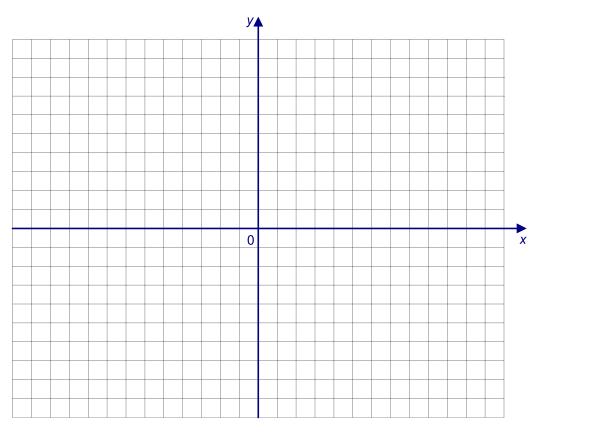
\includegraphics[ width=4.8663in, height=3.4956in,]{L4SZ2705}
	}
	\begin{enumerate}
		\item Show the points $A \left (3 ,5\right )$ and $B \left ( -2 , -5\right )$ on the graph. 
		
		\item Calculate the slope of the line through $A$ and $B$. i.e. the slope of $\bar{AB}\text{.}$ 
		
		\item What is the equation of the line $A B$? 
		
		\item What is the equation of the line parallel to the line $A B$ through the point $\left ( -2 ,3\right )\text{?}$ 
		
		\item Starting from the point $B$ on the graph frame draw a line with a slope of $\frac{4}{5}\text{.}$ 
	\end{enumerate}

  	
	\item 
	If $f (x) =x^{2}$ and $g (x) =x^{3}$ evaluate 
	
	
	\begin{enumerate}
		\item $f (2)$ 
		
		\item $f ( -2)$ 
		
		\item $g (3)$ 
		
		\item $g ( -3)\vspace{+5.000000cm}$ \end{enumerate}
	
	
	\item 
	Complete the table of values for the function $g (x) =x^{3} -x$ and sketch the graph\vspace{0.5cm} \\\relax
	\begin{tabular}[c]{cc}\hline
		$x$  & $g (x) =x^{3} -x$  \\
		\hline
		$ -1.5\rule[-8pt]{0pt}{24pt}$  & \ \ \ \ \ \ \ \ \ \ \ \ \ \ \ \ \ \ \  \\
		\hline
		$ -1\rule[-8pt]{0pt}{24pt}$  &  \\
		\hline
		$ -0.5\rule[-8pt]{0pt}{24pt}$  &  \\
		\hline
		$0\rule[-8pt]{0pt}{24pt}$  &  \\
		\hline
		$0.5\rule[-8pt]{0pt}{24pt}$  &  \\
		\hline
		$1\rule[-8pt]{0pt}{24pt}$  &  \\
		\hline
		$1.5\rule[-8pt]{0pt}{24pt}$  &  \\
		\hline
	\end{tabular} \\\relax
	\setlength\fboxrule{0in}\setlength\fboxsep{0.2in}\fcolorbox[HTML]{000000}{FFFFFF}{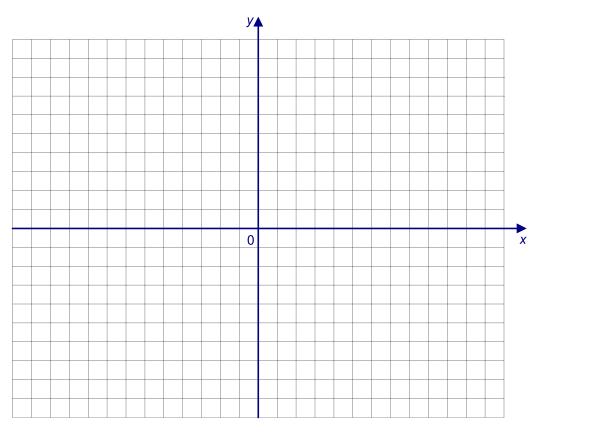
\includegraphics[ width=4.8663in, height=3.4956in,]{L4SZ2706}
	}
	 
	
	\item  Given $f (x) =\left (x +3)(x -1\right )\left (x +1\right )^{2}$ 
	

	\begin{enumerate}
		\item What is the degree of the polynomial? 
		
		\item Where does
		the graph cut the $x$-axis? (I.e. what are the zeros?) 
		
		\item Where does the graph cut the $y$-axis? 
		
		\item Sketch the graph \\\relax
		\setlength\fboxrule{0in}\setlength\fboxsep{0.2in}\fcolorbox[HTML]{000000}{FFFFFF}{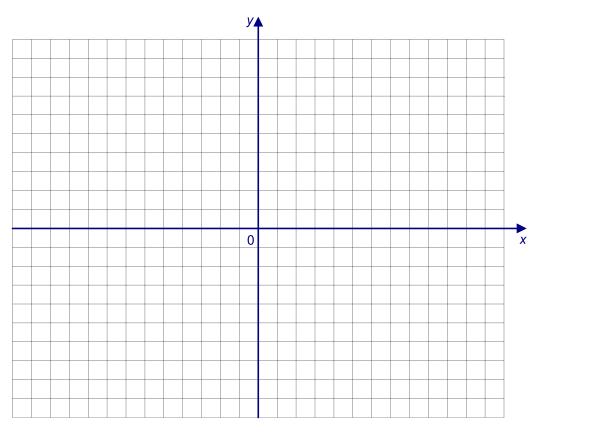
\includegraphics[ width=4.561in, height=3.2759in,]{L4SZ2707}
		}
	\end{enumerate}

	\item Fill in the
	table and draw the graph of $y =\genfrac{(}{)}{}{}{1}{2}^{x}\vspace{+0.500000cm}$ \\\relax
	\begin{tabular}[c]{|c|c|c|c|c|c|c|c|}\hline
		$x$  & -3  & -2  & -1
		& 0  & 1  & 2  & 3
		\\
		\hline
		$y =\genfrac{(}{)}{}{}{1}{2}^{x}$  & \ \ \ \ \ \rule[-8pt]{0pt}{24pt}
		& \ \ \ \ \ \rule[-8pt]{0pt}{24pt}
		& \ \ \ \ \ \rule[-8pt]{0pt}{24pt}
		& \ \ \ \ \ \rule[-8pt]{0pt}{24pt}
		& \ \ \ \ \ \rule[-8pt]{0pt}{24pt}
		& \ \ \ \ \ \rule[-8pt]{0pt}{24pt}
		& \ \ \ \ \ \rule[-8pt]{0pt}{24pt}
		\\
		\hline
	\end{tabular} \\\relax
	\setlength\fboxrule{0in}\setlength\fboxsep{0.2in}\fcolorbox[HTML]{000000}{FFFFFF}{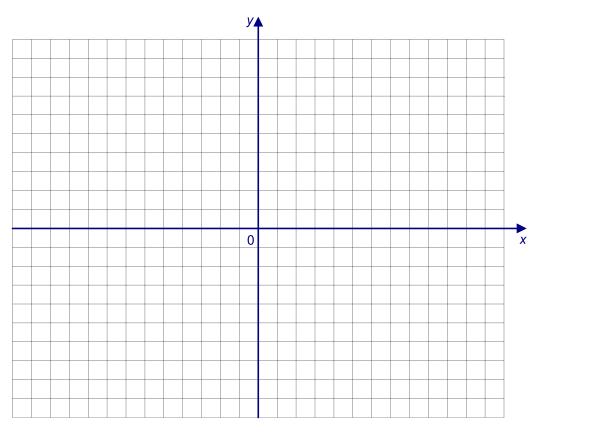
\includegraphics[ width=4.4771in, height=3.2162in,]{L4SZ2708}
	}
	
	
	
	\begin{enumerate}
		\item [(b)] Evaluate 
		
		
		\begin{enumerate}
			\item $3^{3.4}$ 
			
			\item $e^{ -0.6}$ \end{enumerate}
	\end{enumerate}
	
	
	\item 
	Write the equivalent logarithm statement. One is done for you. 
	
	
	\begin{enumerate}
		\item
		\begin{enumerate}
			\item $64 =2^{6} \Leftrightarrow \log _{2} 64 =6$ 
			
			\item $0.01 =10^{ -2} \Leftrightarrow $ \end{enumerate}
		
		
		\item [(b)]
		Write the equivalent statement using an exponent. 
		
		
		\begin{enumerate}
			\item $\log _{5} 625 =4 \Leftrightarrow $ 
			
			\item $\log _{a} k =t \Leftrightarrow $ \end{enumerate}
		
		
		\item [(c)]
		Calculate the value for 
		
		
		\begin{enumerate}
			\item $\log _{9} 9$ 
			
			\item $\log _{2} \genfrac{(}{)}{}{}{1}{8}$ 
			
			\item $\log  1000$ 
			
			\item $\ln  2.95$ 
			
			\item $\ln  e^{3.1}$ 
			
			\item $\log _{4} 0.25$ \end{enumerate}
	\end{enumerate}

	\item Write the following as the logarithm of a single number 
	
	
	\begin{enumerate}
		\item $\log _{4} 7 +\log _{4} 5$ 
		
		\item $\log _{5} 18 -\log _{5} 3$ 
		
		\item $2 \log _{3} 4$ 
		
		\item $\log _{4} 5 +\log _{4} 2 -\log _{4} 10 +3 \log _{4} 2$ \end{enumerate}	
\end{enumerate}

\section{Some Answers}
\begin{tabular}[c]{rrlr}1.  & (a)
	& $ -x -y$  &  \\
	& (b)
	& $ -15 x +6 y$  &  \\
	&  &  &  \\
	2.
	&  & $2\frac{1}{2}$  &  \\
	&  &  &  \\
	3.
	& (a)  & $1$  &  \\
	& (b)
	& $0.01$  &  \\
	&  &  &  \\
	4.
	& (a)  & $9 a^{4} b^{2}$  &  \\
	& (b)
	& $\frac{x^{6}}{27}$  &  \\
	&  &  &  \\
	5.
	&  & $1.28$  &  \\
	&  &  &  \\
	6.
	& (a)  & $x^{2} +3 x +2$  &  \\
	& (b)
	& $4 x^{2} -1$  &  \\
	&  &  &  \\
	7.
	& (a)  & $\left (x +7\right ) \left (x +4\right )$  &  \\
	& (b)
	& $\left (2 x +3\right ) \left (x -4\right )$  &  \\
	&  &  &  \\
	8.
	&  & $\frac{x +2}{x -1}$  &  \\
	&  &  &  \\
	9.
	& (a)  & $3.16$  &  \\
	& (b)
	& $ -1.87$ or $5.87$  &  \\
	&  &  &  \\
	10.
	& (a)  & $4$ or $ -2$  &  \\
	& (b)
	& $0.637$ or $ -3.137$  &  \\
	&  &  &  \\
	11.
	& (a)  & $t =\frac{v -u}{a}$  &  \\
	& (b)
	& $t =\frac{1}{\alpha } \left (\frac{l}{l_{0}} -1\right )$  &  \\
	&  &  &  \\
	12.
	&  & $79.4 \mathrm{m}^{3}$  &  \\
	&  &  &  \\
	13.
	&  & Parabola with vertex $\left (0 , -3\right )$  & 
\end{tabular}

\relax    
\setlength\fboxrule{0.01in}\setlength\fboxsep{0.2in}\fcolorbox[HTML]{000000}{FFFFFF}{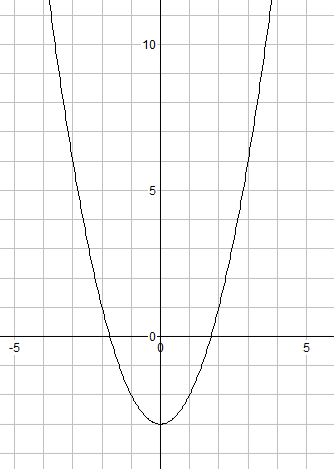
\includegraphics[ width=2.0496in, height=2.8669in,]{L4SZ2709}
}
\\ 
\\



\begin{tabular}[c]{rrlr}14.  &  & $3.61$  &  \\
	&  &  &  \\
	15.
	&  & x-intercepts $1.73$ and $ -1.73$  &  \\
	&  & y-intercept
	$ -3$  &  \\
	&  &  &  \\
	16.
	& (a)  & On the graph below  &  \\
	& (b)
	& $2$  &  \\
	& (c)
	& $y =2 x -1$  &  \\
	& (d)
	& $y =2 x +7$  & 
\end{tabular}

16. (e)
\setlength\fboxrule{0.01in}\setlength\fboxsep{0.2in}\fcolorbox[HTML]{000000}{FFFFFF}{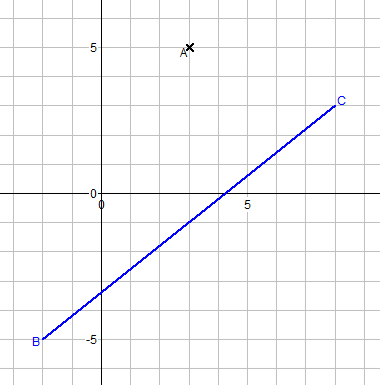
\includegraphics[ width=2.8297in, height=2.8669in,]{L4SZ270A}
}
\\ 
\\



\begin{tabular}[c]{rrrr}17.  & (a)
	& $4$  &  \\
	& (b)
	& $4$  &  \\
	& (c)
	& $27$  &  \\
	& (d)
	& $ -27$  & 
\end{tabular}

18.
\begin{tabular}[c]{|c|c|}\hline
	$x$  & $g (x) =x^{3} -x$  \\
	\hline
	$ -1.5$  & $ -1.875\;$  \\
	\hline
	$ -1$  & $0$  \\
	\hline
	$ -0.5$  & $0.375$  \\
	\hline
	$0$  & $0$  \\
	\hline
	$0.5$  & $ -0.375$  \\
	\hline
	$1$  & $0$  \\
	\hline
	$1.5$  & $1.875$  \\
	\hline
\end{tabular}\vspace{0.5cm} \\\relax
\setlength\fboxrule{0.01in}\setlength\fboxsep{0.2in}\fcolorbox[HTML]{000000}{FFFFFF}{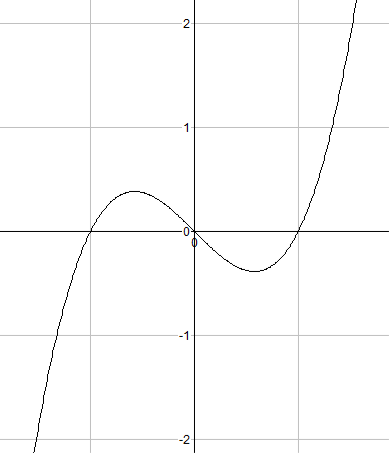
\includegraphics[ width=2.4656in, height=2.866in,]{L4SZ270B}
}


$
\begin{tabular}[c]{rrlr}19. 
& (a)
& $4$
& 
\\
& (b)
& $ -3$, $1$, $ -1$ (touches) 
& 
\\
& (c)
& $ -3$
& 
\end{tabular}\vspace{+0.500000cm}$ 

19.(d)    
\setlength\fboxrule{0.01in}\setlength\fboxsep{0.2in}\fcolorbox[HTML]{000000}{FFFFFF}{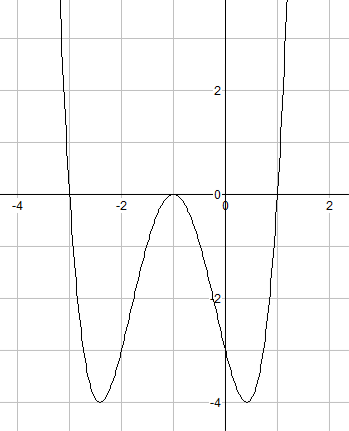
\includegraphics[ width=2.3263in, height=2.866in,]{L4SZ270C}
}


20. (a) $8 ,4 ,2 ,1 ,\frac{1}{2} ,\frac{1}{4} ,\frac{1}{8}\vspace{+0.500000cm}$ \\\relax    
\setlength\fboxrule{0.01in}\setlength\fboxsep{0.2in}\fcolorbox[HTML]{000000}{FFFFFF}{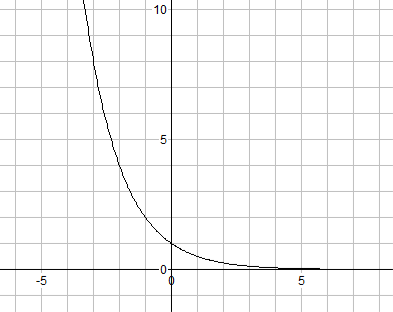
\includegraphics[ width=3.1782in, height=2.5278in,]{L4SZ270D}
}



\begin{tabular}[c]{rrrl}20.  & (b)
	& 1.  & $41.9$  \\
	&  & 2.
	& $0.5488$  \\
	&  &  &  \\
	21.
	& (a)  &  & $\log _{10} 0.01 = -2$  \\
	& (b)  & 1.
	& $625 =5^{4}$  \\
	&  & 2.
	& $k =a^{t}$  \\
	& (c)  & 1.
	& $1$  \\
	&  & 2.
	& $ -3$  \\
	&  & 3.
	& $3$  \\
	&  & 4.
	& $1.082$  \\
	&  & 5.
	& $3.1$  \\
	&  & 6.
	& $ -1$  \\
	&  &  &  \\
	22.
	& (a)  &  & $\log _{4} 35$  \\
	& (b)  &  & $\log _{5} 6$  \\
	& (c)  &  & $\log _{3} 16$  \\
	& (d)  &  & $\log _{4} 8$  \\
	&  &  &  \\

\end{tabular} 

\section{Factoring Exercises}
Some exercises look quite difficult on the surface but quickly look like a
familiar one once you get started. 

\subsubsection{Example}
Completely factor the following expression: $x^{4} +2 x^{3} -3 x^{2}$\\
Start by removing the common factor to all terms: $x^2$\\
\begin{eqnarray*}  &= x^{2} \left (x^{2} +2 x -3\right ) \\
	 &= x^{2} \left (x -1\right ) \left (x +3\right )\end{eqnarray*}


Solve the following equations both algebraically and graphically.

\begin{enumerate}
	\item   
	\columnsep =30pt
	\begin {multicols}{2}
	$x -4 =5 x +12$ 
	
	\item $\frac{1}{2} x -3 =6 +2 x$ 
	
	\item $\frac{2}{x} +\frac{1}{2 x} =7$ 
	
	\item $\frac{4}{x +2} -\frac{6}{2 x} =\frac{5}{2 x +4}$ 
	
	\item $x^{2} -32 =0$ 
	
	\item $x^{3} +16 =0$ 
	
	\item $16 x^{4} =625$ 
	
	\item $2 x^{5} -243 =0$ 
	
	\item $\left (x -5\right )^{4} -80 =0$ 
	
	\item $6 \left (x +2\right )^{5} =64$ 
	\end {multicols}

\end{enumerate}


Find all real solutions of these equations correct to two decimal places (d.p.). 


\begin{enumerate}
	\setcounter{enumi}{10}\item  
	\columnsep =30pt
	\begin {multicols}{2}
	$x^{3} -2 x^{2} -x -1 =0$ 
	
	\item $x^{4} -8 x^{2} +2 =0$ 
	
	\item $x \left (x -1\right ) \left (x +2\right ) =\frac{1}{6} x$ 
	
	\item $x^{4} =16 -x^{3}$ 
	\end {multicols}

\end{enumerate}


Solve these inequalities correct to two d.p. 
\begin{enumerate}
	\setcounter{enumi}{14}\item   
	\columnsep =30pt
	\begin {multicols}{2}
	$x^{2} -3 x -10 \leq 0$ 
	
	\item $0.5 x^{2} +0.875 x \leq 0.25$ 
	
	\item  $x^{3} +11 x \leq 6 x^{2} +6$ 
	
	\item $16 x^{3} +24 x^{2} > -9 x -1$ 
	
	\item  $x^{\frac{1}{3}} <x$ 
	
	\item  $\left (x +1\right )^{2} <\left (x -1\right )^{2}$ 
	\end {multicols}

\end{enumerate}

\chapter{Systems of Equations}

A system of equations means having more than one relationship representing the system of interest. We will study systems composed of 2 linear equations and 2 unknowns. Systems with more equations and more variables are possible and will be covered in future courses. Three approaches to solve systems of equations will be covered here:
\begin{itemize}
	\item substitution
	\item elimination
	\item graphing
\end{itemize}

You could be asked to solve a system of 2 equations with 2 unknowns where one equation is linear and the other is not. Also you could be asked to solve a system of two nonlinear
equations although these will be restricted to very straightforward examples. It helps if you can visualise
the shape of the 2 equations so that the meaning of the solution is clear in your mind. An example will come later in the course when we find the area between two curves by integration where the intersection of these two curves represents the solution to a system of two equations.

We know that linear equations in two variables are represented by straight lines. Straight
lines will always intersect unless they are parallel. The coordinates of the point of intersection of the straight
lines is called the solution. you could use a graphical method or one of the two algebraic methods (substitution
or elimination) to find the solution. Parallel lines will never meet so will have no solution. Sometimes
the two equations will be two different representations of the same line so we say that in this case the system has an infinite number of solutions. 

\section{Solution by Substitution}
\subsubsection{Example 1}
Consider the system of equations
\begin{align}x^{2} +y^{2} &  = 25 \tag{1} \\
3 y +x &  = 15 \tag{2}\end{align}

We rearrange equation 2 and substitute into equation 1
\begin{align*}x &  =  15 -3 y \\
	&  =  3 \left (5 -y\right ) \\
	\text{so }\quad x^{2} &  =  9 \left (25 -10 y +y^{2}\right ) \\
	&  =  9 y^{2} -90 y +225\end{align*}

Equation 1 becomes
\begin{align*}9 y^{2} -90 y +225 +y^{2} &  =  25 \\
	10 y^{2} -90 y +200 &  =  0 \\
	y^{2} -9 y +20 &  = 0 \\
	\left (y -5\right ) \left (y -4\right ) &  =  0 \\
	\text{Either }\quad y -5 &  =  0\quad\text{ so }\quad y =5 \\
	\text{or }\quad y -4 &  =  0\quad\text{ so }\quad y =4\end{align*}

Back-substitute into equation 2 

When $y =5$, $3 y +x =15 \leadsto 15 +x =15 \Longleftrightarrow x =0$. This means $\left (0 ,5\right )$ is a solution. 

When $y =4$, $3 y +x =15 \leadsto 12 +x =15 \Longleftrightarrow x =3$. This means $\left (3 ,4\right )$ is a solution. 

\subsubsection{Example 2}
Now consider the system of equations
\begin{align}x^{2} +y^{2} &  =  25 \tag{3} \\
4 y +3 x &  =  25 \tag{4}\end{align}

Proceeding in the same way
\begin{align*}3 x &  =  25 -4 y \\
	\text{So\ \ \ }9 x^{2} &  =  \left (25 -4 y\right )^{2} \\
	&  =  625 -200 y +16 y^{2} \\
	&  =  16 y^{2} -200 y +625\end{align*}

From equation 3\qquad (Multiply equation 3 by 9)
\begin{align*}9 x^{2} +9 y^{2} &  =  225 \\
	\text{So}\quad 16 y^{2} -200 y +625 +9 y^{2} &  = 225\text{\ }{\tiny 9}{\tiny x}^{{\small 2}}\text{} \\
	\text{or}\quad 25 y^{2} -200 y +625 -225 &  =  0 \\
	25 y^{2} -200 y +400 &  =  0\text{\ \ } \\
	\text{or} \quad y^{2} -8 y +16 &  = 0 \\
	\left (y -4\right ) \left (y -4\right ) &  = 0 \\
	\text{So}\quad y &  =  4\end{align*}

Back substitute into equation 4 

When $y =4$, $4 y +3 x =25 \leadsto 16 +3 x =25 \Longleftrightarrow x =3$. This means $\left (3 ,4\right )$ is a solution. The
line cuts the circle in only one point. This means the line touches the circle. The
line is a tangent to the circle. You may verify by graphing the functions.

\subsection{Exercise}
\begin{enumerate}
	\item How can we invent a line parallel to $4 y +3 x =25$ that cuts the circle (in two points)? 
	
	\item How can we invent a line parallel
	to $4 y +3 x =25$ that misses the circle (cuts the circle in no points)? \end{enumerate}


Solution:
\ There are an infinite number of possibilities one such line that will cut the circle in two points is $4 y +3 x =24$, and a line that will miss the circle is $4 y +3 x =26$. 

\section{Solution by Elimination}
Refer to lecture notes.
\section{Solution by Graphing}
Refer to lecture notes.
\section{Infinite Solutions}
\emph{Example of a System with an Infinite Number of Solutions}\\
If you start with a linear equation such as $y -2 x =3$ and multiply each term by a constant you will get an equivalent equation. If you multiply the equation by another number you
will get a further equivalent equation.
\begin{equation*}y -2 x =3
\end{equation*}

Multiply by $2$
\begin{equation*}2 y -4 x =6
\end{equation*}

Multiply by $ -3$
\begin{align*} -3 y +6 x &  = &  -9 \\
\text{or}6 x -3 y +9 &  = & 0\end{align*}

We know these are both just different ways of writing the original equation $y -2 x =3$ or $y =2 x +3$. To say the system has an infinite number of solutions we are really saying every point
on $y =2 x +3$ is a solution. 


%
%We have a further way to represent these equations which we will introduce here. It
%is called the \emph{parametric} form of a straight line. In mathematics we like to have as
%few variables as we can and you have already seen many instances where we have started off with two variables and by using a relationship given within the
%problem we have reduced the number of variables to one. By introducing a \emph{parameter}
%we can reduce from two variables ($x$ and $y$) to one. Here is a simple procedure to introduce a parameter. We
%usually use the letter $t$ to represent a parameter ( but this is not always the case). Let $x =t$ and $y =2 t +3$ then we can immediately say that the point $\left (t ,2 t +3\right )$ lies on the line $y =2 x +3$ $ \forall t \in \mathbb{R}$ $\left [\text{The literal translation of} \forall \text{is "for all values of", so} \forall t \in \mathbb{R}\text{means "for real values of}t\text{"}\right ]$ What this means is
%that you can take any value of $t$ you like and substitute it into $\left (t ,2 t +3\right )$ and you will get a point on the line $y =2 x +3$. 



\section{Guidelines for Solving Systems of Equations}
These guideline provide a useful way to tackle any problems where equations are involved. 

\begin{enumerate}
	\item Identify the variables. We often call them $x$ and $y$, but you may chose any name or letter you want. 
	
	\item Express all unknown quantities
	in terms of the variables. 
	
	\item Set up a system of equations using the facts provided by the problem.
	
	
	\item Solve the system of equations and use the solution to check it satisfies the conditions of the
	problem. Write a sentence describing the answer to the original problem.  
\end{enumerate}


\subsubsection{Example}
This is about a boat travelling with the current and against the current and depends
on you knowing that velocities are vectors so can be added and subtracted. 


\begin{description}
	\item [Step 1] Let the speed of the boat be $x$ \mbox{mi}$/$\mbox{h} and the speed of the current be $y$ \mbox{mi}$/$\mbox{h}. 
	
	\item [Step
	2]
	\begin{align*}\text{Upstream speed} &  =  x -y \\
	\text{Downstream speed} &  =  x +y\end{align*}
	
	\item [Step 3]
	\begin{align}\text{Speed} &  =  \frac{\text{Total distance}}{\text{Total time}} \nonumber  \\
	\text{so Total distance} &  =  \text{Speed} \times \text{Total time} \nonumber  \\
	20 &  =  \left (x +y\right ) \times 1 \nonumber  \\
	20 &=x +y \tag{1} \\
	\text{Also}\quad 20 &  =  \left (x -y\right ) \times \frac{5}{2} \nonumber  \\
	8 &=x -y \tag{2}\end{align}
	
	\item [Step 4] \end{description}

Eq 1 + Eq 2
\begin{align*}28 &  =  2 x \\
x &  =  14 \\
y &  =  6\end{align*}

\textbf{Check:} \\\relax The boat travels
at 14 $\mbox{mi}$/$\mbox{h}$ and the current travels at 6 $\mbox{mi}$/$\mbox{h}$ so the effective speed of the
boat is 20 $\mbox{mi}$/$\mbox{h}$. At 20 $\mbox{mi}$/$\mbox{h}$ the 20 $\mbox{mi}$ trip took $1$ $\mbox{h}$. Upstream the speed is 8 $\mbox{mi}$/$\mbox{h}$. \
\begin{align*}\text{Total time} &  =  \frac{\text{Total distance}}{\text{Speed}} \\
&  =  \frac{20}{8} =\frac{5}{2} \text{ h}\end{align*}

Therefore the speed of the boat is 14 $\mbox{mi}$/$\mbox{h}$ and the speed of the current is 6 $\mbox{mi}$/$\mbox{h}$. 


\section{Exercises}
Solve the following linear systems of two equations with two unknowns using an appropriate method.
\begin{description}
\columnsep =30pt
\begin {multicols}{2}
	\item [a.]   	
	$\left \{
	\begin{tabular}[c]{rrr}$x +y$
	& $ =$
	& $4$
	\\
	$2 x -y$
	& $ =$
	& $2$
	\end{tabular}\right .$ \\
	
	\item [b.]
	$\left \{
	\begin{tabular}[c]{rrr}$2 x +y$
	& $ =$
	& $11$
	\\
	$x -2 y$
	& $ =$
	& $4$
	\end{tabular}\right .$ \\
	

	\item [c.]   	
	$\left \{
	\begin{tabular}[c]{rrr}$2 x -3 y$
	& $ =$
	& $12$
	\\
	$ -x +\frac{3}{2} y$
	& $ =$
	& $4$
	\end{tabular}\right .$ \\
	
	\item [d.]
	$\left \{
	\begin{tabular}[c]{rrr}$2 x +6 y$
	& $ =$
	& $0$
	\\
	$ -3 x -9 y$
	& $ =$
	& $18$
	\end{tabular}\right .$ \\
	
	\item [e.]   
	$\left \{
	\begin{tabular}[c]{rrr}$ -x +\frac{1}{2} y$
	& $ =$
	& $ -5$
	\\
	$2 x -y$
	& $ =$
	& $10$
	\end{tabular}\right .$ \\
	
	\item [f.]
	$\left \{
	\begin{tabular}[c]{rrr}$12 x +15 y$
	& $ =$
	& $ -18$
	\\
	$2 x + 5 y$
	& $ =$
	& $ -3$
	\end{tabular}\right .$ \\
	\end {multicols}
	
\end{description}

Use the substitution method to find all solutions of the system of equations. *Note that some are non-linear equations.

\begin{description}

	\columnsep =30pt
	\begin {multicols}{2}
	\item [1.]   
		$\left \{
	\begin{tabular}[c]{rrr}$x -y$
	& $ =$
	& $2$
	\\
	$2 x +3 y$
	& $ =$
	& $9$
	\end{tabular}\right .$ 
	
	\item [3.]
	$\left \{
	\begin{tabular}[c]{lll}$y$
	& $ =$
	& $x^{2}$
	\\
	$y$
	& $ =$
	& $x +12$
	\end{tabular}\right .$ 
	\end {multicols}
	
	
	\item [5.]   
	\columnsep =30pt
	\begin {multicols}{2}
	%EndExpansion
	$\left \{
	\begin{tabular}[c]{rrr}$x^{2} +y^{2}$
	& $ =$
	& $8$
	\\
	$x +y$
	& $ =$
	& $0$
	\end{tabular}\right .$ 
	
	\item [7.]
	$\left \{
	\begin{tabular}[c]{rrr}$x +y^{2}$
	& $ =$
	& $0$
	\\
	$2 x +5 y^{2}$
	& $ =$
	& $75$
	\end{tabular}\right .$ 
	\end {multicols}

\end{description}

Use the elimination method to find
all solutions of the system of equations 


\begin{description}
	\item [9.]   
	%TCIMACRO{\TeXButton{Start Two Columns}{\columnsep =30pt
	% \begin {multicols}{2}}}%
	%BeginExpansion
	\columnsep =30pt
	\begin {multicols}{2}
	%EndExpansion
	$\left \{
	\begin{tabular}[c]{rrr}$x +2 y$
	& $ =$
	& $5$
	\\
	$2 x +3 y$
	& $ =$
	& $8$
	\end{tabular}\right .$ 
	
	\item [11.]
	$\left \{
	\begin{tabular}[c]{rrr}$x^{2} -2 y$
	& $ =$
	& $1$
	\\
	$x^{2} +5 y$
	& $ =$
	& $29$
	\end{tabular}\right .$ 
	%TCIMACRO{\TeXButton{End Two Columns}{\end {multicols}}}%
	%BeginExpansion
	\end {multicols}
	%EndExpansion
	
	
	\item [13.] $\left \{
	\begin{tabular}[c]{rrr}$3 x^{2} -y^{2}$
	& $ =$
	& $11$
	\\
	$x^{2} +4 y^{2}$
	& $ =$
	& $8$
	\end{tabular}\right .$ \end{description}

Find all solutions of the system of equations 


\begin{description}
	\item [17.]   
	%TCIMACRO{\TeXButton{Start Two Columns}{\columnsep =30pt
	% \begin {multicols}{2}}}%
	%BeginExpansion
	\columnsep =30pt
	\begin {multicols}{2}
	%EndExpansion
	$\left \{
	\begin{tabular}[c]{rrr}$y +x^{2}$
	& $ =$
	& $4 x$
	\\
	$y +4 x$
	& $ =$
	& $16$
	\end{tabular}\right .$ 
	
	\item [18.]
	$\left \{
	\begin{tabular}[c]{rrr}$x -y^{2}$
	& $ =$
	& $0$
	\\
	$y -x^{2}$
	& $ =$
	& $0$
	\end{tabular}\right .$ 
	%TCIMACRO{\TeXButton{End Two Columns}{\end {multicols}}}%
	%BeginExpansion
	\end {multicols}
	%EndExpansion
	
	
	\item [21.]   
	%TCIMACRO{\TeXButton{Start Two Columns}{\columnsep =30pt
	% \begin {multicols}{2}}}%
	%BeginExpansion
	\columnsep =30pt
	\begin {multicols}{2}
	%EndExpansion
	$\left \{
	\begin{tabular}[c]{rrr}$x -y$
	& $ =$
	& $4$
	\\
	$x y$
	& $ =$
	& $12$
	\end{tabular}\right .$ 
	
	\item [25.]
	$\left \{
	\begin{tabular}[c]{rrr}$x^{2} +y^{2}$
	& $ =$
	& $9$
	\\
	$x^{2} -y^{2}$
	& $ =$
	& $1$
	\end{tabular}\right .$ 
	%TCIMACRO{\TeXButton{End Two Columns}{\end {multicols}}}%
	%BeginExpansion
	\end {multicols}
	%EndExpansion
\end{description}

Use a graphical method to find all solutions of the system of equations correct
to 2 decimal places 


\begin{description}
	\item [31.]   
	%TCIMACRO{\TeXButton{Start Two Columns}{\columnsep =30pt
	% \begin {multicols}{2}}}%
	%BeginExpansion
	\columnsep =30pt
	\begin {multicols}{2}
	%EndExpansion
	$\left \{
	\begin{tabular}[c]{rrr}$y$
	& $ =$
	& $2 x +6$
	\\
	$y$
	& $ =$
	& $ -x +5$
	\end{tabular}\right .$ 
	
	\item [35.]
	$\left \{
	\begin{tabular}[c]{rrr}$x^{2} +y^{2}$
	& $ =$
	& $25$
	\\
	$x +3 y$
	& $ =$
	& $2$
	\end{tabular}\right .$ 
	%TCIMACRO{\TeXButton{End Two Columns}{\end {multicols}}}%
	%BeginExpansion
	\end {multicols}
	%EndExpansion
	
	
	\item [37.] $\left \{
	\begin{tabular}[c]{lrr}$\frac{x^{2}}{9} +\frac{y^{2}}{18} =1$
	& 
	& 
	\\
	$y = -x^{2} +6 x -2$
	& 
	& 
	\end{tabular}\right .$ \end{description}

Word problems 


\begin{description}
	\item [41.] A rectangle has an area of $180 cm^{2}$ and a perimeter of $54 \mbox{cm}$. What are its dimensions? 
	
	\item [42.]
	A right-angled triangle has an area of $84 cm^{2}$ and a hypotenuse $25 \mbox{cm}$ long. What are the lengths of the other two sides?
	
	
	\item [44.] A circular piece of sheet metal has a diameter
	of $20 \mbox{cm}$. the edges are to be cut off to form a rectangle
	of area $160 cm^{2}$. What are the dimensions of the rectangle? 
	
	\item \qquad \qquad \qquad \qquad \qquad \qquad
	\setlength\fboxrule{0in}\setlength\fboxsep{0.2in}\fcolorbox[HTML]{000000}{FFFFFF}{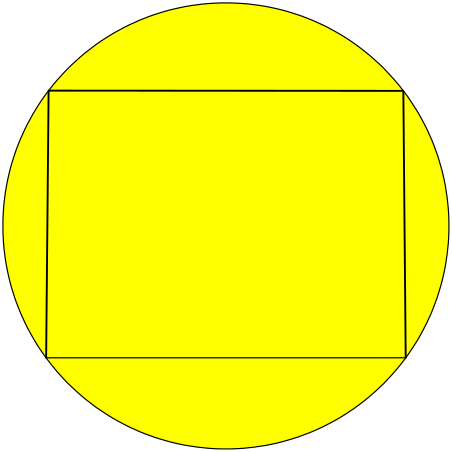
\includegraphics[ width=2.6385in, height=2.6385in,]{L4SZ270E}
	}
	
	
	\item [46.] A rectangular piece of sheet metal with and
	area of $1200 cm^{2}$ is to be bent into a cylindrical length of pipe having a volume of $600 cm^{3}$. What are the dimensions of the sheet of metal? \end{description}

\begin{description}
	\item [47.] The admission fee at an amusement park is $ \$1.50$ for children and $ \$4.00$ for adults. On a certain day, $2200$ people entered the park and the admission fees collected totalled $ \$5050$. How many children and how many adults were admitted? 
	
	\item [48.]
	A man flies a small aeroplane from Fargo to Bismarck, North Dakota - a distance of $180 \mbox{mi}$. Because he is flying into a headwind, the trip
	takes him $2$ hours. On the way back, the wind is still blowing at the same speed, so the return
	trip takes only $1$ hour and $12$ minutes. What is his speed in still air and how fast is the wind blowing? 
	
	\item [49.]
	A woman keeps fit by bicycling and running every day. One Monday she spends $\frac{1}{2} \mbox{h}$ at each activity and covers a total of $12\frac{1}{2} \mbox{mi}$. On Tuesday she runs for $12 \mbox{min}$ and cycles for $45 \mbox{min}$, covering a total of $16 \mbox{mi}$. Assuming her running and cycling speeds don't
	change from day to day, find these speeds. 
	
	\item [50.] A customer
	in a coffee shop purchases a blend of two coffees: Kenyan, costing $ \$3.50$ a pound, and Sri Lankan, costing $ \$5.60$ a pound. He buys $3 \mbox{lb}$ of the blend, which costs him $ \$11.55$. How many pounds of each kind went into the mixture?
\end{description}


\section{Some Answers}

\columnsep =30pt
\begin {multicols}{2}

\textbf{Linear Only:}

a. $\left (2 ,2\right )$ 

b. $\left (5.2 ,0.6\right )$

c. no solutions

d. no solutions

e. infinite solutions

f. $\left (-1.5 ,0\right )$\\
\break
\textbf{Mixed:}

1. $\left (3 ,1\right )$ 

3. $\left (4 ,16\right )$ 

5. $\left (2 , -2\right ) ,\left ( -2 ,2\right )$ 

7. $\left ( -25 ,5\right ) ,\left ( -25 , -5\right )$ 

9. $\left (1 ,2\right )$ 

11. $\left ( -3 ,4\right ) ,\left (3 ,4\right )$ 

13. $\left ( -2 , -1\right ) ,\left ( -2 ,1\right ) ,\left (2 , -1\right ) ,\left (2 ,1\right )$ 

17. $\left (4 ,0\right )$ 

18. $\left (0 ,0\right ) ,\left (1 ,1\right )$ 

21. $\left (6 ,2\right ) ,\left ( -2 , -6\right )$ 

25. $\left (\sqrt{5} ,2\right )\left (\sqrt{5} , -2\right )$ 

31. $\left ( -0.33 ,5.33\right )$ 

35. $\left ( -4.51 ,2.17\right ) ,\left (4.91 , -0.97\right )$ 

37. $\left (1.23 ,3.87\right ) ,\left ( -0.35 , -4.21\right )$ \\
\break
\textbf{Word Problems}\\

41. $12 \mbox{cm}$ by $15 \mbox{cm}$ 

42. $7 \mbox{ft}$ and $24 \mbox{ft}$ 

44. $4 \sqrt{5} \mbox{in}$ by $8 \sqrt{5} \mbox{in}$ 

46. The dimensions of the sheet are $2 \pi $ by $\frac{600}{\pi }$  

47. The number of children admitted was 1500 and the number
of adults was 700. 

48. Plane's speed $120 mi/\mbox{h}$, wind speed $30 mi/\mbox{h}$ 

49. Run $5 mi/\mbox{h}$, cycle $20 mi/\mbox{h}$ 

50. $2.5$ pounds of Kenyan coffee and $0.5$ pounds of Sri Lankan coffee should be mixed. 



\end {multicols}

\columnsep =30pt
\begin {multicols}{2}

\end {multicols}


\chapter{Trigonometry}

In the first half of this chapter the three trigonometric functions (sine, cosine and tangent) will be viewed as functions of angles. The second half of the chapter will approach trigonometry as functions of real numbers.

\section{The Measurement of Angles}
It should come as no surprise that the convention for measuring angles should be the same as for measuring
the distance around the perimeter of the unit circle.. An angle is measured in degrees and is the amount of
rotation between two rays about a vertex. If the vertex is placed at the point $\left (0 ,0\right )$ and one ray is placed along the positive $x$-axis then we let the second ray go through the point $P (x ,y)$ on the unit circle so that the relationship between the angle and $t$ (see chapter $2$) can be established. The convention is that the positive direction for measuring
angles is anticlockwise and the negative direction for measuring angles is clockwise. You will be aware that
one complete cycle measures 360$\mbox{{\ensuremath{{}^\circ}}}$. One degree therefore is $\frac{1}{360}$\ of one complete cycle. In this subject the
word revolution is often used instead of cycle. Other terms with which you might be familiar are "a quarter
turn" for $90 \mbox{{\ensuremath{{}^\circ}}}$ and "a half turn" for $180 \mbox{{\ensuremath{{}^\circ}}}$. 

If you draw a unit circle (centre $\left (0 ,0\right )$ radius $1$) then you can draw the ray through any terminal point and show the relationship between $t$ and the angle at the vertex $\left (0 ,0\right )$. 

Definition: If the unit circle is drawn and the distance $t$ is measured around the perimeter from $\left (1 ,0\right )$ to the point $P (x ,y)$ then we say the angle is measured as $t$ \emph{radians}. 

The abbreviation for radians is $\mbox{rad}$. This abbreviation will be used in the examples.
Some books uses the term "angles in standard position" to describe this situation. We
will not define this term unless it is unavoidable and will stick to 'rad'.

Using the language of geometry, the unit circle is cut by two rays one through the points $\left (0 ,0\right )$ and $\left (1 ,0\right )$ and the other through the points $\left (0 ,0\right )$ and $P \left (x ,y\right )$.  
\columnsep =30pt
\begin {multicols}{2}
   
\setlength\fboxrule{0in}\setlength\fboxsep{0.2in}\fcolorbox[HTML]{000000}{FFFFFF}{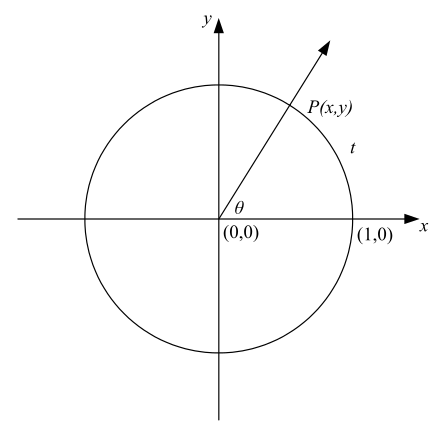
\includegraphics[ width=2.469in, height=2.4275in,]{L4SZ281A}
}

$t$ is referred to as "the length of the arc". The
angle $\theta $ between the two rays is referred to as "the angle \emph{subtended} at the point $\left (0 ,0\right )$". 

We will often leave out the word "subtended"
however this is because it is implied and we really should have used it. 


%TCIMACRO{\TeXButton{End Two Columns}{\end {multicols}}}%
%BeginExpansion
\end {multicols}
%EndExpansion


We can say therefore that the angle measured in radians is related to the same angle measured in degrees. the
relationship between these two measures must be understood and must be able to be derived. 

\subsection{Relationship between Degrees and Radians}
One complete revolution is 360$\mbox{{\ensuremath{{}^\circ}}}$ if the angle is measured in degrees and $2 \pi $ if the angle is measured in radians. So
\begin{align*}2 \pi \text{}\mbox{rad} &  =  360 \mbox{{\ensuremath{{}^\circ}}} \\
\text{or\  \ }\pi \text{}\mbox{rad} &  =  180 \mbox{{\ensuremath{{}^\circ}}}\end{align*}

You should derive this formula whenever you are asked to convert degrees to radians or radians
to degrees 

\subsubsection{Example}
(a) Convert 36$\mbox{{\ensuremath{{}^\circ}}}$ to radians 

(b) Convert $\frac{\pi }{3}$ $\mbox{rad}$ to degrees 

(c) Convert $1$ $\mbox{rad}$ to degrees 

(a)
\begin{align*}180 \mbox{{\ensuremath{{}^\circ}}} &  =  \pi \text{}\mbox{rad} \\
1 \mbox{{\ensuremath{{}^\circ}}} &  =  \frac{\pi }{180}\text{}\mbox{rad} \\
36 \mbox{{\ensuremath{{}^\circ}}} &  =  \frac{\pi }{180} \times 36 =\frac{\pi }{5}\text{}\mbox{rad}\end{align*}

(b)
\begin{align*}\pi  \mbox{rad} &  =  180 \mbox{{\ensuremath{{}^\circ}}} \\
\frac{\pi }{3} \mbox{rad} &  = \frac{180 \mbox{{\ensuremath{{}^\circ}}}}{3} =60 \mbox{{\ensuremath{{}^\circ}}}\end{align*}

(c)
\begin{align*}\pi  \mbox{rad} &  =  180 \mbox{{\ensuremath{{}^\circ}}} \\
1 \mbox{rad} &  =  \frac{180 \mbox{{\ensuremath{{}^\circ}}}}{\pi } \\
 &  \approx   57.29577951 \mbox{{\ensuremath{{}^\circ}}} \\
 &  \approx   57.3 \mbox{{\ensuremath{{}^\circ}}}\end{align*}

Note the similarity between the answers to (b) and (c). This
is because $\frac{\pi }{3} =1.047197551$ so you would expect the values in degrees to be similar. 



With this terminology we leave out the word measured when we talk about measuring angles. We
say "the angle is $60 \mbox{{\ensuremath{{}^\circ}}}$" when we mean it has been measured as $60 \mbox{{\ensuremath{{}^\circ}}}$ or "the angle is $\frac{\pi }{3}$" to mean it has been measured as $\frac{\pi }{3}$ $\mbox{rad}$. Notice we always put in the degree symbol and
often omit the units when the angle is measured in radians. Should units be omitted assume the angle is measured
in radians. We often use the Greek symbol $\theta $\ for the angle subtended at the centre of the unit circle so $\theta  =60 \mbox{{\ensuremath{{}^\circ}}}$ or $\theta  =\frac{\pi }{3}$ are further examples of terminology that is commonly used.

\subsection{Length of a Circular Arc}
Let $\theta $ be the angle subtended at the centre for the ends of an arc of any circle then the fraction of the circumference of the
circle is $\frac{\theta }{2 \pi }$ if $\theta $ is measured in radians and $\frac{\theta }{360 \mbox{{\ensuremath{{}^\circ}}}}$ if $\theta $ is measured in degrees. 

The length of the circumference of any circle whose radius is $r$ is $2 \pi  r$. 

If $\theta $ is measured in radians
\begin{equation*}\text{Length of arc} =\frac{\theta }{2 \pi } \times 2 \pi  r =\theta  r\text{ or }r \theta 
\end{equation*}

If $\theta $ is measured in degrees
\begin{equation*}\text{Length of arc} =\frac{\theta }{360 \mbox{{\ensuremath{{}^\circ}}}} \times 2 \pi  r
\end{equation*}

The simplicity of the first formula shows why working with radians is preferred. 

\subsubsection{Example}
Find the length of an arc that subtends an angle of 45$\mbox{{\ensuremath{{}^\circ}}}$ at the centre of a circle whose radius is 9 $\mbox{cm}\text{.}$ 

Method 1:
\begin{align*}\text{Length of arc} &  =  \frac{\theta }{360 \mbox{{\ensuremath{{}^\circ}}}} \times 2 \pi  r \\
 &  =  \frac{45}{360} \times 2 \pi  \times 9 \\
 &  =  2.25 \pi \text{}\mbox{cm} \\
 &  \approx   7.07\text{}\mbox{cm}\end{align*}

If an exact answer is required you should leave the answer as $2.25 \pi $ $\mbox{cm}$. (Or $\frac{9 \pi }{4}$ $\mbox{cm}\text{.}$) 

Method 2: Change degrees to radians first
\begin{align*}180 \mbox{{\ensuremath{{}^\circ}}} &  =  \pi \text{}\mbox{rad} \\
1 \mbox{{\ensuremath{{}^\circ}}} &  =  \frac{\pi }{180} \\
45 \mbox{{\ensuremath{{}^\circ}}} &  =  \frac{\pi }{180} \times 45 \\
 &  =  \frac{\pi }{4}\end{align*}


\begin{align*}\text{Length of arc} &  =  r \theta  \\
 &  =  9 \times \frac{\pi }{4} =\frac{9 \pi }{4}\text{}\mbox{cm}\end{align*}


\subsection{Area of Circular Sector}
It is assumed you know how to describe and visualise a sector of a circle and that you know that the area of a circle whose radius is $r$ is $\pi  r^{2}$. Continuing the logic above 

If $\theta $ is measured in radians
\begin{equation*}\text{Area of sector} =\frac{\theta }{2 \pi } \times \pi  r^{2} =\frac{1}{2} r^{2} \theta 
\end{equation*}

If $\theta $ is measured in degrees
\begin{equation*}\text{Area of sector} =\frac{\theta }{360 \mbox{{\ensuremath{{}^\circ}}}} \times \pi  r^{2}
\end{equation*}

\subsubsection{Example}
Find the area of a sector with a central angle of 45$\mbox{{\ensuremath{{}^\circ}}}$ for a circle whose radius is 4 $\mbox{cm}$. 

Method 1
\begin{align*}\text{Area of sector} &  =  \frac{45 \mbox{{\ensuremath{{}^\circ}}}}{360 \mbox{{\ensuremath{{}^\circ}}}} \times \pi  \times 4^{2} \\
 &  =  2 \pi \text{}cm^{2} \\
 &  \approx   6.28\text{ cm}^{2}\end{align*}

Method 2 As above
\begin{align*}180 \mbox{{\ensuremath{{}^\circ}}} &  =  \pi \text{}\mbox{rad} \\
1 \mbox{{\ensuremath{{}^\circ}}} &  =  \frac{\pi }{180} \\
45 \mbox{{\ensuremath{{}^\circ}}} &  =  \frac{\pi }{180} \times 45 \\
 &  =  \frac{\pi }{4}\end{align*}
\begin{align*}\text{Area of sector} &  =  \frac{1}{2} r^{2} \theta  \\
 &  =  \frac{1}{2} \times 4^{2} \times \frac{\pi }{4} \\
 &  =  2 \pi \text{ cm}^{2}\end{align*}



\subsection{Exercises}

Find the radian measure of the angle with the given degree measurements. 


\begin{description}
\item [1.]   
%TCIMACRO{\TeXButton{Start Two Columns}{\columnsep =30pt
% \begin {multicols}{2}}}%
%BeginExpansion
\columnsep =30pt
\begin {multicols}{2}
%EndExpansion
 $36 \mbox{{\ensuremath{{}^\circ}}}$ 

\item [3.]
$ -480 \mbox{{\ensuremath{{}^\circ}}}$ 
%TCIMACRO{\TeXButton{End Two Columns}{\end {multicols}}}%
%BeginExpansion
\end {multicols}
%EndExpansion
 

\item [5.]
%TCIMACRO{\TeXButton{Start Two Columns}{\columnsep =30pt
% \begin {multicols}{2}}}%
%BeginExpansion
\columnsep =30pt
\begin {multicols}{2}
%EndExpansion
 $60 \mbox{{\ensuremath{{}^\circ}}}$ 

\item [7.]
$ -135 \mbox{{\ensuremath{{}^\circ}}}$ 
%TCIMACRO{\TeXButton{End Two Columns}{\end {multicols}}}%
%BeginExpansion
\end {multicols}
%EndExpansion
 \end{description}

Find the degree measure of the angle with the given radian measure. 


\begin{description}
\item [9.]   
%TCIMACRO{\TeXButton{Start Two Columns}{\columnsep =30pt
% \begin {multicols}{2}}}%
%BeginExpansion
\columnsep =30pt
\begin {multicols}{2}
%EndExpansion
 $\frac{3 \pi }{4}$ 

\item [11.] $\frac{5 \pi }{6}$ 
%TCIMACRO{\TeXButton{End Two Columns}{\end {multicols}}}%
%BeginExpansion
\end {multicols}
%EndExpansion
 

\item [13.]
%TCIMACRO{\TeXButton{Start Two Columns}{\columnsep =30pt
% \begin {multicols}{2}}}%
%BeginExpansion
\columnsep =30pt
\begin {multicols}{2}
%EndExpansion
 $ -1.5$ 

\item [15.] $ -\frac{\pi }{12}$ 
%TCIMACRO{\TeXButton{End Two Columns}{\end {multicols}}}%
%BeginExpansion
\end {multicols}
%EndExpansion
 

\item [41.]
%TCIMACRO{\TeXButton{Start Two Columns}{\columnsep =30pt
% \begin {multicols}{2}}}%
%BeginExpansion
\columnsep =30pt
\begin {multicols}{2}
%EndExpansion
 Find the length of the arc $s$ in the figure. \\\relax The radius is $5$. 

\item    
\setlength\fboxrule{0in}\setlength\fboxsep{0.2in}\fcolorbox[HTML]{000000}{FFFFFF}{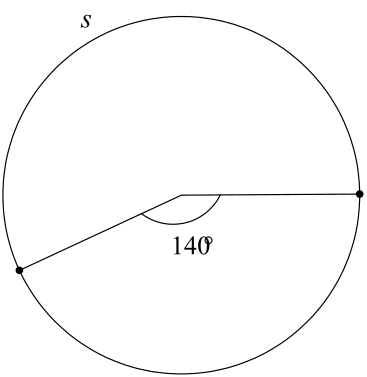
\includegraphics[ width=1.8057in, height=1.8507in,]{L4SZ281B}
}


\item [43.] Find the radius $r$ of the circle in the figure. 

\item    
\setlength\fboxrule{0in}\setlength\fboxsep{0.2in}\fcolorbox[HTML]{000000}{FFFFFF}{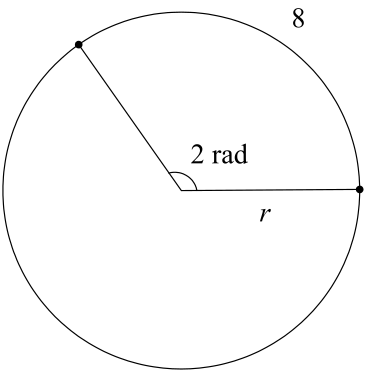
\includegraphics[ width=1.8196in, height=1.8438in,]{L4SZ281C}
}
%TCIMACRO{\TeXButton{End Two Columns}{\end {multicols}}}%
%BeginExpansion
\end {multicols}
%EndExpansion
 

\item [45.]
Find the length of an arc that subtends a central angle of $2 \mbox{rad}$ in a circle of radius 2mi. 

\item [47.]
An arc of length $100 \mbox{m}$ subtends a central angle in
a circle of radius $50 \mbox{m}$. Find the measure of $\theta $\ in degrees and in radians. 

\item [49.]
Find the radius of the circle if an arc of length $6 \mbox{m}$ on the circle subtends a central angle of $\pi /6$ rad. 

\item [51] Pittsburgh, Pennsylvania
and Miami, Florida lie approximately on the same meridian. Pittsburgh has a latitude of $40.5 \mbox{{\ensuremath{{}^\circ}}}$ N and Miami is $25.5 \mbox{{\ensuremath{{}^\circ}}}$ N. Find the distance between these two cities. (The
radius of the earth is $3960 \mbox{mi}\text{.}$) 

\item [53.] Find the distance
the earth travels in one day in its path around the sun. Assume the year has $365$ days and that the path of the earth around the sun is a circle of radius $93$ million miles. 

\item [55.] Find
the distance along an arc on the surface of the earth that subtends an angle of 1 minute. ($1$ minute = $\frac{1}{60}$ degree). This distance is called a nautical mile. The
radius of the earth is $3960 \mbox{mi}\text{.}$ 

\item [57.] Find the area
of a sector with a central angle $1 \mbox{rad}$ in a circle of radius $10 \mbox{m}$. 

\item [59.]
The area of a sector of a circle with a central angle of $2 \mbox{rad}$ is $16 \mathrm{m}^{2}$. Find the radius of the circle. 

\item [61.]
The area of the circle is $72 cm^{2}$. Find the area of a sector of the circle that subtends an angle of $\pi /6 \mbox{rad}\text{.}$ \\

\textbf{The following questions involve rotational motion and may not be covered in lecture.}

\columnsep =30pt
\begin {multicols}{2}
\item [63.]  A winch of radius $2 \mbox{ft}$ is used to lift heavy loads. If the winch makes
$8$ revolutions in $15 \mbox{s}$, find the speed at which the load is rising. 

\item
\setlength\fboxrule{0in}\setlength\fboxsep{0.2in}\fcolorbox[HTML]{000000}{FFFFFF}{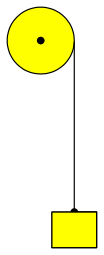
\includegraphics[ width=1.0646in, height=2.5849in,]{L4SZ281D}
}

\end {multicols}

\item [65.] A radial saw has a blade with a $6 \mbox{in}$ radius. Suppose that the blade spins at a speed
of $1000$ rpm. 

\item [(a)] Find the angular
speed of the blade in $rad/\mbox{min}\text{.}$ 

\item [(b)] Find the linear
speed of the sawteeth in $ft/\mbox{s}$. 

\item [67.] The wheels of a car have
a radius $11 \mbox{in}$ and are rotating at $600$ rpm. Find the speed of the car in $mi/\mbox{h}$. 

\item [69.] To measure the speed of
a current scientists place a paddle wheel in the stream and observe the rate at which it rotates. If the paddle
wheel has a radius $0.20 \mbox{m}$ and rotates at $100$ rpm, find the speed of the current in $\mathrm{m}/\mbox{s}$. \end{description}


%TCIMACRO{\TeXButton{Start Two Columns}{\columnsep =30pt
% \begin {multicols}{2}}}%
%BeginExpansion
\columnsep =30pt
\begin {multicols}{2}
%EndExpansion
 


%TCIMACRO{\TeXButton{End Two Columns}{\end {multicols}}}%
%BeginExpansion
\end {multicols}
%EndExpansion
 

\section{The Trigonometry of Right Triangles}


In this section we will use sine, cosine and tangent. You
should have at your fingertips the definitions of sine, cosine and tangent for a right angled triangle:
\begin{equation*}\sin  \theta  =\frac{\text{opposite}}{\text{hypotenuse}}\text{,}\cos  \theta  =\frac{\text{adjacent}}{\text{hypotenuse}}\text{and}\tan  \theta  =\frac{\text{opposite}}{\text{adjacent}}
\end{equation*}

You should be able to solve problems involving right angled triangles. A
right angled triangle is uniquely defined, if as well as the right angle, you are given two other facts about the triangle. 


\begin{enumerate}
\item Given one side and one angle 

\item Given two sides \end{enumerate}


To be given two angles does not constitute two other facts as the two angles are complementary so that given one angle the other one is known.



\begin{enumerate}
\item To solve a right triangle given one side and one angle 


\begin{description}
\item [(a)] Sketch. 

\item [(b)]
Fill in the given information and note which sides are "opp", "adj" and "hyp". 

\item [(c)]
Should the other angle be required it is found by subtraction. 

\item [(d)]
Mark the required side, pick the appropriate trigonometric ratio and solve the equation. \end{description}

\item To solve a right triangle given two sides 


\begin{description}
\item [(a)] Sketch. 

\item [(b)]
Fill in the given information. 

\item [(c)] If the third side
is required use Pythagoras theorem. 

\item [(d)] Mark the required
angle, pick the appropriate trigonometric ratio and solve the equation. (Use $\sin ^{ -1}$, $\cos ^{ -1}$ or $\tan ^{ -1}\text{.}$) \end{description}\end{enumerate}

\clearpage
\subsection{The Trigonometric Ratios of the Special Angles}
\columnsep =30pt
\begin {multicols}{2}
  
\setlength\fboxrule{0in}\setlength\fboxsep{0.2in}\fcolorbox[HTML]{000000}{FFFFFF}{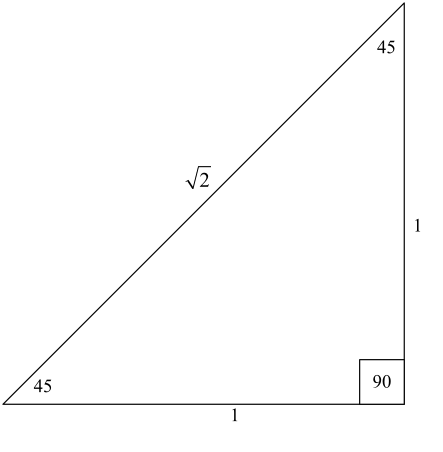
\includegraphics[ width=2.3808in, height=2.4284in,]{L4SZ281E}
}

You should be familiar with the 45, 45, 90 triangle and the ratio of the sides. Let
the two shorter sides have a length of $1$ then the hypotenuse has a length of $\sqrt{2}$. \\\relax
\begin{align*}1^{2} +1^{2} &  = 1 +1 =2 \\
\left (\sqrt{2}\right )^{2} &  = 2 \\
\text{so}1^{2} +1^{2} &  = \left (\sqrt{2}\right )^{2}\end{align*}


%TCIMACRO{\TeXButton{End Two Columns}{\end {multicols}}}%
%BeginExpansion
\end {multicols}
%EndExpansion



%TCIMACRO{\TeXButton{Start Two Columns}{\columnsep =30pt
% \begin {multicols}{2}}}%
%BeginExpansion
\columnsep =30pt
\begin {multicols}{2}
%EndExpansion
 

%   width=1.8127in, height=2.4284in,
\setlength\fboxrule{0in}\setlength\fboxsep{0.2in}\fcolorbox[HTML]{000000}{FFFFFF}{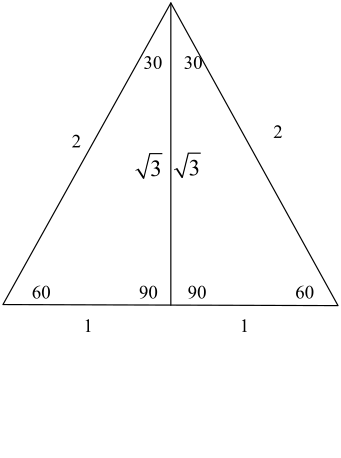
\includegraphics[ width=7cm]{L4SZ281F}
}


Similarly the equilateral triangle whose sides are 2 units gives rise to the 30, 60, 90 triangle whose sides are 1, $\sqrt{3}$ and 2. \\\relax
\begin{align*}\left (\sqrt{3}\right )^{2} +1^{2} &  =  3 +1 =4 \\
2^{2} &  =  4 \\
\text{so}\left (\sqrt{3}\right )^{2} +1^{2} &  =  2^{2}\end{align*}


\end {multicols}


The two special right triangles are the "45, 45, 90 triangle" and the "30, 60, 90 triangle". Pythagoras
theorem gives the ratio of the sides as 1, 1, $\sqrt{2}$ for the 45$\mbox{{\ensuremath{{}^\circ}}}$ 45$\mbox{{\ensuremath{{}^\circ}}}$ 90$\mbox{{\ensuremath{{}^\circ}}}$ triangle and 1, $\sqrt{3}\text{,}$ 2 for the 30$\mbox{{\ensuremath{{}^\circ}}}$ 60$\mbox{{\ensuremath{{}^\circ}}}$ 90$\mbox{{\ensuremath{{}^\circ}}}$ triangle, which is what we usually remember. 

\subsubsection{Example}
$\sin  45 \mbox{{\ensuremath{{}^\circ}}} =\frac{\text{opp}}{\text{hyp}} =\frac{1}{\sqrt{2}}$ 

We usually rationalise the denominator in expressions like $\frac{1}{\sqrt{2}}$. In other words we apply a transformation to remove the $\sqrt{2}$ from the denominator and replace it with a rational number. In this case if you multiply
the $\frac{1}{\sqrt{2}}$ by $\frac{\sqrt{2}}{\sqrt{2}}$ you get $\frac{1}{\sqrt{2}} \times \frac{\sqrt{2}}{\sqrt{2}} =\frac{\sqrt{2}}{2}$. 

Another way to achieve this is to start with the triangle 


%TCIMACRO{\TeXButton{Start Two Columns}{\columnsep =30pt
% \begin {multicols}{2}}}%
%BeginExpansion
\columnsep =30pt
\begin {multicols}{2}
%EndExpansion
 

   
\setlength\fboxrule{0in}\setlength\fboxsep{0.2in}\fcolorbox[HTML]{000000}{FFFFFF}{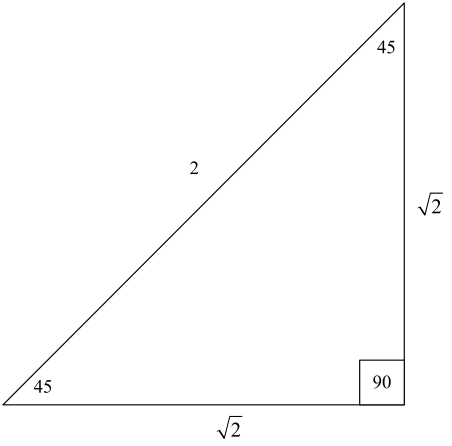
\includegraphics[ width=2.4639in, height=2.4284in,]{L4SZ281G}
}


By Pythagoras theorem
\begin{equation*}\left (\sqrt{2}\right )^{2} +\left (\sqrt{2}\right )^{2} =2 +2 =4 =2^{2}
\end{equation*}


%TCIMACRO{\TeXButton{End Two Columns}{\end {multicols}}}%
%BeginExpansion
\end {multicols}
%EndExpansion
\begin{equation*}\text{So}\sin  45 \mbox{{\ensuremath{{}^\circ}}} =\frac{\sqrt{2}}{2}\text{,}\cos  45 \mbox{{\ensuremath{{}^\circ}}} =\frac{\sqrt{2}}{2}\text{and}\tan  45 \mbox{{\ensuremath{{}^\circ}}} =\frac{\sqrt{2}}{\sqrt{2}} =1
\end{equation*}

If you are asked for the exact values of $\sin  45 \mbox{{\ensuremath{{}^\circ}}}$, $\cos  45 \mbox{{\ensuremath{{}^\circ}}}$ or $\tan  45 \mbox{{\ensuremath{{}^\circ}}}$ you should give these results. 

From the 30, 60, 90 triangle
\begin{align*}\sin  30 \mbox{{\ensuremath{{}^\circ}}} &  =  \frac{1}{2}\text{,}\cos  30 \mbox{{\ensuremath{{}^\circ}}} =\frac{\sqrt{3}}{2}\text{and}\tan  30 \mbox{{\ensuremath{{}^\circ}}} =\frac{1}{\sqrt{3}} =\frac{\sqrt{3}}{3} \\
\sin  60 \mbox{{\ensuremath{{}^\circ}}} &  = \frac{\sqrt{3}}{2}\text{,}\cos  60 \mbox{{\ensuremath{{}^\circ}}} =\frac{1}{2}\text{and}\tan  60 \mbox{{\ensuremath{{}^\circ}}} =\frac{\sqrt{3}}{1} =\sqrt{3}\end{align*}

\subsection{The Relationship between Degrees and Radians for the \\ Special Right Triangles}

\begin{align*}\sin  \frac{\pi }{4} &  =  \frac{\sqrt{2}}{2}\text{,}\cos  \frac{\pi }{4} =\frac{\sqrt{2}}{2}\text{and}\tan  \frac{\pi }{4} =\frac{\sqrt{2}}{\sqrt{2}} =1 \\
\text{So}\frac{\pi }{4} &  =  45 \mbox{{\ensuremath{{}^\circ}}}\end{align*}


\begin{align*}\sin  \frac{\pi }{6} &  =  \frac{1}{2}\text{,}\cos  \frac{\pi }{6} =\frac{\sqrt{3}}{2}\text{and}\tan  \frac{\pi }{6} =\frac{1}{\sqrt{3}} =\frac{\sqrt{3}}{3} \\
\text{So}\frac{\pi }{6} &  =  30 \mbox{{\ensuremath{{}^\circ}}}\end{align*}
\begin{align*}\sin  \frac{\pi }{3} &  =  \frac{\sqrt{3}}{2}\text{,}\cos  \frac{\pi }{3} =\frac{1}{2}\text{and}\tan  \frac{\pi }{3} =\frac{\sqrt{3}}{1} =\sqrt{3} \\
\text{So}\frac{\pi }{3} &  =  60 \mbox{{\ensuremath{{}^\circ}}}\end{align*}

The calculator gives approximate values of the trigonometric ratios. You
must look at your question to check whether angles are in degrees or radians and ensure the calculator is first set in the right \emph{mode}.
\ Remember all questions where degrees are to be used will give angles marked with a $\mbox{{\ensuremath{{}^\circ}}}$ symbol. You could assume though that when you
are dealing with a static problem (i.e. one where a triangle is given and sides and angles are required) then the angle will be measured in degrees. 

When you are required to find a side you select the trigonometric ratio and either multiply or divide.
\ When you are required to find an angle you select the appropriate trigonometry ratio and use \emph{shift}
with sin, cos or tan to find $\sin ^{ -1}$, $\cos ^{ -1}$ or $\tan ^{ -1}$ because $\sin ^{ -1}$ is said "the angle whose sine is" etc. 

\subsection{Applications}
 

\subsubsection{Example 1}
The height of a steep cliff is to be measured from a point on the opposite side of the river.  The
following diagram shows the measurements taken. Estimate the height of the cliff. 


%TCIMACRO{\TeXButton{Start Two Columns}{\columnsep =30pt
% \begin {multicols}{2}}}%
%BeginExpansion
\columnsep =30pt
\begin {multicols}{2}
%EndExpansion
 

   
\setlength\fboxrule{0in}\setlength\fboxsep{0.2in}\fcolorbox[HTML]{000000}{FFFFFF}{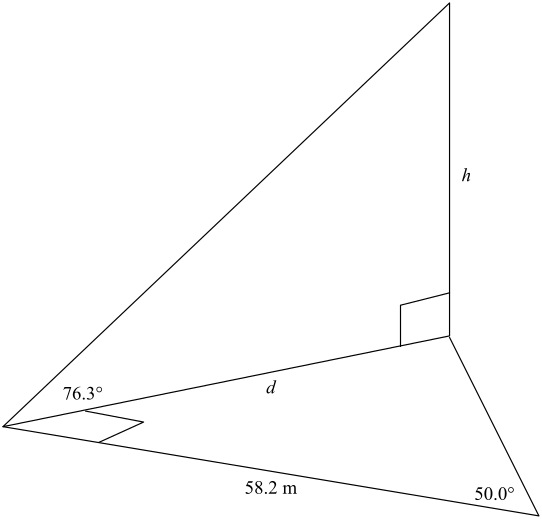
\includegraphics[ width=9cm]{L4SZ281H}
}



\begin{align*}\frac{d}{58.2} &  =  \tan  50.0 \mbox{{\ensuremath{{}^\circ}}} \\
d &  =  58.2 \times \tan  50.0 \mbox{{\ensuremath{{}^\circ}}} \\
\frac{h}{d} &  =  \tan  76.3 \mbox{{\ensuremath{{}^\circ}}} \\
h &  =  d \times \tan  76.3 \mbox{{\ensuremath{{}^\circ}}} \\
 &  =  58.2 \times \tan  50.0 \mbox{{\ensuremath{{}^\circ}}} \times \tan  76.3 \mbox{{\ensuremath{{}^\circ}}} \\
 &  \approx   284.526397 \\
 &  \approx   284.5 \mbox{m}\end{align*}


%TCIMACRO{\TeXButton{End Two Columns}{\end {multicols}}}%
%BeginExpansion
\end {multicols}
%EndExpansion


\subsubsection{Example 2}
To estimate the height of a mountain above a level plane the angle of elevation of the top of the mountain is measured to be $30 \mbox{{\ensuremath{{}^\circ}}}$. $600 \mbox{m}$ closer to the mountain across the plane it is found that the angle of elevation
is $36 \mbox{{\ensuremath{{}^\circ}}}$. Estimate the height of the mountain. 

   
\setlength\fboxrule{0in}\setlength\fboxsep{0.2in}\fcolorbox[HTML]{000000}{FFFFFF}{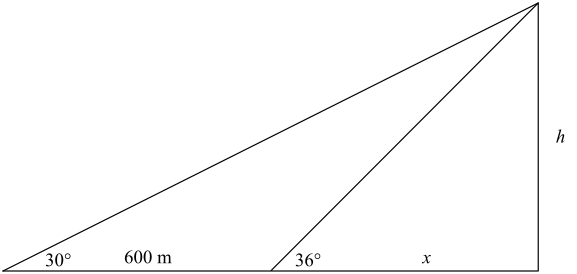
\includegraphics[ width=12cm]{L4SZ281I}
}


\begin{equation*}\frac{h}{x} =\tan  36 \mbox{{\ensuremath{{}^\circ}}}\text{and}\frac{h}{x +600} =\tan  30 \mbox{{\ensuremath{{}^\circ}}}
\end{equation*}

We want $h$ so we eliminate $x$ between these two equations
\begin{align*}x &  =  \frac{h}{\tan  36 \mbox{{\ensuremath{{}^\circ}}}}\text{and}x +600 =\frac{h}{\tan  30 \mbox{{\ensuremath{{}^\circ}}}} \\
\frac{h}{\tan  30 \mbox{{\ensuremath{{}^\circ}}}} &  =  \frac{h}{\tan  36 \mbox{{\ensuremath{{}^\circ}}}} +600 \\
\frac{h}{\tan  30 \mbox{{\ensuremath{{}^\circ}}}} -\frac{h}{\tan  36 \mbox{{\ensuremath{{}^\circ}}}} &  =  600 \\
h \left (\frac{1}{\tan  30 \mbox{{\ensuremath{{}^\circ}}}} -\frac{1}{\tan  36 \mbox{{\ensuremath{{}^\circ}}}}\right ) &  =  600 \\
h \genfrac{(}{)}{}{}{\tan  36 \mbox{{\ensuremath{{}^\circ}}} -\tan  30 \mbox{{\ensuremath{{}^\circ}}}}{\tan  30 \mbox{{\ensuremath{{}^\circ}}} \tan  36 \mbox{{\ensuremath{{}^\circ}}}} &  =  600 \\
h &  =  600 \times \frac{\tan  30 \mbox{{\ensuremath{{}^\circ}}} \tan  36 \mbox{{\ensuremath{{}^\circ}}}}{\tan  36 \mbox{{\ensuremath{{}^\circ}}} -\tan  30 \mbox{{\ensuremath{{}^\circ}}}} \\
 &  \approx   600 \times 2.811603815 \\
 &  \approx   1687 \mbox{m}\end{align*}
\clearpage
\subsubsection{Example 3}
Now use the same method to show that for 
  
\setlength\fboxrule{0in}\setlength\fboxsep{0.2in}\fcolorbox[HTML]{000000}{FFFFFF}{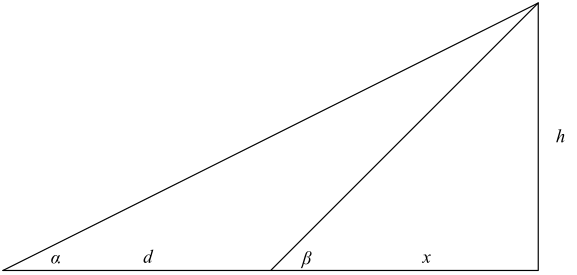
\includegraphics[ width=12cm]{L4SZ281J}
}
\begin{equation*}h =d \frac{\tan  \alpha  \tan  \beta }{\tan  \beta  -\tan  \alpha }
\end{equation*}

Let $x$ be the distance shown on the diagram.
\begin{align*}\frac{h}{x} &  =  \tan  \beta \text{and}\frac{h}{x +d} =\tan  \alpha  \\
\text{So}x &  =  \frac{h}{\tan  \beta }\text{and}x +d =\frac{h}{\tan  \alpha } \\
\text{Then}\frac{h}{\tan  \beta } +d &  =  \frac{h}{\tan  \alpha } \\
\frac{h}{\tan  \alpha } -\frac{h}{\tan  \beta } &  =  d \\
h \left (\frac{1}{\tan  \alpha } -\frac{1}{\tan  \beta }\right ) &  =  d \\
h \genfrac{(}{)}{}{}{\tan  \beta  -\tan  \alpha }{\tan  \alpha  \tan  \beta } &  =  d \\
h &  =  d \frac{\tan  \alpha  \tan  \beta }{\tan  \beta  -\tan  \alpha }\end{align*}

\subsection{Exercises}

\begin{description}
\item [1.]  Find the exact value of $\sin  \theta $, $\cos  \theta $ and $\tan  \theta $ of the angle $\theta $ in the triangle. \\
 
\columnsep =30pt
\begin {multicols}{2}  
\setlength\fboxrule{0in}\setlength\fboxsep{0.2in}\fcolorbox[HTML]{000000}{FFFFFF}{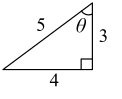
\includegraphics[ width=1.1632in, height=0.9548in,]{L4SZ281K}
}


\item [3.]  Find the angle $\theta$  
\setlength\fboxrule{0in}\setlength\fboxsep{0.2in}\fcolorbox[HTML]{000000}{FFFFFF}{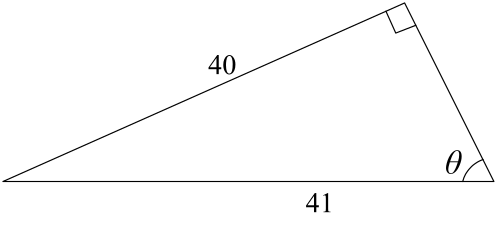
\includegraphics[ width=2.8003in, height=1.2756in,]{L4SZ281L}
}
%TCIMACRO{\TeXButton{End Two Columns}{\end {multicols}}}%
%BeginExpansion
\end {multicols}
%EndExpansion
 

\item [5.] Find the angle $\theta$
\setlength\fboxrule{0in}\setlength\fboxsep{0.2in}\fcolorbox[HTML]{000000}{FFFFFF}{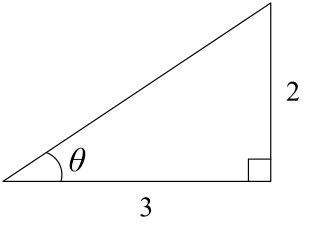
\includegraphics[ width=1.9562in, height=1.3932in,]{L4SZ281M}
}
\end{description}

Find the side labelled x. 


\begin{description}
\item [10.]   
%TCIMACRO{\TeXButton{Start Two Columns}{\columnsep =30pt
% \begin {multicols}{2}}}%
%BeginExpansion
\columnsep =30pt
\begin {multicols}{2}
%EndExpansion
    
\setlength\fboxrule{0in}\setlength\fboxsep{0.2in}\fcolorbox[HTML]{000000}{FFFFFF}{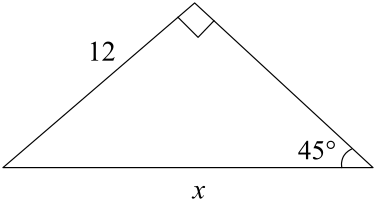
\includegraphics[ width=2.1698in, height=1.2254in,]{L4SZ281N}
}


\item [11.]    
\setlength\fboxrule{0in}\setlength\fboxsep{0.2in}\fcolorbox[HTML]{000000}{FFFFFF}{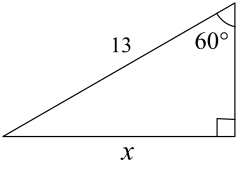
\includegraphics[ width=1.7348in, height=1.2462in,]{L4SZ281O}
}
%TCIMACRO{\TeXButton{End Two Columns}{\end {multicols}}}%
%BeginExpansion
\end {multicols}
%EndExpansion
 

\item [13.]
\setlength\fboxrule{0in}\setlength\fboxsep{0.2in}\fcolorbox[HTML]{000000}{FFFFFF}{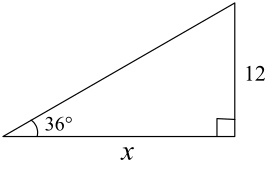
\includegraphics[ width=1.996in, height=1.2289in,]{L4SZ281P}
}
\end{description}




\begin{description}
\item [29.]   Solve the triangle 
%TCIMACRO{\TeXButton{Start Two Columns}{\columnsep =30pt
% \begin {multicols}{2}}}%
%BeginExpansion
\columnsep =30pt
\begin {multicols}{2}
%EndExpansion
    
\setlength\fboxrule{0in}\setlength\fboxsep{0.2in}\fcolorbox[HTML]{000000}{FFFFFF}{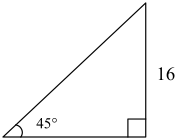
\includegraphics[ width=2.0055in, height=1.4909in,]{L4SZ281Q}
}


\item [31.]    Solve the triangle 
\setlength\fboxrule{0in}\setlength\fboxsep{0.2in}\fcolorbox[HTML]{000000}{FFFFFF}{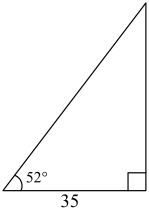
\includegraphics[ width=1.5843in, height=2.3065in,]{L4SZ281R}
}
%TCIMACRO{\TeXButton{End Two Columns}{\end {multicols}}}%
%BeginExpansion
\end {multicols}
%EndExpansion
 

\item [35.]
The angle of elevation to the top of the Empire State Building in New York is found to be $11 \mbox{{\ensuremath{{}^\circ}}}$ from the ground at a distance of $1 \mbox{mi}$ from the base of the building. Using this information,
find the height of the Empire State Building. 

\item [35.]
A laser beam is to be directed towards the centre of the moon but the beam strays $0.5 \mbox{{\ensuremath{{}^\circ}}}$ from its intended path. 

\item [(a)]
How far has the beam diverged from its assigned target when it reaches the moon? (The distance of the earth
to the moon is $240$ $000 \mbox{mi}\text{.}$) 

\item [(b)] The radius
of the moon is about $1000 \mbox{mi}$. Will the beam strike the moon? 

\item [39.]
A $20 \mbox{ft}$ ladder leans against a building so that the angle between the ground and the ladder is $72 \mbox{{\ensuremath{{}^\circ}}}$. How high does the ladder reach on the building?


\item [42.] A $96 \mbox{ft}$ tree casts a shadow that is $120 \mbox{ft}$ long. What is the angle of elevation of the sun?


\item [43.] a man is lying on the beach, flying a kite. He
holds the end of the kite string at ground level, and estimates that the angle of elevation of the kite to be $50 \mbox{{\ensuremath{{}^\circ}}}$. If the string is $450 \mbox{ft}$ long, how high is the kite above the ground? 

\item [45.]
A water tower is located $325 \mbox{ft}$ from a building. From a window in the building
it is observed that the angle of elevation to the top of the tower is $39 \mbox{{\ensuremath{{}^\circ}}}$ and the angle of depression to the bottom of the tower is $25 \mbox{{\ensuremath{{}^\circ}}}$. How tall is the tower? How
high is the window? 

\item [46.] An airplane is flying at an
elevation of $5150 \mbox{ft}$ directly above a straight highway. Two motorists
are driving cars on the highway on opposite sides of the plane and the angle of depression to one car is $35 \mbox{{\ensuremath{{}^\circ}}}$ and to the other is $52 \mbox{{\ensuremath{{}^\circ}}}$. How far apart are the cars? 

\item [49.]
To estimate the height of a mountain above a level plain, the angle of elevation to the top of the mountain is measured to be $32 \mbox{{\ensuremath{{}^\circ}}}$. One thousand feet closed to the mountain along
the plain, it is found that the angle of elevation is $35 \mbox{{\ensuremath{{}^\circ}}}$. Estimate the height of the mountain. \end{description}

 

\section{The Trigonometric Functions of Angles}


In the previous section the angles were between $0 \mbox{{\ensuremath{{}^\circ}}}$ and $90 \mbox{{\ensuremath{{}^\circ}}}$. In this section the angles can take any value.
\ Initially we consider angles between $0 \mbox{{\ensuremath{{}^\circ}}}$ and $360 \mbox{{\ensuremath{{}^\circ}}}$ and relate these to the radian measure between $0$ and $2 \pi $. We remind you that angles are measured anticlockwise from the positive $x$-axis. 

If the point $P (x ,y)$ is in the first quadrant, $\theta $ is the angle between $OP$ and the positive $x$-axis and we complete the right triangle then we have created the following situation.  
%TCIMACRO{\TeXButton{Start Two Columns}{\columnsep =30pt
% \begin {multicols}{2}}}%
%BeginExpansion
\columnsep =30pt
\begin {multicols}{2}
%EndExpansion
 

   
\setlength\fboxrule{0in}\setlength\fboxsep{0.2in}\fcolorbox[HTML]{000000}{FFFFFF}{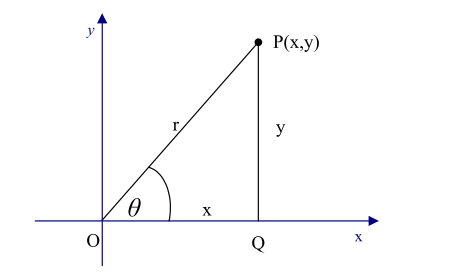
\includegraphics[ width=3.774in, height=2.3454in,]{L4SZ281S}
}


Let the hypotenuse be $r$ then
\begin{equation*}r =\sqrt{x^{2} +y^{2}}
\end{equation*}


%TCIMACRO{\TeXButton{End Two Columns}{\end {multicols}}}%
%BeginExpansion
\end {multicols}
%EndExpansion


Therefore
\begin{equation*}\sin  \theta  =\frac{y}{r}\text{}\cos  \theta  =\frac{x}{r}\text{and}\tan  \theta  =\frac{y}{x}
\end{equation*}

We now let $\theta $ be any angle and define sine, cosine and tangent in the same way. For instance
if $P (x ,y)$ is in the second quadrant: 

   
\setlength\fboxrule{0in}\setlength\fboxsep{0.2in}\fcolorbox[HTML]{000000}{FFFFFF}{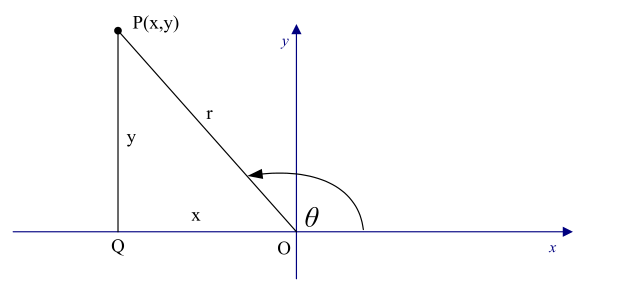
\includegraphics[ width=3.9868in, height=1.8161in,]{L4SZ281T}
}


$\sin  \theta  =\frac{y}{r}$ because $y$ is positive $\sin  \theta $ will be positive. ($r$ is positive by convention.) 

$\cos  \theta  =\frac{x}{r}$ because $x$ is negative $\cos  \theta $ will be negative. 

$\tan  \theta  =\frac{y}{x}$ because $y$ is positive and $x$ is negative $\tan  \theta $ will be negative. 

This pattern can be extended to quadrants 3 and 4. The
mnemonic (\textbf{A}ll \textbf{S}tudents \textbf{T}ake \textbf{C}alculus) might help you remember which one is positive
although you can always work it out if you need to. 

%\subsection{Relating Angles between 0$\mbox{{\ensuremath{{}^\circ}}}$ and 360$\mbox{{\ensuremath{{}^\circ}}}$ to an Equivalent Angle between 0$\mbox{{\ensuremath{{}^\circ}}}$ and 90$\mbox{{\ensuremath{{}^\circ}}}$}
%By constructing $\bar{PQ}$ perpendicular to the $x$-axis a triangle is formed and this can be transformed into a congruent triangle in the first quadrant.This
%is particularly important if an exact value is required for one of the special angles. 
%
%\subsubsection{Example 1}
%Given $\sin  60 \mbox{{\ensuremath{{}^\circ}}} =\frac{\sqrt{3}}{2}$ it can be shown $\sin  120 \mbox{{\ensuremath{{}^\circ}}} =\frac{\sqrt{3}}{2}$, $\sin  240 \mbox{{\ensuremath{{}^\circ}}} = -\frac{\sqrt{3}}{2}$ and $\sin  300 \mbox{{\ensuremath{{}^\circ}}} = -\frac{\sqrt{3}}{2}$ 
%
%\subsubsection{Example 2}
%Given $\cos  45 \mbox{{\ensuremath{{}^\circ}}} =\frac{\sqrt{2}}{2}$ it can be shown $\cos  135 \mbox{{\ensuremath{{}^\circ}}} = -\frac{\sqrt{2}}{2}$, $\cos  225 \mbox{{\ensuremath{{}^\circ}}} = -\frac{\sqrt{2}}{2}$ and $\cos  315 \mbox{{\ensuremath{{}^\circ}}} =\frac{\sqrt{2}}{2}$ 
%
%This can be continued beyond $360 \mbox{{\ensuremath{{}^\circ}}}$. 
%
%\subsubsection{Example 3}
%Given $\tan  30 \mbox{{\ensuremath{{}^\circ}}} =\frac{\sqrt{3}}{3}$ it can be shown $\tan  390 \mbox{{\ensuremath{{}^\circ}}} =\frac{\sqrt{3}}{3}$, $\tan  510 \mbox{{\ensuremath{{}^\circ}}} = -\frac{\sqrt{3}}{3}$, $\tan  570 \mbox{{\ensuremath{{}^\circ}}} =\frac{\sqrt{3}}{3}$ and $\tan  690 \mbox{{\ensuremath{{}^\circ}}} = -\frac{\sqrt{3}}{3}$ 
%
%This also holds for angles measured in a clockwise direction 
%
%\subsubsection{Example 4}
%Given $\tan  45 \mbox{{\ensuremath{{}^\circ}}} =1$ it can be shown $\tan  -45 \mbox{{\ensuremath{{}^\circ}}} = -1$, $\tan  -135 \mbox{{\ensuremath{{}^\circ}}} = -1$, $\tan  -225 \mbox{{\ensuremath{{}^\circ}}} = -1$ and $\tan  -315 \mbox{{\ensuremath{{}^\circ}}} =1$ 
%
%The textbook refers to this as finding the \emph{reference angle}. We
%will avoid this additional definition, however the procedure of finding the congruent triangle in the first quadrant must be understood. Although
%the same logic can be applied to \emph{any} angle in that a congruent triangle can be constructed in the first quadrant we will only bother
%to do this for the special angles. For all other angles the calculator gives an approximate value. You
%should note therefore whether a special angle is given where an exact answer is expected or whether an approximate answer will suffice. 

\subsection{The Area of a Triangle}
The fundamental formula for the area of a triangle is
\begin{equation*}\text{Area} =\frac{1}{2} \times \text{base} \times \text{height}
\end{equation*}

Using the trigonometric functions the height can be replaced
and the formula becomes
\begin{equation*}\text{Area} =\frac{1}{2} \times \text{product of two sides} \times \text{sine of the included angle}
\end{equation*}

The formula is particularly easy to remember in symbolic form. Let
the triangle have vertices $A$, $B$ and $C$, so the the sides opposite these angles are $a$, $b$ and $c$ respectively. Then the area can be expressed symbolically as
\begin{equation*}\text{Area} =\frac{1}{2} a b \sin  C =\frac{1}{2} b c \sin  A =\frac{1}{2} a c \sin  B
\end{equation*}


%TCIMACRO{\TeXButton{Start Two Columns}{\columnsep =30pt
% \begin {multicols}{2}}}%
%BeginExpansion
\columnsep =30pt
\begin {multicols}{2}
%EndExpansion
 

   
\setlength\fboxrule{0in}\setlength\fboxsep{0.2in}\fcolorbox[HTML]{000000}{FFFFFF}{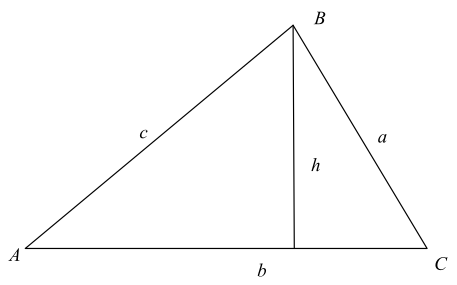
\includegraphics[ width=3.1012in, height=1.9415in,]{L4SZ281U}
}



\begin{align*}\sin  A &  = \frac{h}{c}\text{so}h =c \sin  A \\
\text{Area} &  =  \frac{1}{2} \times \text{base} \times \text{height} \\
 &  =  \frac{1}{2} \times b \times c \sin  A =\frac{1}{2} b c \sin  A\end{align*}


%TCIMACRO{\TeXButton{End Two Columns}{\end {multicols}}}%
%BeginExpansion
\end {multicols}
%EndExpansion


It depends where you draw $h$ and which angle you choose to use as to which formula you finish up with. The key
point to remember is $b$ and $c$ are two sides and $A$ is the angle between them. The triangle above shows $A$ as an acute angle (between $0$ and $90 \mbox{{\ensuremath{{}^\circ}}}$). If the angle is obtuse (between $90 \mbox{{\ensuremath{{}^\circ}}}$ and $180 \mbox{{\ensuremath{{}^\circ}}}$) the formula still holds. 

   
\setlength\fboxrule{0in}\setlength\fboxsep{0.2in}\fcolorbox[HTML]{000000}{FFFFFF}{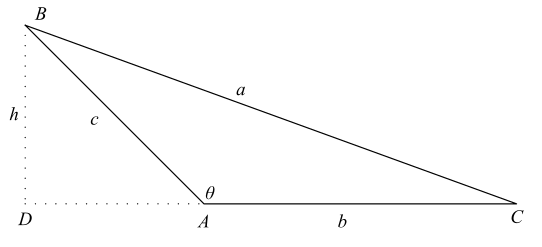
\includegraphics[ width=3.6573in, height=1.6769in,]{L4SZ281V}
}


The angle is in the second quadrant and $\sin  (180 -\theta ) =\sin  \theta $, so $\sin  (180 -\theta ) =\frac{h}{c}$ can be written as $\sin  \theta  =\frac{h}{c}$ or $h =c \sin  \theta $ or $h =c \sin  A$ where $A$ is obtuse. So the area is $\frac{1}{2} b c \sin  A$ 

\subsubsection{Example 5}
A triangle has two sides of $5 \mbox{cm}$ and $8 \mbox{cm}$ and the angle between them is $150 \mbox{{\ensuremath{{}^\circ}}}$. Find its area.
\begin{equation*}\text{Area} =\frac{1}{2} \times 5 \times 8 \times \sin  150 \mbox{{\ensuremath{{}^\circ}}}
\end{equation*}

It helps to remember that $\sin  150 =\sin  30 =\frac{1}{2}$
\begin{equation*}\text{Area} =\frac{1}{2} \times 5 \times 8 \times \frac{1}{2} =10 cm^{2}
\end{equation*}

\subsection{Exercises}
Find the exact value of the trigonometric function
\begin{description}
\item [7.]   
%TCIMACRO{\TeXButton{Start Two Columns}{\columnsep =30pt
% \begin {multicols}{2}}}%
%BeginExpansion
\columnsep =30pt
\begin {multicols}{2}
%EndExpansion
 $\sin  150 \mbox{{\ensuremath{{}^\circ}}}$ 

\item [9.] $\cos  135 \mbox{{\ensuremath{{}^\circ}}}$ 
%TCIMACRO{\TeXButton{End Two Columns}{\end {multicols}}}%
%BeginExpansion
\end {multicols}
%EndExpansion
 

\item [11.]
%TCIMACRO{\TeXButton{Start Two Columns}{\columnsep =30pt
% \begin {multicols}{2}}}%
%BeginExpansion
\columnsep =30pt
\begin {multicols}{2}
%EndExpansion
 $\tan  \left ( -60 \mbox{{\ensuremath{{}^\circ}}}\right )$ 

\item [15.] $\cos  570 \mbox{{\ensuremath{{}^\circ}}}$ 
%TCIMACRO{\TeXButton{End Two Columns}{\end {multicols}}}%
%BeginExpansion
\end {multicols}
%EndExpansion
  

\item [17.]   
%TCIMACRO{\TeXButton{Start Two Columns}{\columnsep =30pt
% \begin {multicols}{2}}}%
%BeginExpansion
\columnsep =30pt
\begin {multicols}{2}
%EndExpansion
 $\tan  750 \mbox{{\ensuremath{{}^\circ}}}$ 

\item [19.] $\sin  \frac{2 \pi }{3}$ 
%TCIMACRO{\TeXButton{End Two Columns}{\end {multicols}}}%
%BeginExpansion
\end {multicols}
%EndExpansion
 

\item [21.]
%TCIMACRO{\TeXButton{Start Two Columns}{\columnsep =30pt
% \begin {multicols}{2}}}%
%BeginExpansion
\columnsep =30pt
\begin {multicols}{2}
%EndExpansion
 $\sin  \frac{3 \pi }{2}$ 

\item [23.] $\cos  \left ( -\frac{7 \pi }{3}\right )$ 
%TCIMACRO{\TeXButton{End Two Columns}{\end {multicols}}}%
%BeginExpansion
\end {multicols}
%EndExpansion
 

\item [29.]
$\tan  \frac{5 \pi }{2}$ \end{description}

Find the value of the trigonometric functions of $\theta $ from the information given 


\begin{description}
\item [41.] $\sin  \theta  =\frac{3}{5}\text{,}$ $\theta $ in quadrant II 

\item [43.]
$\tan  \theta  = -\frac{3}{4}\text{,}$ $\cos  \theta  >0$ 

\item [49.] If $\theta  =\pi /3\text{,}$ find the value of each expression. 

\item [(a)]
%TCIMACRO{\TeXButton{Start Two Columns}{\columnsep =30pt
% \begin {multicols}{2}}}%
%BeginExpansion
\columnsep =30pt
\begin {multicols}{2}
%EndExpansion
 $\sin  2 \theta \text{,}$ $2 \sin  \theta $ 

\item [(b)] $\sin  \frac{1}{2} \theta \text{,}$ $\frac{\sin  \theta }{2}$ 
%TCIMACRO{\TeXButton{End Two Columns}{\end {multicols}}}%
%BeginExpansion
\end {multicols}
%EndExpansion
 

\item [(c)]
$\sin ^{2} \theta \text{,}$ $\sin  \left (\theta ^{2}\right )$ 

\item [51.] Find the area of a triangle
with sides of length $7$ and $9$ and included angle $72 \mbox{{\ensuremath{{}^\circ}}}$. 

\item [53.]
A triangle has an area of $16 in^{2}\text{,}$ and two of the sides of the triangle have lengths $5 \mbox{in}$ and $7 \mbox{in}$. Find the angle included by these two sides. \end{description}


%TCIMACRO{\TeXButton{Start Two Columns}{\columnsep =30pt
% \begin {multicols}{2}}}%
%BeginExpansion
\columnsep =30pt
\begin {multicols}{2}
%EndExpansion
 


%TCIMACRO{\TeXButton{End Two Columns}{\end {multicols}}}%
%BeginExpansion
\end {multicols}
%EndExpansion
 

\section{The Sine Rule}


In this section we use the Sine Rule to find the sides and angles in triangles without a right angle.
\ In the next section we use the Cosine Rule to find sides and angles in triangles also, so as you study these
two sections you need to learn which problems require the Sine Rule and which require the Cosine Rule. 

Previously, we met the formula
for the area of a triangle. given two sides and the included angle $\left ( =\frac{1}{2} a b \sin  C\right )$. The Sine Rule and
Cosine Rule also require specific combinations of sides and angles. 

The easiest way to visualise the situations in which the two rules
are used is to use the labelling we met in section $3.3$. Let the triangle be $ \Delta A B C$ and let the sides be $a$, $b$ and $c$ where $a$ is opposite $\angle A$ etc. 

   
\setlength\fboxrule{0in}\setlength\fboxsep{0.2in}\fcolorbox[HTML]{000000}{FFFFFF}{
\includegraphics[ width=3.1358in, height=2.4171in,]{L4SZ281W}
}



\begin{tabular}[c]{lll}\textbf{Sine Rule}  &  & \textbf{Cosine
Rule}  \\
 Given a side and the angle opposite the side  &  & \textbf{(a)}
Given two sides and the included angle  \\
 \textbf{(a)} If a second angle is
given the Sine Rule  &  & the Cosine Rule allows us to find the
side  \\
allows us the side opposite that angle  &  & opposite
the angle  \\
Given $A$, $a$ and $B$ use the Sine Rule to find $b\text{.}$  &  & Given $a$, $b$ and $C$ use the Cosine Rule to find $c\text{.}$  \\
 \textbf{(b)} If a second
angle is given and the side that  &  & \textbf{(b)} Given three
sides the Cosine Rule allows  \\
is not opposite that angle is required then first  &  & us
to find any angle.  \\
find the third angle then use (a).  &  & Given
$a$, $b$ and $c$ use the Cosine Rule to find $A$  \\
Given $A$, $a$ and $B$ where $c$ is required  &  & or $B$ or $C$.  \\
 1. $C =180 -(A +B)$  &  &  \\
2.
Use the Sine Rule to find $c$.  &  &  \\
\textbf{(c)} If a second side is given the Sine Rule  &  &  \\
allows
us to find the angle opposite that side.  &  &  \\
Given
$A$, $a$, and $b$ use the Sine Rule to find $B$.  &  &  \\
\end{tabular}

Textbooks may use the term ``The Law of Sines" whereas in these notes the term
``The Sine Rule will be used. 

The Sine Rule states that in any triangle
\begin{equation*}\frac{\sin  A}{a} =\frac{\sin  B}{b} =\frac{\sin  C}{c}
\end{equation*}

or
\begin{equation*}\frac{a}{\sin  A} =\frac{b}{\sin  B} =\frac{c}{\sin  C}
\end{equation*}

\subsection{Proof of the Sine Rule}
The Sine Rule is easy to prove from the formula for the area of a triangle
\begin{equation*}\text{Area} =\frac{1}{2} b c \sin  A =\frac{1}{2} a c \sin  B =\frac{1}{2} a b \sin  C
\end{equation*}

Multiply right through by 2
\begin{equation*}b c \sin  A =a c \sin  B =a b \sin  C
\end{equation*}

Divide right through by $a b c$
\begin{equation*}\frac{\sin  A}{a} =\frac{\sin  B}{b} =\frac{\sin  C}{c}
\end{equation*}

Fractions can always be inverted as long as the same process is applied to each fraction.
\begin{equation*}\frac{a}{\sin  A} =\frac{b}{\sin  B} =\frac{c}{\sin  C}
\end{equation*}

\subsubsection{Example 1}
   
\setlength\fboxrule{0in}\setlength\fboxsep{0.2in}\fcolorbox[HTML]{000000}{FFFFFF}{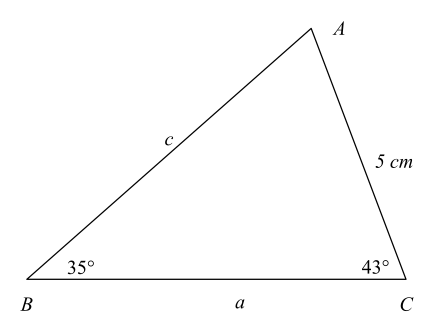
\includegraphics[ width=2.6143in, height=2.0159in,]{L4SZ281X}
}
\\\relax (a) To find $c$
\begin{align*}\frac{c}{\sin  C} &  = \frac{b}{\sin  B} \\
\frac{c}{\sin  43 \mbox{{\ensuremath{{}^\circ}}}} &  = \frac{5}{\sin  35 \mbox{{\ensuremath{{}^\circ}}}} \\
c &  = \frac{5 \sin  43 \mbox{{\ensuremath{{}^\circ}}}}{\sin  35 \mbox{{\ensuremath{{}^\circ}}}} \\
 &  \approx   5.945139277 \approx 5.9 \mbox{cm}\text{(1 dp)}\end{align*} \\\relax (b) To find $a$ 

(i) $A =180 \mbox{{\ensuremath{{}^\circ}}} -(35 \mbox{{\ensuremath{{}^\circ}}} +43 \mbox{{\ensuremath{{}^\circ}}}) =180 \mbox{{\ensuremath{{}^\circ}}} -78 \mbox{{\ensuremath{{}^\circ}}} =102 \mbox{{\ensuremath{{}^\circ}}}$ 

(ii) It is usually wise to go back to the original data (i.e. use $b$ and $B$ rather than $c$ and $C$).
\begin{align*}\frac{a}{\sin  A} &  = \frac{b}{\sin  B} \\
\frac{a}{\sin  102 \mbox{{\ensuremath{{}^\circ}}}} &  = \frac{5}{\sin  35 \mbox{{\ensuremath{{}^\circ}}}} \\
a &  = \frac{5 \sin  102 \mbox{{\ensuremath{{}^\circ}}}}{\sin  35 \mbox{{\ensuremath{{}^\circ}}}} \\
 &  \approx   8.526741501 \approx 8.5 \mbox{cm}\text{(1 dp)}\end{align*}

These two calculations
illustrate the first two cases in which the Sine Rule is used. You will notice that the triangle has been completely
solved in the course of this example. We started with one side and two angles and we found the other two sides
and the other angle. 

The third case is not as straight forward. Given two sides and an
angle there could be no triangle formed, one triangle formed or two triangles formed depending on the length of the side opposite the given angle. You should develop an insight into the reasons why
this is so. Imagine the second side given is the boom of a crane and the angle given is the angle between the
boom and the ground. The side opposite the given angle is represented by the cable. It is clear that for certain
lengths of the cable the hook will not reach the ground. Then as the hook is lowered a point will be reached
when the hook just touches the ground.  
%TCIMACRO{\TeXButton{Start Two Columns}{\columnsep =30pt
% \begin {multicols}{2}}}%
%BeginExpansion
\columnsep =30pt
\begin {multicols}{2}
%EndExpansion
 

   
\setlength\fboxrule{0in}\setlength\fboxsep{0.2in}\fcolorbox[HTML]{000000}{FFFFFF}{
\includegraphics[ width=2.9577in, height=2.2061in,]{L4SZ281Y}
}


It is no surprise that the length $a$ to create this situation is $a =b \sin  A\text{.}$ 

We are after all dealing with the Sine Rule which becomes the fundamental sine formula $\left (\sin  A =\frac{\text{opp}}{\text{hyp}} =\frac{a}{b}\right )$ when the triangle has a right angle. 
%TCIMACRO{\TeXButton{End Two Columns}{\end {multicols}}}%
%BeginExpansion
\end {multicols}
%EndExpansion


If the cable is held taut and is extended a little more it will touch the ground in two places (provided it is kept in the same plane).
\ As the cable is extended further the time will come where the cable is as long as boom. At
this point there is only one solution again, the one straight out in front of the crane). Further extensions
of the cable will produce only one solution (straight out in front of the crane) as the cable will theoretically reach behind the crane boom thus creating
a different triangle altogether. 

The two solutions case is often referred to as the ambiguous case. The
discussion above shows the range of values of $a$ that will give two solutions.
\begin{equation*}b \sin  A <a <b
\end{equation*}

\subsubsection{Example 2}
Given $a =30 \mbox{{\ensuremath{{}^\circ}}}$, $a =8$ and $b =7$ solve the triangle (i.e. find $B$, $C$ and $c$). 

   
\setlength\fboxrule{0in}\setlength\fboxsep{0.2in}\fcolorbox[HTML]{000000}{FFFFFF}{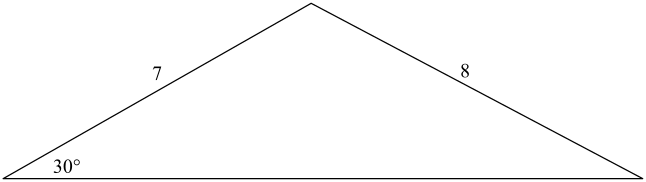
\includegraphics[ width=4.2739in, height=1.2202in,]{L4SZ281Z}
}


Because $8 >7$ this is the one solution case. 

1. Find $B$
\begin{align*}\frac{\sin  B}{b} &  = \frac{\sin  A}{a} \\
\sin  B &  = \frac{b \sin  A}{a} \\
 &  = \frac{7 \sin  30 \mbox{{\ensuremath{{}^\circ}}}}{8} =0.4375 \\
B &  = \sin ^{ -1} 0.4375 \approx 25.94 \mbox{{\ensuremath{{}^\circ}}}\end{align*}

2. Find $C$
\begin{align*}C &  = 180 \mbox{{\ensuremath{{}^\circ}}} -(30 \mbox{{\ensuremath{{}^\circ}}} +25.94 \mbox{{\ensuremath{{}^\circ}}}) \\
 &  = 124.06 \mbox{{\ensuremath{{}^\circ}}}\end{align*}

3. Find $c$
\begin{align*}\frac{c}{\sin  C} &  = \frac{a}{\sin  A} \\
c &  = \frac{a \sin  C}{c} \\
 &  = \frac{7 \sin  124.06 \mbox{{\ensuremath{{}^\circ}}}}{\sin  30 \mbox{{\ensuremath{{}^\circ}}}} \\
 &  \approx   11.6\end{align*}

\subsubsection{Example 3}
Given $A =30 \mbox{{\ensuremath{{}^\circ}}}$, $a =6$ and $b =7$ solve the triangle. 

In this case $b \sin  A =3.5$ and $b =7$ so as $a$ lies between $3.5$ and $7$. This is the ambiguous case, therefore there are two solutions. 


%TCIMACRO{\TeXButton{Start Two Columns}{\columnsep =30pt
% \begin {multicols}{2}}}%
%BeginExpansion
\columnsep =30pt
\begin {multicols}{2}
%EndExpansion
 

   
\setlength\fboxrule{0in}\setlength\fboxsep{0.2in}\fcolorbox[HTML]{000000}{FFFFFF}{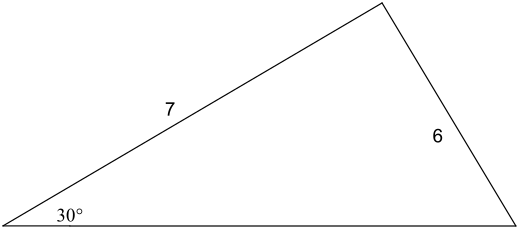
\includegraphics[ width=2.8885in, height=1.2825in,]{L4SZ2820}
}


   
\setlength\fboxrule{0in}\setlength\fboxsep{0.2in}\fcolorbox[HTML]{000000}{FFFFFF}{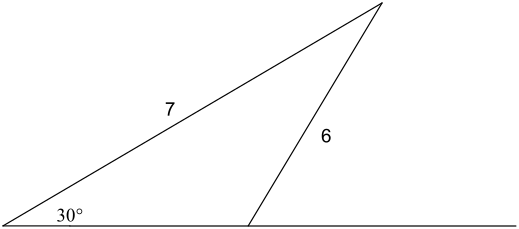
\includegraphics[ width=2.9308in, height=1.3015in,]{L4SZ2821}
}



%TCIMACRO{\TeXButton{End Two Columns}{\end {multicols}}}%
%BeginExpansion
\end {multicols}
%EndExpansion
 

It
is best to visualise these two solutions on the same diagram so that the isosceles triangle can help lead to the two results. 

   
\setlength\fboxrule{0in}\setlength\fboxsep{0.2in}\fcolorbox[HTML]{000000}{FFFFFF}{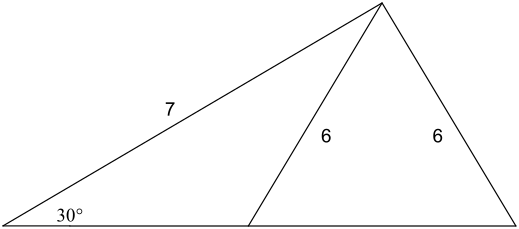
\includegraphics[ width=2.9585in, height=1.3136in,]{L4SZ2822}
}


 \textbf{First solution} (Proceed as before) 

1. Find $B$
\begin{align*}\frac{\sin  B}{b} &  = \frac{\sin  A}{a} \\
\sin  B &  = \frac{b \sin  A}{a} \\
 &  = \frac{7 \sin  30 \mbox{{\ensuremath{{}^\circ}}}}{6} =0.58 \dot{3} \\
B &  = \sin ^{ -1} 0.58 \dot{3} \approx 35.69 \mbox{{\ensuremath{{}^\circ}}}\end{align*}

2. Find $C$
\begin{align*}C &  = 180 \mbox{{\ensuremath{{}^\circ}}} -(30 \mbox{{\ensuremath{{}^\circ}}} +35.69 \mbox{{\ensuremath{{}^\circ}}}) \\
 &  = 114.31 \mbox{{\ensuremath{{}^\circ}}}\end{align*}

3. Find $c$
\begin{align*}\frac{c}{\sin  C} &  = \frac{a}{\sin  A} \\
c &  = \frac{a \sin  C}{\sin  A} \\
 &  = \frac{6 \sin  114.31 \mbox{{\ensuremath{{}^\circ}}}}{\sin  30 \mbox{{\ensuremath{{}^\circ}}}} \\
 &  \approx   10.9\end{align*}

\textbf{Second solution} 

1. Find the second value of $B$ 

\begin{equation*}B =180 \mbox{{\ensuremath{{}^\circ}}} -35.69 \mbox{{\ensuremath{{}^\circ}}} =144.31 \mbox{{\ensuremath{{}^\circ}}}
\end{equation*}

2. Find $C$
\begin{equation*}C =180 \mbox{{\ensuremath{{}^\circ}}} -(30 \mbox{{\ensuremath{{}^\circ}}} +144.31 \mbox{{\ensuremath{{}^\circ}}}) =180 \mbox{{\ensuremath{{}^\circ}}} -174.31 \mbox{{\ensuremath{{}^\circ}}} =5.69 \mbox{{\ensuremath{{}^\circ}}}
\end{equation*}

(Or if you remember the rule that the exterior angle of a triangle is the sum of the two interior
opposite angles $C +30 \mbox{{\ensuremath{{}^\circ}}} =35.69 \mbox{{\ensuremath{{}^\circ}}}$ so $C =35.69 \mbox{{\ensuremath{{}^\circ}}} -30 \mbox{{\ensuremath{{}^\circ}}} =5.69 \mbox{{\ensuremath{{}^\circ}}}$) 

3. Find $c$
\begin{align*}\frac{c}{\sin  C} &  = \frac{a}{\sin  A} \\
c &  = \frac{a \sin  C}{\sin  A} \\
 &  = \frac{6 \sin  5.69 \mbox{{\ensuremath{{}^\circ}}}}{\sin  30 \mbox{{\ensuremath{{}^\circ}}}} \\
 &  \approx   1.2\end{align*}

%\subsection{ }


\subsection{Exercises}

Use the Sine Rule to find side $x$ or angle $\theta $  
%TCIMACRO{\TeXButton{Start Two Columns}{\columnsep =30pt
% \begin {multicols}{2}}}%
%BeginExpansion
\columnsep =30pt
\begin {multicols}{2}
%EndExpansion
 


%TCIMACRO{\TeXButton{End Two Columns}{\end {multicols}}}%
%BeginExpansion
\end {multicols}
%EndExpansion



\begin{description}
\item [1.]   
%TCIMACRO{\TeXButton{Start Two Columns}{\columnsep =30pt
% \begin {multicols}{2}}}%
%BeginExpansion
\columnsep =30pt
\begin {multicols}{2}
%EndExpansion
    
\setlength\fboxrule{0in}\setlength\fboxsep{0.2in}\fcolorbox[HTML]{000000}{FFFFFF}{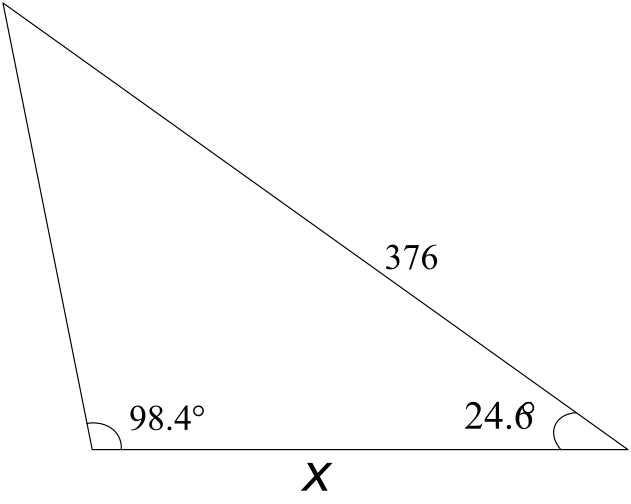
\includegraphics[ width=2.2373in, height=1.7902in,]{L4SZ2823}
}


\item [5]    
\setlength\fboxrule{0in}\setlength\fboxsep{0.2in}\fcolorbox[HTML]{000000}{FFFFFF}{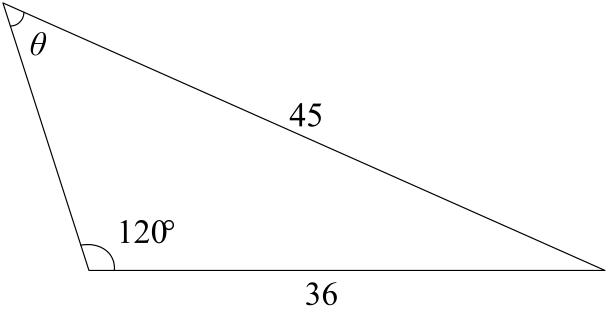
\includegraphics[ width=2.3609in, height=1.241in,]{L4SZ2824}
}
%TCIMACRO{\TeXButton{End Two Columns}{\end {multicols}}}%
%BeginExpansion
\end {multicols}
%EndExpansion
 \end{description}

Solve the triangle using the Sine Rule. 


\begin{description}
\item [7.]    
\setlength\fboxrule{0in}\setlength\fboxsep{0.2in}\fcolorbox[HTML]{000000}{FFFFFF}{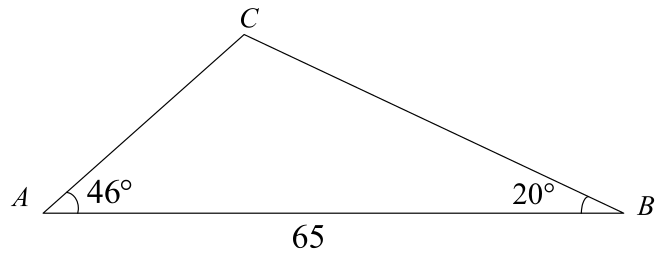
\includegraphics[ width=3.5198in, height=1.3863in,]{L4SZ2825}
}
\end{description}

Sketch each triangle and then solve the triangle using the Sine Rule. 


\begin{description}
\item [9.] $\angle A =50 \mbox{{\ensuremath{{}^\circ}}}\text{,}$ $\angle B =68 \mbox{{\ensuremath{{}^\circ}}}\text{,}$ $c =230$ 

\item [13.] $\angle B =29 \mbox{{\ensuremath{{}^\circ}}}\text{,}$ $\angle C =51 \mbox{{\ensuremath{{}^\circ}}}\text{,}$ $b =44$ 

\item [23.]   
%TCIMACRO{\TeXButton{Start Two Columns}{\columnsep =30pt
% \begin {multicols}{2}}}%
%BeginExpansion
\columnsep =30pt
\begin {multicols}{2}
%EndExpansion
 To find the distance across a river, a surveyor chooses points $A$ and $B$, which are $200 \mbox{ft}$ apart on one side of the river. She then chooses
a reference point $C$ on the opposite side of the river and finds that $\angle BAC \approx 82 \mbox{{\ensuremath{{}^\circ}}}$ and $\angle ABC \approx 52 \mbox{{\ensuremath{{}^\circ}}}\text{.}$  Find the approximate
distance from $A$ to $C$. 

\item    
\setlength\fboxrule{0in}\setlength\fboxsep{0.2in}\fcolorbox[HTML]{000000}{FFFFFF}{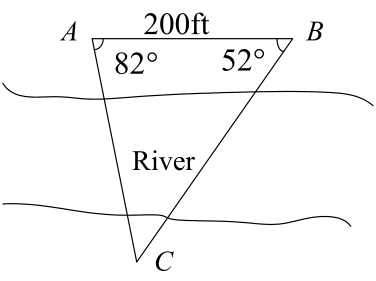
\includegraphics[ width=2.4059in, height=1.7988in,]{L4SZ2826}
}
%TCIMACRO{\TeXButton{End Two Columns}{\end {multicols}}}%
%BeginExpansion
\end {multicols}
%EndExpansion
 

\item [25.]
The path of a satellite circling the earth causes it to pass directly over two tracking stations $A$ and $B$, which are $50 \mbox{mi}$ apart. When the satellite is on one side of the
two stations, the angle of elevation at $A$ and $B$ are measured to be $87.0 \mbox{{\ensuremath{{}^\circ}}}$ and $84.2 \mbox{{\ensuremath{{}^\circ}}}$, respectively. 

\item [(a)]
Draw a diagram. 

\item [(b)] How far is the satellite from
station $A$? 

\item [(c)] How high is the satellite
above the ground? 

\item [27.]   
%TCIMACRO{\TeXButton{Start Two Columns}{\columnsep =30pt
% \begin {multicols}{2}}}%
%BeginExpansion
\columnsep =30pt
\begin {multicols}{2}
%EndExpansion
 A communication tower is located at the top of a steep hill. The angle of inclination
of the hill is $58 \mbox{{\ensuremath{{}^\circ}}}$. A guy wire is attached to the top of the tower
and to the ground, $100 \mbox{m}$ downhill from the base of the tower. The
angle between the slope of the hill and the guy wire is measured as $12 \mbox{{\ensuremath{{}^\circ}}}$. Find $A C$, the length of cable required for the guy wire. 

\item    
\setlength\fboxrule{0in}\setlength\fboxsep{0.2in}\fcolorbox[HTML]{000000}{FFFFFF}{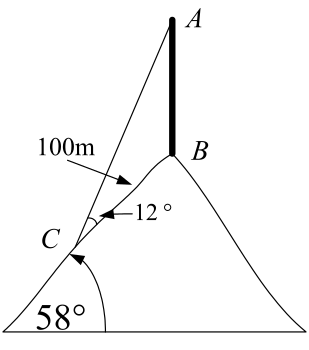
\includegraphics[ width=2.0851in, height=2.3575in,]{L4SZ2827}
}
%TCIMACRO{\TeXButton{End Two Columns}{\end {multicols}}}%
%BeginExpansion
\end {multicols}
%EndExpansion
 

\item [31.]
%TCIMACRO{\TeXButton{Start Two Columns}{\columnsep =30pt
% \begin {multicols}{2}}}%
%BeginExpansion
\columnsep =30pt
\begin {multicols}{2}
%EndExpansion
 A water tower $30 \mbox{m}$ tall is located at the top of a hill. From
a distance of $120 \mbox{m}$ down the hill it is observer that the angle formed between the top and
the base of the tower is $8 \mbox{{\ensuremath{{}^\circ}}}$. Find $\angle ABC\text{,}$ the angle of inclination of the hill. 

\item    
\setlength\fboxrule{0in}\setlength\fboxsep{0.2in}\fcolorbox[HTML]{000000}{FFFFFF}{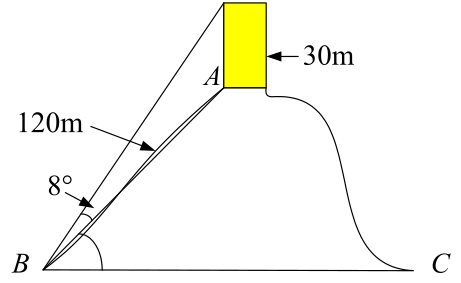
\includegraphics[ width=2.4829in, height=1.5281in,]{L4SZ2828}
}
%TCIMACRO{\TeXButton{End Two Columns}{\end {multicols}}}%
%BeginExpansion
\end {multicols}
%EndExpansion
 \end{description}

%\section{Excel Exercise}
%
%
%\subsection{The Sine Rule - Investigating the Ambiguous Case}
%In the notes we discussed the ambiguous case and we looked at the triangle $ \Delta A B C$. Given $A$, $a$ and $b$ we found two critical values of $a$ that determined whether there would be $0$, $1$ or $2$ solutions for the triangle. The results are summarised in the following table. 
%
%\qquad \qquad \qquad \qquad \qquad
%\begin{tabular}[c]{|c|l|}\hline
%$ <b \sin  A$  & $0$  \\
%\hline
%$ =b \sin  A$  & $1$ solution (right triangle)  \\
%\hline
%$b \sin  A <a <b$  & $2$ solutions  \\
%\hline
%$ =b$  & $1$ solution (one triangle is formed)  \\
%\hline
%$ >b$  & $1$ solution (second triangle invalid)  \\
%\hline
%\end{tabular}
%
%Let $A =30 \mbox{{\ensuremath{{}^\circ}}}$ and let $b =7$ 
%
%The task is to set out in a table the solutions for the triangle for the ambiguous case. (When
%there are 2 solutions.) 
%
%
%\begin{enumerate}
%\item Find the two values of $a$ that define the limits when two solutions are obtained. 
%
%\item Explore Excel
%to check you know how to use the \emph{sine} function. 
%
%\item In a column list values
%of $a$ with increments of $0.1\text{.}$ 
%
%\item Complete the first row of the table to give the two solutions.
%
%
%\item Use \textbf{Fill Down} to complete the table. 
%
%\item Inspect
%the table to ensure you are satisfied you understand the pattern produced. \end{enumerate}
%
%
%Look at the
%values for $c$ and explain why the value at the top of the column is half the value at the bottom. 
%
%Hints: 
%
%
%\begin{enumerate}
%\item Excel requires angles to be measured in radians so convert, (Use $A \times \pi  \div 180$). 
%
%\item To find B use $\sin ^{ -1} \genfrac{(}{)}{}{}{b \sin  A}{a}$. This angle is in radians so must now be converted to degrees. 
%
%\item To
%find $\sin ^{ -1}$ use the function a$\sin \text{.}$ (This is short for $\arcsin $ which is what Excel and some textbooks use for $\sin ^{ -1}\text{.}$) 
%
%\item To find $C$ use $180 -(A +B)$ 
%
%\item To find $c$ convert $A$ and $C$ to radians ($ \times 180 \div \pi $) and use $c =\frac{a \sin  C}{\sin  A}$ \end{enumerate}
%
%
%An example of the final result can be found below. 
%
%   
%\setlength\fboxrule{0.01in}\setlength\fboxsep{0.2in}\fcolorbox[HTML]{000000}{FFFFFF}{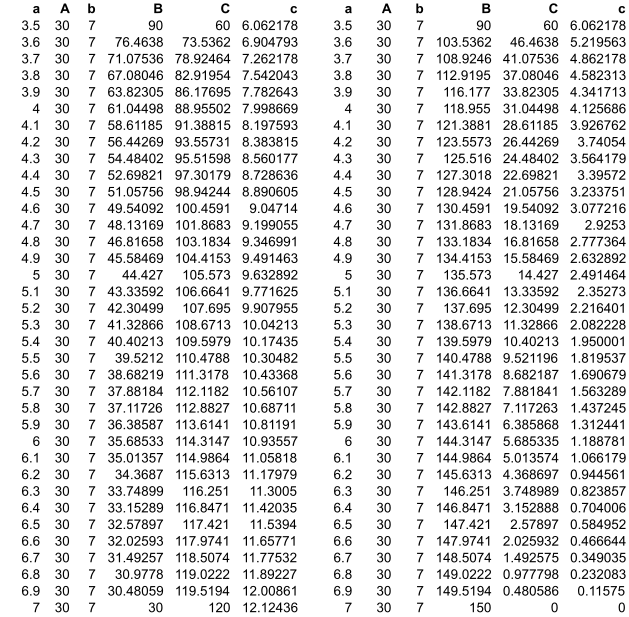
\includegraphics[ width=6.077in, height=5.9698in,]{L4SZ2829}
%}
%
%
%
%%TCIMACRO{\TeXButton{Start Two Columns}{\columnsep =30pt
%% \begin {multicols}{2}}}%
%%BeginExpansion
%\columnsep =30pt
%\begin {multicols}{2}
%%EndExpansion
% 
%
%
%%TCIMACRO{\TeXButton{End Two Columns}{\end {multicols}}}%
%%BeginExpansion
%\end {multicols}
%%EndExpansion
% 

\section{The Cosine Rule}


In this section we will state and prove the Cosine Rule (which is called "The Law of Cosines" in the
textbook). The proof is given here for completeness. You will not
be tested on your ability to reproduce it. The section will give examples where the Cosine Rule is used to solve
problems using the \emph{triangle of vectors} and we will include revision of \emph{bearings} and the use of trigonometry
in \emph{navigation}. 

In this course we have mentioned so far two formulae for the area of a triangle and many problems
allow us to use one of those two formulae. There is a third formula that is used when the three sides of the
triangle are given. In practical situations this is often the easiest and most likely data that has been collected
so this method might be the most useful of the three. The formula is named after the person who first derived
it. It is called \emph{Heron's Formula}. 

\subsection{Proof of The Cosine Rule}
\textbf{To prove:} For any triangle $ \Delta A B C\text{,}$ $a^{2} =b^{2} +c^{2} -2 b c \cos  A$  
%TCIMACRO{\TeXButton{Start Two Columns}{\columnsep =30pt
% \begin {multicols}{2}}}%
%BeginExpansion
\columnsep =30pt
\begin {multicols}{2}
%EndExpansion
 

\vspace{2cm}
\setlength\fboxrule{0in}\setlength\fboxsep{0.2in}\fcolorbox[HTML]{000000}{FFFFFF}{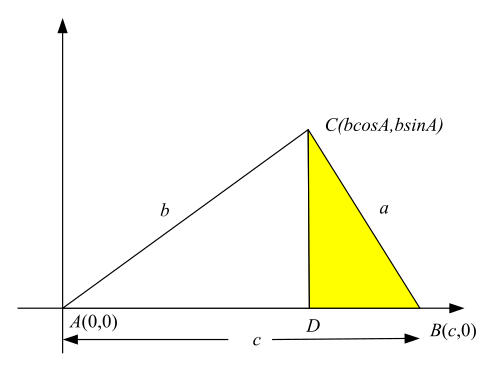
\includegraphics[ width=3.1021in, height=2.3549in,]{L4SZ282A}
}
By Pythagoras Theorem
\begin{align*}B C^{2} &  = C D^{2} +D B^{2} \\
a^{2} &  = \left (c -b \cos  A\right )^{2} +\left (b \sin  A\right )^{2} \\
 &  = c^{2} -2 b c \cos  A +b^{2} \cos ^{2} A +b^{2} \sin ^{2} A \\
 &  = c^{2} -2 b c \cos  A +b^{2} \left (\cos ^{2} A +\sin ^{2} A\right ) \\
 &  = c^{2} -2 b c \cos  A +b^{2}\text{as}\cos ^{2} A +\sin ^{2} A =1\text{\ }\end{align*} 
%TCIMACRO{\TeXButton{End Two Columns}{\end {multicols}}}%
%BeginExpansion
\end {multicols}
%EndExpansion
 

This is usually written
\begin{equation*}a^{2} =b^{2} +c^{2} -2 b c \cos  A
\end{equation*}

The diagram has been drawn to simplify the way the proof unfolds. You
will see that by placing the vertex $A$ at the origin the side $a$ is found in terms of $b$, $c$, and $A$. The proof would have been the same had $A$ and $B$ been as shown and $C$ placed in the second quadrant. (Thus producing a triangle with an obtuse angle at
$A$.) This rule is symmetrical. You need
to be given two sides and the included angle ($b$, $c$ and $A$) and the formula allows you to calculate $a$. Most textbooks will therefore show you three equivalent formulae
\begin{align*}a^{2} &  = b^{2} +c^{2} -2 b c \cos  A \\
b^{2} &  = c^{2} +a^{2} -2 c a \cos  B \\
c^{2} &  = a^{2} +b^{2} -2 a b \cos  C\end{align*}

In this course you will only be given one formula and you will have to know it is a reminder to
lay out your solution in this way. In particular to remind you where to put the plus and minus signs. 

\subsubsection{Example 1}
Given $a =5$, $b =6$ and $C =50 \mbox{{\ensuremath{{}^\circ}}}$, find $c$.
\begin{align*}c^{2} &  = a^{2} +b^{2} -2 a b \cos  C \\
 &  = 5^{2} +6^{2} -2 \times 5 \times 6 \times \cos  50 \mbox{{\ensuremath{{}^\circ}}} \\
 &  \approx   22.43274342 \\
c &  \approx   \sqrt{22.43274342} \\
 &  \approx   4.736321718 \approx 4.7 \left (1\text{dp}\right )\end{align*}

\subsubsection{Example 2}
Given $a =5$, $b =6$ and $C =130 \mbox{{\ensuremath{{}^\circ}}}$, find $c$.
\begin{align*}c^{2} &  = a^{2} +b^{2} -2 a b \cos  C \\
 &  = 5^{2} +6^{2} -2 \times 5 \times 6 \times \cos  130 \mbox{{\ensuremath{{}^\circ}}} \\
 &  \approx   99.56725658 \\
c &  \approx   \sqrt{99.56725658} \\
 &  \approx   9.97833937 \approx 10.0 \left (1\text{dp}\right )\end{align*}

These two examples show that when the two sides and the included angle are given the third side
(opposite the given angle) can be found. This is more useful when a practical example is given and example 1
p 513-514 talks about a surveyor using the Cosine Rule to measure the length of a tunnel. However when the problem
is analysed it is still just what we have covered in example 1 above. 

\subsection{To Find an Angle Given Three Sides}
The Cosine Rule states $a^{2} =b^{2} +c^{2} -2 b c \cos  A\text{.}$ So if $a$, $b$, and $c$ are given $A$ can be calculated. The formula can be rearranged as follows
\begin{align*}2 b c \cos  A &  = b^{2} +c^{2} -a^{2} \\
\cos  A &  = \frac{b^{2} +c^{2} -a^{2}}{2 b c}\end{align*}


\begin{enumerate}
\item Again to use this formula you must appreciate the symmetry and the pattern of the numbers otherwise you are
just blindly substituting in a formula without understanding. Notice the fact that the minus sign is in front
of the $a^{2}$ term and a is opposite the angle we are finding. 

\item Notice the $b$ and $c$ are the sides that include the angle we are finding and these sides appear in both the numerator and denominator. Because
of the symmetry of the result we can write
\begin{align*}\cos  A &  = \frac{b^{2} +c^{2} -a^{2}}{2 b c} \\
\cos  B &  = \frac{c^{2} +a^{2} -b^{2}}{2 c a} \\
\cos  C &  = \frac{a^{2} +b^{2} -c^{2}}{2 a b}\end{align*}\end{enumerate}


In this course you will be given one formula which
you should use by following the pattern it produces. 

\subsubsection{Example 3}
Given $a =5$, $b =6$ and $c =9$, find $A$. 

Because $a$ is the smallest side $A$ will most certainly be an acute angle.
\begin{align*}\cos  A &  = \frac{b^{2} +c^{2} -a^{2}}{2 b c} \\
 &  = \frac{6^{2} +9^{2} -5^{2}}{2 \times 6 \times 9} \\
 &  \approx 0.851851851 \\
A &  \approx \cos ^{ -1} \left (0.851851851\right ) \\
 &  \approx 31.6 \mbox{{\ensuremath{{}^\circ}}}\end{align*}

\subsubsection{Example 4}
For example 3 find $C$.
\begin{align*}\cos  C &  = \frac{a^{2} +b^{2} -c^{2}}{2 a b} \\
 &  = \frac{6^{2} +5^{2} -9^{2}}{2 \times 6 \times 5} \\
 &  \approx  -0. \dot{3} \\
C &  \approx \cos ^{ -1} \left ( -0. \dot{3}\right ) \\
 &  \approx 109.4712206 \\
 &  \approx 109.5 \mbox{{\ensuremath{{}^\circ}}}\end{align*}

\subsection{Navigation}
In a navigation question the direction is often given as a bearing. Thus $N 40 \mbox{{\ensuremath{{}^\circ}}} W$ is said "North $40 \mbox{{\ensuremath{{}^\circ}}}$ West" or "$40 \mbox{{\ensuremath{{}^\circ}}}$ West of North", and means start facing North and rotate $40 \mbox{{\ensuremath{{}^\circ}}}$ in a Westerly direction. A vector in this direction
is represented by an arrow. 

   
\setlength\fboxrule{0in}\setlength\fboxsep{0.2in}\fcolorbox[HTML]{000000}{FFFFFF}{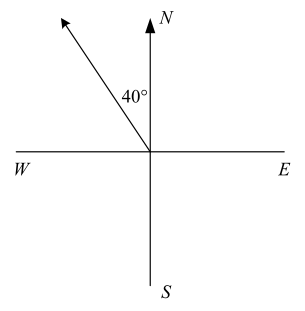
\includegraphics[ width=2.3817in, height=2.4284in,]{L4SZ282B}
}


A journey therefore can comprise a sequence of direction changes and potential speed changes. A
trap in these problems is to confuse distances and speeds. You must read your question carefully and make sure
that every vector on the diagram has been correctly converted so that they are all either distances or speeds. 

\subsubsection{Example}
A fisherman leaves his home port and heads in a direction $N 70 \mbox{{\ensuremath{{}^\circ}}} W$. He travels $48 \mbox{km}$ to reach his first fishing spot. The following
day he travels in a direction $N 10 \mbox{{\ensuremath{{}^\circ}}} E$ at $8 \mbox{km}$/$\mbox{h}$ for $10$ hours to reach his second fishing spot. 


\begin{description}
\item [(a)] How far is he from his home port when he arrives at his second
fishing spot? 

\item [(b)] What is the bearing of the home
port from his second fishing spot? 
\end{description}

The first journey is in $\mbox{km}$ so the second journey must be in $\mbox{km}$ too so that we can draw a triangle of vectors. $8 \mbox{km}$/$\mbox{h}$ for $10$ hours is $80 \mbox{km}$. Assume both journeys are in straight lines. 
\columnsep =30pt
\begin {multicols}{2}

\textbf{Strategy:}
\begin{enumerate}
\item [I] Make a reasonable sized diagram so that the NSEW axes can be placed at each
vertex of the triangle of vectors. 

\item [II] Don't forget about corresponding
angles and alternate angles because the NSEW axes create parallel lines. \end{enumerate}
    
\setlength\fboxrule{0in}\setlength\fboxsep{0.2in}\fcolorbox[HTML]{000000}{FFFFFF}{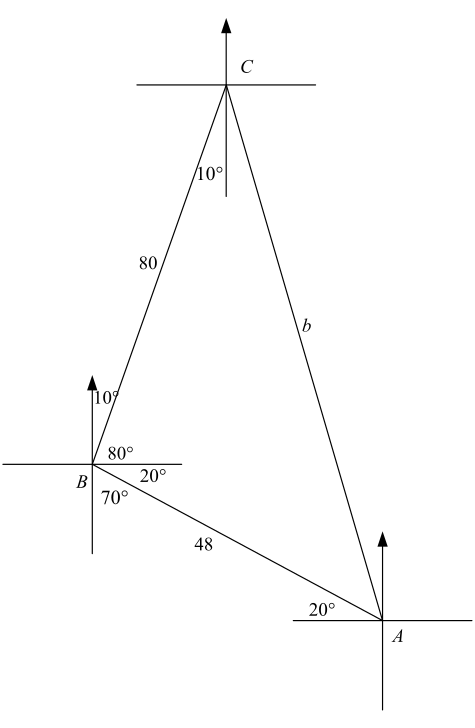
\includegraphics[ width=3.4817in, height=5.3082in,]{L4SZ282C}
}

\begin{enumerate}
\item Sketch the situation. 

\item Use your knowledge of parallel
lines to show the angle (between the two journeys) at $B$ is $100 \mbox{{\ensuremath{{}^\circ}}}$. 

\item (a) You have two sides ($48$ and $80$) and the included angle ($100 \mbox{{\ensuremath{{}^\circ}}}$) so the\ Cosine Rule can be used to find $A C$ the journey back to port.
\begin{align*}b^{2} &  = c^{2} +a^{2} -2 c a \cos  B \\
 &  = 48^{2} +80^{2} -2 \times 48 \times 80 \times \cos  100 \mbox{{\ensuremath{{}^\circ}}} \\
 &  \approx   10037.618 \\
b &  \approx   100.1879135 \approx 100 \mbox{km}\end{align*}

\item (b) To find the bearing you must first find another angle
in the triangle. Find $C$. (Use the Sine Rule or Cosine Rule - both should work.)
\begin{align*}\frac{\sin  C}{c} &  = \frac{\sin  B}{b} \\
\sin  C &  = \frac{c \sin  B}{b} \\
 &  \approx   \frac{48 \sin  100 \mbox{{\ensuremath{{}^\circ}}}}{100} \\
 &  \approx   0.472707721 \\
C &  \approx   \sin ^{ -1} 0.472707721 \\
 &  \approx   28.21020463 \mbox{{\ensuremath{{}^\circ}}} \approx 28 \mbox{{\ensuremath{{}^\circ}}}\end{align*}\end{enumerate}



%TCIMACRO{\TeXButton{End Two Columns}{\end {multicols}}}%
%BeginExpansion
\end {multicols}
%EndExpansion


Put the $28 \mbox{{\ensuremath{{}^\circ}}}$ on the diagram and show that the angle between the vertical and the journey back to port
is $18 \mbox{{\ensuremath{{}^\circ}}}$. Bearing from South is $S 18 \mbox{{\ensuremath{{}^\circ}}} E\text{.}$ Bearing from North is $N 162 \mbox{{\ensuremath{{}^\circ}}} E$ 

\subsection{The Area of Triangle using Heron's Formula}
In this section we show you Heron's Formula to find the area of a triangle given the three sides. We
will then have three formulae that you could use and each requires different facts to be given. 


\begin{tabular}[c]{|l|l|}\hline
\textbf{Given}
& \textbf{Area}  \\
\hline
Base and height
& $\frac{1}{2} \times $ base $ \times $ height  \\
\hline
2 sides and the included angle
($a$,$b$ and $C$)  & $\frac{1}{2} a b \sin  C$  \\
\hline
3 sides ($a$, $b$ and $c$)  & $\sqrt{s \left (s -a\right ) \left (s -b\right ) \left (s -c\right )}$ where $s =\frac{1}{2} \left (a +b +c\right )$  \\
\hline
\end{tabular}

$s$ is called the \emph{semiperimeter}. 

We will not discuss this proof in this course. Heron's
formula is very useful because you are more likely in practice to be required to find the area of a triangle whose sides are given than being given the
base and height or two sides and the included angle. 

\subsubsection{Example}
Given a triangle whose sides are $9 \mbox{cm}$, $10 \mbox{cm}$, and $11 \mbox{cm}$, find its area.
\begin{align*}s &  = \frac{1}{2} \left (9 +10 +11\right ) \\
 &  = 15 \\
\text{Area} &  = \sqrt{15 (15 -9) (15 -10) (15 -11)} \\
 &  = \sqrt{15 \times 6 \times 5 \times 4} \\
 &  \approx 42.42640687 \approx 42 cm^{2}\end{align*}

\subsection{Exercises}
The following exercises from pp 518-521 have been covered in this section: 


\begin{description}
\item [1.]   
%TCIMACRO{\TeXButton{Start Two Columns}{\columnsep =30pt
% \begin {multicols}{2}}}%
%BeginExpansion
\columnsep =30pt
\begin {multicols}{2}
%EndExpansion
 Use the Cosine Rule to find $x$ 

\item    
\setlength\fboxrule{0in}\setlength\fboxsep{0.2in}\fcolorbox[HTML]{000000}{FFFFFF}{\includegraphics[ width=2.8236in, height=1.3007in,]{L4SZ282D}
}
\vspace*{1.5cm} 

\item [5.]
Use the Cosine Rule to find $\theta $ 

\item    
\setlength\fboxrule{0in}\setlength\fboxsep{0.2in}\fcolorbox[HTML]{000000}{FFFFFF}{\includegraphics[ width=1.2747in, height=1.7262in,]{L4SZ282E}
}
%TCIMACRO{\TeXButton{End Two Columns}{\end {multicols}}}%
%BeginExpansion
\end {multicols}
%EndExpansion
 \end{description}

Solve the triangle ABC for questions 9, 13, and 15. 


\begin{description}
\item [9.]    
\setlength\fboxrule{0in}\setlength\fboxsep{0.2in}\fcolorbox[HTML]{000000}{FFFFFF}{\includegraphics[ width=2.693in, height=0.9798in,]{L4SZ282F}
}


\item [13.] $a =20\text{,}$ $b =25\text{,}$ $c =22$ 

\item [15.] $b =125\text{,}$ $c =162\text{,}$ $\angle B =40 \mbox{{\ensuremath{{}^\circ}}}$ \end{description}

For questions 19 and 23 use either the Sine Rule or Cosine
Rule as appropriate. 


\begin{description}
\item [19.]   
%TCIMACRO{\TeXButton{Start Two Columns}{\columnsep =30pt
% \begin {multicols}{2}}}%
%BeginExpansion
\columnsep =30pt
\begin {multicols}{2}
%EndExpansion
    
\setlength\fboxrule{0in}\setlength\fboxsep{0.2in}\fcolorbox[HTML]{000000}{FFFFFF}{\includegraphics[ width=2.5166in, height=1.1234in,]{L4SZ282G}
}


\item [23.]    
\setlength\fboxrule{0in}\setlength\fboxsep{0.2in}\fcolorbox[HTML]{000000}{FFFFFF}{\includegraphics[ width=2.412in, height=1.3309in,]{L4SZ282H}
}
%TCIMACRO{\TeXButton{End Two Columns}{\end {multicols}}}%
%BeginExpansion
\end {multicols}
%EndExpansion
 

\item [27.]
%TCIMACRO{\TeXButton{Start Two Columns}{\columnsep =30pt
% \begin {multicols}{2}}}%
%BeginExpansion
\columnsep =30pt
\begin {multicols}{2}
%EndExpansion
 To find the distance across a small lake, a surveyor has taken the measurements shown. Find
the distance across the lake using this information. 

\item    
\setlength\fboxrule{0in}\setlength\fboxsep{0.2in}\fcolorbox[HTML]{000000}{FFFFFF}{\includegraphics[ width=2.7665in, height=1.5965in,]{L4SZ282I}
}
%TCIMACRO{\TeXButton{End Two Columns}{\end {multicols}}}%
%BeginExpansion
\end {multicols}
%EndExpansion
 

\item [29.]
Two straight roads diverge at an angle of $65 \mbox{{\ensuremath{{}^\circ}}}$. Two cars leave the intersection at $2.00$ P.M., one traveling at $50 mi/\mbox{h}$ and the other at $30 mi/\mbox{h}$. How far apart are the cars at $2.30$ P.M.? 

\item [31.] A pilot flies
in a straight path for $1 \mbox{h}\; 30 \mbox{min}$. She then makes a course correction, heading $10 \mbox{{\ensuremath{{}^\circ}}}$ to the right of her original course, and flies for $2 \mbox{h}$ in the new direction. If she
maintains a constant speed of $625 mi/\mbox{h}$ how far is she from her starting point? 

\item [33.]
A fisherman leaves his home port and heads in a direction N $70 \mbox{{\ensuremath{{}^\circ}}}$ W. he travels $30 \mbox{mi}$ and reaches Egg Island. The next day he sails N
$10 \mbox{{\ensuremath{{}^\circ}}}$ E for $50 \mbox{mi}$, reaching Forrest Island. 

\item [(a)]
Find the distance between the fisherman's home port and Forrest Island. 

\item [(b)]
Find the bearing from Forrest Island back to his home port. 

\item [35.]
A triangular field has sides of lengths $22$, $36$, and $44$ yd. Find the largest angle. 

\item [37.]
A boy is flying two kites at the same time. He has $380 \mbox{ft}$ of line out to one kite and $420 \mbox{ft}$ of line out to the other. He estimates the angle
between the two lines is $30 \mbox{{\ensuremath{{}^\circ}}}$. Find the approximate distance between the two
kites. 

\item [39.]   
%TCIMACRO{\TeXButton{Start Two Columns}{\columnsep =30pt
% \begin {multicols}{2}}}%
%BeginExpansion
\columnsep =30pt
\begin {multicols}{2}
%EndExpansion
 A steep mountain is inclined $74 \mbox{{\ensuremath{{}^\circ}}}$ to the horizontal and rises $3400 \mbox{ft}$ above the surrounding plain. A cable car is to
be installed from a point $800 \mbox{ft}$ from the base to the top of the mountain, as shown. Find
the shortest length of cable needed. 

\item    
\setlength\fboxrule{0in}\setlength\fboxsep{0.2in}\fcolorbox[HTML]{000000}{FFFFFF}{\includegraphics[ width=2.4587in, height=1.5912in,]{L4SZ282J}
}
%TCIMACRO{\TeXButton{End Two Columns}{\end {multicols}}}%
%BeginExpansion
\end {multicols}
%EndExpansion
 \end{description}


\begin{description}
\item [41.] Three circles of radii $4$, $5$, and $6 \mbox{cm}$ respectively are mutually tangent. Find the area
enclosed between the circles. 

\item \qquad \qquad \qquad \qquad
\setlength\fboxrule{0in}\setlength\fboxsep{0.2in}\fcolorbox[HTML]{000000}{FFFFFF}{\includegraphics[ width=3.3269in, height=2.6394in,]{L4SZ282K}
}


\item [43.]   
%TCIMACRO{\TeXButton{Start Two Columns}{\columnsep =30pt
% \begin {multicols}{2}}}%
%BeginExpansion
\columnsep =30pt
\begin {multicols}{2}
%EndExpansion
 A surveyor wishes to find the distance between two points $A$ and $B$ on the opposite side of a river. on her side of the river she chooses two points
$C$ and $D$ that are $20 \mbox{m}$ apart and measures the angles shown. Find
the distance between $A$ and $B\text{.}$ 

\item    
\setlength\fboxrule{0in}\setlength\fboxsep{0.2in}\fcolorbox[HTML]{000000}{FFFFFF}{\includegraphics[ width=2.5028in, height=1.9995in,]{L4SZ282L}
}
%TCIMACRO{\TeXButton{End Two Columns}{\end {multicols}}}%
%BeginExpansion
\end {multicols}
%EndExpansion
 

\item [45.]
Land in downtown Columbia is valued at $ \$20$ a square foot. What is the value of a triangular lot with sides of lengths $112$, $148$, and $190 \mbox{ft}$? \end{description}


%TCIMACRO{\TeXButton{Start Two Columns}{\columnsep =30pt
% \begin {multicols}{2}}}%
%BeginExpansion
\columnsep =30pt
\begin {multicols}{2}
%EndExpansion
 


%TCIMACRO{\TeXButton{End Two Columns}{\end {multicols}}}%
%BeginExpansion
\end {multicols}
%EndExpansion
 

\section{Answers}
%TCIMACRO{\TeXButton{Start Two Columns}{\columnsep =30pt
% \begin {multicols}{2}}}%
%BeginExpansion
\columnsep =30pt
\begin {multicols}{2}
%EndExpansion
 

\textbf{Exercises 3.1} 

1. $\frac{\pi }{5} \approx 0.628 \mbox{rad}$ 

3. $\frac{ -8 \pi }{3} \approx  -8.378 \mbox{rad}$ 

5. $\frac{\pi }{3} \approx 1.047 \mbox{rad}$ 

7. $\frac{ -3 \pi }{4} \approx  -2.356 \mbox{rad}$ 

9. $135 \mbox{{\ensuremath{{}^\circ}}}$ 

11. $150 \mbox{{\ensuremath{{}^\circ}}}$ 

13. $\frac{ -270}{\pi } \approx  -85.9 \mbox{{\ensuremath{{}^\circ}}}$ 

15. $ -15 \mbox{{\ensuremath{{}^\circ}}}$ 

41. $\frac{55 \pi }{9} \approx 19.2$ 

43. $4$ 

45. $4 \mbox{mi}$ 

47. $2 \mbox{rad} \approx 114.6 \mbox{{\ensuremath{{}^\circ}}}$ 

49. $\frac{36}{\pi } \approx 11.459 \mbox{m}$ 

51. $330 \pi  \approx 1037 \mbox{mi}$ 

53. $1.6$ million $\mbox{mi}$ 

55. $1.15 \mbox{mi}$ 

57. $50 \mathrm{m}^{2}$ 

59. $4 \mbox{m}$ 

61. $6 cm^{2}$ 

63. $\frac{32 \pi }{15} ft/\mbox{s}$ 

65.(a) $2000 \pi  rad/\mbox{min}$ (b) $\frac{50 \pi }{3} ft/\mbox{s} \approx 52.4 ft/\mbox{s}$ 

67. $39.3 mi/\mbox{h}$ 

69. $2.1 \mathrm{m}/\mbox{s}$ 

\textbf{Exercises 3.2} 

1. $\sin  \theta  =\frac{4}{5} ,\cos  \theta  =\frac{3}{5} ,\tan  \theta  =\frac{4}{3}$ 

3. $\sin  \theta  =\frac{40}{41} ,\cos  \theta  =\frac{9}{41} ,\tan  \theta  =\frac{40}{9}$ 

5. $\sin  \theta  =\frac{2 \sqrt{13}}{13} ,\cos  \theta  =\frac{3 \sqrt{13}}{13} ,\tan  \theta  =\frac{2}{3}$ 

10. $12 \sqrt{2}$ 

11. $\frac{13 \sqrt{3}}{2}$ 

13. $16.51658$ 

29. $45 \mbox{{\ensuremath{{}^\circ}}} ,16 ,16 \sqrt{2} \approx 22.63$ 

31. $38 \mbox{{\ensuremath{{}^\circ}}} ,44.79 ,56.85$ 

35. $1026 \mbox{ft}$ 

37.(a) $2100 \mbox{mi}$ (b) No 

39. $19 \mbox{ft}$ 

42. $600 \sin  65 \mbox{{\ensuremath{{}^\circ}}} \approx 544 \mbox{ft}$ 

43. $345 \mbox{ft}$ 

45. $415 \mbox{ft} ,152 \mbox{ft}$ 

46.$11,379 \mbox{ft}$ 

49. $5808 \mbox{ft}$ 

\textbf{Exercises 3.3} 

7. $\frac{1}{2}$ 

9. $ -\frac{\sqrt{2}}{2}$ 

11. $ -\sqrt{3}$ 

15. $ -\frac{\sqrt{3}}{2}$ 

17. $\frac{\sqrt{3}}{3}$ 

19. $\frac{\sqrt{3}}{2}$ 

21. $ -1$ 

23. $\frac{1}{2}$ 

29. undefined 

41. $\cos  \theta  = -\frac{4}{5} ,\tan  \theta  = -\frac{3}{4}$ 

43. $\sin  \theta  = -\frac{3}{5} ,\cos  \theta  =\frac{4}{5}$ 

49. (a) $\frac{\sqrt{3}}{2} ,\sqrt{3}$ (b) $\frac{1}{2} ,\frac{\sqrt{3}}{4}$ (c) $\frac{3}{4} ,0.88967$ 

51. $19.1$ 

53. $66.1 \mbox{{\ensuremath{{}^\circ}}}$ 

\textbf{Exercises 3.4} 

1. $318.8$ 

5. $44 \mbox{{\ensuremath{{}^\circ}}}$ 

7. $\angle C =114 \mbox{{\ensuremath{{}^\circ}}} ,a \approx 51 ,b \approx 24$ 

9. $\angle C =62 \mbox{{\ensuremath{{}^\circ}}} ,a \approx 200 b \approx 242$ 
%TCIMACRO{\TeXButton{End Two Columns}{\end {multicols}}}%
%BeginExpansion

%EndExpansion
  

13. $\angle A =100 \mbox{{\ensuremath{{}^\circ}}} ,a \approx 89 ,c \approx 71$ 

15. $\angle B \approx 30 \mbox{{\ensuremath{{}^\circ}}} ,\angle C \approx 40 \mbox{{\ensuremath{{}^\circ}}} ,c \approx 19$ 

17. no solution 

19. $\angle A_{1} \approx 125 \mbox{{\ensuremath{{}^\circ}}} ,\angle C_{1} \approx 30 \mbox{{\ensuremath{{}^\circ}}} ,a_{1} \approx 49\text{,}$ 

\  \ $\angle A_{2} \approx 5 \mbox{{\ensuremath{{}^\circ}}} ,\angle C_{2} \approx 150 \mbox{{\ensuremath{{}^\circ}}} ,a_{2} \approx 5.6$ 

23. $219 \mbox{ft}$ 

25. (b) $1018 \mbox{mi}\text{,}$ (c) $1017 \mbox{mi}$ 

27. $155 \mbox{m}$ 

31. $48.2 \mbox{{\ensuremath{{}^\circ}}}$ 

\textbf{Exercises 3.5} 

1. $28.9$ 

5. $29.89 \mbox{{\ensuremath{{}^\circ}}}$ 

9. $\angle A \approx 39.4 \mbox{{\ensuremath{{}^\circ}}} ,\angle B \approx 20.6 \mbox{{\ensuremath{{}^\circ}}} ,c \approx 24.6$ 

13. $\angle A \approx 50 \mbox{{\ensuremath{{}^\circ}}} ,\angle B \approx 73 \mbox{{\ensuremath{{}^\circ}}} ,\angle C \approx 57 \mbox{{\ensuremath{{}^\circ}}}$ 

15. $\angle A_{1} \approx 83.6 \mbox{{\ensuremath{{}^\circ}}} ,\angle C_{1} \approx 56.4 \mbox{{\ensuremath{{}^\circ}}} ,a_{1} \approx 193$ 

\  \ $\angle A_{2} \approx 16.4 \mbox{{\ensuremath{{}^\circ}}} ,\angle C_{2} \approx 123.6 \mbox{{\ensuremath{{}^\circ}}} ,a_{2} \approx 54.9$ 

19. $2$ 

23. $84.6 \mbox{{\ensuremath{{}^\circ}}}$ 

27. $2.30 \mbox{mi}$ 

29. $23.1 \mbox{mi}$ 

31 $2179 \mbox{mi}$ 

33. (a) $62.6 \mbox{mi}$ (b) $S 18.2 \mbox{{\ensuremath{{}^\circ}}} E$ 

35. $96 \mbox{{\ensuremath{{}^\circ}}}$ 

37. $211 \mbox{ft}$ 

39. $3835 \mbox{ft}$ 

41. $3.85 cm^{2}$ 

43. $14.3 \mbox{m}$ 

45. $ \$165,554$ 

\end {multicols}

\section{Trigonometric Functions of Real Numbers}
In this next part of the chapter the three main trigonometric functions (sine, cosine and tangent) will be studied. They
will be viewed as functions of real numbers. This means that the domains of the functions are the real numbers.
The first half viewed the functions in terms of angles. This
means that the domains of the functions will be angles. The trigonometric functions defined in these two ways
are identical and there is a simple rule connecting the domains. Why do we show you the two approaches? Trigonometry
will be used to solve a variety of problems and these can be divided into two groups, dynamic problems and static problems. When
dynamic problems (such as problems involving motion) are being solved real numbers will be used. When
static problems (such as finding distances and angles for triangles) are being solved angles will be used. 

\section{The Unit Circle}
In this session frequent reference will be made to the measurement of distances around the perimeter
of the unit circle. The unit circle is defined as a circle centre $\left (0 ,0\right )$ radius $1$. Its equation is $x^{2} +y^{2} =1$. In mathematics we are always on the lookout for patterns that make our calculations
easier. for instance, recently we discussed the circle $x^{2} +y^{2} =25$. (Circle centre $\left (0 ,0\right )$ radius $5$.) We found the point $\left (3 ,4\right )$ was on the circle ($3^{2} +4^{2} =5^{2}$). The unit circle also has some patterns that you should become familiar with. 

\subsubsection{Example}
Show $\left (\frac{\sqrt{2}}{2} ,\frac{\sqrt{2}}{2}\right )$ is on the unit circle. 

Because we are given
the coordinates of the point we are required to show that $x^{2} +y^{2} =1$. 

$x^{2} +y^{2} =\genfrac{(}{)}{}{}{\sqrt{2}}{2}^{2} +\genfrac{(}{)}{}{}{\sqrt{2}}{2}^{2} =\frac{2}{4} +\frac{2}{4} =\frac{1}{2} +\frac{1}{2} =1$ 

So $x^{2} +y^{2} =1$ proves that $\left (\frac{\sqrt{2}}{2} ,\frac{\sqrt{2}}{2}\right )$ lies on the unit circle. 

\subsubsection{Example}
Given $\left (\frac{1}{2} ,a\right )$ lies on the unit circle find $a$. 

Because we are told the point lies on the unit circle we substitute
\begin{align*}\genfrac{(}{)}{}{}{1}{2}^{2} +a^{2} &  = 1 \\
	\frac{1}{4} +a^{2} &  = 1 \\
	a^{2} &  = 1 -\frac{1}{4} =\frac{3}{4} \\
	a &  =  \pm \sqrt{\frac{3}{4}} = \pm \frac{\sqrt{3}}{\sqrt{4}} = \pm \frac{\sqrt{3}}{2}\end{align*}

This means there are two possible solutions $\left (\frac{1}{2} ,\frac{\sqrt{3}}{2}\right )$ and $\left (\frac{1}{2} , -\frac{\sqrt{3}}{2}\right )$. A diagram will show
this to you. Notice the right angled triangle we can draw to produce the result. 


\subsection{Terminal Points}
An important skill we require in this section is to be able to connect the coordinates of a point on the unit circle with a length on the circumference
of the unit circle. For this we have a convention. \emph{All
	distances are measured anticlockwise from the point }$\left (1 ,0\right )$. (Books may use
the word counterclockwise in place of anticlockwise. These words are used interchangeably.) In
the digital world of today these terms are not as widely used as they were when only analog clocks had been invented. We
find them convenient words to use because they explain precisely what we want to say. 

We let $t$ be the distance to a point on the unit circle from the point $\left (1 ,0\right )$. $t$ is a real number so distances that are measured in an anticlockwise direction are positive and distances measured in a clockwise
direction are negative. 

\textbf{Definition:} When you measure a distance of $t$ around the perimeter of the unit circle and arrive at a point $P (x ,y)$ the point $P (x ,y)$ is defined as a \emph{terminal point}.

Some terminal points are easy to find provided you remember how to find the perimeter of the unit circle.
\begin{align*}\text{Perimeter} &  = 2 \pi  r\text{\  but if}r =1 \\
	&  = 2 \pi  \times 1 =2 \pi \end{align*}

This means that if you measure from $\left (1 ,0\right )$ right around the unit circle to the starting point $t =2 \pi $. So if $t =2 \pi $ the terminal point is $\left (1 ,0\right )$. 

\subsubsection{Example}
Find the coordinates of the terminal point when (a) $t =\pi $ (b) $t =5 \pi $ (c) $t =\frac{ -3 \pi }{2}$ 

Terminal points are obtained from a sketch of the situation. 

(a) $\left ( -1 ,0\right )$ (b) $\left ( -1 ,0\right )$ (c) $\left (0 ,1\right )$ 

There are other values we will use
that are more easily deduced once chapter 6 in the textbook has been completed. At this stage it is easier to
state these in a table and focus on using the values obtained to solve other related problems. 

We give the terminal point for $0$, $\frac{\pi }{6}$, $\frac{\pi }{4}$, $\frac{\pi }{3}$ and $\frac{\pi }{2}$. 


\begin{tabular}[c]{|r|l|l|l|l|l|}\hline
	$t$  & $0$  & $\frac{\pi }{6}$  & $\frac{\pi }{4}$  & $\frac{\pi }{3}$  & $\frac{\pi }{2}$  \\
	\hline
	Terminal Point  & $\left (1 ,0\right )$  & $\left (\frac{\sqrt{3}}{2} ,\frac{1}{2}\right )$  & $\left (\frac{\sqrt{2}}{2} ,\frac{\sqrt{2}}{2}\right )$  & $\left (\frac{1}{2} ,\frac{\sqrt{3}}{2}\right )$  & $\left (0 ,1\right )$  \\
	\hline
\end{tabular}

These will be given if required in a test. 

\subsubsection{Example}
Use the table to find the terminal points for (a) $t =\frac{5 \pi }{3}$ (b) $t =\frac{ -7 \pi }{6}$ 

(a) $\left (\frac{1}{2} ,\frac{ -\sqrt{3}}{2}\right )$ (b) $\left (\frac{ -\sqrt{3}}{2} ,\frac{1}{2}\right )$ 

Examples 3 and 4 pp 411-413 are about finding
terminal points. 

\subsection{Reference Numbers}
A useful way to connect the terminal point with the distance around the unit circle $t$ is to define a further quantity, the \emph{reference number} $\bar{t}$. However if you understand how to relate a particular value of $t$ with an appropriate value in the first quadrant to allow you to use the table then the need for the definition of a reference
number may be unnecessary. In this course we will tackle problems using the approach given in example 4 above
until the need to define the reference number is unavoidable. 

\subsection{Exercises}
Show that the point is on the unit circle. 


\begin{description}
	\item [1.]   
	%TCIMACRO{\TeXButton{Start Two Columns}{\columnsep =30pt
	% \begin {multicols}{2}}}%
	%BeginExpansion
	\columnsep =30pt
	\begin {multicols}{2}
	%EndExpansion
	$\left (\frac{3}{5} ,\frac{4}{5}\right )$ 
	
	\item [3.]
	$\left ( -\frac{2}{3} , -\frac{\sqrt{5}}{3}\right )$ 
	%TCIMACRO{\TeXButton{End Two Columns}{\end {multicols}}}%
	%BeginExpansion
	\end {multicols}
	%EndExpansion
\end{description}

The point $P$ is on the unit circle. Find $P (x ,y)$ from the given information. 


\begin{description}
	\item [5.] The $x$-coordinate of $P$ is $\frac{4}{5}$ and $P$ is in quadrant I. 
	
	\item [7.] The
	$y$-coordinate of of $P$ is $\frac{2}{3}$ and the $x$-coordinate is negative. 
	
	\item [9.]
	The $x$-coordinate of $P$ is $ -\sqrt{2}/3$ and $P$ is in quadrant III. \end{description}

Find the terminal point $P (x ,y)$ on the unit circle determined by the given value of $t$. 


\begin{description}
	\item [13.]   
	%TCIMACRO{\TeXButton{Start Two Columns}{\columnsep =30pt
	% \begin {multicols}{2}}}%
	%BeginExpansion
	\columnsep =30pt
	\begin {multicols}{2}
	%EndExpansion
	$t =\frac{\pi }{2}$ 
	
	\item [15.] $t =\frac{5 \pi }{6}$ 
	%TCIMACRO{\TeXButton{End Two Columns}{\end {multicols}}}%
	%BeginExpansion
	\end {multicols}
	%EndExpansion
	
	
	\item [17.]
	%TCIMACRO{\TeXButton{Start Two Columns}{\columnsep =30pt
	% \begin {multicols}{2}}}%
	%BeginExpansion
	\columnsep =30pt
	\begin {multicols}{2}
	%EndExpansion
	$t = -\frac{\pi }{3}$ 
	
	\item [19.] $t =\frac{2 \pi }{3}$ 
	%TCIMACRO{\TeXButton{End Two Columns}{\end {multicols}}}%
	%BeginExpansion
	\end {multicols}
	%EndExpansion
	
	
	\item [21.]
	$t = -\frac{3 \pi }{4}$ 
	
	\item [23.] Suppose that the terminal
	point determined by $t$ is the point $\left (\frac{3}{5} ,\frac{4}{5}\right )$ on the unit circle. Find
	the terminal point determined by each of the following. 
	
	\item [(a)]
	%TCIMACRO{\TeXButton{Start Two Columns}{\columnsep =30pt
	% \begin {multicols}{2}}}%
	%BeginExpansion
	\columnsep =30pt
	\begin {multicols}{2}
	%EndExpansion
	$\pi  -t$ 
	
	\item [(b)] $ -t$ 
	%TCIMACRO{\TeXButton{End Two Columns}{\end {multicols}}}%
	%BeginExpansion
	\end {multicols}
	%EndExpansion
	
	
	\item [(c)]
	%TCIMACRO{\TeXButton{Start Two Columns}{\columnsep =30pt
	% \begin {multicols}{2}}}%
	%BeginExpansion
	\columnsep =30pt
	\begin {multicols}{2}
	%EndExpansion
	$\pi  +t$ 
	
	\item [(d)] $t -\pi $ 
	%TCIMACRO{\TeXButton{End Two Columns}{\end {multicols}}}%
	%BeginExpansion
	\end {multicols}
	%EndExpansion
\end{description}


%TCIMACRO{\TeXButton{Start Two Columns}{\columnsep =30pt
% \begin {multicols}{2}}}%
%BeginExpansion
\columnsep =30pt
\begin {multicols}{2}
%EndExpansion



%TCIMACRO{\TeXButton{End Two Columns}{\end {multicols}}}%
%BeginExpansion
\end {multicols}
%EndExpansion

\section{The Trigonometric Functions of Real Numbers}
In this section we define sine, cosine and tangent based on $t$ as defined in section $7.1$. You need to be very careful to decide which quadrant the terminal point is in
so that the signs of the trigonometric functions are correct. 

\textbf{Definitions:} Given a real number $t$. If we move a distance $t$ around the unit circle starting at the point $\left (1 ,0\right )$ and we arrive at a point $P (x ,y)$ then $x =\cos  t$, $y =\sin  t$ and $\frac{y}{x} =\tan  t$ $\left (x \neq 0\right )$. 

A sketch will show the relationship between
$t$, $x$, and $y$. 

A fundamental relationship between sine, cosine and tangent comes from these definitions
\begin{equation*}\tan  t =\frac{\sin  t}{\cos  t}
\end{equation*}

We call this relationship an \emph{identity} because it is true for all values
of $t$. 

There are six trigonometric functions. The other three are
secant, cosecant and cotangent. The are sometimes referred to as the reciprocal functions because: 

Secant is defined by $\sec  t =\frac{1}{\cos  t} =\frac{1}{x}$ 

Cosecant is defined by co$\sec  t =\frac{1}{\sin  t} =\frac{1}{y}$ ($ =$csc $t$) 

Cotangent is defined by $\cot  t =\frac{1}{\tan  t} =\frac{x}{y}$ $\left (y \neq 0\right )$ 

In this course we will focus on sine, cosine
and tangent and only use secant, cosecant and cotangent when it is unavoidable. 

The table in section 7.1 can now be extended to include
sine, cosine and tangent. 

\qquad \qquad
\begin{tabular}[c]{|c|c|c|c|c|}\hline
	$t$  & Terminal Point  & $x =\cos  t$  & $y =\sin  t$  & $\frac{y}{x} =\tan  t$  \\
	\hline
	$0$  & $\left (1 ,0\right )$  & $1$  & $0$  & $\frac{0}{1} =0$  \\
	\hline
	$\frac{\pi }{6}$  & $\left (\frac{\sqrt{3}}{2} ,\frac{1}{2}\right )$  & $\frac{\sqrt{3}}{2}$  & $\frac{1}{2}$  & $\frac{1}{2} \div \frac{\sqrt{3}}{2} =\frac{1}{2} \times \frac{2}{\sqrt{3}} =\frac{1}{\sqrt{3}} =\frac{\sqrt{3}}{3}$  \\
	\hline
	$\frac{\pi }{4}$  & $\left (\frac{\sqrt{2}}{2} ,\frac{\sqrt{2}}{2}\right )$  & $\frac{\sqrt{2}}{2}$  & $\frac{\sqrt{2}}{2}$  & $\frac{\sqrt{2}}{2} \div \frac{\sqrt{2}}{2} =1$  \\
	\hline
	$\frac{\pi }{3}$  & $\left (\frac{1}{2} ,\frac{\sqrt{3}}{2}\right )$  & $\frac{1}{2}$  & $\frac{\sqrt{3}}{2}$  & $\frac{\sqrt{3}}{2} \div \frac{1}{2} =\frac{\sqrt{3}}{2} \times \frac{2}{1} =\sqrt{3}$  \\
	\hline
	$\frac{\pi }{2}$  & $\left (0 ,1\right )$  & $0$  & $1$  & $\frac{1}{0}$ undefined $\left ( =\infty \right )$  \\
	\hline
\end{tabular}

Should you be asked about secant, cosecant or cotangent you should look up the respective reciprocal relationship and calculate it from that.


\subsubsection{Values of Trigonometric Functions}
The value of a trigonometric function consists of two parts the numerical part and the sign. you
must get both parts correct. In the previous section (example 4) you related the values of a terminal point
to another point in the first quadrant. A point on the unit circle could be in any one of the four quadrants.
\ You should develop an intuitive understanding of how this allows you to be sure of the sign of your answer.


\qquad \qquad \qquad \qquad
\begin{tabular}[c]{|c|c|c|c|c|c|}\hline
	Quadrant  & $x$-coordinate  & $y$-coordinate  & $\cos $  & $\sin $  & $\tan $  \\
	\hline
	$1$  & $ +$  & $ +$  & $ +$  & $ +$  & $ +$  \\
	\hline
	$2$  & $ -$  & $ +$  & $ -$  & $ +$  & $ -$  \\
	\hline
	$3$  & $ -$  & $ -$  & $ -$  & $ -$  & $ +$  \\
	\hline
	$4$  & $ +$  & $ -$  & $ +$  & $ -$  & $ -$  \\
	\hline
\end{tabular}

Some people learn this as a mnemonic All sin tan cos. (Meaning all are positive in the first quadrant, only sine is positive in the second quadrant,
only tangent is positive in the third quadrant and only cosine is positive in the fourth quadrant.) Two little
sentences that are sometimes seen to help you to get this right are "\textbf{A}ll \textbf{s}tudents \textbf{t}ake \textbf{c}alculus," and
"\textbf{ACTS} clockwise." This means that as soon as you know which quadrant the terminal point is in you know the sign of the trigonometric function.


These types of problems will be in two categories 


\begin{enumerate}
	\item Problems where $t$ is a multiple of $\frac{\pi }{6}$ or $\frac{\pi }{4}$ 
	
	\item Problems where $t$ is not a multiple of $\frac{\pi }{6}$ or $\frac{\pi }{4}$ 
	
	\item Our special values of $t$, $0$, $\frac{\pi }{6}$, $\frac{\pi }{4}$, $\frac{\pi }{3}$, $\frac{\pi }{2}$ are all multiple of $\frac{\pi }{6}$ or $\frac{\pi }{4}$. They are all in the first quadrant and lead to our being able to relate our problem back
	to these. when you are asked a question where the value of $t$ is a multiple of a special value of $t$ you are being tested on your ability to relate the question to the value for the special value so you should ensure you have
	answered it to show this. (A calculator answer is not appropriate for these questions.) 
	
	\item When
	$t$ is not one of these special values you should use your calculator set in \emph{radians} mode. \end{enumerate}


\subsubsection{Example}
\begin{description}
	\item [(a)] $\tan  \frac{3 \pi }{4} = -1$ 
	
	\item [(b)] $\sin  \genfrac{(}{)}{}{}{ -7 \pi }{3} =\frac{ -\sqrt{3}}{2}$ 
	
	\item [(c)] $\cos  -2.1 = -0.5048$ (4 dp) \end{description}


\subsection{Even and Odd Functions}
Even functions have the $y$-axis as an axis of symmetry. \\\relax Odd functions have point symmetry about
the origin. 

For even functions $f (x) =f ( -x)$ which is the same as saying $f ( -x) =f (x)$. \\\relax For odd functions $f (x) = -f ( -x)$ which is the same as saying $f ( -x) = -f (x)$. 

When we talk about odd and even functions these ideas keep recurring. Sine,
cosine and tangent can be looked at from this perspective too. Regardless of the quadrant for the terminal point
$\sin  t = -\sin  t$ so sine is an odd function. A diagram shows this. Also
$\cos  t =\cos  ( -t)$ so cosine is an even function. The same diagram shows this 

For the
tangent function
\begin{equation*}\tan  ( -t) =\frac{\sin  ( -t)}{\cos  ( -t)} =\frac{ -\sin  t}{\cos  t} = -\tan  t
\end{equation*}

So tangent is also an odd function. 

This subject will be explored further in
the next section. 

\subsection{The Fundamental Pythagorean Identity}
The unit circle has equation $x^{2} +y^{2} =1$ and we define $x =\cos  t$ and $y =\sin  t$ so
\begin{equation*}x^{2} +y^{2} =1 \leadsto \left (\cos  t\right )^{2} +\left (\sin  t\right )^{2} =1
\end{equation*}

This is always written
\begin{equation*}\sin ^{2} t +\cos ^{2} t =1
\end{equation*}

This is an \emph{identity} which means it is true for all values of $t$. 

We will only cover these two identities: $\tan  t =\frac{\sin  t}{\cos  t}$ and $\sin ^{2} t +\cos ^{2} t =1$. 

\subsection{Exercises}
Give the exact value of the trigonometric function
at the given real number 


\begin{tabular}[c]{rllllllrlllll}3.\vspace*{0.25cm}
	& (a)  & $\sin  \left ( -\frac{\pi }{3}\right )$  &  & (b)  & $\cos  \left ( -\frac{\pi }{3}\right )$  &  & 5.  & (a)
	& $\cos  \pi $  &  & (b)  & $\cos  \left ( -\pi \right )$  \\
	7.\vspace*{0.25cm}  & (a)
	& $\sin  \frac{\pi }{2}$  &  & (b)  & $\sin  \frac{3 \pi }{2}$  &  & 9.  & (a)
	& $\cos  \frac{\pi }{2}$  &  & (b)  & $\cos  \frac{5 \pi }{2}$  \\
	13.\vspace*{0.25cm}  & (a)
	& $\cos  \frac{\pi }{3}$  &  & (b)  & $\cos  \left ( -\frac{\pi }{3}\right )$  &  & 15.  & (a)
	& $\tan  \frac{\pi }{6}$  &  & (b)  & $\tan  \left ( -\frac{\pi }{6}\right )$
\end{tabular}

The terminal point $P (x ,y)$ determined bt t is given. Find $\sin  t$, $\cos  t$ and $\tan  t\text{.}$ 


\begin{tabular}[c]{lllllllllll}27.  & $\left (\frac{3}{5} ,\frac{4}{5}\right )$  &  \  \  \  \  \  \  \  &  &  &  &  &  & 29.
	& $\left (\frac{\sqrt{5}}{4} , -\frac{\sqrt{11}}{4}\right )$  & 
\end{tabular}

Find the approximate value of the trigonometric function using the calculator. 

\begin{tabular}[c]{lllllllllll}35.  & $\sin  1$  &  \   & 37.
	& $\sin  1.2$  &  \   & 39.
	& $\tan  0.8$  &  \   & 41.
	& $\cos  4.1$
\end{tabular}



\section{Trigonometric Graphs - Sine and Cosine}

\subsection{Graphs of the Sine and Cosine Functions}
You should be familiar with the fundamental graphs of $y =\sin  t$ and $y =\cos  t$. These graphs are the basis of this section. Desmos
can easily show you the shape of $y =\sin  t$ and $y =\cos  t$ so if you are asked to draw a rough sketch of these curves you should plot a few key points and draw a smooth curve between them. You
will usually be given the required domain however if you are not you would choose to draw these for one complete cycle ($0 -2 \pi $). To sketch $y =\sin  t$ it is enough to select as key points $t =0$, $\frac{\pi }{2}$, $\pi $, $\frac{3 \pi }{2}$, $2 \pi $. 


\begin{tabular}[c]{|l|l|l|l|l|l|}\hline
	$t$  & $0$  & $\frac{\pi }{2}$  & $\pi $  & $\frac{3 \pi }{2}$  & $2 \pi $  \\
	\hline
	$y =\sin  t$  & $0$  & $1$  & $0$  & $ -1$  & $0$  \\
	\hline
\end{tabular}

Similarly to sketch $y =\cos  t$ the same values of $t$ give 


\begin{tabular}[c]{|l|l|l|l|l|l|}\hline
	$t$  & $0$  & $\frac{\pi }{2}$  & $\pi $  & $\frac{3 \pi }{2}$  & $2 \pi $  \\
	\hline
	$y =\cos  t$  & $1$  & $0$  & $ -1$  & $0$  & $1$  \\
	\hline
\end{tabular}

You will be aware that these curves repeat this pattern every $2 \pi $ where $t$ extends in both the positive and negative directions. 

$0 -2 \pi $ represents one complete cycle. Mathematically we say
\begin{align*}\sin  \left (t +2 n \pi \right ) &  = \sin  t\text{\  for any integer}n \\
	\cos  \left (t +2 n \pi \right ) &  = \cos  t\text{\  for any integer}n\end{align*}

Aside: instead of "for any integer $n$" we can write $ \forall n \in \mathbb{Z}$. 

A function that displays this characteristic is described as \emph{periodic} and for $y =\sin  t$ and $y =\cos  t$ the \emph{period} is $2 \pi $. 

You will often be asked to state the period of a trigonometric function so for sine and cosine it
is wise to remember that often the period is $2 \pi $. This means you need only worry about the distinctly different class of examples
of sine and cosine where the period is not $2 \pi $. 

You will sometimes be asked to sketch a graph for a given number of periods or a given number of cycles. These are two different ways of saying the same thing. 

\subsection{The Transformations of Sine and Cosine}
The six transformations we meet in this course are applied to sine and cosine. 

\begin{enumerate}
	\item Vertical shift 
	\item Horizontal shift 
	\item Vertical stretch 
	\item Horizontal stretch 
	\item Reflection in the $x$-axis 
	\item Reflection in the $y$-axis 
\end{enumerate}

We adopt four approaches to tackle these problems 

\begin{enumerate}
	\item Describe the transformation in words. 
	\item Rough sketch based on transformations. 
	\item Rough sketch based on substitution. 
	\item Desmos
	graph. 
\end{enumerate}


\subsubsection{Example}
Sketch $y =\sin  \left (t -\frac{\pi }{2}\right ) +3$ 

1. This may be considered as a sine curve shifted $\frac{\pi }{2}$ to the right and $3$ upwards. 

\textbf{Definition:} A horizontal shift of a sine curve or cosine curve is called a \emph{phase
	shift}. 

2. Transform the 5 point summary 


\begin{tabular}[c]{|l|l|l|l|l|l|}\hline
	$t$  & $0$  & $\frac{\pi }{2}$  & $\pi $  & $\frac{3 \pi }{2}$  & $2 \pi $  \\
	\hline
	$\sin  t$  & $0$  & $1$  & $0$  & $ -1$  & $0$  \\
	\hline
	$\sin  \left (t -\frac{\pi }{2}\right )$  & $ -1$  & $0$  & $1$  & $0$  & $ -1$  \\
	\hline
	$\sin  \left (t -\frac{\pi }{2}\right ) +3$  & $2$  & $3$  & $4$  & $3$  & $2$  \\
	\hline
\end{tabular}

You would sketch this if required 

3. The difference between this approach and the previous one is that the values are calculated
from the 5 values of $t$. Maybe an additional row containing $t -\frac{\pi }{2}$ values will help. 


\begin{tabular}[c]{|l|l|l|l|l|l|}\hline
	$t$  & $0$  & $\frac{\pi }{2}$  & $\pi $  & $\frac{3 \pi }{2}$  & $2 \pi $  \\
	\hline
	$t -\frac{\pi }{2}$  & $ -\frac{\pi }{2}$  & $0$  & $\frac{\pi }{2}$  & $\pi $  & $\frac{3 \pi }{2}$  \\
	\hline
	$\sin  \left (t -\frac{\pi }{2}\right ) +3$  & $2$  & $3$  & $4$  & $3$  & $2$  \\
	\hline
\end{tabular}

You would sketch this if required. 

4. Desmos confirms this 


\setlength\fboxrule{0.01in}\setlength\fboxsep{0.2in}\fcolorbox[HTML]{000000}{FFFFFF}{\includegraphics[ width=4.427in, height=2.3886in,]{L4SZ270G}
}


You would select the most appropriate way to tackle a problem based on the information given and the outcome expected. 

\subsubsection{Example}
Sketch $y =\cos  (x -\frac{\pi }{6})$ 

You could use a table of values however this is $y =\cos  x$ with a horizontal shift of $\frac{\pi }{6}$ to the right. 

Complete the following to show the answer. (This is the graph of $y =\cos  x .)$ 


\setlength\fboxrule{0.01in}\setlength\fboxsep{0.2in}\fcolorbox[HTML]{000000}{FFFFFF}{\includegraphics[ width=4.9095in, height=2.4275in,]{L4SZ270H}
}


\subsubsection{Example}
Sketch $y =2 \cos  t$ 


\begin{tabular}[c]{|l|l|l|l|l|l|}\hline
	$t$  & $0$  & $\frac{\pi }{2}$  & $\pi $  & $\frac{3 \pi }{2}$  & $2 \pi $  \\
	\hline
	$\cos  t$  & $1$  & $0$  & $ -1$  & $0$  & $1$  \\
	\hline
	$2 \cos  t$  & $2$  & $0$  & $ -2$  & $0$  & $2$  \\
	\hline
\end{tabular}

This is a vertical stretch of 2. You could roughly sketch this or use Desmos. 


\setlength\fboxrule{0.01in}\setlength\fboxsep{0.2in}\fcolorbox[HTML]{000000}{FFFFFF}{\includegraphics[ width=3.09in, height=2.0669in,]{L4SZ270I}
}


In general $y =a \sin  x$ represents a vertical stretch of $y =\sin  x$ by $a$. If $a$ is negative the transformation can either be described as a negative stretch or (preferably) as a \emph{stretch}
of $\left \vert a\right \vert $ followed by a \emph{reflection} in the $x$-axis. Recall the reflection of $y =f \left (x\right )$ in the $x$-axis is $y = -f \left (x\right )$. The number $\left \vert a\right \vert $ is called the \emph{amplitude} for both $y =\sin  x$ and $y =\cos  x\text{.}$ 

If $0 <a <1$ the fractional stretch causes the curve to shrink vertically. For instance the curve
$y =\sin  x$ has a maximum value of $1$ and a minimum value of $ -1$. the curve $y =\frac{1}{2} \sin  x$ has a maximum value of $\frac{1}{2}$ and a minimum value of $ -\frac{1}{2}$. 

\subsubsection{Example}
Sketch $y =\cos  ( -t)\text{.}$ 

Recall the reflection of $y =f (x)$in the $y$-axis is $y =f ( -x)$ so you would expect $y =\cos  ( -t)$ to be the reflection of $y =\cos  t$ in the $y$-axis. 


\begin{tabular}[c]{|l|l|l|l|l|l||l|l|l|l|l|l|l}
	$t$  & $0$  & $\frac{\pi }{2}$  & $\pi $  & $\frac{3 \pi }{2}$  & $2 \pi $  &  & $t$  & $0$  & $\frac{\pi }{2}$  & $\pi $  & $\frac{3 \pi }{2}$  & $2 \pi $  \\
	$ -t$  & $0$  & $ -\frac{\pi }{2}$  & $ -\pi $  & $ -\frac{3 \pi }{2}$  & $ -2 \pi $  &  & $\cos  t$  & $1$  & $0$  & $ -1$  & $0$  & $1$  \\
	$\cos  \left ( -t\right )$  & $1$  & $0$  & $ -1$  & $0$  & $1$  &  &  &  &  &  &  &  \\
	\multicolumn{1}{|l}{
	}
\end{tabular}

You can see from the table at the right that this looks exactly the same as
$y =\cos  t$ so $\cos  t$ is an \emph{even} function. When the $y$-axis is an axis of symmetry the function is an \emph{even} function. 


\setlength\fboxrule{0.01in}\setlength\fboxsep{0.2in}\fcolorbox[HTML]{000000}{FFFFFF}{\includegraphics[ width=4.587in, height=2.1689in,]{L4SZ270J}
}


\subsubsection{Example}
Sketch $y =\sin  \frac{1}{2} x$ 


\begin{tabular}[c]{|l|l|l|l|l|l|l|l|l|l|}\hline
	$x$  & $0$  & $\frac{\pi }{2}$  & $\pi $  & $\frac{3 \pi }{2}$  & $2 \pi $  & $\frac{5 \pi }{2}$  & $3 \pi $  & $\frac{7 \pi }{2}$  & $4 \pi $  \\
	\hline
	$\frac{1}{2} x$  & $0$  & $\frac{\pi }{4}$  & $\frac{\pi }{2}$  & $\frac{3 \pi }{4}$  & $\pi $  & $\frac{5 \pi }{4}$  & $\frac{3 \pi }{2}$  & $\frac{7 \pi }{4}$  & $2 \pi $  \\
	\hline
	$\sin  \frac{1}{2} x$  & $0$  &  & $1$  &  & $0$  &  & $ -1$  &  & $0$  \\
	\hline
\end{tabular}

In this case one cycle is achieved only after $x$ has reached $4 \pi $. The period therefore is $4 \pi $. 


\setlength\fboxrule{0.01in}\setlength\fboxsep{0.2in}\fcolorbox[HTML]{000000}{FFFFFF}{\includegraphics[ width=4.0698in, height=1.9372in,]{L4SZ270K}
}


\subsubsection{Example}
Sketch $y =\cos  2 x$ 


\begin{tabular}[c]{|l|l|l|l|l|l|}\hline
	$x$  & $0$  & $\frac{\pi }{2}$  & $\pi $  & $\frac{3 \pi }{2}$  & $2 \pi $  \\
	\hline
	$2 x$  & $0$  & $\pi $  & $2 \pi $  & $3 \pi $  & $4 \pi $  \\
	\hline
	$\cos  2 x$  & $1$  & $ -1$  & $1$  & $ -1$  & $1$  \\
	\hline
\end{tabular}

Maybe this is enough to enable you to sketch the curve. You notice the zeros that you usually get
in the table are missing and the way to include them is to select intermediate $x$ values. 


\begin{tabular}[c]{|l|l|l|l|l|l|}\hline
	$x$  & $0$  & $\frac{\pi }{4}$  & $\frac{\pi }{2}$  & $\frac{3 \pi }{4}$  & $\pi $  \\
	\hline
	$2 x$  & $0$  & $\frac{\pi }{2}$  & $\pi $  & $\frac{3 \pi }{2}$  & $2 \pi $  \\
	\hline
	$\cos  2 x$  & $1$  & $0$  & $ -1$  & $0$  & $1$  \\
	\hline
\end{tabular}


\setlength\fboxrule{0.01in}\setlength\fboxsep{0.2in}\fcolorbox[HTML]{000000}{FFFFFF}{\includegraphics[ width=3.0666in, height=1.9614in,]{L4SZ270L}
}


Notice by sketching from $0$ to $2 \pi $ $2$ cycles are drawn. The period here is $\pi $. There is a pattern emerging. Given
$y =\sin  k x$ or $y =\cos  k x$. The value of $k$ tells you how many cycles in $2 \pi $. If $k =2$ there are $2$ cycles in $2 \pi $ so one cycle takes $\pi $. If $k =\frac{1}{2}$ there is $\frac{1}{2}$ cycle in $2 \pi $ therefore one cycle will take $4 \pi $. Looking at this the other way. The
period is the interval required for one cycle so when $k =2$ the period $ =\pi $ and when $k =\frac{1}{2}$ the period $ =4 \pi \text{.}$ 

In general given $y =\sin  k x$ or $y =\cos  k x$ the period is $\frac{2 \pi }{k}$. 

In a test or exam, questions will be set to test these concepts, however, the topic can be complicated very
easily and in these cases Desmos or other software should be used to sketch the graph. 

\subsection{Exercises}
Graph the functions by hand. 

\begin{description}
	\item [1.]   
	%TCIMACRO{\TeXButton{Start Two Columns}{\columnsep =30pt
	% \begin {multicols}{2}}}%
	%BeginExpansion
	\columnsep =30pt
	\begin {multicols}{2}
	%EndExpansion
	$y =1 +\sin  x$ 
	
	\item [3.] $y =1 -\cos  x$ 
	%TCIMACRO{\TeXButton{End Two Columns}{\end {multicols}}}%
	%BeginExpansion
	\end {multicols}
	%EndExpansion
	
	\columnsep =30pt
	\begin {multicols}{2}
	\item [5.]
	%TCIMACRO{\TeXButton{Start Two Columns}{\columnsep =30pt
	% \begin {multicols}{2}}}%
	%BeginExpansion
	
	%EndExpansion
	$y = -2 \sin  x$ 
	
	\item [7.] $y =4 -2 \cos  x$ 
	%TCIMACRO{\TeXButton{End Two Columns}{\end {multicols}}}%
	%BeginExpansion
	\end {multicols}
	%EndExpansion
	
	
	\item [9.]
	$y =\left \vert \cos  x\right \vert $ \end{description}

Find the amplitude
and period of the function and sketch its graph. 


\begin{description}
	\item [11.]   
	%TCIMACRO{\TeXButton{Start Two Columns}{\columnsep =30pt
	% \begin {multicols}{2}}}%
	%BeginExpansion
	\columnsep =30pt
	\begin {multicols}{2}
	%EndExpansion
	$y =\cos  4 x$ 
	
	\item [13.] $y =3 \sin  3 x$ 
	%TCIMACRO{\TeXButton{End Two Columns}{\end {multicols}}}%
	%BeginExpansion
	\end {multicols}
	%EndExpansion
	
	
	\item [15.]
	%TCIMACRO{\TeXButton{Start Two Columns}{\columnsep =30pt
	% \begin {multicols}{2}}}%
	%BeginExpansion
	\columnsep =30pt
	\begin {multicols}{2}
	%EndExpansion
	$y =10 \sin  \frac{1}{2} x$ 
	
	\item [17.] $y = -\cos  \frac{1}{3} x$ 
	%TCIMACRO{\TeXButton{End Two Columns}{\end {multicols}}}%
	%BeginExpansion
	\end {multicols}
	%EndExpansion
	
	
	\item [19.]
	$y =3 \cos  3 \pi  x$ \end{description}

Find the amplitude, period and phase shift of the function,
and graph one complete period. 


\begin{description}
	\item [21.]   
	%TCIMACRO{\TeXButton{Start Two Columns}{\columnsep =30pt
	% \begin {multicols}{2}}}%
	%BeginExpansion
	\columnsep =30pt
	\begin {multicols}{2}
	%EndExpansion
	$y =\cos  \left (x -\frac{\pi }{2}\right )$ 
	
	\item [23.] $y = -\sin  \left (x -\frac{\pi }{6}\right )$ 
	%TCIMACRO{\TeXButton{End Two Columns}{\end {multicols}}}%
	%BeginExpansion
	\end {multicols}
	%EndExpansion
	
	
	\item [25.]
	%TCIMACRO{\TeXButton{Start Two Columns}{\columnsep =30pt
	% \begin {multicols}{2}}}%
	%BeginExpansion
	\columnsep =30pt
	\begin {multicols}{2}
	%EndExpansion
	$y =5 \cos  \left (3 x -\frac{\pi }{4}\right )$ 
	
	\item [27.] $y =2 \sin  \left (\frac{2}{3} x -\frac{\pi }{6}\right )$ 
	%TCIMACRO{\TeXButton{End Two Columns}{\end {multicols}}}%
	%BeginExpansion
	\end {multicols}
	%EndExpansion
	
	
	\item [29.]
	%TCIMACRO{\TeXButton{Start Two Columns}{\columnsep =30pt
	% \begin {multicols}{2}}}%
	%BeginExpansion
	\columnsep =30pt
	\begin {multicols}{2}
	%EndExpansion
	$y =3 \cos  \pi  \left (x +\frac{1}{2}\right )$ 
	
	\item [31.] $y = -\frac{1}{2} \cos  \left (2 x -\frac{\pi }{3}\right )$ 
	%TCIMACRO{\TeXButton{End Two Columns}{\end {multicols}}}%
	%BeginExpansion
	\end {multicols}
	%EndExpansion
	
	
	\item [33.]
	$y =\sin  \left (3 x +\pi \right )$ \end{description}

Use Desmos to complete the following questions: 

\begin{description}\item [41.]
	   
	%TCIMACRO{\TeXButton{Start Two Columns}{\columnsep =30pt
	% \begin {multicols}{2}}}%
	%BeginExpansion
	\columnsep =30pt
	\begin {multicols}{2}
	%EndExpansion
	$f (x) =\cos  100 x$ 
	
	\item [43.] $f (x) =\sin  \genfrac{(}{)}{}{}{x}{40}$ 
	%TCIMACRO{\TeXButton{End Two Columns}{\end {multicols}}}%
	%BeginExpansion
	\end {multicols}
	%EndExpansion
	
	
	\item [47.]
	$y =e^{\sin  20 x}$ \end{description}

Graph $f$, $g$ and $f +g$ on a common screen to illustrate graphical addition. 


\begin{description}
	\item [53.] $f \left (x\right ) =x\text{\quad \quad }g \left (x\right ) =\sin  x$ \end{description}

Graph the three functions on a common screen. How
are the graphs related? 


\begin{description}
	\item [55.]   
	%TCIMACRO{\TeXButton{Start Two Columns}{\columnsep =30pt
	% \begin {multicols}{2}}}%
	%BeginExpansion
	\columnsep =30pt
	\begin {multicols}{2}
	%EndExpansion
	$y =x^{2} ,\text{\quad \quad }y = -x^{2} ,\text{\quad \quad }y =x^{2} \sin  x$ 
	
	\item [57.] $y =e^{x} ,\text{\quad \quad }y = -e^{x} ,\text{\quad \quad }y =e^{x} \sin  5 \pi  x$ 
	%TCIMACRO{\TeXButton{End Two Columns}{\end {multicols}}}%
	%BeginExpansion
	\end {multicols}
	%EndExpansion
\end{description}

Find the maximum and minimum values of the function. 


\begin{description}
	\item [61.]   
	%TCIMACRO{\TeXButton{Start Two Columns}{\columnsep =30pt
	% \begin {multicols}{2}}}%
	%BeginExpansion
	\columnsep =30pt
	\begin {multicols}{2}
	%EndExpansion
	$y =\sin  x +\sin  2 x$ 
	
	\item [63.] $y =2 \sin  x +\sin ^{2} x$ 
	%TCIMACRO{\TeXButton{End Two Columns}{\end {multicols}}}%
	%BeginExpansion
	\end {multicols}
	%EndExpansion
\end{description}

Find all solutions of the equation that lie in the interval $\left [0 ,\pi \right ]$. State each answer
correct to 2 decimal places. 


\begin{description}
	\item [65.] $\cos  x =0.4$ \end{description}


%TCIMACRO{\TeXButton{Start Two Columns}{\columnsep =30pt
% \begin {multicols}{2}}}%
%BeginExpansion
\columnsep =30pt
\begin {multicols}{2}
%EndExpansion



%TCIMACRO{\TeXButton{End Two Columns}{\end {multicols}}}%
%BeginExpansion
\end {multicols}
%EndExpansion


\section{Trigonometric Graphs - Tangent}

This section in the textbook covers the tangent, cotangent, secant and cosecant functions. In
this course we will concentrate on the tangent function. the remaining three functions (often called the reciprocal
functions) will only be covered when they are needed. By focussing on sine, cosine and tangent the majority
of problems we encounter can be solved. Furthermore these are the functions we can evaluate immediately by pressing
appropriate keys on the calculator. 

Previously we learnt that the period for the sine and cosine functions was $2 \pi $. Tangent is also a periodic function and it has a period of $\pi $ (not $2 \pi $). This means that it goes through one complete cycle every $2 \pi $. Recall $\tan  t =\frac{\sin  t}{\cos  t}$. To analyse the behaviour of the tangent function it helps if you know what you are looking
for. You should know the shape of $y =\tan  t$ from previous courses. Some key values of tangent will show the pattern. 


\begin{tabular}[c]{|l|l|l|l|}\hline
	$t$  & $\sin  t$  & $\cos  t$  & $\tan  t$  \\
	\hline
	$ -\frac{\pi }{2}$  & $ -1$  & $0$  & $\frac{ -1}{0} = -\infty $  \\
	\hline
	$ -\frac{\pi }{4}$  & $ -\frac{\sqrt{2}}{2}$  & $\frac{\sqrt{2}}{2}$  & $ -\frac{\sqrt{2}}{2} \div \frac{\sqrt{2}}{2} = -1$  \\
	\hline
	$0$  & $0$  & $1$  & $\frac{0}{1} =0$  \\
	\hline
	$\frac{\pi }{4}$  & $\frac{\sqrt{2}}{2}$  & $\frac{\sqrt{2}}{2}$  & $\frac{\sqrt{2}}{2} \div \frac{\sqrt{2}}{2} =1$  \\
	\hline
	$\frac{\pi }{2}$  & $1$  & $0$  & $\frac{1}{0} =\infty $  \\
	\hline
\end{tabular}

As $t$ takes values from $ -\frac{\pi }{2}$ to $\frac{\pi }{2}$, $\tan  t$ takes values from $ -\infty $ to $\infty $. This pattern is repeated every $\pi $. Mathematically we say
\begin{equation*}\tan  \left (t +n \pi \right ) =\tan  t\text{\  } \forall n \in \mathbb{Z}
\end{equation*}

Furthermore $y =\tan  t$ is an \emph{odd function} so
\begin{equation*}\tan  \left ( -t\right ) = -\tan  t
\end{equation*}

An Desmos graph can show this relationship 


\setlength\fboxrule{0.01in}\setlength\fboxsep{0.2in}\fcolorbox[HTML]{000000}{FFFFFF}{\includegraphics[ width=5.9646in, height=2.8772in,]{L4SZ270M}
}


The graph can be seen to have point symmetry. If you rotate the tangent curve through
a half turn using the origin as axis the curve will lie on top of itself. This is a pictorial representation
of an odd function.

Aside: You must not confuse $y =\tan  x$ with $y =x^{3}$. While they may appear to be similar in shape the only similarities are that they both
pass through the origin and continue towards $\infty $ in the first quadrant and $ -\infty $ in the third quadrant. Important differences that you should identify if you
are asked to sketch these graphs are the slope of the curves at the origin and the behaviour as $y \leadsto  \pm \infty $. 


\begin{tabular}[c]{l|l|l|}  & $y =x^{3}$  & $y =\tan  x$  \\
	\hline
	Slope of the curve at the origin  & $m =0$ {\scriptsize (horizontal)}  & $m =1$  \\
	\hline
	As $y \leadsto \infty $  & As $x \leadsto \infty $ $y \leadsto \infty $  & As $x \leadsto \frac{\pi }{2}$ $y \leadsto \infty $  \\
	\hline
	As $y \leadsto  -\infty $  & As $x \leadsto  -\infty $ $y \leadsto  -\infty $  & As $x \leadsto  -\frac{\pi }{2}$ $y \leadsto  -\infty $  \\
	\hline
	Asymptotes  & No
	asymptotes  & Every $\left (2 n -1\right ) \frac{\pi }{2}$ $\left ( \forall n \in \mathbb{Z}\right )$  \\
	\hline
	Periodicity
	& No period  & Period $ =\pi $  \\
	\hline
	Domain  & $\mathbb{R}$  & $\mathbb{R}$ except $\left (2 n -1\right ) \frac{\pi }{2}$  \\
	\hline
\end{tabular}

%\subsection{Transformations}
%The six transformations that we reviewed in section 7.3 apply also to the tangent function. 
%
%\subsubsection{Example}
%(a) $y =\tan  \left (x -2\right )$ shifts the tangent curve 2 to the right. 
%
%(b) $y =\tan  x +2$ shifts the tangent curve 2 upwards. 
%
%(c) $y =2 \tan  x$ is a vertical stretch of $2$. 
%
%(d) $y =\tan  2 x$ is a horizontal stretch of $\frac{1}{2}$. 
%
%(e) $y = -\tan  x$ is a reflection in the $x$-axis. 
%
%(f) $y =\tan  \left ( -x\right )$ is a reflection in the $y$-axis. 
%
%You could use Desmos to verify that these are correctly stated. 
%
%$y =a \tan  k t$ where $a$ and $k$ are both $ >0$ represent a vertical stretch of $a$ and a horizontal stretch of $\frac{1}{k}$. This means that if the period of $y =\tan  t$ is $\pi $ then the period of $y =a \tan  k t$ is $\frac{\pi }{k}$. If $0 <a <1$ the transformation is a shrinking not a stretching. If $0 <k <1$ then $\frac{1}{k} >1$. The period (which is $\frac{\pi }{k} =\pi  \times \frac{1}{k}$) will be $ >\pi $. 

\subsection{Exercises}

\begin{description}
	\item [1.] A point $P ( -\frac{\sqrt{3}}{2} ,\frac{1}{2})$ is given. (a) Show that $P$ lies on the unit circle. (b) Suppose that $P$ is the terminal point determined by $t$. Find $\sin  t$, $\cos  t$ and $\tan  t\text{.}$ 
	
	\item [3.] Given $t =\frac{2 \pi }{3}\text{.}$ Find the terminal point $P (x ,y)$ on the unit circle determined by $t$ and find $\sin  t$, $\cos  t$ and $\tan  t\text{.}$ \end{description}

Find the values of the trigonometric ratios.
\ If possible give the exact value; otherwise use a calculator to find an approximate value correct to 5 decimal
places. 


\begin{description}
	\columnsep =30pt
\begin {multicols}{2}
	\item [9.]   
	%TCIMACRO{\TeXButton{Start Two Columns}{\columnsep =30pt
	% \begin {multicols}{2}}}%
	%BeginExpansion
	%EndExpansion
	(a) $\sin  1.1\text{\quad \quad }$(b) $\cos  1.1$ 
	
	\item [10.] (a) $\cos  \frac{\pi }{5}\text{\quad \quad }$(b) $\cos  \left ( -\frac{\pi }{5}\right )$ 
	%TCIMACRO{\TeXButton{End Two Columns}{\end {multicols}}}%
	%BeginExpansion
	\end {multicols}
	%EndExpansion
	
	
	\item [21.]
	Given $\sin  t =\frac{5}{13}$ and $\cos  t = -\frac{12}{13}$ find $\tan  t$ \end{description}

\section{Answers}
\textbf{Exercises} 

\begin {multicols}{2}

5. $P \left (\frac{4}{5} ,\frac{3}{5}\right )$ 

7. $P \left (\frac{ -\sqrt{5}}{3} ,\frac{2}{3}\right )$ 

9. $P \left (\frac{ -\sqrt{2}}{3} ,\frac{ -\sqrt{7}}{3}\right )$ 

13. $\left (0 ,1\right )$ 

15. $\left (\frac{ -\sqrt{3}}{2} ,\frac{1}{2}\right )$ 

17. $\left (\frac{1}{2} ,\frac{ -\sqrt{3}}{2}\right )$ 

19. $\left ( -\frac{1}{2} ,\frac{\sqrt{3}}{2}\right )$ 

21. $\left (\frac{ -\sqrt{2}}{2} ,\frac{ -\sqrt{2}}{2}\right )$ 

23. (a) $\left ( -\frac{3}{5} ,\frac{4}{5}\right )$, (b) $\left (\frac{3}{5} , -\frac{4}{5}\right )$ (c) $\left ( -\frac{3}{5} , -\frac{4}{5}\right )$  \\\relax (d)
$\left ( -\frac{3}{5} , -\frac{4}{5}\right )$ 

\end{multicols}

\textbf{Exercises} 
\begin{multicols}{2}

3.
(a) $\frac{ -\sqrt{3}}{2}$ (b) $\frac{1}{2}$ 

5. (a) $ -1$ (b) $ -1$ 

7. (a) $1$ (b) $ -1$ 

9. (a) $0$ (b) $0$ 

13. (a) $\frac{1}{2}$ (b) $\frac{1}{2}$ 

15. (a) $\frac{\sqrt{3}}{3}$ (b) $\frac{ -\sqrt{3}}{3}$ 

27. $\frac{4}{5} ,\frac{3}{5} ,\frac{4}{3}$ 

29. $\frac{ -\sqrt{11}}{4} ,\frac{\sqrt{5}}{4} ,\frac{ -\sqrt{55}}{5}$ 

35. $0.84147$ 

37. $0.93204$ 

39. $1.02964$ 

41. $ -0.57482\vspace{+5.000000cm}$ 
\end{multicols}
\clearpage

\textbf{Exercises} 
\begin{multicols}{2}

\begin{tabular}[c]{ll}1.  &
	\setlength\fboxrule{0.01in}\setlength\fboxsep{0.2in}\fcolorbox[HTML]{000000}{FFFFFF}{\includegraphics[ width=1.7115in, height=0.9625in,]{L4SZ270N}
	}
	\vspace{0.5cm}  \\
	3.  &
	\setlength\fboxrule{0.01in}\setlength\fboxsep{0.2in}\fcolorbox[HTML]{000000}{FFFFFF}{\includegraphics[ width=1.7279in, height=0.9945in,]{L4SZ270O}
	}
	\vspace{0.5cm}  \\
	5.  &
	\setlength\fboxrule{0.01in}\setlength\fboxsep{0.2in}\fcolorbox[HTML]{000000}{FFFFFF}{\includegraphics[ width=1.7253in, height=1.7737in,]{L4SZ270P}
	}
	\vspace{0.5cm}  \\
	7.  &
	\setlength\fboxrule{0.01in}\setlength\fboxsep{0.2in}\fcolorbox[HTML]{000000}{FFFFFF}{\includegraphics[ width=1.753in, height=1.1727in,]{L4SZ270Q}
	}
	\vspace{0.5cm}  \\
	9.  &
	\setlength\fboxrule{0.01in}\setlength\fboxsep{0.2in}\fcolorbox[HTML]{000000}{FFFFFF}{\includegraphics[ width=1.7642in, height=0.9167in,]{L4SZ270R}
	}
	\vspace{0.5cm}
\end{tabular}


\begin{tabular}[c]{ll}11.  & $1 ,\frac{\pi }{2}$  \\
	&    
	\setlength\fboxrule{0.01in}\setlength\fboxsep{0.2in}\fcolorbox[HTML]{000000}{FFFFFF}{\includegraphics[ width=1.9666in, height=1.4157in,]{L4SZ270S}
	}
\end{tabular}


\begin{tabular}[c]{ll}13.  & $3 ,\frac{2 \pi }{3}$  \\
	&    
	\setlength\fboxrule{0.01in}\setlength\fboxsep{0.2in}\fcolorbox[HTML]{000000}{FFFFFF}{\includegraphics[ width=1.9692in, height=1.3569in,]{L4SZ270T}
	}
\end{tabular}


\begin{tabular}[c]{ll}15.  & $10 ,4 \pi $  \\
	&    
	\setlength\fboxrule{0.01in}\setlength\fboxsep{0.2in}\fcolorbox[HTML]{000000}{FFFFFF}{\includegraphics[ width=2.1802in, height=1.1744in,]{L4SZ270U}
	}
\end{tabular}


\begin{tabular}[c]{ll}17.  & $1 ,6 \pi $  \\
	&    
	\setlength\fboxrule{0.01in}\setlength\fboxsep{0.2in}\fcolorbox[HTML]{000000}{FFFFFF}{\includegraphics[ width=2.3013in, height=1.036in,]{L4SZ270V}
	}
\end{tabular}


\begin{tabular}[c]{ll}19.  & $3 ,\frac{2}{3}$ note the non-trig scale  \\
	&
	\setlength\fboxrule{0.01in}\setlength\fboxsep{0.2in}\fcolorbox[HTML]{000000}{FFFFFF}{\includegraphics[ width=2.4933in, height=1.4806in,]{L4SZ270W}
	}
\end{tabular}


\begin{tabular}[c]{ll}21.  & $1 ,2 \pi  ,\frac{\pi }{2}$  \\
	&    
	\setlength\fboxrule{0.01in}\setlength\fboxsep{0.2in}\fcolorbox[HTML]{000000}{FFFFFF}{\includegraphics[ width=2.4794in, height=1.4416in,]{L4SZ270X}
	}
\end{tabular}


\begin{tabular}[c]{ll}23.  & $2 ,2 \pi  ,\frac{\pi }{6}$  \\
	&    
	\setlength\fboxrule{0.01in}\setlength\fboxsep{0.2in}\fcolorbox[HTML]{000000}{FFFFFF}{\includegraphics[ width=2.4794in, height=1.4883in,]{L4SZ270Y}
	}
\end{tabular}


\begin{tabular}[c]{ll}25.  & $5 ,\frac{2 \pi }{3} ,\frac{\pi }{12}$  \\
	&    
	\setlength\fboxrule{0.01in}\setlength\fboxsep{0.2in}\fcolorbox[HTML]{000000}{FFFFFF}{\includegraphics[ width=2.1724in, height=1.9441in,]{L4SZ270Z}
	}
\end{tabular}


\begin{tabular}[c]{ll}27.  & $2 ,3 \pi  ,\frac{\pi }{4}$  \\
	&    
	\setlength\fboxrule{0.01in}\setlength\fboxsep{0.2in}\fcolorbox[HTML]{000000}{FFFFFF}{\includegraphics[ width=2.4336in, height=1.1243in,]{L4SZ2710}
	}
\end{tabular}


\begin{tabular}[c]{ll}29.  & $3 ,2 , -\frac{1}{2}$  \\
	&    
	\setlength\fboxrule{0.01in}\setlength\fboxsep{0.2in}\fcolorbox[HTML]{000000}{FFFFFF}{\includegraphics[ width=2.1543in, height=1.8498in,]{L4SZ2711}
	}
\end{tabular}


\begin{tabular}[c]{ll}31.  & $\frac{1}{2} ,\pi  ,\frac{\pi }{6}$  \\
	&    
	\setlength\fboxrule{0.01in}\setlength\fboxsep{0.2in}\fcolorbox[HTML]{000000}{FFFFFF}{\includegraphics[ width=1.9216in, height=1.4797in,]{L4SZ2712}
	}
\end{tabular}


\begin{tabular}[c]{ll}33.  & $1 ,\frac{2 \pi }{3} , -\frac{\pi }{3}$  \\
	&    
	\setlength\fboxrule{0.01in}\setlength\fboxsep{0.2in}\fcolorbox[HTML]{000000}{FFFFFF}{\includegraphics[ width=1.4408in, height=1.6397in,]{L4SZ2713}
	}
\end{tabular}


\begin{tabular}[c]{ll}41.  &  \\
	&
	\setlength\fboxrule{0.01in}\setlength\fboxsep{0.2in}\fcolorbox[HTML]{000000}{FFFFFF}{\includegraphics[ width=2.3168in, height=1.2315in,]{L4SZ2714}
	}
\end{tabular}


\begin{tabular}[c]{ll}43.  &  \\
	&
	\setlength\fboxrule{0.01in}\setlength\fboxsep{0.2in}\fcolorbox[HTML]{000000}{FFFFFF}{\includegraphics[ width=2.0989in, height=1.3214in,]{L4SZ2715}
	}
\end{tabular}


\begin{tabular}[c]{ll}47.  &  \\
	&
	\setlength\fboxrule{0.01in}\setlength\fboxsep{0.2in}\fcolorbox[HTML]{000000}{FFFFFF}{\includegraphics[ width=2.3722in, height=1.3872in,]{L4SZ2816}
	}
\end{tabular}


\begin{tabular}[c]{ll}53.  &  \\
	&
	\setlength\fboxrule{0.01in}\setlength\fboxsep{0.2in}\fcolorbox[HTML]{000000}{FFFFFF}{\includegraphics[ width=2.4621in, height=2.2096in,]{L4SZ2817}
	}
\end{tabular}


\begin{tabular}[c]{ll}55.  &  \\
	&
	\setlength\fboxrule{0.01in}\setlength\fboxsep{0.2in}\fcolorbox[HTML]{000000}{FFFFFF}{\includegraphics[ width=2.5399in, height=1.3085in,]{L4SZ2818}
	}
\end{tabular}


\begin{tabular}[c]{ll}57.  &  \\
	&
	\setlength\fboxrule{0.01in}\setlength\fboxsep{0.2in}\fcolorbox[HTML]{000000}{FFFFFF}{\includegraphics[ width=2.5564in, height=1.6371in,]{L4SZ2819}
	}
\end{tabular}
\end{multicols}

61. Maximum value $1.76$ when $x \approx 0.94$, minimum value $ -1.76$ when $x \approx  -0.94\text{.}$ The same maximum and minimum values occur at infinitely many other values
of $x$. 

63. Maximum value $3.00$ when $x \approx 1.57\text{,}$ minimum value $ -1.00$ when $x \approx  -1.57$. The same maximum and minimum values occur at infinitely many other values of $x$. 

65. $1.16$ 

\textbf{Exercises} 
\begin{multicols}{2}

1. (b) $\frac{1}{2} ,\frac{ -\sqrt{3}}{2} ,\frac{ -\sqrt{3}}{3}$ 

3. $\left ( -\frac{1}{2} ,\frac{\sqrt{3}}{2}\right ) ,\sin  t =\frac{\sqrt{3}}{2} ,\cos  t = -\frac{1}{2} ,\tan  t = -\sqrt{3}$ 

9. (a) $0.89121$ (b) $0.45360$ 

10. (a) $0.80902$ (b) $0.80902$ 

21. $ -\frac{5}{12}$ 
\end{multicols}


\chapter{Exponential Functions}
\section{$e^x$}
We defined $a^{x}$ where $a >0$ in chapter 1, however $x$ was restricted to rational numbers. We now want to explore $a^{x}$ where $a >0$ and $x$ is any real number. 

We can show that values exist simply by pressing buttons on the calculator or drawing
a graph using Desmos, however an intuitive understanding can be obtained by considering appropriate values. 

Consider $2^{\pi }$. We know $\pi  =3.141592654 \ldots $. $2^{\pi }$ should be between $2^{3}$\ and $2^{4}$. That is between $8$ and $16$. We can evaluate 

\qquad \qquad \qquad \qquad \qquad \qquad \qquad \qquad
\begin{tabular}[c]{ll}$2^{3.1}$  & $8.5741877$  \\
$2^{3.14}$  & $8.815240927$  \\
$2^{3.141}$  & $8.821353305$  \\
$2^{3.1415}$  & $8.824411082$  \\
$2^{3.14159}$  & $8.824961595$  \\
$2^{3.141592}$  & $8.824973829$  \\
$2^{3.1415926}$  & $8.824977499$  \\
$2^{3.14159265}$  & $8.824977805$  \\
$2^{3.141592654}$  & $8.82497783$
\end{tabular}

We could continue this process. If
we enter $2^{\pi }$ on the calculator the answer obtained is
\begin{equation*}2^{\pi } =8.824977827
\end{equation*}

The graph of $y =2^{x}$, $ \forall x \in \mathbb{R}$ is shown. 

   
\setlength\fboxrule{0.01in}\setlength\fboxsep{0.2in}\fcolorbox[HTML]{000000}{FFFFFF}{\includegraphics[ width=3.7758in, height=2.1378in,]{L4SZ282M}
}


Recall $y =f (x)$ is a function and $y =f ( -x)$ is the same function with every $x$ replaced with $ -x$, i.e. $y =f ( -x)$ is the reflection of $y =f (x)$ in the $y$-axis. 

If $y =2^{x}$ then $y =2^{ -x}$ is the reflection of $y =2^{x}$ in the $y$-axis. But $y =2^{ -x} =\left (2^{ -1}\right )^{x} =\genfrac{(}{)}{}{}{1}{2}^{x}$. 

\subsubsection{Graphing Exercise}
Use Desmos to verify that $y =2^{ -x}$ and $y =\genfrac{(}{)}{}{}{1}{2}^{x}$ are the same. 

%Here are the graphs of $y =2^{x}$ and $y =2^{ -x}$. 

   
%\setlength\fboxrule{0.01in}\setlength\fboxsep{0.2in}\fcolorbox[HTML]{000000}{FFFFFF}{\includegraphics[ width=3.7265in, height=2.2027in,]{L4SZ282N}
%}


\subsection{The Exponential Function $f (x) =a^{x}$}
Let $y =a^{x}$ where $a >0$ 


\begin{tabular}[c]{|l|c|l|}\hline
When $0 <a <1$  & $y =a^{x}$ looks like  &    
\setlength\fboxrule{0in}\setlength\fboxsep{0.2in}\fcolorbox[HTML]{000000}{FFFFFF}{\includegraphics[ width=1.9086in, height=1.0853in,]{L4SZ282O}
}
\\
\hline
When $a =1$  & $y =a^{x} =1^{x} =1$ looks like  &    
\setlength\fboxrule{0in}\setlength\fboxsep{0.2in}\fcolorbox[HTML]{000000}{FFFFFF}{\includegraphics[ width=1.9095in, height=1.1234in,]{L4SZ282P}
}
\\
\hline
When $a >1$  & $y =a^{x}$ looks like  &    
\setlength\fboxrule{0in}\setlength\fboxsep{0.2in}\fcolorbox[HTML]{000000}{FFFFFF}{\includegraphics[ width=1.9372in, height=1.0741in,]{L4SZ282Q}
}
\\
\hline
\end{tabular}

$f (x) =a^{x}$ is called an \emph{exponential} function. $a$ is called the \emph{base} of the exponential function. The domain
is $\mathbb{R}$. the range is $\left (0 ,\infty \right )$. The $x$-axis is an asymptote. 

\subsubsection{Example 1}
Find the equation of the exponential function that passes through $\left (0 ,1\right )$ and $\left (3 ,125\right )$. 

Solution: An
exponential function that passes through $\left (0 ,1\right )$ is of the form $f (x) =a^{x}$. As $f (3) =125$ we substitute $x =3$ and get
\begin{align*}a^{3} &  = 125 \\
a &  = \sqrt[{3}]{125} =5\end{align*}

\subsection{Transformations of Exponential Functions}
Recall the transformations we have met so far 


\begin{tabular}[c]{ll}Vertical stretch of $a$  & $y =f (x) \leadsto y =a f (x)$  \\
Horizontal stretch of $\frac{1}{b}$  & $y =f (x) \leadsto y =f (b x)$  \\
Vertical shift of $c$ $\uparrow $  & $y =f (x) \leadsto y =f (x) +c$  \\
Horizontal shift of $d$ $ \longrightarrow $  & $y =f (x) \leadsto y =f (x -d)$  \\
Reflection in $x$-axis  & $y =f (x) \leadsto y = -f (x)$  \\
Reflection in $y$-axis  & $y =f (x) \leadsto y =f ( -x)$
\end{tabular}

Each of these transformations can be applied to an exponential
function. 

Given $y =2^{x}$ apply the following transformations. Draw a sketch showing where the graph crosses the
$y$-axis, its shape, its asymptote and one other point it passes through. 


\columnseprule =0.4pt
\begin {multicols}{2}

\begin{enumerate}
\item Horizontal shift of $ +2\vspace{+2.000000cm}$ 

\item Vertical shift of $ -3\vspace{+2.000000cm}$ 

\item Horizontal stretch of $2\vspace{+2.000000cm}$ 

\item Vertical stretch of $4\vspace{+2.000000cm}$ 

\item Horizontal stretch of $\frac{1}{3}\vspace{+2.000000cm}$ 

\item Vertical stretch of $\frac{1}{2}\vspace{+2.000000cm}$ 

\item Reflection in the x-axis\vspace{2cm}


\item Reflection in the y-axis\vspace{2cm} 

\item (Challenge) Reflection in $y = -1\vspace{+2.000000cm}$ 

\item (Challenge) Reflection in $x =1\vspace{+2.000000cm}$ \end{enumerate}

\end {multicols}

\subsection{The Natural Exponential Function}
The \emph{natural exponential function} has wide application in mathematics and is a particular example of the exponential
function. We have defined $f (x) =a^{x}$ and there is a particular value of $a$ that we denote by the letter $e$. This will turn up again and again in future courses and later it will be carefully
defined for you. In this course we will meet some of the applications that use $e$. $e$ is an irrational number (like $\pi $, $\sqrt{2}$ etc.). It can be found on the calculator and to 20 decimal places it is
\begin{equation*}e \approx 2.71828182845904523536
\end{equation*}

The natural exponential function $f (x) =e^{x}$ is often simply referred to as the exponential function. 

\subsubsection{Example 2}
Use your calculator to evaluate to 5dp 


\begin{description}
\item [(a)] $e^{4}$ 

\item [(b)] $2 e^{ -0.7}$ 

\item [(c)] $e^{3.1}$ 

\item [(d)] $e^{e}$ \end{description}

($54.59815$, $0.99317$, $22.19795$, $15.15426$) 

\subsection{Exercise 1}
Use Desmos to sketch: 

\begin{description}
\item [(a)] $f (x) =e^{ -x}$ 

\item [(b)] $g (x) =2 e^{0.1 x}$ 

\item [(c)] $h (x) = -2.1 e^{ -0.12 x}$ \end{description}

\subsection{Exercise 2}
The exponential function can be used to model the way populations grow and diseases spread. The following
example is about the spread of an infectious disease in a small city whose population is $10,000$. After $t$ days the number of people who have caught the disease is modelled by the function
\begin{equation*}f (t) =\frac{10000}{5 +2495 e^{ -0.84 t}}
\end{equation*}


\begin{description}
\item [(a)] How many people had the disease initially? 

\item [(b)]
How many people have the disease after $1$ day? 

\item [(c)] How many people
have the disease after $5$ days? 

\item [(d)] Use Desmos
to graph the function. 

\item [(e)] Describe the behaviour
of the function. \end{description}

The graph has distinctive characteristics. It
starts at a particular nonzero value (when $t =0$) and increases slowly at first then more rapidly. It slows down after a time and
levels off because the exponential function in the denominator $ \leadsto 0$ when $t \leadsto \infty $. Graphs with these characteristics are called logistic curves. The
particular model is called a logistic growth model. 

\subsection{Exercises}
Find the exponential function $f (x) =a^{x}$ whose graph is given. 


\begin{tabular}[c]{ll}9.  & 10.
\\
   
\setlength\fboxrule{0.01in}\setlength\fboxsep{0.2in}\fcolorbox[HTML]{000000}{FFFFFF}{\includegraphics[ width=2.3047in, height=2.6472in,]{L4SZ282R}
}
&    
\setlength\fboxrule{0.01in}\setlength\fboxsep{0.2in}\fcolorbox[HTML]{000000}{FFFFFF}{\includegraphics[ width=2.7164in, height=2.5676in,]{L4SZ282S}
}
\\
11.  & 12.  \\
\setlength\fboxrule{0.01in}\setlength\fboxsep{0.2in}\fcolorbox[HTML]{000000}{FFFFFF}{\includegraphics[ width=2.207in, height=2.6394in,]{L4SZ282T}
}
&    
\setlength\fboxrule{0.01in}\setlength\fboxsep{0.2in}\fcolorbox[HTML]{000000}{FFFFFF}{\includegraphics[ width=2.3938in, height=2.6385in,]{L4SZ282U}
}
\end{tabular}

For the following questions draw the graph of the function by transforming the given graph. State the domain, range and asymptote.  

\begin{tabular}[c]{ll}19. The given graph is $y =3^{x}\text{.}$ Draw $y = -3^{x}\vspace{+0.200000cm}$  & 21. The given graph is $y =2^{x}\text{.}$\ Draw $y =2^{x} -3$  \\
   
\setlength\fboxrule{0.01in}\setlength\fboxsep{0.2in}\fcolorbox[HTML]{000000}{FFFFFF}{\includegraphics[ width=2.1594in, height=2.1851in,]{L4SZ282V}
}
\vspace*{0.5cm}  &    
\setlength\fboxrule{0.01in}\setlength\fboxsep{0.2in}\fcolorbox[HTML]{000000}{FFFFFF}{\includegraphics[ width=2.1793in, height=2.1679in,]{L4SZ282W}
}
\\
23. The given graph is $y =\frac{1}{2}^{x}\text{.}$ Draw $y =4 +\frac{1}{2}^{x}\vspace{+0.200000cm}$  & 25. The given graph is $y =10^{x}\text{.}$ Draw $y =10^{x +3}$  \\
   
\setlength\fboxrule{0.01in}\setlength\fboxsep{0.2in}\fcolorbox[HTML]{000000}{FFFFFF}{\includegraphics[ width=2.271in, height=2.2111in,]{L4SZ282X}
}
\vspace*{0.5cm}  &    
\setlength\fboxrule{0.01in}\setlength\fboxsep{0.2in}\fcolorbox[HTML]{000000}{FFFFFF}{\includegraphics[ width=2.0496in, height=2.1964in,]{L4SZ282Y}
}
\\
27. The given graph is $y =e^{x}\text{.}$ Draw $y = -e^{x}\vspace{+0.200000cm}$  & 29. The given graph is $y =e^{ -x}\text{.}$ Draw $y =e^{ -x} -1$  \\
   
\setlength\fboxrule{0.01in}\setlength\fboxsep{0.2in}\fcolorbox[HTML]{000000}{FFFFFF}{\includegraphics[ width=2.5114in, height=2.1319in,]{L4SZ282Z}
}
&    
\setlength\fboxrule{0.01in}\setlength\fboxsep{0.2in}\fcolorbox[HTML]{000000}{FFFFFF}{\includegraphics[ width=2.4336in, height=2.1241in,]{L4SZ2830}
}
\end{tabular} 


\begin{tabular}[c]{ll}31. The given graph is $y =e^{x}\text{.}$Draw $y =e^{x -2}$  &  \\
   
\setlength\fboxrule{0.01in}\setlength\fboxsep{0.2in}\fcolorbox[HTML]{000000}{FFFFFF}{\includegraphics[ width=3.109in, height=2.4587in,]{L4SZ2831}
}
& 
\end{tabular}


\begin{description}
\item [43.] A radioactive substance decays in such a way that the amount
of mass remaining after $t$ days is given by the function
\begin{equation*}m (t) =13 e^{ -0.015 t}
\end{equation*} \\\relax Where $m (t)$ is measured in kilograms. 

\item [(a)]
Find the mass at time $t =0.$ 

\item [(b)] How much of the mass
remains after 45 days? 

\item [45.] A sky diver jumps from
a reasonable height above the ground. The air resistance she experiences is proportional to her velocity, and
the constant of proportionality is $0.2$. It can be shown that the downward velocity of the sky diver at time $t$ is given by
\begin{equation*}v (t) =80 \left (1 -e^{ -0.2 t}\right )
\end{equation*} \\\relax where $t$ is measured in seconds and $v (t)$ is measured in feet per second ($\mbox{ft}$/$\mbox{s}$). 

\item [(a)]
Find the initial velocity of the sky diver. 

\item [(b)] Find
the velocity after $5 \mbox{s}$ and after $10 \mbox{s}$. 

\item [(c)]
Draw a graph of the velocity function $v (t)\text{.}$ 

\item [(d)] The maximum
velocity of a falling object with wind resistance is called the \emph{terminal velocity}. From
the graph in part (c) find the terminal velocity of the sky diver. 

\item [48.]
The population of a certain species of bird is limited by the type of habitat required for nesting. The population
behaves according to the \emph{logistic growth model}
\begin{equation*}n (t) =\frac{5600}{0.5 +27.5 e^{ -0.044 t}}
\end{equation*} \\\relax where $t$ is measured in years. 

\item [(a)]
Find the initial bird population. 

\item [(b)] Draw a graph
of the function $n (t)\text{.}$ 

\item [(c)] What size does
the population approach as time goes on? \end{description}

 

\section{Logarithmic Functions}
The \emph{logarithmic function} is the inverse of the function $f (x) =a^{x}$. Recall the inverse of a function is the reflection of the function in the line $y =x$. Mathematically this is equivalent to swapping the $x$ and the y in $y =a^{x}$. So $x =a^{y}$ is the inverse of $y =a^{x}$. We have another notation for the inverse of a function, which is a little more complicated.
\ let $y =f (x)$ be a function of $x$ then $y =f^{ -1} (x)$ is the inverse of this function. Sometimes the inverse of the function is also a function.
\ For example the inverse of $y =x^{2}$ is $x =y^{2}$. $y =x^{2}$ is a function (vertical line test always applies), whereas $x =y^{2}$ is not a function (vertical line test is broken). 

   
\setlength\fboxrule{0.01in}\setlength\fboxsep{0.2in}\fcolorbox[HTML]{000000}{FFFFFF}{\includegraphics[ width=3.032in, height=2.4275in,]{L4SZ2832}
}


The inverse of $y =10^{x}$ is $x =10^{y}$. $y =10^{x}$ is a function (vertical line test always applies) and so is $x =10^{y}$. 

   
\setlength\fboxrule{0.01in}\setlength\fboxsep{0.2in}\fcolorbox[HTML]{000000}{FFFFFF}{\includegraphics[ width=2.3419in, height=2.4267in,]{L4SZ2833}
}


Another useful fact to remember about inverses concerns the domain and range. The \emph{domain}
of $f$ is the \emph{range} of $f^{ -1}$ and the \emph{range} of $f$ is the \emph{domain} of $f^{ -1}$. 

We have a notation for $x =a^{y}$ it is $y =\log _{a} x$
\begin{equation}y =\log _{a} x \Leftrightarrow x =a^{y}\tag{1}
\end{equation}

In $x =a^{y}$ substitute $y =\log _{a} x$ and we get $x =a^{\log _{a} x}$. This means that given a base of $a$ the power (or exponent) to which $a$ must be raised to get $x$ is $\log _{a} x$. 

Problems involving logarithms will often require us to switch back and forth between $y =\log _{a} x$ and $x =a^{y}$, however it is also helpful if you can remember to substitute for $y$ and write $x =a^{\log _{a} x}$ so that you can say "the logarithm is the power". 

\subsubsection{Example 1}
\begin{description}
\item [(a)] $\log _{10} 100 =2$ because $10^{2} =100$ 

\item [(b)] $\log _{3} 81 =4$ because $3^{4} =81$ 

\item [(c)] $\log _{10} 0.01 = -2$ because $10^{ -2} =0.01$ \end{description}

\subsection{The graph of $y =\log _{a} x$}
The exponential function $y =a^{x}$ where $a >0$ is now known and its domain is $\mathbb{R}$ and its range is the positive real numbers. We often
write $\mathbb{R}^{ +}$ instead of $\left (0 ,\infty \right )$. 

The graph of $f (x) =a^{x}$ can be reflected in the line $y =x$ and the result is $f^{ -1} (x) =\log _{a} x$. 

\subsection{Graphing Exercise}


\subsubsection{Exercise 1}
On the same set of axes draw 


\begin{description}
\item [(a)] $y =10^{x}$ 

\item [(b)] $y =\log _{10} x$ 

\item [(c)] $y =x$ 

\item [(d)] $x =10^{y}$ \end{description}

Make a comment about each statement below. 

\begin{description}
\item [(1)] Check the graphs in (a), (b) and (c) are you confident that $y =\log _{10} x$ is the reflection of $y =10^{x}$ in the line $y =x$?\vspace{2cm} 

\item [(2)]
When you enter $x =10^{y}$ describe what takes place.\vspace{2cm} \end{description}

\subsubsection{Exercise 2}
On a \textbf{new} set of axes draw 


\begin{description}
\item [(a)] $y =2^{x}$ 

\item [(b)] $y =\log _{2} x$ \end{description}

There is no way to draw $y =\log _{2} x$ directly however (b) and (d) above gives you a way of doing it. 

\subsubsection{Exercise 3}
On a \textbf{new} set of axes draw 


\begin{description}
\item [(a)] $y =\log _{2} x$ 

\item [(b)] $y =\log _{3} x$ 

\item [(c)] $y =\log _{4} x$ 

\item [(d)] $y =\log _{5} x$ \end{description}

Notice the point that is common to all curves and the behaviour
of the family of curves for $x >1$ and for $0 <x <1$. 

\textbf{Property 1}: A property of logarithms is $\log _{a} 1 =0$ and this can be seen on the graphs where every graph goes through $\left (1 ,0\right )$. 

The pattern you observe as the base gets
bigger might not be evident for values of the base between $0$ and $1$. On the same set of axes draw the following: 


\begin{description}
\item [(e)] $y =\log _{\frac{1}{2}} x$ 

\item [(f)] $y =\log _{\frac{1}{3}} x$ 

\item [(g)] $y =\log _{\frac{1}{4}} x$ 

\item [(h)] $y =\log _{\frac{1}{5}} x$ \end{description}

To say the pattern is the same you have to be careful to describe
the base. Explain how changing the base gives the same pattern as for (a) to (d).


\textbf{Property 2:} A second property of logarithms is $\log _{a} a =1$. That is $a^{1} =a$ or the power to which you have to raise $a$ to get $a$ is $1$. On your curves above locate a point on each curve that shows this. You
should in each case be looking for the point $\left (a ,1\right )$. 

\textbf{Property 3:} A third property
of logarithms is $\log _{a} a^{x} =x$. This useful property must be understood if logarithm problems are to be mastered.
\ You should understand what $\log _{a} a^{x}$ is saying. $a$ is the base so $\log _{a} a^{x} =x$ says "The power to which $a$ must be raised to get $a^{x}$ is $x$." 

\subsection{Common Logarithms}
When the base is $10$ we write $y =\log _{10} x =\log  x$. If you see no base you assume it is base $10$. $y =\log  x$ is called the \emph{common} logarithm of $x$. Desmos and other programs with mathematics incorporated recognise "$\log $" as "logarithm to the base $10$". The $\log $ key on the calculator gives the common logarithm of any positive number.
\begin{equation*}y =\log  x \Leftrightarrow 10^{y} =x
\end{equation*}

\subsection{Natural Logarithms}
When the base is $e$ we write $y =\log _{e} x =\ln  x$. If you see $\ln  x$ you assume it is $\log _{e} x$. $y =\ln  x$ is called the \emph{natural} logarithm of $x$. Desmos and other programs with mathematics incorporated recognise "$\ln $" as "logarithm to the base $e$". The $\ln $ key on the calculator gives the natural logarithm of any positive number.
\begin{equation*}y =\ln  x \Leftrightarrow e^{y} =x
\end{equation*}

\subsection{Graphing Exercise}
Use Desmos to sketch the following. Describe in words how each curve is related to $y =\ln  x$. 


%TCIMACRO{\TeXButton{Begin 3 Columns}{\columnseprule =0pt
% \columnsep =30pt
% \begin {multicols}{3}}}%
%BeginExpansion
\columnseprule =0pt
\columnsep =30pt
\begin {multicols}{3}
%EndExpansion
 


\begin{description}
\item [(a)] $y =\ln  x$ 

\item [(b)] $y =\ln  ( -x)$ 

\item [(c)] $y = -\ln  x$ 

\item [(d)] $y =\ln  (x -1)$ 

\item [(e)] $y =\ln  (x) -1$ 

\item [(f)] $y =\ln  ( -1 -x)$ \end{description}


%TCIMACRO{\TeXButton{End 3 Columns}{\end {multicols}}}%
%BeginExpansion
\end {multicols}
%EndExpansion


\subsection{Exercises}
Express the equation in exponential form. 


\begin{tabular}[c]{lllllllllllll}1.  & (a)
& $\log _{5} 25 =2$  &  & (b)  & $\log _{5} 1 =0$  &  & 3.
& (a)  & $\log _{8} 2 =\frac{1}{3}$  &  & (b)  & $\log _{2} \genfrac{(}{)}{}{}{1}{8} = -3$  \\
5.  & (a)  & $\ln  5 =x$  &  & (b)  & $\ln  y =5$  &  &  &  &  &  &  & 
\end{tabular}

Express the equation in logarithmic form 


\begin{tabular}[c]{lllllllllllll}7.  & (a)
& $5^{3} =125$  &  & (b)  & $10^{ -4} =0.0001$  &  & 9.
& (a)  & $8^{ -1} =\frac{1}{8}$  &  & (b)  & $2^{ -3} =\frac{1}{8}$  \\
11.  & (a)  & $e^{x} =2$  &  & (b)  & $e^{3} =y$  &  &  &  &  &  &  & 
\end{tabular}

Evaluate the expression 


\begin{description}
\item [13. (a)]   
%TCIMACRO{\TeXButton{Begin 3 Columns}{\columnseprule =0pt
% \columnsep =30pt
% \begin {multicols}{3}}}%
%BeginExpansion
\columnseprule =0pt
\columnsep =30pt
\begin {multicols}{3}
%EndExpansion
 $\log _{3} 3$ 

\item [(b)] $\log _{3} 1$ 

\item [(c)] $\log _{3} 3^{2}$ 
%TCIMACRO{\TeXButton{End 3 Columns}{\end {multicols}}}%
%BeginExpansion
\end {multicols}
%EndExpansion
 

\item [15.
(a)]   
%TCIMACRO{\TeXButton{Begin 3 Columns}{\columnseprule =0pt
% \columnsep =30pt
% \begin {multicols}{3}}}%
%BeginExpansion
\columnseprule =0pt
\columnsep =30pt
\begin {multicols}{3}
%EndExpansion
 $\log _{6} 36$ 

\item [(b)] $\log _{9} 81$ 

\item [(c)] $\log _{7} 7^{10}$ 
%TCIMACRO{\TeXButton{End 3 Columns}{\end {multicols}}}%
%BeginExpansion
\end {multicols}
%EndExpansion
 

\item [17.
(a)]   
%TCIMACRO{\TeXButton{Begin 3 Columns}{\columnseprule =0pt
% \columnsep =30pt
% \begin {multicols}{3}}}%
%BeginExpansion
\columnseprule =0pt
\columnsep =30pt
\begin {multicols}{3}
%EndExpansion
 $\log _{3} \genfrac{(}{)}{}{}{1}{27}$ 

\item [(b)] $\log _{10} \sqrt{10}$ 

\item [(c)] $\log _{5} 0.2$ 
%TCIMACRO{\TeXButton{End 3 Columns}{\end {multicols}}}%
%BeginExpansion
\end {multicols}
%EndExpansion
 

\item [19.
(a)]   
%TCIMACRO{\TeXButton{Begin 3 Columns}{\columnseprule =0pt
% \columnsep =30pt
% \begin {multicols}{3}}}%
%BeginExpansion
\columnseprule =0pt
\columnsep =30pt
\begin {multicols}{3}
%EndExpansion
 $2^{\log _{2} 37}$ 

\item [(b)] $3^{\log _{3} 8}$ 

\item [(c)] $e^{\ln  \sqrt{5}}$ 
%TCIMACRO{\TeXButton{End 3 Columns}{\end {multicols}}}%
%BeginExpansion
\end {multicols}
%EndExpansion
 

\item [21.
(a)]   
%TCIMACRO{\TeXButton{Begin 3 Columns}{\columnseprule =0pt
% \columnsep =30pt
% \begin {multicols}{3}}}%
%BeginExpansion
\columnseprule =0pt
\columnsep =30pt
\begin {multicols}{3}
%EndExpansion
 $\log _{8} 0.25$ 

\item [(b)] $\ln  e^{4}$ 

\item [(c)] $\ln  \left (1/e\right )$ 
%TCIMACRO{\TeXButton{End 3 Columns}{\end {multicols}}}%
%BeginExpansion
\end {multicols}
%EndExpansion
 \end{description}

Use the definition of the logarithmic function to find $x$. 


\begin{description}
\item [23. (a)]   
%TCIMACRO{\TeXButton{Begin 4 Columns}{\columnseprule =0pt
% \columnsep =30pt
% \begin {multicols}{4}}}%
%BeginExpansion
\columnseprule =0pt
\columnsep =30pt
\begin {multicols}{4}
%EndExpansion
 $\log _{2} x =5$ 

\item [(b)] $\log _{2} 16 =x$ 

\item [25. (a)] $\log _{3} 243 =x$ 

\item [(b)] $\log _{3} x =3$ 
%TCIMACRO{\TeXButton{End 4 Columns}{\end {multicols}}}%
%BeginExpansion
\end {multicols}
%EndExpansion
 

\item [27.
(a)]   
%TCIMACRO{\TeXButton{Begin 4 Columns}{\columnseprule =0pt
% \columnsep =30pt
% \begin {multicols}{4}}}%
%BeginExpansion
\columnseprule =0pt
\columnsep =30pt
\begin {multicols}{4}
%EndExpansion
 $\log _{10} x =2$ 

\item [(b)] $\log _{5} x =2$ 

\item [29. (a)] $\log _{x} 16 =4$ 

\item [(b)] $\log _{x} 8 =\frac{3}{2}$ 
%TCIMACRO{\TeXButton{End 4 Columns}{\end {multicols}}}%
%BeginExpansion
\end {multicols}
%EndExpansion
 \end{description}

Find the domain of the function. 

\columnsep =30pt
\begin {multicols}{3}
\begin{description}
\item [57.] $f (x) =\log _{10} \left (x +3\right )$ 

\item [59.] $g (x) =\log _{3} \left (x^{2} -1\right )$ 

\item [61.] $h (x) =\ln  x +\ln  \left (2 -x\right )$ 
\end{description}\end {multicols}


\section{The Laws of Logarithms}
\begin{enumerate}
\item [Law 1] $\log _{a} \left (X Y\right ) =\log _{a} X +\log _{a} Y$ 

\item [Law 2] $\log _{a} \genfrac{(}{)}{}{}{X}{Y} =\log _{a} X -\log _{a} Y$ 

\item [Law 3] $\log _{a} X^{c} =c \log _{a} X$ 
\end{enumerate}


It is a useful exercise to prove these laws as the proofs show the
connection between the laws for exponents and the laws for logarithms. 

\textbf{Proof of law 1} \\\relax Let
$\log _{a} X =u$ so $a^{u} =X$ \\\relax and $\log _{a} Y =v$ so $a^{v} =Y$ \\\relax $X Y =a^{u} a^{v} =a^{u +v}$ \\\relax Take logarithms of both sides to the base $a$ \\\relax $\log _{a} X Y =\log _{a} a^{u +v} =u +v$ {\scriptsize (property 3)} $ =\log _{a} X +\log _{a} Y$ 

\textbf{Proof of law 2} \\\relax $\frac{X}{Y} =\frac{a^{u}}{a^{v}} =a^{u -v}$ \\\relax Take logarithms of both sides to the base $a$ \\\relax $\log _{a} \frac{X}{Y} =\log _{a} a^{u -v} =u -v$ {\scriptsize (property 3)} $ =\log _{a} X -\log _{a} Y$ 

\textbf{Proof of law 3} \\\relax $X^{c} =\left (a^{u}\right )^{c} =a^{u c} =a^{c u}$ \\\relax Take logarithms of both sides to the base $a$ \\\relax $\log _{a} X^{c} =\log _{a} a^{c u} =c u$ {\scriptsize (property 3)} $ =c \log _{a} X$ 

\subsubsection{Example 1}
Expand using the logarithm laws 


\begin{description}
\item [(a)] $\log  \sqrt{3} =\log  3^{\frac{1}{2}} =\frac{1}{2} \log  3$ 

\item [(b)] $\ln  \genfrac{(}{)}{}{}{a \sqrt{b}}{\sqrt[{3}]{c}} =\ln  \left (a b^{\frac{1}{2}} c^{ -\frac{1}{3}}\right ) =\ln  a +\ln  b^{\frac{1}{2}} +\ln  c^{ -\frac{1}{3}} =\ln  a +\frac{1}{2} \ln  b -\frac{1}{3} \ln  c$ \end{description}

\subsubsection{Example 2}
Evaluate 


\begin{description}
\item [(a)] $\log _{2} 112 -\log _{2} 7 =\log _{2} \frac{112}{7} =\log _{2} 16 =\log _{2} 2^{4} =4 \log _{2} 2 =4$ 

\item [(b)] $\log _{2} 8^{23} =\log _{2} \left (2^{3}\right )^{23} =\log _{2} \left (2^{69}\right ) =69 \log _{2} 2 =69$ 

\item [(c)] $\log  \sqrt{0.001} =\log  \left (0.001\right )^{\frac{1}{2}} =\frac{1}{2} \log  0.001 =\frac{1}{2} \log  10^{ -3} =\frac{1}{2} \times  -3 = -\frac{3}{2} = -1\frac{1}{2}$ 

\item [(d)] $e^{2 \ln  4} =\left (e^{\ln  4}\right )^{2} =4^{2} =16\text{\quad \quad }($Let $\ln  4 =x$ then $e^{x} =4$ so $e^{\ln  x} =4)$ \end{description}

\subsubsection{Example 3}
Rewrite as a single logarithm term using the logarithm laws 


\begin{description}
\item [(a)] $\log  12 +\frac{1}{2} \log  5 -\log  3 =\log  \frac{12 \sqrt{5}}{3} =\log  4 \sqrt{5}$ 

\item [(b)] $\log _{3} \left (x^{2} -1\right ) -\log _{3} \left (x -1\right ) =\log _{3} \frac{x^{2} -1}{x -1} =\log _{3} \frac{\left (x +1\right ) \left (x -1\right )}{x -1} =\log _{3} \left (x +1\right )$ \end{description}

\subsection{Exercises}
Use the Laws of Logarithms to rewrite the expression
in a form with no logarithms of products, quotients roots or powers. 


\begin{description}
\item [1.]   
%TCIMACRO{\TeXButton{Start 3 Columns}{\columnsep =30pt
% \begin {multicols}{3}}}%
%BeginExpansion
\columnsep =30pt
\begin {multicols}{3}
%EndExpansion
 $\log _{2} \left (2 x\right )$ 

\item [3.] $\log _{2} \left (x \left (x -1\right )\right )$ 

\item [5.] $\log  6^{10}$ 
%TCIMACRO{\TeXButton{End 3 Columns}{\end {multicols}}}%
%BeginExpansion
\end {multicols}
%EndExpansion
 

\item [7.]
%TCIMACRO{\TeXButton{Start 3 Columns}{\columnsep =30pt
% \begin {multicols}{3}}}%
%BeginExpansion
\columnsep =30pt
\begin {multicols}{3}
%EndExpansion
 $\log _{2} \left (A B^{2}\right )$ 

\item [9.] $\log _{3} \left (x \sqrt{y}\right )$ 

\item [11.] $\log _{5} \sqrt[{3}]{x^{2} +1}$ 
%TCIMACRO{\TeXButton{End 3 Columns}{\end {multicols}}}%
%BeginExpansion
\end {multicols}
%EndExpansion
 

\item [13.]
%TCIMACRO{\TeXButton{Start 3 Columns}{\columnsep =30pt
% \begin {multicols}{3}}}%
%BeginExpansion
\columnsep =30pt
\begin {multicols}{3}
%EndExpansion
 $\ln  \sqrt{a b}$ 

\item [19.] $\ln  \left (x \sqrt{\frac{y}{z}}\right )$ 

\item [21.] $\log  \sqrt[{4}]{x^{2} +y^{2}}$ 
%TCIMACRO{\TeXButton{End 3 Columns}{\end {multicols}}}%
%BeginExpansion
\end {multicols}
%EndExpansion
 \end{description}

Evaluate the expressions 


\begin{description}
\item [27.]   
%TCIMACRO{\TeXButton{Start 3 Columns}{\columnsep =30pt
% \begin {multicols}{3}}}%
%BeginExpansion
\columnsep =30pt
\begin {multicols}{3}
%EndExpansion
 $\log _{5} \sqrt{125}$ 

\item [29.] $\log  2 +\log  5$ 

\item [31.] $\log _{4} 192 -\log _{4} 3$ 
%TCIMACRO{\TeXButton{End 3 Columns}{\end {multicols}}}%
%BeginExpansion
\end {multicols}
%EndExpansion
 

\item [33.]
%TCIMACRO{\TeXButton{Start 3 Columns}{\columnsep =30pt
% \begin {multicols}{3}}}%
%BeginExpansion
\columnsep =30pt
\begin {multicols}{3}
%EndExpansion
 $\ln  6 -\ln  15 +\ln  20$ 

\item [35.] $10^{2 \log  4}$ 

\item [37.] $\log  \left (\log  1000^{10,000}\right )$ 
%TCIMACRO{\TeXButton{End 3 Columns}{\end {multicols}}}%
%BeginExpansion
\end {multicols}
%EndExpansion
 \end{description}

Rewrite the expression as a single logarithm 


\begin{description}
\item [39.]   
%TCIMACRO{\TeXButton{Start 3 Columns}{\columnsep =30pt
% \begin {multicols}{3}}}%
%BeginExpansion
\columnsep =30pt
\begin {multicols}{3}
%EndExpansion
 $\log _{3} 5 +5 \log _{3} 2$ 

\item [41.] $\log _{2} A +\log _{2} B -2 \log _{2} C$ 

\item [45.] $\ln  5 +2 \ln  x +3 \ln  \left (x^{2} +5\right )$ 
%TCIMACRO{\TeXButton{End 3 Columns}{\end {multicols}}}%
%BeginExpansion
\end {multicols}
%EndExpansion
 \end{description}

\section{Exponential and Logarithmic Equations}
The types of problems we meet in this section will be able to be rearranged so that they look like
\begin{equation*}a^{f (x)} =b
\end{equation*}

Where $a$ and $b$ are real numbers, $x$ is the unknown variable we are trying to find and $f (x)$ is an expression in $x$. The technique we will use will be the same for every problem we solve. 


\begin{description}
\item [Step 1] Our first step is to inspect the problem to see if the unknown
variable is in the exponent. 

\item [Step 2] Now that we have
established that we are solving an exponential equation we rearrange it until it is in the form $a^{f (x)} =b$ 

\item [Step 3] Take the logarithm
of both sides. In most practical situations we either take logarithms to the base $10$ or logarithms to the base $e$. there are three situations 

\item [Case
1] The problem has reduced to $10^{f (x)} =b$. Take logarithms to the base $10$. 

\item [Case 2] The problem has
reduced to $e^{f (x)} =b$. Take logarithms to the base $e$. 

\item [Case 3] The problem has
reduced to $a^{f (x)} =b$ where $a$ is neither $10$ nor $e$. You can take logarithms to the base $10$ or $e$ as you wish, either is correct. 

\item [Step 4]
Solve the equation you obtain. \end{description}

\subsubsection{Example 1}
Solve $3^{x} =5\text{\quad \quad }$This is an example of case $3$ above 

Take logarithms to the base $10$
\begin{align*}\log  3^{x} &  = \log  5 \\
x \log  3 &  = \log  5 \\
x &  = \frac{\log  5}{\log  3} \\
 &  \approx 1.464973521 \approx 1.46\text{(2 dp)}\end{align*}

Or take logarithms to the base $e$
\begin{align*}\ln  3^{x} &  = \ln  5 \\
x \ln  3 &  = \ln  5 \\
x &  = \frac{\ln  5}{\ln  3} \\
 &  \approx 1.464973521 \approx 1.46\text{(2 dp)}\end{align*}

This shows it is immaterial whether you take logarithms to the base $10$ or logarithms to the base $e$. 

\subsubsection{Example 2}
Solve $3^{2 x +1} =5$ 

Take logarithms to the base 10
\begin{align*}\log  3^{2 x +1} &  = \log  5 \\
\left (2 x +1\right ) \log  3 &  = \log  5 \\
2 x +1 &  = \frac{\log  5}{\log  3} \\
2 x &  = \frac{\log  5}{\log  3} -1 \\
x &  = \frac{1}{2} \left (\frac{\log  5}{\log  3} -1\right ) \\
 &  \approx 0.23248676 \approx 0.23\text{(2 dp)}\end{align*}

\subsubsection{Example 3}
Solve $4 \left (1 +10^{5 x}\right ) =9$ 

This must first be rearranged
\begin{align*}1 +10^{5 x} &  = \frac{9}{4} =2.25 \\
10^{5 x} &  = 2.25 -1 =1.25 \\
\text{}{\scriptsize 10}\text{}\log  10^{5 x} &  = \log  1.25 \\
5 x &  = \log  1.25 \\
x &  = \frac{1}{5} \log  1.25 \\
 &  \approx 0.019382002 \approx 0.019\text{(3 dp)}\end{align*}

\subsubsection{Example 4}
Solve $\frac{10}{1 +e^{ -x}} =3$
\begin{align*}1 +e^{ -x} &  = \frac{10}{3} \\
e^{ -x} &  = \frac{10}{3} -1 \\
 &  = \frac{10 -3}{3} =\frac{7}{3} \\
\text{}{\scriptsize e}\text{} -x &  = \ln  7 -\ln  3 \\
 &  \approx 0.84729786 \\
x &  \approx  -0.85\text{(2 dp)}\end{align*}

\subsection{Solving Logarithmic Equations}
Whereas exponential equations have the unknown variable in an exponent, logarithmic equations are equations containing the logarithm of an unknown
variable. 


\begin{description}
\item [Step 1] You recognise you are dealing with a logarithmic equation
by inspecting the problem to see if you have a logarithm of a term containing the unknown variable. 

\item [Step
2] Rearrange the equation until it is in the form
\begin{equation*}\log _{a} \left (\text{term containing unknown}\right ) =b
\end{equation*} \\\relax where $b$ is a number. 

\item [Step 3] Take
"antilogarithms". That is if $\log _{a} X =b$ then $a^{b} =X$ 

\item [Step 4] Solve the equation.
($a$ and $b$ are known and $X$ is an expression containing the unknown variable.) \end{description}

\subsubsection{Example 1}
Solve $\ln  x =5$ 

Take antilogarithms with base $e$.
\begin{align*}e^{5} &  = x \\
x &  \approx 148.4131591 \approx 148.4\text{(1 dp)}\end{align*}

\subsubsection{Example 2}
Solve $5 +4 \log  \left (5 x\right ) =17$
\begin{align*}4 \log  \left (5 x\right ) &  = 17 -5 =12 \\
\log  5 x &  = 3 \\
\text{}10^{3} &  = 5 x \\
x &  = \frac{1000}{5} =200\end{align*}

Check:\ Substitute $x =200$
\begin{align*}\text{LHS} &  = 5 +4 \log  \left (5 \times 200\right ) \\
 &  = 5 +4 \log  1000 =5 +4 \log  10^{3} \\
 &  = 5 +4 \times 3 =5 +12 =17 =\text{RHS}\end{align*}

\subsubsection{Example 3}
Solve $\log  x +\log  \left (x -1\right ) =\log  4 x$
\begin{align*}\log  x +\log  \left (x -1\right ) -\log  4 x &  = 0 \\
\log  \frac{x \left (x -1\right )}{4 x} &  = 0 \\
\log  \frac{1}{4} \left (x -1\right ) &  = 0 \\
\text{}10^{0} &  = \frac{1}{4} \left (x -1\right ) =1 \\
x -1 &  = 4 \\
x &  = 5\end{align*}

Check:
\begin{align*}\text{LHS} &  = \log  5 +\log  4 =\log  \left (5 \times 4\right ) =\log  20 \\
\text{RHS} &  = \log  4 \times 5 =\log  20 =\text{LHS}\end{align*}

\subsubsection{Example 4}
The velocity of a sky diver $t$ seconds after jumping is given by
\begin{equation*}v \left (t\right ) =80 \left (1 -e^{ -0.2 t}\right )
\end{equation*}

After how many seconds is the velocity $70$ $\mbox{ft}$/$\mbox{s}$?
\begin{align*}70 &  = 80 \left (1 -e^{ -0.2 t}\right ) \\
\frac{70}{80} &  = 1 -e^{ -0.2 t} \\
e^{ -0.2 t} &  = 1 -\frac{70}{80} \\
 &  = 1 -\frac{7}{8} =\frac{1}{8} =0.125 \\
\text{} -0.2 t &  = \ln  0.125 \\
t &  = \frac{\ln  0.125}{ -0.2} \approx 10.39\text{}\mbox{s}\end{align*}

\subsection{Exercises}
Find the solution of the exponential equation,
correct to four decimal places. 


\begin{description}
\item [1.]   
%TCIMACRO{\TeXButton{Start 3 Columns}{\columnsep =30pt
% \begin {multicols}{3}}}%
%BeginExpansion
\columnsep =30pt
\begin {multicols}{3}
%EndExpansion
 $e^{x} =16$ 

\item [3.] $10^{2 x} =5$ 

\item [5.] $2^{1 -x} =3$ 
%TCIMACRO{\TeXButton{End 3 Columns}{\end {multicols}}}%
%BeginExpansion
\end {multicols}
%EndExpansion
 

\item [7.]
%TCIMACRO{\TeXButton{Start 3 Columns}{\columnsep =30pt
% \begin {multicols}{3}}}%
%BeginExpansion
\columnsep =30pt
\begin {multicols}{3}
%EndExpansion
 $3 e^{x} =10$ 

\item [9.] $e^{1 -4 x} =2$ 

\item [11.] $4 +3^{5 x} =8$ 
%TCIMACRO{\TeXButton{End 3 Columns}{\end {multicols}}}%
%BeginExpansion
\end {multicols}
%EndExpansion
 

\item [13.]
%TCIMACRO{\TeXButton{Start 3 Columns}{\columnsep =30pt
% \begin {multicols}{3}}}%
%BeginExpansion
\columnsep =30pt
\begin {multicols}{3}
%EndExpansion
 $8^{0.4 x} =5$ 

\item [15.] $5^{ -x/100} =2$ 

\item [17.] $e^{2 x +1} =200$ 
%TCIMACRO{\TeXButton{End 3 Columns}{\end {multicols}}}%
%BeginExpansion
\end {multicols}
%EndExpansion
 

\item [19.]
%TCIMACRO{\TeXButton{Start 3 Columns}{\columnsep =30pt
% \begin {multicols}{3}}}%
%BeginExpansion
\columnsep =30pt
\begin {multicols}{3}
%EndExpansion
 $5^{x} =4^{x +1}$ 

\item [21.] $2^{3 x +1} =3^{x -2}$ 

\item [23.] $\frac{50}{1 +e^{ -x}} =4$ 
%TCIMACRO{\TeXButton{End 3 Columns}{\end {multicols}}}%
%BeginExpansion
\end {multicols}
%EndExpansion
 

\item [25.]
$100 \left (1.04\right )^{2 t} =300$ \end{description}

Solve the equations 


\begin{description}
\item [27.]   
%TCIMACRO{\TeXButton{Start Two Columns}{\columnsep =30pt
% \begin {multicols}{2}}}%
%BeginExpansion
\columnsep =30pt
\begin {multicols}{2}
%EndExpansion
 $x^{2} 2^{x} -2^{x} =0$ 

\item [29.] $4 x^{3} e^{ -3 x} -3 x^{4} e^{ -3 x} =0$ 
%TCIMACRO{\TeXButton{End Two Columns}{\end {multicols}}}%
%BeginExpansion
\end {multicols}
%EndExpansion
 

\item [31.]
%TCIMACRO{\TeXButton{Start Two Columns}{\columnsep =30pt
% \begin {multicols}{2}}}%
%BeginExpansion
\columnsep =30pt
\begin {multicols}{2}
%EndExpansion
 $e^{2 x} -3 e^{x} +2 =0$ 

\item [33.] $e^{4 x} +4 e^{2 x} -21 =0$ 
%TCIMACRO{\TeXButton{End Two Columns}{\end {multicols}}}%
%BeginExpansion
\end {multicols}
%EndExpansion
 \end{description}

Solve the logarithmic equations for $x$. 


\begin{description}
\item [35.]   
%TCIMACRO{\TeXButton{Start Two Columns}{\columnsep =30pt
% \begin {multicols}{2}}}%
%BeginExpansion
\columnsep =30pt
\begin {multicols}{2}
%EndExpansion
 $\ln  x =10$ 

\item [37.] $\log  x = -2$ 
%TCIMACRO{\TeXButton{End Two Columns}{\end {multicols}}}%
%BeginExpansion
\end {multicols}
%EndExpansion
 

\item [39.]
%TCIMACRO{\TeXButton{Start Two Columns}{\columnsep =30pt
% \begin {multicols}{2}}}%
%BeginExpansion
\columnsep =30pt
\begin {multicols}{2}
%EndExpansion
 $\log  \left (3 x +5\right ) =2$ 

\item [41.] $2 -\ln  \left (3 -x\right ) =0$ 
%TCIMACRO{\TeXButton{End Two Columns}{\end {multicols}}}%
%BeginExpansion
\end {multicols}
%EndExpansion
 

\item [43.]
%TCIMACRO{\TeXButton{Start Two Columns}{\columnsep =30pt
% \begin {multicols}{2}}}%
%BeginExpansion
\columnsep =30pt
\begin {multicols}{2}
%EndExpansion
 $\log _{2} 3 +\log _{2} x =\log _{2} 5 +\log _{2} \left (x -2\right )$ 

\item [45.] $\log  x +\log  \left (x -1\right ) =\log  \left (4 x\right )$ 
%TCIMACRO{\TeXButton{End Two Columns}{\end {multicols}}}%
%BeginExpansion
\end {multicols}
%EndExpansion
 

\item [47.]
%TCIMACRO{\TeXButton{Start Two Columns}{\columnsep =30pt
% \begin {multicols}{2}}}%
%BeginExpansion
\columnsep =30pt
\begin {multicols}{2}
%EndExpansion
 $\log _{5} \left (x +1\right ) -\log _{5} \left (x -1\right ) =2$ 

\item [49.] $\log _{9} \left (x -5\right ) +\log _{9} \left (x +3\right ) =1$ 
%TCIMACRO{\TeXButton{End Two Columns}{\end {multicols}}}%
%BeginExpansion
\end {multicols}
%EndExpansion
 

\item [51.]
For what value of $x$ is the following true? $\;\log  \left (x +3\right ) =\log  x +3$ 

\item [53.] Solve for $x$:\qquad $2^{2/\log _{5} x} =\frac{1}{16}$ 

\item [63.] A $15 \mbox{g}$ sample of radioactive iodine decays in such a way that the mass remaining
after $t$ days is given by $m \left (t\right ) =15 e^{ -0.087 t}$ where $m (t)$ is measured in grams. After how many days is there only $5 \mbox{g}$ remaining? 

\item [65.]
A small lake is stocked with a certain species of fish. The fish population is modelled by the function
\begin{equation*}P =\frac{10}{1 +4 e^{ -0.8 t}}
\end{equation*} \\\relax where $P$ is the number of fish in thousands and $t$ is measured in years since the lake was stocked. 

\item [(a)]
Find the fish population after $3$ years. 

\item [(b)] After how many
years will the fish population reach $5000$ fish? \end{description}


%TCIMACRO{\TeXButton{Start Two Columns}{\columnsep =30pt
% \begin {multicols}{2}}}%
%BeginExpansion
\columnsep =30pt
\begin {multicols}{2}
%EndExpansion
 


%TCIMACRO{\TeXButton{End Two Columns}{\end {multicols}}}%
%BeginExpansion
\end {multicols}
%EndExpansion

\clearpage
\section{Answers}
%TCIMACRO{\TeXButton{Start Two Columns}{\columnsep =30pt
% \begin {multicols}{2}}}%
%BeginExpansion
\columnsep =30pt
\begin {multicols}{2}
%EndExpansion
 

\textbf{Exercises 4.1} 

9. $f (x) =3^{x}$ 

10. $f (x) =5^{x}$ 

11. $f (x) =\genfrac{(}{)}{}{}{1}{4}^{x}$ 

12. $f (x) =\genfrac{(}{)}{}{}{1}{2}^{x}$ 

19. Use Desmos to verify. Plot $y = -(3^{x})$ 

21. Use Desmos to verify. 

23. Use Desmos to verify. 

25. Use Desmos to verify. Plot $y =10^{x +3}$ 

27. Use Desmos to verify. Plot $y = -(e^{x})$ 

29. Use Desmos to verify. 

31. Use Desmos to verify. 

43. (a)
$13 \mbox{kg}$ (b) $6.6 \mbox{kg}$ 

45. (a) $0$ (b) $50.6 ft/\mbox{s} ,69.2 ft/\mbox{s}$ (c) $ -$ (d) $80 ft/\mbox{s}$ 

48. (a) $200$ (b) $ -$ (c) $11,200$ 

\textbf{Exercises 4.2} 

1. (a) $5^{2} =25$ (b) $5^{0} =1$ 

3. $8^{1/3} =2$ (b) $2^{ -3} =\frac{1}{8}$ 

5. (a) $e^{x} =5$ (b) $e^{5} =y$ 

7. (a) $\log _{5} 125 =3$ (b) $\log _{10} 0.0001 = -4$ 

9. (a) $\log _{8} \frac{1}{8} = -1$ (b) $\log _{2} \frac{1}{8} = -3$ 

11. (a) $\ln  2 =x$ (b) $\ln  y =3$ 

13. (a) $1$ (b) $0$ (c) $2$ 

15. (a) $2$ (b) $2$ (c) $10$ 

17. (a) $ -3$ (b) $\frac{1}{2}$ (c) $ -1$ 

19. (a) $37$ (b) $8$ (c) $\sqrt{5}$ 

21. (a) $ -\frac{2}{3}$ (b) $4$ (c) $ -1$ 

23. (a) $32$ (b) $4$ 

25. (a) $5$ (b) $27$ 

27. (a) $100$ (b) $25$ 

57. $\left ( -3 ,\infty \right )$ 

59. $\left ( -\infty  , -1\right ) \cup \left (1 ,\infty \right )$ 

61. $\left (0 ,2\right )$ 

\textbf{Exercises 4.3} 

1.
$1 +\log _{2} x$ 

3. $\log _{2} x +\log _{2} \left (x -1\right )$ 

5. $10 \log  6$ 

7. $\log _{2} A +2 \log _{2} B$ 

9. $\log _{3} x +\frac{1}{2} \log _{3} y$ 

11. $\frac{1}{3} \log _{5} \left (x^{2} +1\right )$ 

13. $\frac{1}{2} \left (\ln  a +\ln  b\right )$ 

19. $\ln  x +\frac{1}{2} \left (\ln  y -\ln  z\right )$ 

21. $\frac{1}{4} \log  \left (x^{2} +y^{2}\right )$ 

27. $\frac{3}{2}$ 

29. $1$ 

31. $3$ 

33. $\ln  8$ 

35. $16$ 

37. $4 +\log  3$ 

39. $\log _{3} 160$ 

41. $\log _{2} \left (A B/C^{2}\right )$ 

45. $\ln  \left [5 x^{2} \left (x^{2} +5\right )^{3}\right ]$ 

\textbf{Exercises 4.4} 

1. $2.7726$ 

3. $0.3495$ 

5. $ -0.5850$ 

7. $1.2040$ 

9. $0.0767$ 

11. $0.2524$ 

13. $1.9349$ 

15. $ -43.0677$ 

17. $2.1492$ 

19. $6.2126$ 

21. $ -2.9469$ 

23. $ -2.4423$ 

25. $14.0055$ 

27. $ \pm 1$ 

29. $0 ,\frac{4}{3}$ 

31. $\ln  2 \approx 0.6931 ,0$ 

33. $\frac{1}{2} \ln  3 \approx 0.5493$ 

35, $e^{10} \approx 22026$ 

37. $0.01$ 

39. $\frac{95}{3}$ 

41. $3 -e^{2} \approx  -4.3891$ 

43. $5$ 

45. $5$ 

47. $\frac{13}{12}$ 

49. $51$ 

51. $\frac{3}{2}$ 

53. $1/\sqrt{5} \approx 0.4472$ 

63. $13$ days 

65. (a) $7337$ (b) $1.73 \mbox{y}$r 

\end {multicols}

\chapter{Differentiation}


\section{Average Rate of Change}
We are all familiar with the concept of average speed. If you travel a distance of 120 km in 2 hours
then your average speed is 60 kph. There is a formula that you will have met 


\begin{center}
Average speed $ =\frac{\text{distance travelled}}{\text{time elapsed}}$
\end{center}\par
A distance/time graph can be drawn. 

The average speed can be expressed using
function notation 


\begin{center}
Average speed $ =\frac{s (b) -s (a)}{b -a}$
\end{center}\par
Finding the average rate of change is important in many contexts and in fact the average rate
of change can be defined for any function. 

The average rate of change of the function $y =f (x)$ is $\frac{\text{change in}y}{\text{change in}x}$ or $\frac{f (b) -f (a)}{b -a}$ 

The average rate of change is the slope of the \textbf{secant line} between $x =a$ and $x =b$ on the graph of $f$,\ that is the slope of the line that passes through $(a ,f (a))$ and $(b ,f (b))$. 

\subsection{Exercises 5.1}
\begin{enumerate}
\item Calculate the average rate of change for the function $f (x) =x^{2} +4$ between the following points 


\begin{enumerate}
\item $x =2$ and $x =6$ 

\item $x =5$ and $x =10$ 

\item $x =a$ and $x =a +h$ ($h \neq 0$) \end{enumerate}


\item [2.]
Calculate the average rate of change for the function $f (x) =3 x -5$ between the following points 


\begin{enumerate}
\item $x =0$ and $x =1$ 

\item $x =3$ and $x =7$ 

\item $x =a$ and $x =a +h$ ($h \neq 0$) 

\item Draw a conclusion from this. \end{enumerate}
\end{enumerate}


\section{Tangents, Velocities and Other Rates of Change}
We now investigate the process of changing the value of $(b -a)$ in the formula 

The average rate of change of the function
$y =f (x)$ is $\frac{\text{change in}y}{\text{change in}x}$ or $\frac{f (b) -f (a)}{b -a}$. 

As $(b -a)$ is made smaller and smaller the slope of the secant approaches the slope of the
tangent at $x =a$. The notation for this process is as follows. 

\subsection{Tangents}
\textbf{Definition:} The tangent line to the curve $y =f (x)$ at the point $P (a ,f (a))$ is the line through $P$ with slope $m =\underset{x \rightarrow a}{\lim }\frac{f (x) -f (a)}{x -a}$provided that limit exists. 

We sometimes refer to the slope of the tangent line to a curve at a point as the slope
of the curve at that point. The idea is that if we zoom in far enough towards the point then the curve looks
almost like a straight line. The more we zoom in the more the parabola looks like a straight line. 

Exercises 1 and 2 in section 3.1 give us a notation for the tangent line that is usually easier to use and is often preferred. 

Slope
of the secant line between $x =a$ and $x =a +h$ is $\frac{f (a +h) -f (a)}{h}$ 

Slope of the tangent line in the above definition becomes 


\begin{center}
$m =\underset{h \rightarrow 0}{\lim }\frac{f (a +h) -f (a)}{h}$
\end{center}\par


\subsection{Exercises 5.2.1}
\begin{enumerate}
\item Find the equation of the tangent line to the parabola $y =x^{2} +4$ at the point $(1 ,5)$. \end{enumerate}


\subsection{Velocities}
When this process is applied to the average velocity the result of computing the average velocity over shorter and shorter time intervals produces
the \textbf{instantaneous velocity}.\ Let $s =f (t)$ be the displacement at time $t$ then the \textbf{instantaneous velocity} is 


\begin{center}
$v (a) =\underset{h \rightarrow 0}{\lim }\frac{f (a +h) -f (a)}{h}$
\end{center}\par
This is often referred to as the \textbf{velocity at} $t =a$. 

\subsection{Other Rates of Change}
Suppose $y$ is a quantity that depend on another quantity $x$. Thus $y$ is a function of $x$ and we write $y =f (x)$. If we change from $x_{1}$ to $x_{2}$ then the change in $x$ is called an increment in $x$ and is denoted by 


\begin{center}
$ \Delta x =x_{2} -x_{1}$
\end{center}\par
and the corresponding increment in y is denoted by 


\begin{center}
$ \Delta y =y_{2} -y_{1}$
\end{center}\par
The average rate of change of $y$ with respect to $x$ over the interval $\left [x_{1} ,x_{2}\right ]$ is denoted by 


\begin{center}
$\frac{ \Delta y}{ \Delta x} =\frac{f (x_{2}) -f (x_{1})}{x_{2} -x_{1}}$
\end{center}\par
and can be interpreted geometrically as the slope of the secant line. As
we did with velocities we can compute the average rate of change over smaller and smaller intervals by letting $x_{2}$ approach $x_{1}$ and therefore letting $ \Delta x$ approach $0$. The limit of this process is called the instantaneous rate of change of $y$ with respect to $x$ at $x =x_{1}$. This is interpreted geometrically as the slope of the tangent to
the curve $y =f (x)$ at $(x_{1} ,f (x_{1}))$. 


\begin{center}
Instantaneous rate of change $ =\underset{ \Delta x \rightarrow 0}{\lim }\frac{ \Delta y}{ \Delta x} =\underset{x_{2} \rightarrow x_{1}}{\lim }\frac{f (x_{2}) -f (x_{1})}{x_{2} -x_{1}}$
\end{center}\par


\section{Derivatives}
Because the expression $\underset{h \rightarrow 0}{\lim }\frac{f (a +h) -f (a)}{h}$ occurs so widely it is given a special name and notation. 

The \textbf{derivative} of a function at a number
$a$, denoted by $f^{ \prime } (a)$ is 


\begin{center}
$f^{ \prime } (a) =\underset{h \rightarrow 0}{\lim }\frac{f (a +h) -f (a)}{h}$
\end{center}\par


\subsection{Exercises 5.3}
\begin{enumerate}
\item Find the derivative of the function $f (x) =5 x^{2} +3 x -1$ at the number $2$. 

\item Find the derivative of the function $f (x) =1 -3 x^{2}$ at the number $2$. 

\item Find the derivative of the function $f (x) =x^{4}$ at the number $1$, given
\begin{equation*}(x +h)^{4} =x^{4} +4 x^{3} h +6 x^{2} h^{2} +4 x h^{3} +h^{4}
\end{equation*}

\item Find the derivative of the function $F (x) =\sqrt{x}$ at the number $4$ Hint: rationalise the numerator \end{enumerate}


The process of finding the derivative using $f^{ \prime } (a) =\underset{h \rightarrow 0}{\lim }\frac{f (a +h) -f (a)}{h}\text{,}$ without using a formula that gives a short-cut to the answer, is called finding the derivative \textbf{from first principles}.


\section{The Derivative as a Function (The Derived Function)}
So far we have found a derivative of a function $f$ at a fixed number $a$ 


\begin{center}
\ $f^{ \prime } (a) =\underset{h \rightarrow 0}{\lim }\frac{f (a +h) -f (a)}{h}$
\end{center}\par
Now we change our point of view and let the number $a$ vary. If we replace $a$ in this equation with a variable $x$ we obtain 


\begin{center}
$f^{ \prime } (x) =\underset{h \rightarrow 0}{\lim }\frac{f (x +h) -f (x)}{h}$
\end{center}\par
Given any number $x$ for which this limit exists. We assign to $x$ the number $f^{ \prime } \left (x\right )$. So we can regard $f^{ \prime }$ as a new function which we call the \textbf{derived function} or the \textbf{derivative
of }$x$. 

\subsection{Exercises 5.4}
For exercises $1$ to $4$ in section 3.3 above find the derived function from first principles. 

\subsubsection{Other Notation for the Derived Function}
Given the notation $y =f (x)$ for the function the following alternative notations for $f^{ \prime } \left (x\right )$ are common 


\begin{center}
$f^{ \prime } (x) =y^{ \prime } =\frac{d y}{d x} =\frac{d f}{d x} =\frac{d}{d x} f (x)$ also $ =D f (x) =D_{x} f (x)$
\end{center}\par
The symbols $D$ and $\frac{d}{d x}$ are called \textbf{differential operators.} 

\subsection{Worksheet on Sketching Derived Functions}
The graph of $f (x) =(x -1) (x +2) (x -3)$ is drawn below. On the same set of axes, sketch the graph of the derived function, $f^{ \prime } (x)$\vspace{0.5cm} 

   
\setlength\fboxrule{0.01in}\setlength\fboxsep{0.2in}\fcolorbox[HTML]{000000}{FFFFFF}{\includegraphics[ width=3.5526in, height=2.9473in,]{L4SZ2834}
}
\vspace{0.5cm} 

What is the shape of the graph of the derived function? 

The graph of $f (x) =(x +1) (x -1) (x -2) (x +3)$ is drawn below. On the same set of axes, sketch the graph of the derived function, $f^{ \prime } (x)\vspace{+0.500000cm}$ 

   
\setlength\fboxrule{0.01in}\setlength\fboxsep{0.2in}\fcolorbox[HTML]{000000}{FFFFFF}{\includegraphics[ width=3.3633in, height=2.9014in,]{L4SZ2835}
}
\vspace{0.5cm}\vspace{0.5cm} 

What
is the order of $f (x)$? \vspace{0.5cm} 

What is the order of $f^{ \prime } (x)$?\vspace{0.5cm} 

 The
graph of $f (x) =e^{x}$ is drawn below. On the same set of axes, sketch the graph of the derived function, $f^{ \prime } (x)\vspace{+0.500000cm}$ 

   
\setlength\fboxrule{0.01in}\setlength\fboxsep{0.2in}\fcolorbox[HTML]{000000}{FFFFFF}{\includegraphics[ width=4.7167in, height=2.4275in,]{L4SZ2836}
}
\vspace{0.5cm} 

What is the shape of the graph of the derived function?\vspace{1cm}


The graph of $f (x) =10 x^{2} e^{x} (x +1)$is drawn below. On the same set of axes, sketch the graph of the derived function, $f^{ \prime } (x)\vspace{+0.500000cm}$ 

   
\setlength\fboxrule{0.01in}\setlength\fboxsep{0.2in}\fcolorbox[HTML]{000000}{FFFFFF}{\includegraphics[ width=4.2851in, height=3.4826in,]{L4SZ2837}
}
 

\section{Derivatives of Polynomial Functions}
The constant function $f (x) =c$ 

The derivative can be found from first principles as follows: 


\begin{center}
$f^{ \prime } (x) =\underset{h \rightarrow 0}{\lim }\frac{f (x +h) -f (x)}{h} =\underset{h \rightarrow 0}{\lim }\frac{c -c}{h} =\underset{h \rightarrow 0}{\lim }0 =0$
\end{center}\par


\subsection{Power functions{\Large }${\Large f} ({\Large x}){\Large  =}{\Large x}^{n}$}
\bigskip When $f (x) =x$ it can be shown from first principles that $f^{ \prime } (x) =1$. Similarly when $f (x) =x^{2\text{}}$it can be shown that $f^{ \prime } (x) =2 x$ and when $f (x) =x^{3}$ it can be shown that $f^{ \prime } (x) =3 x^{2}$. 

As an example let us prove the formula for $f (x) =x^{4}$ from first principles
\begin{align*}f^{ \prime } (x) &  = \underset{h \rightarrow 0}{\lim }\frac{f (x +h) -f (x)}{h} \\
 &  = \underset{h \rightarrow 0}{\lim }\frac{(x +h)^{4} -x^{4}}{h} \\
 &  = \underset{h \rightarrow 0}{\lim }\frac{x^{4} +4 x^{3} h +6 x^{2} h^{2} +4 x h^{3} +h^{4} -x^{4}}{h} \\
 &  = \underset{h \rightarrow 0}{\lim }\frac{4 x^{3} h +6 x^{2} h^{2} +4 x h^{3} +h^{4}}{h} \\
 &  = \underset{h \rightarrow 0}{\lim }(4 x^{3} +6 x^{2} h +4 x h^{2} +h^{3}) \\
 &  = 4 x^{3}\end{align*}

This pattern is usually remembered in the following
form: If $f (x) =x^{n}$ then $f^{ \prime } (x) =n x^{n -1}$. 

Or alternatively $\frac{d}{d x} (x^{n}) =n x^{n -1}$. 

This pattern implies that $n$ must be a positive integer. 

It can be shown that from the definition of a derivative $\frac{d}{d x} \genfrac{(}{)}{}{}{1}{x} = -\frac{1}{x^{2}}$ or $y =x^{ -1}$ then $\frac{d y}{d x} = -1 \times x^{ -2}$, which proves the power rule for $n = -1$. 

Similarly if the exponent is a fraction it can be shown that the power rule holds 

e.g.
if $f (x) =\sqrt{x}$ then $f^{ \prime } (x) =\frac{1}{2 \sqrt{x}}$ or $f (x) =x^{\frac{1}{2}}$ then $f^{ \prime } (x) =\frac{1}{2} x^{ -\frac{1}{2}}$. 

It can be shown that the power rule holds for any real number $n$. 

\subsection{Exercises 5.5.1}
\begin{enumerate}
\item Differentiate 


\begin{enumerate}
\item $f (x) =\frac{1}{x^{2}}$ 

\item $y =\sqrt[{3}]{x^{2}}$ \end{enumerate}


\item Find the equations of the
tangent line and the normal line to the curve $y =x \sqrt{x}$ at the point $(1 ,1)$. \end{enumerate}


\subsubsection{Supplementary Exercises}
Differentiate the following expressions for $y$ with respect to $x$.  
%TCIMACRO{\TeXButton{Start 2 Cols}{\columnsep =30pt
% \begin {multicols}{2}}}%
%BeginExpansion
\columnsep =30pt
\begin {multicols}{2}
%EndExpansion
 


\begin{enumerate}
\item $y =x^{5}$ 

\item $y =\frac{1}{x^{3}}$ 

\item $y =x^{ -4}$ 

\item $y =x^{3/4}$ 

\item $y =\frac{1}{\sqrt{x}}$ \end{enumerate}



%TCIMACRO{\TeXButton{Stop 2 Cols}{\end {multicols}}}%
%BeginExpansion
\end {multicols}
%EndExpansion


\subsection{The Constant Multiple Rule}
If $c$ is a constant and $f$ is a differentiable function then 


\begin{center}
$\frac{d}{d x} \left [c f (x)\right ] =c \frac{d}{d x} f (x)$
\end{center}\par


\subsection{Exercises 5.5.2}
\begin{enumerate}
\item Differentiate 


\begin{enumerate}
\item $3 x^{4}$ 

\item $ -x$ \end{enumerate}
\end{enumerate}


\subsection{The Sum Rule}
If $f$ and $g$ are both differentiable then 


\begin{center}
$\frac{d}{d x} \left [f (x) +g (x)\right ] =\frac{d}{d x} f (x) +\frac{d}{d x} g (x)$
\end{center}\par


\subsection{The Difference Rule}
If $f$ and $g$ are both differentiable then 


\begin{center}
$\frac{d}{d x} \left [f (x) -g (x)\right ] =\frac{d}{d x} f (x) -\frac{d}{d x} g (x)$
\end{center}\par
These 3 rules are used together to allow us to differentiate any polynomial. 

\subsection{Exercises 5.5.3 and 5.5.4}
\begin{enumerate}
\item Differentiate $x^{8} +12 x^{5} -4 x^{4} +10 x^{3} -6 x +5$ 

\item Find the points on the curve $y =x^{4} -6 x^{2} +4$ where the tangent line is horizontal. \end{enumerate}


\subsubsection{Supplementary Exercises}
\columnsep=30pt
\begin{multicols}{2}

\begin{enumerate}
\item Differentiate 


\begin{enumerate}
\item $y =\frac{2}{5} x^{5}$ 

\item $y = -10$ 

\item $y = -3 x^{4}$ 

\item $y =\frac{2}{x^{4}}$ 

\item $y =\frac{1}{3 x^{3}}$ \end{enumerate}


\item Differentiate 


\begin{enumerate}
\item $f (t) =\sqrt{t}$ 

\item $f (t) =\sqrt{t^{3}}$ 

\item $f (z) =\sqrt[{3}]{z^{5}}$ 

\item $f (x) =2 x^{3.2}$ \end{enumerate}


\item Differentiate 


\begin{enumerate}
\item $f (x) =2 x^{3} -3 x^{2} +4 x -1$ 

\item $f (x) =x^{2} +x +1 +\frac{1}{x}$ \end{enumerate}


\item Given $s =4 t^{2} -7 t +5$ find $\frac{d s}{d t}$ 

\item Find $\frac{d \left (3 x\right )}{d x}$ 

\item Find $\frac{d \left (3 u^{4}\right )}{d u}$ 

\item Given $f (x) =2 x -3$ find $D f (x)$ \end{enumerate}
\end{multicols}

%\subsection{Graphing Lab}
%
%
%\subsubsection{To investigate the relationship between polynomial functions and their derived functions}
%\begin{description}
%\item [(a)] On the same grid draw the graph of $y =x^{2} -1$ and its derived function. \end{description}
%
%Look at where the derived function
%cuts the x-axis. Describe how this relates to the original curve.\vspace{2cm}
%
%
%Look at where the original function has a positive slope. Describe how this relates to
%the derived function.\vspace{2cm} 
%
%Look at where the original function has a negative
%slope. Describe how this relates to the derived function.\vspace{2cm}
%
%
%
%\begin{description}
%\item [(b)] On a \emph{new} grid draw the graph of $y =x (x +3) (x -3)$. Expand the brackets then differentiate and draw the graph of the derived function on the
%same grid. \end{description}
%
%What are the values of $x$ where the derived function cuts the $x$-axis? What does this tell you about the original function?\vspace{2cm}
%
%
%Zoom in to the local maximum point for the original curve and write down its coordinates.\vspace{2cm}
%
%
%Zoom in on the local minimum point for the original curve and write down its coordinates.\vspace{2cm}
%
%
%Write down the interval where the derived function is negative.\vspace{2cm} 
%
%Write down the interval where the original function is decreasing.\vspace{2cm} 
%
%Write
%down the intervals where the derived function is positive.\vspace{2cm} 
%
%Write down
%the intervals where the original function is increasing.\vspace{2cm} 
%
%Summarise your
%findings and indicate whether you believe this will always be the case.\vspace{2cm} 
%
%
%\begin{description}
%\item [(c)] To verify your findings in (b) above repeat the same steps with
%the polynomial function  \\\relax $y =x^{3} +4 x^{2} +x -6$ \end{description}
%
%\bigskip Coordinates of the maximum
%point are 
%
%\bigskip Coordinates of the minimum point are 
%
%\bigskip Interval
%where the derived function is negative is 
%
%\bigskip Interval where the original function is decreasing 
%
%\bigskip Intervals where the derived function is positive are \ \ \ \ \ \ \ \ \ \ \ \ and
%
%
%\bigskip Intervals where the original function is increasing are \ \ \ \ \ \ \ \ \ \ and
%
%
%\bigskip Does this confirm your finding in (b)? 

\section{Derivatives of Exponential Functions}
Let us try to compute the derivative of the exponential function $f (x) =a^{x}$ from first principles.
\begin{align*}f^{ \prime } (x) &  = \underset{h \rightarrow 0}{\lim }\frac{f (x +h) -f (x)}{h} =\underset{h \rightarrow 0}{\lim }\frac{a^{x +h} -a^{x}}{h} \\
 &  = \underset{h \rightarrow 0}{\lim }\frac{a^{x} a^{h} -a^{x}}{h} =\underset{h \rightarrow 0}{\lim }\frac{a^{x} \left (a^{h} -1\right )}{h} \\
\, &  &  \\
f^{ \prime } (x) &  = a^{x} \underset{h \rightarrow 0}{\lim }\frac{a^{h} -1}{h}\end{align*}

The factor $a^{x}$ doesn't depend on $h$, so can be taken in front of the limit
\begin{equation*}f^{ \prime } (x) =a^{x} \underset{h \rightarrow 0}{\lim }\frac{a^{h} -1}{h}
\end{equation*}

This limit is the value of the derived function where $x =0$, that is
\begin{equation*}f^{ \prime } (0) =\underset{h \rightarrow 0}{\lim }\frac{a^{h} -1}{h}
\end{equation*}

This means that provided $f (x)$ is differentiable
\begin{equation*}f^{ \prime } (x) =f^{ \prime } (0) a^{x}
\end{equation*}

This states that the rate of change of an exponential function is proportional to the function itself.


%\subsection{5.6.1 Excel lab on Exponential Functions}
%
%
%\subsubsection{To explore the value of $f^{ \prime } (0) =\underset{h \rightarrow 0}{\lim }\frac{a^{h} -1}{h}$for different values of $a$. and to derive the definition for $e$ as the value of $a$ that makes $\;\underset{h \rightarrow 0}{\lim }\frac{a^{h} -1}{h} =1$ i.e. $\underset{h \rightarrow 0}{\lim }\frac{e^{h} -1}{h} =1$}
%The value of $f^{ \prime } (0)$ is the slope of the tangent to the curve $f (x) =a^{x}$ where $x =0$ 
%
%
%\begin{description}
%\item [(a)] We will use Excel to produce a table of values where $h$ approaches $0$. \end{description}
%
%Firstly let $a =2$. Compute the value of $\frac{2^{h} -1}{h}$ as $h$ takes smaller and smaller values. 
%
%
%\begin{tabular}[c]{|l|l|}\hline
%$h$  & $\frac{2^{h} -1}{h}$  \\
%\hline
%$0.1$  &  \\
%\hline
%$0.01$  &  \\
%\hline
%$0.001$  &  \\
%\hline
%$0.0001$  &  \\
%\hline
%etc.
%&  \\
%\hline
%\end{tabular}\ You
%should show that $\frac{2^{h} -1}{h} \longrightarrow 0.693147$ as $h \longrightarrow 0$ 
%
%
%\begin{description}
%\item [(b)] Repeat with $a =3$ to show that $\frac{3^{h} -1}{h} \longrightarrow 1.098612$ as $h \longrightarrow 0$ \end{description}
%
%This shows that the slope of the tangent to $f (x) =2^{x}$ where $x =0$ is $0.693147$ and the slope of the tangent to $f (x) =3^{x}$ where $x =0$ is $1.098612$ 
%
%\bigskip
%\begin{description}
%\item [(c)] The number $e$ is the value of $a$ that gives the slope of the tangent where $x =0$ as $1$ \end{description}
%
%i.e. $f (x) =e^{x}$ and $f^{ \prime } (0) =1$. Devise a strategy to find the value of $e$ knowing that the slope of the tangent to $f (x) =2^{x}$ where $x =0$ is $0.693147$ and the slope of the tangent to $f (x) =3^{x}$ where $x =0$ is $1.098612$. 
%
%\bigskip 

\subsection{The Definition of $e$}
$e$ is the number such that $\underset{h \rightarrow 0}{\lim }\frac{e^{h} -1}{h} =1$ 

The Derivative of the Natural Exponential Function
\begin{equation*}\frac{d}{d x} \left (e^{x}\right ) =e^{x}
\end{equation*}

\textbf{Proof:} Previously we established that for $f (x) =a^{x}$ then $f^{ \prime } (x) =a^{x} \underset{h \rightarrow 0}{\lim }\frac{a^{h} -1}{h}$. Now we have shown that when $a =e$ we can put $\underset{h \rightarrow 0}{\lim }\frac{a^{h} -1}{h} =\underset{h \rightarrow 0}{\lim }\frac{e^{h} -1}{h} =1$ 

So $f (x) =e^{x}$ and $f^{ \prime } (x) =e^{x} \times 1 =e^{x}$. 

\bigskip The natural exponential function is unique in that it had the property that
it is its own derivative. Geometrically this means that the slope of the tangent at any point is the same as
the y-coordinate of that point. 

\subsection{Exercises 5.6.2}
\begin{enumerate}
\item Given $f (x) =e^{x} -x$ find $f^{ \prime } (x)$. Sketch the graph. 

\item A
what point on the curve $y =e^{x}$ is the tangent line parallel to the line $y =2 x$? \end{enumerate}


\subsubsection{Supplementary Exercises}
\begin{enumerate}
\item Find a point $a$ on the curve $f (x) =x^{3} +2 x^{2} +3 x +4$ where $f^{ \prime } (a) =2$. 

\item Differentiate $f (x) =\left (3 x\right )^{3}$. 

\item Differentiate $g (x) =\left (x^{3}\right )^{5}$ 

\item Find the derivative of $f (x) =e^{x} -x^{e}$. 

\item Find where the tangent line to the function $f (x) =x^{3} -x +1$ is parallel to the line $y =x$. 

\item Differentiate $f (x) =\frac{1}{x^{3}} -\frac{1}{\sqrt[{4}]{x^{3}}}$. 

\item Differentiate $f (x) =\frac{\sqrt{x} +\sqrt[{3}]{x}}{\sqrt[{4}]{x}}$. 

\item Find the derived function of $g (x) =e x^{2} +2 e^{x} +x e^{2} +x^{e^{2}}$ 

\item Find the derivative of $f (x) =\sqrt[{3}]{x} +\sqrt[{5}]{2}$. \end{enumerate}


\section{The Product and Quotient Rules}


\subsection{The Product Rule}
Let $f (x) =x$ and $g (x) =x^{2}$. What is the derivative of $f (x) \times g (x)$? The question helps to show that the answer is NOT $f^{ \prime } (x) \times g^{ \prime } (x)$ 

$f (x) \times g (x) =x \times x^{2} =x^{3}$ and we know the derivative of $x^{3}$ is $3 x^{2}$. Also we know that $f^{ \prime } (x) =1$ and $g^{ \prime } (x) =2 x$ so $f^{ \prime } (x) \times g^{ \prime } (x) =1 \times 2 x =2 x$ not $3 x^{2}$. 

So the derivative of the product of two functions is not the product
of the derivatives of each function. 

In symbols this can be written 


\begin{center}
$\left (f g\right )^{ \prime } \neq f^{ \prime } g^{ \prime }$
\end{center}\par
\textbf{Theorem} 

If $f$ and $g$ are both differentiable then $\frac{d}{d x} \left [f (x) g (x)\right ] =f (x) \frac{d}{d x} \left [g (x)\right ] +g (x) \frac{d}{d x} \left [f (x)\right ]$ 

\textbf{Proof} 

Let $u =f (x)$ and $v =g (x)$. If $x$ changes by an amount $ \Delta x$ then the corresponding changes in $u$ and $v$ are $ \Delta u =f (x + \Delta x) -f (x)\text{\quad \quad }$and$\text{\quad \quad } \Delta v =g (x + \Delta x) -g (x)$ 

The corresponding change in the product $u v$ is 


\begin{align*} \Delta (u v) &  = \left (u + \Delta u\right ) \left (v + \Delta v\right ) -u v \\
 &  = u v +u  \Delta v +v  \Delta u + \Delta u  \Delta v -u v \\
 &  = u  \Delta v +v  \Delta u + \Delta u  \Delta v\end{align*}

If we divide by $ \Delta x$, we get
\begin{equation*}\frac{ \Delta (u v)}{ \Delta x} =u \frac{ \Delta v}{ \Delta x} +v \frac{ \Delta u}{ \Delta x} + \Delta u \frac{ \Delta v}{ \Delta x}
\end{equation*}

Now we let $ \Delta x \rightarrow 0$
\begin{align*}\underset{}{\frac{d}{d x} \left (u v\right ) =\underset{ \Delta x \rightarrow 0}{\lim }} \genfrac{[}{]}{}{}{ \Delta (u v)}{ \Delta x} &  = \underset{ \Delta x \rightarrow 0}{\lim }\left [u \frac{ \Delta v}{ \Delta x}\right ] +\underset{}{\underset{ \Delta x \rightarrow 0}{\lim }\left [v \frac{ \Delta u}{ \Delta x}\right ]} +\underset{}{\underset{ \Delta x \rightarrow 0}{\lim }\left [ \Delta u \frac{ \Delta v}{ \Delta x}\right ]} \\
\frac{d}{d x} (u v) &  = u \frac{d v}{d x} +v \frac{d u}{d x} +0. \frac{d v}{d x}\end{align*}

So
\begin{equation*}\frac{d}{d x} \left [f (x) g (x)\right ] =f (x) \frac{d}{d x} \left [g (x)\right ] +g (x) \frac{d}{d x} \left [f (x)\right ]
\end{equation*}

The Product rule is often seen in an abbreviated form as
\begin{equation*}\left (u v\right )^{ \prime } =u v^{ \prime } +v u^{ \prime }
\end{equation*}

In words the Product Rule states that \textit{the derivative of the product of two functions is
the first function times the derivative of the second function plus the second function times the derivative of the first function.} 

\subsection{Exercises 5.7.1}
\begin{enumerate}
\item If $f (x) =x e^{x}$ find $f^{ \prime } (x)$. 

\item Find the derivative of $g (x) =x^{2} e^{x}$. 

\item If $y =\left (r^{2} -2 r\right ) e^{r}$ find $\frac{d y}{d r}$. \end{enumerate}


\subsubsection{Supplementary Exercises}
Differentiate with respect to $x$ 


\begin{enumerate}
\item $x^{3} e^{x}$ 

\item $x^{ -3} e^{x}$ 

\item $\left (x +1\right ) e^{x}$ 

\item $\left (x +2\right ) \left (x -2\right ) e^{x}$ \end{enumerate}


\subsection{The Quotient Rule}
Let $u =f (x)$ and $v =g (x)$ be differentiable functions of $x$ then we can show that
\begin{equation*}\frac{d}{d x} \genfrac{[}{]}{}{}{f (x)}{g (x)} =\frac{g (x) \frac{d}{d x} \left [f (x)\right ] -f (x) \frac{d}{d x} \left [g (x)\right ]}{\left [g (x)\right ]^{2}}
\end{equation*}or in abbreviated form
\begin{equation*}\genfrac{(}{)}{}{}{u}{v}^{ \prime } =\frac{v u^{ \prime } -u v^{ \prime }}{v^{2}}
\end{equation*}or in words \textit{the derivative of a quotient is the denominator times the derivative of the numerator minus the numerator
times the derivative of the denominator, all divided by the square of the denominator.}
\begin{align*} \Delta \genfrac{(}{)}{}{}{u}{v} &  = \frac{u + \Delta u}{v + \Delta v} -\frac{u}{v} =\frac{\left (u + \Delta u\right ) v -u \left (v + \Delta v\right )}{v \left (v + \Delta v\right )} \\
 &  = \frac{v  \Delta u -u  \Delta v}{v \left (v + \Delta v\right )}\end{align*}

If we divide by $ \Delta x$, we get
\begin{equation*}\frac{ \Delta \genfrac{(}{)}{}{}{u}{v}}{ \Delta x} =\frac{v \frac{ \Delta u}{ \Delta x} -u \frac{ \Delta v}{ \Delta x}}{v \left (v + \Delta v\right )}
\end{equation*}

So
\begin{equation*}\frac{d}{d x} \genfrac{(}{)}{}{}{u}{v} =\underset{ \Delta x \rightarrow 0}{\lim }\frac{ \Delta \genfrac{(}{)}{}{}{u}{v}}{ \Delta x} =\underset{ \Delta x \rightarrow 0}{\lim }\frac{v \frac{ \Delta u}{ \Delta x} -u \frac{ \Delta v}{ \Delta x}}{v \left (v + \Delta v\right )}
\end{equation*}

As $ \Delta x \rightarrow 0$, $ \Delta v \rightarrow 0$, $\frac{ \Delta u}{ \Delta x} \rightarrow \frac{d u}{d x}$ and $\frac{ \Delta v}{ \Delta x} \rightarrow \frac{d v}{d x}$ 

So
\begin{equation*}\frac{d}{d x} \genfrac{(}{)}{}{}{u}{v} \rightarrow \frac{v \frac{d u}{d x} -u \frac{d v}{d x}}{v^{2}}
\end{equation*}

\subsection{Exercises 5.7.2}
\begin{enumerate}
\item Given $y =\frac{3 x +1}{2 x -1}$ find $y^{ \prime }$. 

\item Differentiate $y =\frac{e^{x}}{x +1}$. 

\item If $f (t) =\frac{2 t}{1 +t^{2}}$ find $\frac{d f}{d t}$. 

\item Find the derived function for $f (x) =\frac{A}{B +C e^{x}}$. \end{enumerate}


\subsubsection{Supplementary Exercises}
Differentiate 


\begin{enumerate}
\item $\frac{3 x^{2}}{1 -x}$ 

\item $\frac{x}{x +2}$ 

\item $\frac{\sqrt{x}}{x +2}$ 

\item $\frac{2 x^{2} +3 x +2}{e^{x}}$ \end{enumerate}


\subsection{5.7.3 Exercises involving Tangent and Normals}
\begin{enumerate}
\item Find the equation of the tangent line and normal line to the curve $y =x e^{x}$ at the point $\left (0 ,0\right )$ 

\item The
curve $y =1/(1 +x^{2})$ has the name \textbf{witch of Maria Agnesi.} 


\begin{description}
\item [(a)] Find the equation of the tangent line to this curve at the point
$\left (1 ,\frac{1}{2}\right )$. 

\item [(b)]
Use Desmos to draw the graph of the curve and the tangent line on the same grid. \end{description}

\item The
curve $y =x/(1 +x^{2})$ is called a \textbf{serpentine}. 


\begin{description}
\item [(a)] Find the equation of the tangent line at the point $\left (1 ,\frac{1}{2}\right )$. 

\item [(b)]
Use Desmos to draw the graph of the curve and the tangent line on the same grid. \end{description}\end{enumerate}


\section{Differentiation of a Composite Function}


\subsection{Examples of Composite Functions}
Let $f (x) =x^{2}$ and $g (x) =2 x +1$ then $\left (f \circ g\right ) (x) =f \left (g \left (x\right )\right ) =f (2 x +1) =\left (2 x +1\right )^{2}$. 

Also $\left (g \circ f\right ) (x) =g \left (x^{2}\right ) =2 \left (x^{2}\right ) +1 =2 x^{2} +1$. 

\subsection{Exercises 5.8.1}
\begin{enumerate}
\item Let $f (x) =\sqrt{x}$ and $g (x) =x^{3}$ find $\left (f \circ g\right ) (x)$ and $\left (g \circ f\right ) \left (x\right )$. 

\item Given $h \left (x\right ) =e^{x}$ and $j (x) =\frac{x^{2}}{2}$ find $\left (h \circ j\right ) (x)$ and $\left (j \circ h\right ) (x)$. \end{enumerate}


\subsection{Recognising Composite Functions}
The differentiation rules we have met so far allow us to differentiate pairs of functions that have been added, subtracted, multiplied or divided.
\ They do not allow us to differentiate an expression that is made from a function that is within another function.


\subsubsection{Examples}
\begin{enumerate}
\item We can differentiate $x^{2}$ but we can't use the same procedure to differentiate $\left (1 -x\right )^{2}$. 

\item We can differentiate $\frac{1}{x^{2}}$ but we can't use the same procedure to differentiate $\frac{1}{x^{2} +1}$. 

\item We can differentiate e$^{x}$ but we can't use the same procedure to differentiate $e^{x^{2}}$. \end{enumerate}


These are examples of composite functions. 

For
example if $f (x) =x^{2}$ and $g (x) =1 -x$ then $\left (f \circ g\right ) (x) =f (1 -x) =\left (1 -x\right )^{2}$ 

A name often used for functions of this type is \emph{function of a function.} 

\subsection{The Chain Rule}
Once we recognise we are dealing with a composite function we need a procedure to differentiate it. You
will find that you are far more likely to be required to differentiate a composite function in a practical situation than a simple one. It
can be proved that the derivative of the composite function $f \circ g$ is the product of the derivatives of $f$ and $g$. This important rule is given the name the \emph{Chain Rule}.
\ A substitution method is often used to add clarity to the differentiation process. 

Let
$y =u^{2}$ and let $u =1 -x$. Then $\frac{d y}{d u} =2 u$ and $\frac{d u}{d x} = -1$. Now $\frac{d y}{d x} =\frac{d y}{d u} \cdot \frac{d u}{d x} =2 u \times ( -1) = -2 u = -2 (1 -x) =2 (x -1)$. 

The Leibniz form of the Chain Rule $\frac{d y}{d x} =\frac{d y}{d u} \frac{d u}{d x}$ is what gives the rule its name. Because of the apparent cancelling it is particularly
easy to learn in this form. 

As an aside let us verify the rule for this example. Given
$y =(1 -x)^{2}$. We will expand the right hand side of the equation. It
becomes $y =x^{2} -2 x +1$. So $y^{ \prime } =2 x -2 =2 (x -1)$ as before. 

Using function notation the Chain Rule states: If $f$ and $g$ are both differentiable and $F =f \circ g$ is the\ composite function $F (x) =f (g (x))$, then $F$ is differentiable and $F^{ \prime } =f^{ \prime } (g (x)) g^{ \prime } (x)$. 

The proof is not as straightforward as the others we have met so far so will not be covered in the course. 

To illustrate the difficulty let us proceed as we have done in the proofs of the product rule and quotient rule until we find a flaw in our reasoning.


Let $u =g (x)$ then if $x$ is given an increment of $ \Delta x$ the corresponding increment in $u$ is $ \Delta u$. So
\begin{equation*} \Delta u =g (x + \Delta x) -g (x)
\end{equation*}

And if $y =f (g (x))$ then $y =f (u)$ so the corresponding change in $y$ is
\begin{equation*} \Delta y =f (u + \Delta u) -f (u)
\end{equation*}

We can write
\begin{equation*}\frac{d y}{d x} =\underset{ \Delta x \rightarrow 0}{\lim }\frac{ \Delta y}{ \Delta x}
\end{equation*}

But we are not able to expand this to become
\begin{align*} &  = \underset{ \Delta x \rightarrow 0}{\lim }\frac{ \Delta y}{ \Delta u} \cdot \frac{ \Delta u}{ \Delta x} \\
 &  = \underset{ \Delta x \rightarrow 0}{\lim }\frac{ \Delta y}{ \Delta u} \cdot \underset{ \Delta x \rightarrow 0}{\lim } \frac{ \Delta u}{ \Delta x} \\
 &  = \underset{ \Delta u \rightarrow 0}{\lim }\frac{ \Delta y}{ \Delta u} \cdot \underset{ \Delta x \rightarrow 0}{\lim } \frac{ \Delta u}{ \Delta x} \\
 &  = \frac{d y}{d u} \cdot \frac{d u}{d x}\end{align*}

The reason we can't prove the rule in this way is that $ \Delta u$ could be equal to $0$ even when $ \Delta x \neq 0$ which would mean we are dividing by zero. However the procedure at least suggests
the chain rule is feasible. 

\subsection{A Comment on the Leibniz form of the Chain Rule}
$\frac{d y}{d x} =\frac{d y}{d u} \cdot \frac{d u}{d x}$ gives the impression that the $d u$ could cancel but remember we have not defined $d u$. We have defined $\frac{d y}{d u}$ as the rate of change of $y$ with respect to $u$ and $\frac{d u}{d x}$ as the rate of change of $u$ with respect to $x$. However the apparent cancelling helps us to remember the way the differentials
are arranged. it also helps us to accept the extension of the Chain Rule to cover a function of a function of
a function etc. e.g.
\begin{align*}\text{Let}y &  = f (u)\text{,}u =g (v)\text{and}v =h (x) \\
\text{Then}\frac{d y}{d x} &  = \frac{d y}{d u} \cdot \frac{d u}{d v} \cdot \frac{d v}{d x}\end{align*}

\textbf{Example} 

Find $F^{ \prime } (x)$ when $F (x) =\frac{1}{x^{2} +1}$. 

Using the function notation 

$F (x) =\left (f \circ g\right ) (x) =f (g (x))$ where $f (u) =u^{ -1}$ and $g (x) =x^{2} +1$
\begin{equation*}f^{ \prime } (u) = -u^{ -2}\text{and}g^{ \prime } (x) =2 x
\end{equation*}

and 


\begin{align*}F^{ \prime } (x) &  = f^{ \prime } (g (x)) g^{ \prime } (x) \\
 &  = \frac{ -1}{(x^{2} +1)^{2}} \cdot 2 x \\
 &  = \frac{ -2 x}{\left (x^{2} +1\right )^{2}}\end{align*}

Using the Leibniz notation 

Let $u =x^{2} +1$ and $y =u^{ -1}$ then
\begin{align*}F^{ \prime } (x) &  = \frac{d y}{d u} \frac{d u}{d x} = -u^{ -2} \left (2 x\right ) \\
 &  = \frac{ -1}{\left (x^{2} +1\right )^{2}} \left (2 x\right ) =\frac{ -2 x}{\left (x^{2} +1\right )^{2}}\end{align*}

To use the method we need to bring a new variable into the problem we are trying to solve. It
is recommended that you use the variable $u$ wherever possible so that you follow through using a pattern you are familiar with. 

\subsection{Formal Statement of the Chain Rule}
If $g$ is differentiable at $x$ and $f$ is differentiable at $g (x)$, then the composite function $F =f \circ g$ defined by $F (x) =f (g (x))$ is differentiable at $x$ and $F^{ \prime }$ is given by the product
\begin{equation*}F^{ \prime } (x) =f^{ \prime } (g (x)) \cdot g^{ \prime } (x)
\end{equation*}

In Leibniz notation, if $y =f (u)$ and $u =g (x)$ are both differentiable functions, then
\begin{equation*}\frac{d y}{d x} =\frac{d y}{d u} \cdot \frac{d u}{d x}
\end{equation*}

\subsection{Exercises 5.8.5}
\begin{enumerate}
\item   
%TCIMACRO{\TeXButton{Start 2 Cols}{\columnsep =30pt
% \begin {multicols}{2}}}%
%BeginExpansion
\columnsep =30pt
\begin {multicols}{2}
%EndExpansion
 Find $F^{ \prime } (x)$ when $F (x) =\sqrt{1 +x^{2}}$. 

\item Given $y =\left (1 -x^{2}\right )^{5}$ find $\frac{d y}{d x}$. 

\item Find the derivative of $e^{x^{2}}$. 

\item Find the derived function for $e^{e^{x}}$. 
%TCIMACRO{\TeXButton{Stop 2 Cols}{\end {multicols}}}%
%BeginExpansion
\end {multicols}
%EndExpansion
 \end{enumerate}


\subsubsection{Supplementary Exercises}
Differentiate with respect to $x$ 


\begin{enumerate}
\item   
%TCIMACRO{\TeXButton{Start 2 Cols}{\columnsep =30pt
% \begin {multicols}{2}}}%
%BeginExpansion
\columnsep =30pt
\begin {multicols}{2}
%EndExpansion
 $\left (3 x +2\right )^{3}$ 

\item $\left (4 -3 x\right )^{3}$ 

\item $\left (5 x +3\right )^{\frac{3}{5}}$ 

\item $\frac{1}{2 x +1}$ 

\item $\frac{3}{\left (4 -x\right )^{3}}$ 

\item $\sqrt{2 x -5}$ 

\item $\sqrt[{3}]{5 -x^{2}}$ 

\item $\frac{1}{\sqrt{x +2}}$ 

\item $e^{2 x^{3}}$ 
%TCIMACRO{\TeXButton{Stop 2 Cols}{\end {multicols}}}%
%BeginExpansion
\end {multicols}
%EndExpansion
 \end{enumerate}


\section{Combining the Chain Rule with the Product Rule}
The Chain Rule will be found in many situations where functions are added, subtracted, multiplied or divided. As
an example we will focus on combining the Chain Rule with the Product Rule, however any combination of these 5 rules could be found in a problem. 

\subsubsection{Example}
Differentiate $x e^{ -x^{2}}$. 

We can see that there is a product of two functions present in this example, i.e. $f (x) =x$ and $g (x) =e^{ -x^{2}}$. Also $g (x)$ is a composite function. 

We have from the Product Rule
\begin{equation*}\left (f g\right )^{ \prime } =f g^{ \prime } +g f^{ \prime }
\end{equation*}

By inspection we can see that of the four expressions on the right side of this equation $f$, $g$ and $f^{ \prime }$ can be put into the equation immediately and only $g^{ \prime }$ requires some effort to be worked out. 

$g (x)$ is a composite function so $g^{ \prime } (x)$ is computed using the Chain Rule. 

Let $u = -x^{2}$ then $\frac{d u}{d x} = -2 x$. Also $g (u) =e^{u}$ so $\frac{d g}{d u} =e^{u}$.
\begin{align*}\frac{d g}{d x} &  = \frac{d g}{d u} \frac{d u}{d x} \\
 &  = e^{u} \cdot  -2 x \\
 &  = e^{ -x^{2}} \cdot  -2 x \\
 &  =  -2 x\; e^{ -x^{2}} \\
\text{So}g^{ \prime } (x) &  =  -2 x\; e^{ -x^{2}}\end{align*}

Putting this all together
\begin{align*}\left (f g\right )^{ \prime } &  = f g^{ \prime } +g f^{ \prime } \\
 &  = x \cdot  -2 x\; e^{ -x^{2}} +e^{ -x^{2}} \cdot 1 \\
 &  = e^{ -x^{2}} \left [1 -2 x^{2}\right ]\end{align*}

\subsection{Exercises 5.9}
\begin{enumerate}
\item Given $y =x^{2} e^{ -2 x}$ find $\frac{d y}{d x}$ 

\item Differentiate $\left (1 -2 x\right )^{2} e^{ -x}$ 

\item Find the derivative of $\frac{p +1}{\sqrt{p^{2} +1}}$. \end{enumerate}


\subsubsection{Supplementary Exercises}
Differentiate 


\begin{enumerate}
\item   
%TCIMACRO{\TeXButton{Start 2 Cols}{\columnsep =30pt
% \begin {multicols}{2}}}%
%BeginExpansion
\columnsep =30pt
\begin {multicols}{2}
%EndExpansion
 $\left (x^{2} +3\right )^{2} \left (x -4\right )$ 

\item $\left (x -3\right )^{3} \left (x +2\right )$ 

\item $\sqrt{x +1} \left (x -1\right )^{2}$ 

\item $e^{x^{2}} \sqrt{x +1}$ 

\item $\frac{x^{2} +x +2}{\left (x +1\right )^{2}}$ 

\item $\frac{\left (x -3\right )^{3}}{\left (x +2\right )}$ 
%TCIMACRO{\TeXButton{Stop 2 Cols}{\end {multicols}}}%
%BeginExpansion
\end {multicols}
%EndExpansion
 \end{enumerate}


\section{Differentiation of Trigonometric Functions}


\subsection{Review Remarks about Trigonometric Functions}
The function $f (x) =\sin  x$ is defined for all real numbers $x$. It means the sine of the angle $x$ where $x$ is measured in \emph{radians}. There are six trigonometric functions,
sine, cosine, tangent, cotangent, secant, and cosecant. In this course we will only deal with the three main
functions sine, cosine and tangent. Recall that all of the trigonometric functions are continuous at every number
in their domain. 

Given $f (x) =\sin  x$ we can interpret $f^{ \prime } (x)$ as the slope of the tangent to the sine curve 

\subsection{Exercises 5.10.1}
\begin{enumerate}
\item Sketch the graph of 


\begin{enumerate}
\item $f (x) =\sin  x$ 

\item $g (x) =\cos  x$ 

\item $h (x) =\tan  x$ \end{enumerate}


\item Sketch the graph of $f^{ \prime } (x)$ where $f (x) =\sin  x$ 

\item Sketch the graph of $g^{ \prime } (x)$ where $g (x) =\cos  x$ \end{enumerate}


\subsection{The Derivatives of Sin, Cos and Tan}


\subsection{The Derivative of $f (x) =\sin  x$ is $f^{ \prime } (x) =\cos  x$}
The proof from first principles requires us to use a trigonometric identity that you may not have met
\begin{equation*}\sin  (x +h) =\sin  x \cos  \text{}h +\cos  x \sin  \text{}h
\end{equation*}

This is called an addition formula and can be found in trigonometry textbooks. We
have
\begin{align*}f^{ \prime } (x) &  = \underset{h \rightarrow 0}{\lim }\frac{f (x +h) -f (x)}{h} \\
 &  = \underset{h \rightarrow 0}{\lim }\frac{\sin  (x +h) -\sin  x}{h} \\
 &  = \underset{h \rightarrow 0}{\lim }\frac{\sin  x \cos  \text{}h +\cos  x \sin  \text{}h -\sin  x}{h} \\
 &  = \underset{h \rightarrow 0}{\lim }\left [\frac{\sin  x \cos  \text{}h -\sin  x}{h} +\frac{\cos  x \sin  \text{}h}{h}\right ] \\
 &  = \underset{h \rightarrow 0}{\lim }\left [\sin  x \genfrac{(}{)}{}{}{\cos  \text{}h -1}{h} +\cos  x \genfrac{(}{)}{}{}{\sin  \text{}h}{h}\right ] \\
 &  = \underset{h \rightarrow 0}{\lim }\sin  x \cdot \underset{h \rightarrow 0}{\lim } \frac{\cos  \text{}h -1}{h} +\underset{h \rightarrow 0}{\lim }\cos  x \cdot \underset{h \rightarrow 0}{\lim } \frac{\sin  \text{}h}{h}\end{align*}

We say that when we evaluate a limit as $h \rightarrow 0$ we regard $x$ as being constant so $\underset{h \rightarrow 0}{\lim }\sin  x =\sin  x$ and $\underset{h \rightarrow 0}{\lim }\cos  x =\cos  x$. It can be shown that $\underset{h \rightarrow 0}{\lim }\frac{\sin  \text{}h}{h} =1$ and $\underset{h \rightarrow 0}{\lim }\frac{\cos  \text{}h -1}{h} =0$. These two limits can be illustrated on a spreadsheet by tabulating values of $\frac{\sin  \text{}h}{h}$ and $\frac{\cos  \text{}h -1}{h}$ for values of $h$ that are made to approach zero (i.e. $h \rightarrow 0$). If these 4 results are substituted in the formula for $f^{ \prime } (x)$ above we get
\begin{align*}f^{ \prime } (x) &  = \sin  x \cdot 0 +\cos  x \cdot 1 \\
 &  = \cos  x\end{align*}

Another way of expressing this result is
\begin{equation*}\frac{d}{d x} \left (\sin  x\right ) =\cos  x
\end{equation*}

\subsection{The Derivative of $g (x) =\cos  x$ is $g^{ \prime } (x) = -\sin  x$}
A method similar to that given in the previous section can be used to prove this formula from first principles. Again
it depends on us being able to use another trigonometric identity. 

You could verify this formula if you wish. You
will need to use the addition formula
\begin{equation*}\cos  (x +h) =\cos  x \cos  \text{}h -\sin  x \sin  \text{}h
\end{equation*}

together with the limit rules given above. 

\subsection{The Derivative of $h (x) =\tan  x$ is $h^{ \prime } (x) =\sec ^{2} x$}
This formula is proved using the trigonometric identity $\tan  x =\frac{\sin  x}{\cos  x}$ and the \emph{Quotient Rule}. 

\subsection{Exercises 5.10.2 (a)}
\begin{enumerate}
\item Verify that $\tan  x =\frac{\sin  x}{\cos  x}$ 

\item Use the trigonometric identity $\tan  x =\frac{\sin  x}{\cos  x}$ and the \emph{Quotient Rule }to show the derivative of $h (x) =\tan  x$ is $h^{ \prime } (x) =\sec ^{2} x$ \end{enumerate}


\subsection{Summary}
When $x$ is measured in radians 


\begin{align*}\frac{d}{d x} \left (\sin  x\right ) &  = \cos  x \\
\frac{d}{d x} \left (\cos  x\right ) &  =  -\sin  x \\
\frac{d}{d x} \left (\tan  x\right ) &  = \sec ^{2} x\end{align*}

Notice the minus sign is with the derivative of the cosine, the other two have a plus sign. 

We have now met the derivatives of the power function, the exponential function and the three main trigonometric functions. We
have differentiated sums, differences, products and quotients and used the chain rule with power functions and exponential functions. We
can now add trigonometric functions to this. 

\subsection{Exercises 5.10.2 (b)}
\begin{enumerate}
\item [3.] Differentiate $y =x^{2} \sin  x$ 

\item [4.] Differentiate $f (x) =\sqrt{x} \sin  x$ 

\item [5.] Differentiate $h (x) =\tan  (5 x)$ 

\item [6.] Differentiate $y =\frac{x}{\cos  x}$ 

\item [7.] Differentiate $g (t) =\cos  (\omega  t +\delta )$ 

\item [8.] Find the tangent line to the curve $y =e^{x} \cos  x$ at the point $(0 ,1)$. 

\item [9.]
A ladder $10 \mbox{m}$ long rests against a vertical wall. Let
$\theta $ be the angle between the top of the ladder and the wall and let $x$ be the distance between the bottom of the ladder and the wall. If the bottom of
the ladder slides away from the wall, how fast is $x$ changing with respect to $\theta $ when $\theta  =\frac{\pi }{3}$? \end{enumerate}


\subsubsection{Supplementary Exercises}
Differentiate 


\begin{enumerate}
\item   
%TCIMACRO{\TeXButton{Start 2 Cols}{\columnsep =30pt
% \begin {multicols}{2}}}%
%BeginExpansion
\columnsep =30pt
\begin {multicols}{2}
%EndExpansion
 $\sin  4 x$ 

\item $\frac{2}{\pi } \sin  \pi  x$ 

\item $5 \sin  \left (x +\frac{\pi }{4}\right )$ 

\item $5 \cos  3 x$ 

\item $12 \cos  \left (\frac{\pi }{2} -3 x\right )$ 

\item $\tan  3 x$ 

\item $3 \tan  \left (x +2\right )$ 

\item $\sin ^{3} x$ 

\item $\sin ^{2} 3 x$ 

\item $\sin ^{3} \left (x -1\right )^{2}$ 

\item $\cos ^{2} \left (\pi  -x\right )^{2}$ 

\item $\tan ^{2} 2 x$ 
%TCIMACRO{\TeXButton{Stop 2 Cols}{\end {multicols}}}%
%BeginExpansion
\end {multicols}
%EndExpansion
 \end{enumerate}


\section{Higher Order Derivatives}


\subsection{Exercises 5.11 (a)}
\begin{enumerate}
\item If $f (x) =2 x^{2} -x^{3}$find $f^{ \prime }$, $f^{ \prime  \prime }$, $f^{ \prime  \prime  \prime }$, $f^{(4)}$. 

Use DesmosDesmos to graph $f$, $f^{ \prime }$, $f^{ \prime  \prime }$, and $f^{ \prime  \prime  \prime }$ on a common screen. Describe whether these graphs are consistent with a geometric interpretation
of these derivatives. 

\item If $f (x) =\frac{1}{x}$ find $f^{ \prime } (x)$ and $f^{ \prime  \prime } (x)$ then graph $f$, $f^{ \prime }$and $f^{ \prime  \prime }$ on a common screen. Are your answers reasonable? \end{enumerate}


\subsection{What does $f^{ \prime }$ tell you about $f$?}
Because $f^{ \prime } (x)$ represents the slope of the curve $y =f (x)$ at the point $\left (x ,f \left (x\right )\right )$ it tells us about the direction the curve is proceeding at that
point. $f^{ \prime } (x)$ therefore gives us information about $f (x)$. $f^{ \prime } (x) >0$ means that the tangent line has a positive slope and $f^{ \prime } (x) <0$ means that the tangent line has a negative slope. 

When $f^{ \prime } (x) >0$ on an interval then $f$ is increasing on that interval 

When $f^{ \prime } (x) <0$ on an interval then $f$ is decreasing on that interval. 

When $f^{ \prime } (x) =0$ the tangent is horizontal (i.e. parallel to the $x$-axis). We call the point where this occurs a turning point.. 

When
to the left of a turning point $f^{ \prime } (x) >0$ and to the right of the turning point $f^{ \prime } (x) <0$ the turning point is called a \emph{local maximum}. 

When to the left of a turning point
$f^{ \prime } (x) <0$ and to the right of the turning point $f^{ \prime } (x) >0$ the turning point is called a \emph{local minimum}. 

When to the left of a turning point
$f^{ \prime } (x) >0$ then to the right of the turning point $f^{ \prime } (x) >0$ the turning point is called a \emph{point of inflection}. 

Finally $f^{ \prime } (x)$ could be $ <0$ to the left of the turning point and to the right also. This is also called a \emph{point
of inflection}. 

\subsection{What does $f^{ \prime  \prime }$ tell you about $f$?}
We know that $f^{ \prime  \prime } (x) =\left (f^{ \prime } (x)\right )^{ \prime }$ so $f^{ \prime  \prime }$ is related to $f^{ \prime }$ in the same way as $f^{ \prime }$ is related to $f$. 

When $f^{ \prime  \prime } (x) >0$ on an interval then $f^{ \prime }$ is increasing on that interval. A curve that is \emph{concave upwards}
has this characteristic. To the left of the turning point the slope is negative and approaches zero as the value
of $x$ approaches the turning point. To the right of the turning point the slope is positive
and increases as the value of $x$ increases. 

When $f^{ \prime  \prime } (x) <0$ on an interval then $f^{ \prime }$ is decreasing on that interval. A curve that is \emph{concave downwards} has this characteristic. 

Whenever
a curve changes from concave upwards to concave downwards, the point at which this takes place is called a \emph{point of inflection}.
\ Similarly whenever a curve changes from concave downwards to concave upwards, the point at which this takes
place is also called a \emph{point of inflection}. 

\subsection{Exercises 5.11 (b)}
\begin{enumerate}
\item [3.] Sketch a graph and give its equation for 


\begin{enumerate}
\item a curve whose slope is always positive and increasing. 

\item a
curve whose slope is always positive and decreasing. \end{enumerate}


\item [4.]
Sketch the graph of a function whose first and second derivatives are always negative. 

\item [5.]
Sketch the graph of a function whose first derivative is always negative and whose second derivative is always positive. 

\item [6.]
Sketch the graph of a function that satisfies all of the following conditions
\begin{align*}f^{ \prime } (0) &  = f^{ \prime } (4) =0 \\
f^{ \prime } (x) &  > & 0\text{when}x <0 \\
f^{ \prime } (x) &  < & 0\text{if}0 <x <4\text{or if}x >4 \\
f^{ \prime  \prime } (x) &  > & 0\text{if}2 <x <4 \\
f^{ \prime  \prime } (x) &  < & 0\text{if}x <2\text{or}x >4\end{align*}

\item [7.] Given $f^{ \prime } (x) =x e^{ -x^{2}}$ 


\begin{enumerate}
\item On what interval is $f$ increasing? (Hint: use Desmos) 

\item On what intervals is $f$ decreasing? 

\item Does $f$\ have a local maximum or local minimum? \end{enumerate}
\end{enumerate}


\section{Derivatives of Parametric Curves}


\subsection{Parametric Curves}
$x$ and $y$ are both given as functions of a third variable $t$ (called the \emph{parameter}). Let the equations be
\begin{equation*}x =f (t)\text{and}y =g (t)
\end{equation*}

Each value of $t$ gives a point $(x ,y)$. As $t$ varies the point $(x ,y) =(f (t) ,g (t))$ traces out a curve in the coordinate plane called a \emph{parametric curve}. 

\subsection{Exercises 5.12.1}
Use Desmos to sketch the following parametric curves 


\begin{enumerate}
\item $x =t^{2} -2 t$ and $y =t +1$ where $0 \leqslant t \leqslant 4$ 

\item $x =\cos  t$ and $y =\sin  t$ where $0 \leqslant t \leqslant 2 \pi $ 

\item $x =2 \cos  t$ and $y =\sin  t$ where $0 \leqslant t \leqslant 2 \pi $ 

\item $x =\cos  t$ and $y =\sin  2 t$ where $0 \leqslant t \leqslant 2 \pi $ 

\item $x =1.5 \cos  t -\cos  40 t$ and $y =1.5 \sin  t -\sin  40 t$ where $0 \leqslant t \leqslant 2 \pi $ \end{enumerate}


\subsection{Using the Chain Rule to find the Derivative $\frac{d y}{d x}$}
Given\ the parametric equations $x =f (t)$ and $y =g (t)$ define a parametric curve. If $f$ and $g$ are both differentiable the Chain Rule gives
\begin{equation*}\frac{d y}{d t} =\frac{d y}{d x} \cdot \frac{d x}{d t}
\end{equation*}

provided $y$ is also a differentiable function of $x$. So provided $\frac{d x}{d t} \neq 0$
\begin{align*}\frac{d y}{d x} &  = \frac{d y}{d t} \div \frac{d x}{d t} \\
 &  = \frac{d y}{d t} \times \frac{d t}{d x}\end{align*}

\subsection{Exercises 5.12.2}
\begin{enumerate}
\item Given $y =2 t$ and $x =t^{2}$ 


\begin{enumerate}
\item Find $\frac{d y}{d x}$. 

\item By finding the appropriate value of $t$ show that $(1 ,2)$ lies on the parametric curve. 

\item Find
the equation of the tangent line to the parametric curve at $(1 ,2)$. \end{enumerate}


\item Given
$x =\cos  t$ and $y =\sin  t$ find the equation of the tangent line at the point $\left (\frac{\sqrt{2}}{2} ,\frac{\sqrt{2}}{2}\right )$. Where does this curve
have horizontal or vertical tangent lines? 

\item Given $x =\cos  t$ and $y =\sin  2 t$ find the equation of the tangent line at the point $\left (\frac{\sqrt{3}}{2} ,\frac{\sqrt{3}}{2}\right )$. Where does this curve
have horizontal or vertical tangent lines? \end{enumerate}


\subsubsection{Supplementary Exercises}
Find $\frac{d y}{d x}$ in terms of the parameter 


\begin{enumerate}
\item   
%TCIMACRO{\TeXButton{Start 2 Cols}{\columnsep =30pt
% \begin {multicols}{2}}}%
%BeginExpansion
\columnsep =30pt
\begin {multicols}{2}
%EndExpansion
 $x =t^{2} +t\text{\quad \quad }y =t^{3} -t^{2}$ 

\item $x =e^{t} \cos  t\text{\quad \quad }y =e^{t} \sin  t$ 

\item $x =a t^{2}\text{\quad \quad }y =2 a t$ ($a$ is constant) 

\item $x =a \sin  \theta \text{\quad \quad }y =b \cos  \theta $ 

\item $x =2 \sin  \theta \text{\quad \quad }y =\cos  2 \theta $ 

\item $x =a \left (\theta  -\sin  \theta \right )\text{\quad \quad }y =a \left (1 -\cos  \theta \right )$ 
%TCIMACRO{\TeXButton{Stop 2 Cols}{\end {multicols}}}%
%BeginExpansion
\end {multicols}
%EndExpansion
 \end{enumerate}


\section{Implicit Differentiation}
In this course all function we have met so far have been of the form $y =f (x)$. For example the equation of a semicircle centre $(0 ,0)$ radius $5$ is $y =\sqrt{25 -x^{2}}$, or $y =e^{x}$ is the equation of the basic exponential curve. These are examples of \emph{explicit}
equations. We say the functions are defined explicitly or one variable is defined explicitly in terms of the
other. 

A function can also be defined implicitly. The equation
\begin{equation}x^{2} +y^{2} =25\tag{1}
\end{equation}

is an example of an implicit relationship. This
is the equation of a circle centre $(0 ,0)$ with a radius of $5$. Notice we call it a relationship not a function. In
calculus this situation occurs quite frequently where we have to recognise that there are two underlying functions (in this case a semicircle above the
$x$-axis and a semicircle below the $x$-axis. At some point in your analysis you will have to decide whether you wish to
proceed with the semicircle above or below the $x$-axis. 

\subsubsection{Example}
Differentiate $x^{2} +y^{2} =25$ using implicit differentiation. 

Differentiate both sides
\begin{align*}\frac{d}{d x} \left (x^{2} +y^{2}\right ) &  = \frac{d}{d x} \left (25\right ) \\
\frac{d}{d x} (x^{2}) +\frac{d}{d x} (y^{2}) &  = 0\end{align*}

Because $y$ is a function of $x$ we can use the chain rule
\begin{equation*}\frac{d}{d x} (y^{2}) =\frac{d}{d y} \left (y^{2}\right ) \frac{d y}{d x} =2 y \frac{d y}{d x}
\end{equation*}

So
\begin{equation}2 x +2 y \frac{d y}{d x} =0\tag{2}
\end{equation}

Equation (2) is now solved for $\frac{d y}{d x}$.
\begin{equation}\frac{d y}{d y} = -\frac{x}{y}\tag{3}
\end{equation}

If implicit differentiation is not used the first step would be to write the equation explicitly
\begin{equation*}y = \pm \sqrt{25 -x^{2}}
\end{equation*}

Before we proceed we break the problem into 2 parts the upper semicircle $y = +\sqrt{25 -x^{2}}$ and the lower semicircle $y = -\sqrt{25 -x^{2}}$. If we now just focus on the upper semicircle
\begin{align*}\frac{d y}{d x} &  = \frac{1}{2} (25 -x^{2})^{ -\frac{1}{2}} \times (0 -2 x) \\
 &  = \frac{ -x}{\sqrt{25 -x^{2}}}\end{align*}

And this is where we would stop although hopefully you can see that this is the same as equation
(3). 

\subsection{Exercises 5.13}
\begin{enumerate}
\item Show that the point $\left (4 ,3\right )$ lies on the circle $x^{2} +y^{2} =25$ and use the derived function $\frac{d y}{d x} = -\frac{x}{y}$ to find the equation of the tangent line to this circle at this point. 

\item Differentiate
$y^{2} =4 x$ and find the equation of the tangent line at $\left (1 , -2\right )\text{.}$ 

\item Find $\frac{d y}{d x}$ by implicit differentiation for each of the following 


\begin{enumerate}
\item $4 x^{2} -9 y^{2} =36$ 

\item $\left (x^{2} +y^{2}\right )^{2} =16 \left (x^{2} -y^{2}\right )$ 

\item $y^{3} =1 +y e^{x}$. \end{enumerate}
\end{enumerate}


\subsubsection{Supplementary Exercises}
Differentiate the following using implicit differentiation then solve for $\frac{d y}{d x}$ 


\begin{enumerate}
\item   
%TCIMACRO{\TeXButton{Start 2 Cols}{\columnsep =30pt
% \begin {multicols}{2}}}%
%BeginExpansion
\columnsep =30pt
\begin {multicols}{2}
%EndExpansion
 $x +y^{2} =2$ 

\item $x^{2} +y^{2} =6$ 

\item $x^{2} +3 y^{2} =4$ 

\item $x +x y =3$ 

\item $x -x y =2$ 

\item $x^{2} y^{2} =3$ 

\item $y \left (x -1\right ) =2 -x^{2}$ 

\item $x^{2} +x y +y^{2} =1$ 
%TCIMACRO{\TeXButton{Stop 2 Cols}{\end {multicols}}}%
%BeginExpansion
\end {multicols}
%EndExpansion
 \end{enumerate}


\subsection{The Derivative of $\ln  x$}
Implicit differentiation can be used to find the derivative of $y =\ln  x$ 

\begin{equation*}y =\ln  x\text{so}x =e^{y}
\end{equation*}Differentiate $x =e^{y}$ implicitly
\begin{align*}\frac{d}{d x} \left (x\right ) &  = \frac{d}{d x} \left (e^{y}\right ) \\
1 &  = \frac{d}{d y} (e^{y}) \cdot \frac{d y}{d x} \\
1 &  = e^{y} \frac{d y}{d x} \\
\frac{d y}{d x} &  = \frac{1}{e^{y}} \\
 &  = \frac{1}{x}\end{align*}

\subsection{Exercises 5.14}
\begin{enumerate}
\item Differentiate $y =\ln  (k x)$ where $k$ is a constant. 

\item Differentiate $y =\ln  (x^{2} +1)$. 

\item Differentiate $y =\ln  (\sin  x)$. 

\item Differentiate $y =\ln  \left \vert x\right \vert \text{.}$ \end{enumerate}


\subsubsection{Supplementary Exercises}
Differentiate with respect to $x$ 


\begin{enumerate}
\item   
%TCIMACRO{\TeXButton{Start 2 Cols}{\columnsep =30pt
% \begin {multicols}{2}}}%
%BeginExpansion
\columnsep =30pt
\begin {multicols}{2}
%EndExpansion
 $\ln  3 x$ 

\item $\ln  \left (5 -x\right )$ 

\item $\ln  \sqrt{x +2}$ 

\item $\ln  \left (x +2\right )^{3}$ 

\item $\ln  \frac{x^{2} +2 x}{x +1}$ 

\item $\ln  \sqrt{\frac{x +1}{1 -x}}$ 
%TCIMACRO{\TeXButton{Stop 2 Cols}{\end {multicols}}}%
%BeginExpansion
\end {multicols}
%EndExpansion
  \end{enumerate}


\section{Applications of Differentiation}


\subsection{Related Rates}
The concept of related rates is best understood by exploring some examples. 

\subsubsection{Example 1}
Air is being pumped into a spherical balloon so that its volume is increasing at a rate of 100 $cm^{3}$/$\mbox{s}$. How fast is the radius of
the balloon increasing when the diameter is 50 $\mbox{cm}$? 

You have to find the related rates in the question. Let
$V$ be the volume and $r$ be the radius at time $t$. The volume is increasing at the rate of 100 $cm^{3}$/$\mbox{s}$ so $\frac{d V}{d t} =100$. The question asks how fast is the radius increasing. In
other words what is $\frac{d r}{d t}$? 

\textbf{Solution:} 

We need a formula that connects $V$ and $r$ if we are to find the relationship between $\frac{d V}{d t}$ and $\frac{d r}{d t}$. 

The formula
\begin{equation*}V =\frac{4}{3} \pi  r^{3}
\end{equation*}

is of the form $V =f (r)$ so we can find $\frac{d V}{d r}$
\begin{equation}\frac{d V}{d r} =4 \pi  r^{2}\tag{1}
\end{equation}

From the Chain Rule we can write
\begin{equation}\frac{d V}{d t} =\frac{d V}{d r} \cdot \frac{d r}{d t}\tag{2}
\end{equation}

Substituting $\frac{d V}{d t} =100$ and $\frac{d V}{d r} =4 \pi  r^{2}$ in equation (2) we get
\begin{align*}100 &  = 4 \pi  r^{2} \cdot \frac{d r}{d t} \\
\frac{d r}{d t} &  = \frac{100}{4 \pi  r^{2}} \\
 &  = \frac{25}{\pi  r^{2}}\end{align*}

Now we substitute $r =25$. (Diameter $ =50$ so radius $ =25$)
\begin{align*}\frac{d r}{d t}_{r =25} &  = \frac{25}{\pi  \times 25^{2}} \\
 &  = \frac{1}{25 \pi }\end{align*}

So the radius is increasing at the rate of $\frac{1}{25 \pi } \mbox{cm}$/$\mbox{s}$ 

\subsubsection{Example 2}
A ladder $5$ $\mbox{m}$ long rests against a vertical wall. If
the bottom of the ladder slides away from the wall at the rate of $0.5$ $\mbox{m}$/$\mbox{s}$ how fast is the top of the ladder sliding down the wall when the bottom
of the ladder is $3$ $\mbox{m}$ from the wall? 

\textbf{Solution:} 

Let the origin be placed at the corner where the wall meets the floor, let $x$ be the distance of the foot of the ladder from the wall and let $y$ be the distance of the top of the ladder from the corner. The ladder forms a right
angled triangle whose sides are $x$, $y$ and with hypotenuse $5$. We are given that $\frac{d x}{d t} =0.5$ and are asked to find $\frac{d y}{d t}$ when $x =3$. 

Pythagoras theorem gives
\begin{equation}x^{2} +y^{2} =5^{2}\tag{1}
\end{equation}

Differentiate equation (1) with respect to $t$
\begin{equation*}2 x \frac{d x}{d t} +2 y \frac{d y}{d t} =0
\end{equation*}

Solve for $\frac{d y}{d t}$
\begin{equation*}\frac{d y}{d t} = -\frac{x}{y} \cdot \frac{d x}{d t}
\end{equation*}

Using Pythagoras theorem when $x =3$ and the hypotenuse $ =5$, $y =4$ 

Substitute $\frac{d x}{d t} =0.5$, $x =3$ and $y =4$
\begin{align*}\frac{d y}{d t} &  =  -\frac{3}{4} \cdot 0.5 \\
 &  =  -0.375\end{align*}

The top of the ladder is moving vertically downwards at the rate of 0.375 $\mbox{m}$/$\mbox{s}$ 

\subsubsection{Example 3}
A water tank has the shape of an inverted circular cone with a base radius of $2$ $\mbox{m}$ and height of $4$ $\mbox{m}$. If water is being pumped into
the tank at a rate of $2$ $\mathrm{m}^{3}$/$\mbox{min}$ find the rate at which the water level is rising when the water is $3$ $\mbox{m}$ deep. 

\textbf{Solution:} 

Let
$V$, $r$ and $h$ be the volume of water the radius of the surface and the height at time $t$. We are given
\begin{equation*}\frac{d V}{d t} =2\text{}\mathrm{m}^{3}/\mbox{min}
\end{equation*}

We are asked to find $\frac{d h}{d t}$ when $h =3$. 

Draw a diagram to show that the relationship between $r$ and $h$ can be found by similar triangles.
\begin{align}\frac{r}{h} &  = \frac{2}{4} \nonumber  \\
r &  = \frac{h}{2} \tag{1}\end{align}

The formula for the volume is
\begin{equation}V =\frac{1}{3} \pi  r^{2} h\tag{2}
\end{equation}

Substituting equation (1) in equation (2)
\begin{align*}V &  = \frac{1}{3} \pi  \genfrac{(}{)}{}{}{h}{2}^{2} h \\
 &  = \frac{\pi }{12} h^{3}\end{align*}

Differentiate with respect to $t$
\begin{align*}\frac{d V}{d t} &  = \frac{\pi }{12} \cdot 3 h^{2} \cdot \frac{d h}{d t} \\
 &  = \frac{\pi }{4} h^{2} \cdot \frac{d h}{d t}\end{align*}

So
\begin{equation*}\frac{d h}{d t} =\frac{4}{\pi  h^{2}} \cdot \frac{d V}{d t}
\end{equation*}

Substitute $h =3$ and $\frac{d V}{d t} =2$
\begin{align*}\frac{d h}{d t} &  = \frac{4}{\pi  \left (3\right )^{3}} \cdot 2 \\
 &  = \frac{8}{9 \pi }\end{align*}

The water level is rising at the rate of $\frac{8}{9 \pi }$ $\mbox{m}$/$\mbox{min}$. 

\subsection{Exercises 5.15.1}
\begin{enumerate}
\item If $V$ is the volume of a cube with edge length $x$ and the cube is expanding as time passes, find $\frac{d V}{d t}$ in terms of $\frac{d x}{d t}$ 

\item Each side of a square is increasing at a rate of $6 \mbox{cm}$/$\mbox{s}$. At what rate is the area of
the square increasing when the area of the square is $16 cm^{2}$? 

\item  


\begin{enumerate}
\item If $A$ is the area of a circle with radius $r$ and the circle expands as time passes find $\frac{d A}{d t}$ in terms of $\frac{d r}{d t}$ 

\item Suppose oil spills from a ruptured tanker and spreads in a circular pattern.
\ If the radius of the oil spill increases at a constant rate of $1 \mathrm{m}/\mbox{s}$ how fast is the area of the spill increasing when the radius is $30 \mbox{m}$? \end{enumerate}


\item If
a snowball melts so that its surface area decreases at a rate of $1 cm^{2}$/$\mbox{min}$, find the rate at which the diameter decreases when the diameter is $10$ $\mbox{cm}$. You should use the following steps to solve this
problem. 


\begin{enumerate}
\item What quantities are given in the problem? 

\item What is
the unknown? 

\item Draw a picture of the situation for any time $t$. 

\item Write an equation that relates the quantities. 

\item Finish
solving the problem \end{enumerate}


\item At noon ship A is $150 \mbox{km}$ west of a ship B. Ship A is sailing east at $35 \mbox{km}$/$\mbox{h}$ and ship B is sailing north at $25 \mbox{km}$/$\mbox{h}$. How fast is the distance between
the ships changing at 4:00 P.M.? 

\item A plane flying horizontally at an altitude of $2 \mbox{km}$ and a speed of $800 km/\mbox{h}$ passes directly over a radar station. Find the rate at which the distance from the plane
to the station is increasing when it is $3 \mbox{km}$ away from the station. \end{enumerate}


\subsection{Maximum and Minimum Values}
This group of problems is often called \emph{optimisation} problems. We are finding
the optimum (best) way to do something. We could be finding for example the maximum size or maximum velocity
or we could be finding the minimum cost etc. 

To understand the concept of maximum and minimum we need to be able to visualise the
difference between an \emph{absolute maximum} and a \emph{local maximum} or between an \emph{absolute maximum}
and a \emph{local minimum}. In this course we will use a diagram to illustrate these concepts
however there are formal definitions of the concepts. 

In this course to solve \emph{optimisation} problems we will
use, where appropriate, one of the following two methods 

\subsubsection{Method 1}
Find $f^{ \prime } (x)$. Then find values of $x$ that are solutions of the equation $f^{ \prime } (x) =0$. Test values near each value of $x$ to find whether the slope of the tangent goes from positive through zero to negative (local maximum) or negative through zero
to positive (local minimum). 

\subsubsection{Method 2}
Find $f^{ \prime } (x)$ and $f^{ \prime  \prime } (x)$. Then find values of $x$ that are solutions of the equation $f^{ \prime } (x) =0$. Substitute each of these values of $x$ in $f^{ \prime  \prime } (x)$. If $f^{ \prime  \prime } (x) >0$ the point is a local minimum. If $f^{ \prime  \prime } (x) <0$ the point is a local maximum. Also if $f^{ \prime  \prime } (x) =0$ the point is a point of inflection.\vspace{1cm} 

\subsection{Steps to Solve an Optimisation Problem}
\begin{enumerate}
\item Understand the problem. What is the unknown? What
are the given quantities? What are the given conditions? 

\item Draw
a diagram. This can be a very useful step. 

\item Assign
symbols to the quantities. (Both the known and unknown quantities.) 

\item Express the symbol for the
unknown quantity in terms of the symbols for the known quantities. 

\item Use the facts of the problem
to reduce the expression in step 4 until is becomes a relationship between the unknown quantity and \emph{one} of the known quantities.


\item Use one of the methods given above to find the maximum or minimum value.\vspace{1cm}
\end{enumerate}


\subsection{Exercises 5.15.2}
\begin{enumerate}
\item Divide $50$ into two parts such that the product of the two parts is a maximum. 

\item Find
the number that exceeds its square by the greatest amount. 

\item A farmer has $2400 \mbox{m}$ of fencing and wants to fence off a rectangular field that borders a straight
river. He needs no fence along the river. What are the dimensions
of the field that has the greatest area? 

\item A farmer wishes to fence off a corner of a field where
there is an existing hedge on two sides. The hedge is to be used to fence the two sides. If
he has $300 \mbox{m}$ of fencing available, find the dimensions $a$ and $b$ so that he encloses the maximum area. \\\relax    
\setlength\fboxrule{0in}\setlength\fboxsep{0.2in}\fcolorbox[HTML]{000000}{FFFFFF}{\includegraphics[ width=2.5711in, height=1.8498in,]{L4SZ2838}
}


\item A cylindrical can is to be made to hold $1\,$L of oil. Find the dimensions that will minimise the cost of the
metal to manufacture the can. (Hint: 1\thinspace L = $1000 cm^{3}$ 

\item Find the area of the greatest rectangle that can be inscribed in a semicircle
of radius $r$. 

\item If $1200 cm^{2}$ of material is available to make a box with a square base and an open top. Find the largest
possible volume of the box. (Hint: There is no wasted material.) \end{enumerate}


\subsection{Answers}
%TCIMACRO{\TeXButton{Start Two Columns}{\columnsep =30pt
% \begin {multicols}{2}}}%
%BeginExpansion
\columnsep =30pt
\begin {multicols}{2}
%EndExpansion
 \textbf{Exercises 5.1} 

1(a) $8$\qquad (b) $15$\qquad (c) $(2 a +h)$ 

2(a) $3$\qquad (b) $3$ \qquad (c) $3$ \\\relax (d) The average rate is always $3$ 

\textbf{Exercises 5.2.1} 

$y =2 x +3$ 

\textbf{Exercises 5.3} 

1. $23$\qquad 2. $ -12$\qquad 3. $4$\qquad 4. $\frac{1}{4}$ 

\textbf{Exercises 5.5.1} 

1(a) $f^{ \prime } (x) = -2 x^{ -3} =\frac{ -2}{x^{3}}$ 

1(b) $f^{ \prime } \left (x\right ) =\frac{2}{3} x^{ -\frac{1}{3}} =\frac{2}{3 \sqrt[{3}]{x}}$ 

2. Tangent line is $2 y -3 x +1 =0$ \\\relax Normal line is $3 y +2 x -5 =0$ 

Supplementary Exercises 

1. $y^{ \prime } =5 x^{4}$ 

2. $y^{ \prime } = -3 x^{ -4}$ 

3. $y^{ \prime } = -4 x^{ -5}$ 

4. $y^{ \prime } =\frac{3}{4} x^{ -\frac{1}{4}}$ 

5. $y^{ \prime } = -\frac{1}{2} x^{ -\frac{3}{2}}$ 

\textbf{Exercises 5.5.2} 

1(a) $12 x^{3}\text{\quad \quad }$1(b) $ -1$ 

\textbf{Exercises 5.5.3 and 5.5.4} 

1. $8 x^{7} +60 x^{4} -16 x^{3} +30 x^{2} -6$ 

2. $\left (0 ,4\right ) ,\text{\quad \quad }\left (\sqrt{3} , -5\right ) ,\text{\quad \quad }\left ( -\sqrt{3} , -5\right )$ 

Supplementary Exercises 

1(a) $2 x^{4}\text{\quad \quad }$(b) $0$\qquad (c) $ -12 x^{3}$ 

1(d) $ -8 x^{ -5} =\frac{ -8}{x^{5}}\text{\quad \quad }$(e) $ -x^{ -4} =\frac{ -1}{x^{4}}$ 

2(a) $\frac{1}{2} t^{ -\frac{1}{2}} =\frac{1}{2 \sqrt{t}}\text{\quad \quad }$(b) $\frac{3}{2} t^{\frac{1}{2}} =\frac{3 \sqrt{t}}{2}$ 

2(c) $\frac{5}{3} z^{\frac{2}{3}} =\frac{5 \sqrt[{3}]{z^{2}}}{3}\text{\quad \quad }$(d) $6.4 x^{2.2}$ 

3(a) $f^{ \prime } \left (x\right ) =6 x^{2} -6 x +4$ 

3(b) $f^{ \prime } \left (x\right ) =2 x +1 -\frac{1}{x^{2}}$ 

4. $\frac{d s}{d t} =8 t -7$ 

5. $\frac{d \left (3 x\right )}{d x} =3$ 

6. $\frac{d \left (3 u^{4}\right )}{d u} =12 u^{3}$ 

7. $D f \left (x\right ) =2$ 

\textbf{Exercises 5.6.2} 

1. $f^{ \prime } \left (x\right ) =e^{x} -1$ 

2. $\left (\ln  2 ,2\right ) \approx \left (0.69 ,2\right )$ 

Supplementary Exercises 

1. $a = -\frac{1}{3}$ or $ -1$ 

2. $f^{ \prime } \left (x\right ) =81 x^{2}$ 

3. $g^{ \prime } \left (x\right ) =15 x^{14}$ 

4. $f^{ \prime } \left (x\right ) =e^{x} -e x^{e -1}$ 

5. $x = \pm \sqrt{\frac{2}{3}}$ 

6. $f^{ \prime } \left (x\right ) = -3 x^{ -4} +\frac{3}{4} x^{ -1\frac{3}{4}} = -\frac{3}{x^{4}} +\frac{3}{4 \sqrt[{4}]{x^{7}}}$ 

7. $f^{ \prime } \left (x\right ) =\frac{1}{4} x^{ -\frac{3}{4}} +\frac{1}{12} x^{ -\frac{11}{12}} =\frac{1}{4 \sqrt[{4}]{x^{3}}} +\frac{1}{12 \sqrt[{12}]{x^{11}}}$ 

8. $g^{ \prime } \left (x\right ) =2 e x +2 e^{x} +e^{2} +e^{2} x^{e^{2} -1}$ 

9. $f^{ \prime } \left (x\right ) =\frac{1}{3} x^{ -\frac{2}{3}} =\frac{1}{3 \sqrt[{3}]{x^{2}}}$ 

\textbf{Exercises 5.7.1} 

1. $f^{ \prime } \left (x\right ) =x e^{x} +e^{x} =e^{x} \left (x +1\right )$ 

2 $g^{ \prime } \left (x\right ) =x^{2} e^{x} +2 x e^{x} =x e^{x} \left (x +2\right )$ 

3. $\frac{d y}{d r} =e^{r} \left (r^{2} -2\right )$ 

Supplementary Exercises 

1. $\left (x^{3} e^{x}\right )^{ \prime } =x^{3} e^{x} +3 x^{2} e^{x} =x^{2} e^{x} \left (x +3\right )$ 

2. $\left (x^{ -3} e^{x}\right )^{ \prime } =x^{ -3} e^{x} -3 x^{ -4} e^{x} =\frac{e^{x}}{x^{4}} \left (x -3\right )$ 

3.$\left (\left (x +1\right ) e^{x}\right )^{ \prime } =e^{x} \left (x +2\right )$ 

4. $\left (\left (x +2\right ) \left (x -2\right ) e^{x}\right )^{ \prime } =e^{x} \left (x^{2} +2 x -4\right )$ 

\textbf{Exercises 5.7.2} 

1. $y^{ \prime } =\frac{ -5}{\left (2 x -1\right )^{2}}$ 

2. $y^{ \prime } =\frac{x e^{x}}{\left (x +1\right )^{2}}$ 

3. $\frac{d f}{d t} =\frac{2 -2 t^{2}}{\left (1 +t^{2}\right )^{2}}$ 

4. $f^{ \prime } \left (x\right ) =\frac{ -A C e^{x}}{\left (B +C e^{x}\right )^{2}}$ 

Supplementary Exercises 

1. $\frac{ -3 x \left (x -2\right )}{\left (x -1\right )^{2}}$ 

2. $\frac{2}{\left (x +1\right )^{2}}$ 

3. $\frac{2 -x}{2 \sqrt{x} \left (x +2\right )^{2}}$ 

4. $\left (1 +x -2 x^{2}\right ) e^{ -x}$ 

\textbf{Exercises 5.7.3} 

1. Tangent $y =x$\qquad Normal $y = -x$ 

2. $2 y +x -2 =0$ 

3. Horizontal line $y =\frac{1}{2}$ 

\textbf{Exercises 5.8.1} 

1. $\left (f \circ g\right ) \left (x\right ) =\sqrt{x^{3}}\text{\quad \quad }\left (g \circ f\right ) \left (x\right ) =\left (\sqrt{x}\right )^{3}$ 

2. $\left (h \circ j\right ) \left (x\right ) =e^{\frac{x^{2}}{2}} =e^{x^{2}/2}\text{\quad \quad }\left (j \circ h\right ) \left (x\right ) =\frac{e^{2 x}}{2}$ 

\textbf{Exercises 5.8.5} 

1. $F^{ \prime } (x) =\frac{x}{\sqrt{1 +x^{2}}}$ 

2. $\frac{d y}{d x} = -10 x \left (1 +x^{2}\right )^{4}$ 

3. $\left (e^{x^{2}}\right )^{ \prime } =2 x e^{x^{2}}$ 

4. $\left (e^{e^{x}}\right )^{ \prime } =e^{e^{x}} \cdot e^{x} =e^{e^{x} +x}$ 

Supplementary Exercises 

1. $9 \left (3 x +2\right )^{2}$ 

2. $ -9 \left (4 -3 x\right )^{2}$ 

3. $\frac{3}{\left (5 x +3\right )^{2/5}}$ 

4. $\frac{ -2}{\left (2 x +1\right )^{2}}$ 

5. $\frac{9}{\left (4 -x\right )^{4}}$ 

6. $\frac{1}{\sqrt{2 x -5}}$ 

7. $\frac{ -2}{3 \sqrt[{3}]{\left (5 -x^{2}\right )^{2}}}$ 

8. $\frac{ -1}{2 \sqrt{\left (x +2\right )^{3}}}$ 

9. $6 x^{2} e^{2 x^{3}}$ 

\textbf{Exercises 5.9} 

1. $2 x e^{ -2 x} \left (1 -x\right )$ 

2. $ -e^{ -x} (1 -2 x) \left (5 -2 x\right )$ 

3. $\frac{1 -p}{\left (p^{2} +1\right ) \sqrt{p^{2} +1}}$ 

Supplementary Exercises 

1. $\left (x^{2} +3\right ) \left (5 x^{2} -16 x +3\right )$ 

2. $\left (x -3\right )^{2} \left (2 x -1\right )$ 

3. $\frac{\left (x -1\right ) \left (5 x +3\right )}{2 \sqrt{x +1}}$ 

4. $\frac{e^{x^{2}} \left (2 x +1\right )^{2}}{2 \sqrt{x +1}}$ 

5. $\frac{x -3}{\left (x +1\right )^{3}}$ 

6. $\frac{\left (x -3\right )^{2} \left (2 x +9\right )}{\left (x +2\right )^{2}}$ 

\textbf{Exercises 5.10.2} 

3. $x^{2} \cos  x +2 x \sin  x$ 

4. $\sqrt{x} \cos  x +\frac{1}{2 \sqrt{x}} \sin  x$ 

5. $5 \sec ^{2} 5 x$ 

6. $\frac{\cos  x +x \sin  x}{\cos ^{2} x}$ 

7. $ -\omega  \sin  \left (\omega  t +\delta \right )$ 

8. $y -x -1 =0$ 

9. $\frac{d x}{d \theta } =5 \mathrm{m}/\mbox{rad}$ 

Supplementary Exercises 

1. $4 \cos  4 x$ 

2. $2 \cos  \pi  x$ 

3. $5 \cos  \left (x +\frac{\pi }{4}\right )$ 

4. $ -15 \sin  3 x$ 

5. $36 \sin  \left (\frac{\pi }{2} -3 x\right )$ 

6. $3 \sec ^{2} 3 x$ 

7. $3 \sec ^{2} \left (x +2\right )$ 

8. $3 \sin ^{2} x \cos  x$ 

9. $6 \sin  3 x \cos  3 x$ 

10. $6 \left (x -1\right ) \sin ^{2} \left (x -1\right )^{2} \cos  \left (x -1\right )^{2}$ 

11. $4 \left (\pi  -x\right ) \cos  \left (\pi  -x\right )^{2} \sin  \left (\pi  -x\right )^{2}$ 

12. $4 \tan  2 x \sec ^{2} 2 x$ 

\textbf{Exercises 5.12.2} 

1. $\frac{d y}{d x} =\frac{1}{t}\text{,}$ Let $t =1\text{,}$ $y -x =0$ 

2. $y +x =\sqrt{2}\text{,}$ Horizontal when $t =\frac{\pi }{2}$ or $\frac{3 \pi }{2}\text{,}$ Vertical when $t =0$ or $\pi $ 

3. $2 y +4 \sqrt{3} x =6 +\sqrt{3}\text{,}$ Horizontal when $t =\frac{\pi }{4}\text{,}$ $\frac{3 \pi }{4}\text{,}$ $\frac{5 \pi }{4}\text{,}$ $\frac{7 \pi }{4}$ Vertical when $t =0\text{,}$ $\pi $ 

Supplementary Exercises 

1. $\frac{t \left (3 t^{2} +1\right )}{2 t +1}$ 

2. $\frac{\cos  t +\sin  t}{\cos  t -\sin  t}$ 

3. $\frac{1}{t}$ 

4. $ -\frac{b}{a} \tan  \theta $ 

5. $ -2 \sin  \theta $ because $\sin  2 \theta  =2 \sin  \theta  \cos  \theta $ 

6. $\frac{\sin  \theta }{1 -\cos  \theta }$ 

\textbf{Exercises 5.13} 

1. $3 y +4 x -25 =0$ 

2. $y +x +1 =0$ 

3(a) $\frac{4 x}{9 y}$ 

3(b) $\frac{x \left (8 -x^{2} -y^{2}\right )}{y \left (8 +x^{2} +y^{2}\right )}$ 

3(c) $\frac{y e^{x}}{3 y^{2} -e^{x}}$ 

Supplementary Execises 

1. $ -\frac{1}{2 y}$ 

2. $ -\frac{x}{y}$ 

3. $ -\frac{x}{3 y}$ 

4. $ -\frac{1 +y}{x}$ 

5. $\frac{1 -y}{x}$ 

6. $ -\frac{y}{x}$ 

7. $\frac{2 x +y}{1 -x}$ 

8. $ -\frac{x +2 y}{2 x +y}$ 

\textbf{Exercises 5.14} 

1. $\frac{1}{x}$ 

2. $\frac{2 x}{x^{2} +1}$ 

3. $\frac{1}{\tan  x}$ 

4. $\frac{1}{x}$ 

Supplementary Exercises 

1. $\frac{1}{x}$ 

2. $\frac{1}{x -5}$ 

3. $\frac{1}{2 \left (x +2\right )}$ 

4. $\frac{3}{x +2}$ 

5. $\frac{1}{x} +\frac{1}{x +2} -\frac{1}{x +1} =\frac{x^{2} +2 x +2}{x \left (x +1\right ) \left (x +2\right )}$ 

6. $\frac{1}{2} \left (\frac{1}{x +1} -\frac{ -1}{1 -x}\right ) =\frac{1}{\left (x +1\right ) \left (1 -x\right )}$ 

\textbf{Exercises 5.15.1} 

1. $3 x^{2} \frac{d x}{d t}$ 

2. $\frac{d A}{d t} =48 cm^{2}/\mbox{s}$ 

3. $\frac{d A}{d t} =60 \pi  \mathrm{m}/\mbox{s}$ 

4. $ -\frac{1}{20 \pi }$ \\\relax decreasing at a rate of $\frac{1}{20 \pi } cm/\mbox{min}$ 

5. $\frac{215}{\sqrt{101}} \approx 21.4 \mathrm{m}/\mbox{h}$ 

6. $\frac{800 \sqrt{5}}{3} \approx 596.3 km/\mbox{h}$ 

\textbf{Exercises 5.15.2} 

1. The two parts are $25$ and $25$ 

2. The number is $\frac{1}{2}$ 

3. Dimensions are $1200 \mbox{m}$ by $600 \mbox{m}$ 

4. Dimensions are $150 \mbox{m}$ by $150 \mbox{m}$ 

5. $r =\sqrt[{3}]{\frac{500}{\pi }} \approx 5.4 \mbox{cm}\text{,}$ and $h =2 r$ 

6. Area $ =r^{2}$ 

7. Dimensions are 20 by 20 by 10, \\\relax Volume $ =4000 cm^{3}$ 


\end {multicols}


\chapter{Integration}
In mathematics we are often given a function $f$ and asked to find a function $F$ whose derivative is $f$. $\;F$ in this situation is called the integral of $f$. 
It is usual to develop a list of integrals by differentiating a range of functions then using those to work backwards. The terms integration and anti-differentiation are synonymous. Generally we will use the term integration, however, both are acceptable.

\textbf{Examples}
\begin{enumerate}
\item Because $y =x^{2}$ gives $y^{ \prime } =2 x$ we can say that an integral of $2 x$ is $x^{2}$. 

\item Because $y =x^{2} +1$ gives $y^{ \prime } =2 x$ we can say that another integral of $2 x$ is $x^{2} +1$. 

\item Because $y =x^{2} +c$ where $c$ is a constant gives $y^{ \prime } =2 x$ we can say that an integral of $2 x$ is $x^{2} +c$. 

\item Because $y =e^{x}$ gives $y^{ \prime } =e^{x}$ we can say that an integral of $e^{x}$ is $e^{x}$. In fact we say that the integrals of $e^{x}$ are $e^{x} +c$ where $c$ is a constant. 

\item Because $y =\ln  x +c$ where $c$ is a constant gives $y^{ \prime } =\frac{1}{x}$ we can say that a family of integrals of $\frac{1}{x}$ is $\ln  x +c$. This is often written $\ln  k x$ where $c =\ln  k$ is the constant 

\item This can be generalised. $y =\ln  \left \vert x\right \vert  +c$ also gives $y^{ \prime } =\frac{1}{x}$ so in general the integrals of $\frac{1}{x}$ are $\ln  \left \vert x\right \vert  +c$. \end{enumerate}


\section{Rules of Integration}
The examples shown above begin the process of establishing the start of a list of integration rules. It
is not the intention here to list all of the rules that are required however at this stage let us explore the Power Rule to establish a rule for antedifferentiating
an expression of the form $y =x^{n}$ 

\bigskip 
\begin{tabular}[c]{|l|l|}\hline
$f$  & $f^{ \prime }$  \\
\hline
$x$  & $1$  \\
\hline
$x^{2}$  & $2 x$  \\
\hline
$x^{3}$  & $3 x^{2}$  \\
\hline
$x^{4}$  & $4 x^{3}$  \\
\hline
\end{tabular}\ or
\
\begin{tabular}[c]{|l|l|}\hline
$f$  & $f^{ \prime }$  \\
\hline
$x$  & $1$  \\
\hline
$\frac{1}{2} x^{2}$  & $x$  \\
\hline
$\frac{1}{3} x^{3}$  & $x^{2}$  \\
\hline
$\frac{1}{4} x^{4}$  & $x^{3}$  \\
\hline
\end{tabular}\ so
we can say \
\begin{tabular}[c]{|l|l|}\hline
$f^{ \prime }$  & $f$  \\
\hline
$1$  & $x +c$  \\
\hline
$x$  & $\frac{1}{2} x^{2} +c$  \\
\hline
$x^{2}$  & $\frac{1}{3} x^{3} +c$  \\
\hline
$x^{3}$  & $\frac{1}{4} x^{4} +c$  \\
\hline
\end{tabular}\ or
\
\begin{tabular}[c]{|l|l|}\hline
$f$  & $F$  \\
\hline
$1$  & $x +c$  \\
\hline
$x$  & $\frac{1}{2} x^{2} +c$  \\
\hline
$x^{2}$  & $\frac{1}{3} x^{3} +c$  \\
\hline
$x^{3}$  & $\frac{1}{4} x^{4} +c$  \\
\hline
\end{tabular}

\bigskip This establishes the pattern and if you think about the rule for differentiating $y =x^{n}$ you can soon establish the rule for antidifferentiating $x^{n}$.
\begin{equation*}\text{ Given a function }f (x) =x^{n}\text{ the integral of }f\text{is}\frac{x^{n +1}}{n +1} +c\text{ provided }n \neq  -1
\end{equation*}

\begin{equation*}\text{ If }f (x) =x^{ -1}\text{ then the integral of }f\text{ is }\ln  \left \vert x\right \vert  +c\text{ or }\ln  \left \vert k x\right \vert \text{ from above.}
\end{equation*}

All of the differentiation rules we have met so far
lead to integration rules. For instance we can establish rules for $\sin  x$, $\cos  x$, and $\sec ^{2} x\text{.}$ 

You will recall that we established also differentiation rules for adding, subtracting, multiplying
and dividing functions, for multiplying a function by a constant and for composite functions. The following
three rule for integration can be established from these. Other rules will follow later in the course.


 Let $F^{ \prime } =f$ , let $G^{ \prime } =g$ and let $c$ be a non-zero constant 

\textbf{Rule 1} 

The particular integral of $c f (x)$ is $c F (x)$ 

\textbf{Rule 2} 

The particular integral of $f (x) +g (x)$ is $F (x) +G (x)$ 

\textbf{Rule 3} 

The particular integral of $f (x) -g (x)$ is $F (x) -G (x)$ 

\subsection{Exercises 7.1.1}
\begin{enumerate}
\item Find the general integral of 


\begin{enumerate}
\item $f (x) =3$ 

\item $f (x) =3 x^{2} -2 x^{3}$ 

\item $f (x) =x^{\frac{2}{3}} -5 x^{ -\frac{1}{3}}$ 

\item $f (x) =\frac{1}{2 \sqrt{x}} +\frac{1}{\sqrt{2}}$ \end{enumerate}


\item Find $f (x)$ in each case. Give the general solution 


\begin{enumerate}
\item $f^{ \prime } (x) =5 x^{2}$. 

\item $f^{ \prime } (x) =1 -\frac{1}{x}$. \end{enumerate}


\item Find $f (x)$ given $f^{ \prime  \prime } (x) =6$. \end{enumerate}


Exercises 2 and 3 show examples of equations involving derivatives.
\ Any equation involving derivatives of a function is called a \emph{differential equation}.
\ We will look into this subject later in the course. 

\subsubsection{Supplementary Exercises}
Find the general integral in each case 


\columnsep =30pt
\begin {multicols}{3}
\begin{enumerate}
\item $4 x^{7}$ 

\item $10$ 

\item $\frac{8 x^{3}}{3}$ 

\item $3.2 e^{x}$ 

\item $\frac{1}{2 x}$ 

\item $\sqrt{x}$ 

\item $x^{1.2}$ 

\item $x^{\pi }$ 

\item $\frac{4}{\sqrt[{3}]{x^{4}}}$ 

\item $x^{ -\frac{2}{3}}$ 

\item $\left (2 x +1\right )^{2}$ 

\item $e^{x} +x^{e}$ 
\end{enumerate}
\end {multicols}
 

\section{Areas}
In this section we attempt to find the area under a curve. That is the area that lies between a curve
and the $x$-axis from $x =a$ to $x =b$. The area is bounded by the $x$-axis, a continuous curve $y =f (x)$ and the two vertical lines $x =a$ and $x =b$. 

When the region is bounded by straight lines the area is easy to find. For
example to find the area under the curve $y =x$ between $x =3$ and $x =5$ a simple diagram will lead to the conclusion that the area is $8$. 

When the area has curved sides the area is not so easy to find. Previously,
when we wanted to find the slope of a tangent line we found the slope of a secant line and applied the limiting process $\underset{h \rightarrow 0}{\lim }$. A similar procedure will be used to find the area. 

We first approximate
the area with rectangular strips then we take the limit of the areas of these rectangular strips by making the strips narrower and narrower and thus the
number of strips between $x =a$ and $x =b$ greater and greater. 

\subsubsection{Example}
Consider the curve $y =x^{2}$. Use rectangles to find the area under this curve between $0$ and $1$. 

Consider $4$ strips by constructing vertical lines at $x =\frac{1}{4}$, $x =\frac{1}{2}$, $x =\frac{3}{4}$ and $x =1$. Define the \emph{left sum} as the sum of the rectangles whose
left side is formed using $x =\frac{1}{4}$, $x =\frac{1}{2}$, $x =\frac{3}{4}$ and $x =1$. Define the \emph{right sum} as the sum of the rectangles whose
right side is formed by $x =\frac{1}{4}$, $x =\frac{1}{2}$, $x =\frac{3}{4}$ and $x =1$.
\begin{align*}\text{Left sum} &  = \frac{1}{4} \cdot 0^{2} +\frac{1}{4} \genfrac{(}{)}{}{}{1}{4}^{2} +\frac{1}{4} \genfrac{(}{)}{}{}{1}{2}^{2} +\frac{1}{4} \genfrac{(}{)}{}{}{3}{4}^{2} \\
 &  = 0 +\frac{1}{64} +\frac{1}{16} +\frac{9}{64} =\frac{1 +4 +9}{64} =\frac{7}{32} =0.21875 \\
\, &  &  \\
\text{Right sum} &  = \frac{1}{4} \genfrac{(}{)}{}{}{1}{4}^{2} +\frac{1}{4} \genfrac{(}{)}{}{}{1}{2}^{2} +\frac{1}{4} \genfrac{(}{)}{}{}{3}{4}^{2} +\frac{1}{4} \left (1\right )^{2} \\
 &  = \frac{1}{64} +\frac{1}{16} +\frac{9}{64} +\frac{1}{4} =\frac{1 +4 +9 +16}{64} =\frac{15}{32} =0.46875\end{align*}

It is clear from a diagram that the actual area is larger that the left sum and smaller than the
right sum.
\begin{equation*}0.21875 <A <0.46875
\end{equation*}

We could repeat this process with a larger number of strips but it is clear the process
would quickly become tedious. We can however simulate this process using Excel. 

\subsection{Riemann Sums}
For the curve $y =x^{2}$ set up a spreadsheet to show 10 strips or 20 strips or
30 strips etc. The following table gives the results you should obtain for a selection of numbers of strips

\begin{center}
\begin{tabular}[c]{|c|c|c|}\hline
$n$  & Left sum  & Right sum  \\
\hline
10
& 0.2850000  & 0.3850000  \\
\hline
20
& 0.3087500  & 0.3587500  \\
\hline
30
& 0.3168519  & 0.3501852  \\
\hline
100
& 0.3283500  & 0.3383500  \\
\hline
1000
& 0.3328335  & 0.3338335  \\
\hline
\end{tabular}\end{center}

It can be seen that a very accurate approximation to the area can be obtained as the number of rectangles increases. It
should be clear that as $n \rightarrow \infty $ both the left sum and the right sum approach the area under the curve 

We write
\begin{equation*}A =\underset{n \rightarrow \infty }{\lim }\text{Left sum} =\underset{n \rightarrow \infty }{\lim }\text{Right sum}
\end{equation*}

This process can be generalised by selecting any height within each rectangular strip
and finding the area of each strip using this height. Let there be $n$ strips and consider the $i^{t h}$ strip. Select a value of $x$ in the $i^{t h}$ strip call it $x_{i}$. The height of this rectangle will be $f (x_{i})$. Consider the situation described above where the area is bounded by the $x$-axis, a continuous curve $y =f (x)$ and the two vertical lines $x =a$ and $x =b$. 

With $n$ rectangles the length of the base of each rectangle is $ \Delta x =\frac{b -a}{n}$ 

The area of the $i^{t h}$ rectangle is $f (x_{i})  \Delta x$ 

The sum of all the rectangles is
\begin{equation*}\underset{i =1}{\sum ^{n}} f (x_{i})  \Delta x =f \left (x_{1}\right )  \Delta x +f \left (x_{2}\right )  \Delta x +\ldots  +f \left (x_{n}\right )  \Delta x
\end{equation*}

And
\begin{equation*}A =\underset{n \rightarrow \infty }{\lim }\left [\underset{i =1}{\sum ^{n}} f (x_{i})  \Delta x\right ]
\end{equation*}

If $f$ is a continuous function defined on the interval $\left [a ,b\right ]$ then as $n \rightarrow \infty $ the number represented by$\;\underset{i =1}{\sum ^{n}} f (x_{i})  \Delta x \rightarrow A$ the area under the curve $y =f (x)$. This number is called the definite integral of $f$ from $a$ to $b$ and is denoted by $\int _{a}^{b}f$ or $\int _{a}^{b}f (x) d x$
\begin{equation*}\int _{a}^{b}f (x) d x =\underset{n \rightarrow \infty }{\lim }\left [\underset{i =1}{\sum ^{n}} f (x_{i})  \Delta x\right ]
\end{equation*}

The expression $\underset{i =1}{\sum ^{n}} f (x_{i})  \Delta x$ is called a \emph{Riemann sum} after the German mathematician Bernard Riemann (1826-1866) who defined the integral
in this way. The symbol $\int $ was introduced by Leibniz and is called the \emph{integral sign}. 

\subsection{Exercises 7.2}
\begin{enumerate}
\item Evaluate $\int _{0}^{1}\sqrt{1 -x^{2}} d x$ by interpreting it as an area. 

\item Evaluate $\int _{0}^{3}4 d x$ by interpreting it as an area. 

\item Evaluate $\int _{0}^{3}\left (x +1\right ) d x$ by interpreting it as an area. 

\item Evaluate $\int _{0}^{3}\left (x -1\right ) d x$ by interpreting it as an area. \end{enumerate}


\section{Evaluating Definite Integrals}
The method of computing Riemann sums is often long and to achieve a result that is accurate enough requires a computer. Both Sir Isaac Newton
and Leibniz discovered a much simpler way based on the integral. This discovery is called \emph{The
Evaluation Theorem}. 

Given $F$ is an integral of $f$ i.e. $F^{ \prime } =f$, provided $f$ is continuous on the interval $\left [a ,b\right ]$ then 

\begin{equation*}\int _{a}^{b}f (x) d x =F (b) -F (a)
\end{equation*}

This is an amazing result in view of the fact that it replaces such a complex procedure as finding
Riemann sums over greater and greater numbers of elementary rectangles. 

\subsubsection{Example}
Evaluate $\int _{0}^{1}x^{2} d x$. Because we know a particular integral of $f (x) =x^{2}$ is $F (x) =\frac{1}{3} x^{3}$ We have from the Evaluation Theorem
\begin{equation*}\int _{0}^{1}x^{2} d x =F (1) -F (0) =\frac{1}{3} \cdot 1^{3} -\frac{1}{3} \cdot 0^{3} =\frac{1}{3}
\end{equation*}

Looking back at the calculation of left sum and right sum above we can now see that the actual area
that we were endeavouring to calculate was in fact $1/3$ or $0. \dot{3}$. 

There are different notations for using the Evaluation Theorem 

\begin{equation*}F (b) -F (a) =F (x)\vert _{a}^{b} =\left [F (x)\right ]_{a}^{b} =\left .F (x)\right ]_{a}^{b}
\end{equation*}

\subsection{Definite Integrals and Areas}
Areas above the $x$-axis have \emph{positive} definite integrals and areas below the $x$-axis have \emph{negative} definite integrals. You need to be careful
therefore to answer the question that is being asked. If the question is about definite integrals then they
are evaluated by following the definition. If the question is about areas you must find the parts of the question
that have areas above the $x$-axis and those parts that have areas below the $x$-axis and evaluate them separately. The definite integral calculates the result as
the net sum of the positive and negative areas. To find the total area you drop the signs ($\left \vert A_{i}\right \vert $) and treat each area as if it is positive before adding them together
\begin{equation*}\text{Total area} =\sum _{i}\left \vert A_{i}\right \vert 
\end{equation*}

\subsubsection{Example}
To illustrate this point consider $y =x^{3} -x$. This can be factorised to give $y =x (x +1) (x -1)$. This cubic curve crosses the x-axis at $ -1$, $0$, and $1$. Find $\int _{0}^{1}(x^{3} -x) d x$, $\int _{ -1}^{0}(x^{3} -x) d x$ and $\int _{ -1}^{1}(x^{3} -x) d x$. Find the area under the curve $y =x^{3} -x$ between $x = -1$ and $x =1$. 

\subsection{Exercises 7.3.1}
\begin{enumerate}
\item Evaluate the integrals 
\begin{enumerate}
\item $\int _{ -1}^{2}x^{5}\; d x$. 

\item $\int _{1}^{3}\left (1 +2 x -4 x^{3}\right )\; d x$. 

\item $\int _{0}^{1}x^{2/3}\; d x$. 

\item $\int _{1}^{3}e^{x}\; d x$. 

\item $\int _{1}^{3}\frac{1}{x}\; d x$ \end{enumerate}

\item Find the area under the curve
\begin{enumerate}
\item $y =x^{3}$ between $x = -1$ and $x =3$. 

\item $y =\left (x +1\right ) \left (x -1\right )$ between $x = -2$ and $x =3$ \end{enumerate}
\end{enumerate}
\subsubsection{Supplementary Exercises}
Evaluate the integrals 
\begin{enumerate}   
\columnsep =30pt
\begin {multicols}{3}

\item $\int _{0}^{2}\left (x -1\right ) \left (x +5\right )\; d x$ 

\item $\int _{1}^{2}\frac{x^{3} -6}{x^{2}}\; d x$ 

\item $\int _{2}^{3}\frac{d x}{3 x}$ 

\item $\int _{0}^{1}3 e^{x}\; d x$ 

\item $\int _{ -2}^{2}x^{4}\; d x$ 

\item $\int _{ -1}^{1}x^{3}\; d x$ 
%TCIMACRO{\TeXButton{End 3 Columns}{\end {multicols}}}%
%BeginExpansion
\end {multicols}
%EndExpansion
 \end{enumerate}


\section{Indefinite Integrals}
Related to the notation for the definite integral we have a similar notation for the integral. The
notation for the integral of $f$ is $\int f (x) d x$ and is called the indefinite integral.
\begin{equation*}\int f (x)\; d x =F (x)\text{is another way of saying}F^{ \prime } (x) =f (x)
\end{equation*}

Although $\int f (x) d x$ looks very similar to $\int _{a}^{b}f (x)\; d x$ they are quite different and must not be confused or used in place of each other. $\int f (x)\; d x$ is a function of $x$ or a family of functions of $x$ and $\int _{a}^{b}f (x)\; d x$ is a number. They are connected of course, provided $f (x)$ is a continuous function of $x$ on $\left [a ,b\right ]$. In this case the Evaluation
Theorem gives the connection between them.
\begin{equation*}\int _{a}^{b}f (x)\; d x =\left .\int f (x)\; d x\right ]_{a}^{b}
\end{equation*}

The indefinite integral represents either a particular integral or a family of integrals.
\ In this course we adopt the following convention. When the integral
is being found as part of the evaluation of a definite integral the particular integral will be used. When
the integral is being found as an indefinite integral the family of integrals will be shown. Whenever
we can we will use $C$ where $C$ takes a different value for each member of the family. $C$ is called the \emph{constant of integration}. 

Our ability to find indefinite integrals
depends on the number of derivatives we have met so far and as we meet more and more different functions and learn how to differentiate them we add to our
list. 

\subsection{Table of Indefinite Integrals}
Our list of indefinite integrals we have met so far is not very extensive. These are summarised in
the following table 

\bigskip \qquad \qquad
\begin{tabular}[c]{|l|l|}\hline
$\int x^{n}\; d x =\frac{x^{n +1}}{n +1} +C$ provided $n \neq  -1$  & $\int \frac{1}{x}\; d x =\ln  \left \vert x\right \vert  +C$  \\
\hline
$\int e^{x}\; d x =e^{x} +C$  & $\int \sin  x\; d x = -\cos  x +C$  \\
\hline
$\int \cos  x\; d x =\sin  x +C$  & $\int \sec ^{2} x\; d x =\tan  x +c$  \\
\hline
\end{tabular}

To allow us to combine these integrals and thus extend the range of questions we can tackle we use two important rules for integrals 

\textbf{Rule 1} 

The integral of the sum of two functions is the sum of the integrals of the functions.
\begin{equation*}\int \left [f (x) +g (x)\right ]\; d x =\int f (x)\; d x +\int g (x)\; d x
\end{equation*}

This is easily extended to the sum or difference of a number of functions. 

\textbf{Rule
2} 

The integral of a constant times a function is the constant times the integral of the function.
\begin{equation*}\int c f (x)\; d x =c \int f (x)\; d x
\end{equation*}

\subsection{Exercises 7.4}
Find the indefinite integrals 


\begin{enumerate}
\item   
%TCIMACRO{\TeXButton{Start 3 Columns}{\columnsep =30pt
% \begin {multicols}{3}}}%
%BeginExpansion
\columnsep =30pt
\begin {multicols}{3}
%EndExpansion
 $\int \left [x -\frac{1}{x^{2}}\right ]\; d x$ 

\item $\int x \sqrt{x}\; d x$ 

\item $\int \left (\sin  x -2 \cos  x\right )\; d x$ 

\item $\int \left (1 -x\right ) \left (2 -x\right )\; d x$ 

\item $\int \left (\sin ^{2} x +\cos ^{2} x\right )\; d x$ 

\item $\int \left (\frac{2}{x} +\frac{3}{\sqrt{x}}\right )\; d x$ 
%TCIMACRO{\TeXButton{End 3 Columns}{\end {multicols}}}%
%BeginExpansion
\end {multicols}
%EndExpansion
 \end{enumerate}


\subsubsection{Supplementary Exercises}
\begin{enumerate}
\item   
%TCIMACRO{\TeXButton{Start 3 Columns}{\columnsep =30pt
% \begin {multicols}{3}}}%
%BeginExpansion
\columnsep =30pt
\begin {multicols}{3}
%EndExpansion
 $\int \frac{\cos  x}{2}\; d x$ 

\item $\int \frac{1}{2} \sec ^{2} x\; d x$ 

\item $\int \left (x +1 +\frac{1}{x}\right )\; d x$ 

\item $\int \pi  \left (r^{2} -x^{2}\right )\; d x$ 

\item $\int \frac{1}{2 x}\; d x$ 

\item $\int 2 \pi  r\; d r$ 
%TCIMACRO{\TeXButton{End 3 Columns}{\end {multicols}}}%
%BeginExpansion
\end {multicols}
%EndExpansion
 \end{enumerate}


\section{Integration by Substitution}
In future we will use the words \emph{integration} and \emph{integration}\ interchangeably
and rely on the form of the question to indicate whether we are meaning indefinite integration or definite integration. Earlier
we stated that every differentiation rule leads to an integration rule. The chain rule for differentiation
leads to the substitution rule for integration, i.e. the \emph{substitution rule for integration}. 

\subsubsection{Example 1}
$\int 2 x \sqrt{1 +x^{2}}\; d x$ cannot be integrated using the techniques discussed so far. This is an example of a function
that can be integrated using the substitution rule. They are often recognised by noting the presence of a composite
function. In this example the $\sqrt{1 +x^{2}}$ is a composite function. We introduce a new variable which simplifies the composite function.
\ Let $u =1 +x^{2}$. We then differentiate$\frac{d u}{d x} =2 x$. You have probably noticed that we have throughout the chapter on integration written expressions
like $\int 2 x \sqrt{1 +x^{2}}\; d x$ where the $d x$ has been placed at the right of the expression we are integrating to denote we are integrating with respect to the variable
$x$. We now write the expression $\frac{d u}{d x} =2 x$ as $d u =2 x\; d x$. In this course we accept that this can be done and leave the proof to a later course.
\ If we now look back at the original question we are ready to substitute expressions containing $u$ for expressions containing $x$.
\begin{align*}\int 2 x \sqrt{1 +x^{2}}\; d x &  = \int \sqrt{1 +x^{2}} \cdot 2 x\; d x \\
 &  = \int \sqrt{u}\; d u \\
 &  = \int u^{\frac{1}{2}}\; d u \\
 &  = \frac{u^{\frac{1}{2} +1}}{\frac{1}{2} +1} +C \\
 &  = \frac{u^{\frac{3}{2}}}{\frac{3}{2}} +C\end{align*}
\begin{align*} &  = \frac{2 \sqrt{u^{3}}}{3} +C \\
 &  = \frac{2 \sqrt{\left (1 +x^{2}\right )^{3}}}{3} +C \\
\text{or} &  = \frac{2}{3} \left (1 +x^{2}\right )^{3/2} +C\end{align*}Notice the last few steps are tidy-up steps. It is usual to begin and end
with an expression in $x$ so at the end we back-substitute the expression we substituted with $u$. 

The Substitution Rule can be stated formally as follows. 

If $u =g (x)$ is a differentiable function whose range is an interval $I$ and $f$ is continuous on $I$, then $\int f \left (g \left (x\right )\right ) g^{ \prime } \left (x\right )\; d x =\int f \left (u\right )\; d u$. $d x$ and $d u$ are known as differentials. The Substitution Rule permits us to replace $g^{ \prime } \left (x\right )\; d x$ with $d u$. 

\subsubsection{Example 2}
Find $\int x \sin  \left (x^{2}\right )\; dx$.
Using the procedure from the previous example try $u =x^{2}$. This gives $d u =2 x\; d x\text{.}$\\
\begin{align*}\int x \sin  \left (x^{2}\right )\; d x &  = \int \sin  \left (x^{2}\right ) \cdot x\; d x \\
 &  = \int \sin  u \cdot \frac{1}{2}\; d u \\
 &  = \frac{1}{2} \int \sin  u\; d u \\
 &  =  -\frac{1}{2} \cos  u +C \\
 &  =  -\frac{1}{2} \cos  \left (x^{2}\right ) +C\end{align*}

It is clear the challenge of the Substitution Rule is to come up with a suitable substitution.
\ Earlier examples often have fairly obvious substitutions but they can quickly become quite complicated and result
in many false starts. 

\subsubsection{Example 3}
Find $\int \frac{x}{\sqrt{1 -x^{2}}}\; d x$ 

Let $u =1 -x^{2}$. Then $d u = -2 x\; d x$. So $x\; d x = -\frac{1}{2} d u$ 

These are now substituted into the original expression 

$\int \frac{x}{\sqrt{1 -x^{2}}}\; d x = -\frac{1}{2} \int \frac{1}{\sqrt{u}}\; d u = -\frac{1}{2} \int u^{ -1/2}\; d u = -\frac{1}{2} \left (2 u^{1/2}\right ) +C = -\sqrt{1 -x^{2}} +C$ 

In each of the above 3 examples you could use Desmos to compare the original function and the integral to
see if the result is reasonable. For example 3 try graphing the original function $y =\frac{x}{\sqrt{1 -x^{2}}}$ and the integral $y = -\sqrt{1 -x^{2}}$ on the same axes and check the original function represents the slope of the tangent lines to the curve $y = -\sqrt{1 -x^{2}}$. 

\subsection{Exercises 7.5}
\begin{enumerate}
\item   
%TCIMACRO{\TeXButton{Start 2 Columns}{\columnsep =30pt
% \begin {multicols}{2}}}%
%BeginExpansion
\columnsep =30pt
\begin {multicols}{2}
%EndExpansion
 Find $\int e^{4 x}\; d x$,\qquad $u =4 x$ 

\item Find $\int \tan  x\; d x$,\qquad $u =\cos  x$ 

\item Find $\int e^{\sin  \theta } \cos  \theta \; d \theta $,\qquad $u =\sin  \theta $ 

\item Find $\int \left (4 x -3\right )^{15}\; d x$,\qquad $u =4 x -3$ 

\item Find $\int x e^{x^{2}}\; d x$,\qquad $u =x^{2}$ 

\item Find $\int \frac{x}{x^{2} +1}\; d x$,\qquad $u =x^{2} +1$ 
%TCIMACRO{\TeXButton{End 2 Columns}{\end {multicols}}}%
%BeginExpansion
\end {multicols}
%EndExpansion
 \end{enumerate}


\subsubsection{Supplementary Exercises}
\begin{enumerate}
\item   
%TCIMACRO{\TeXButton{Start 2 Columns}{\columnsep =30pt
% \begin {multicols}{2}}}%
%BeginExpansion
\columnsep =30pt
\begin {multicols}{2}
%EndExpansion
 $\int 2 x \left (x^{2} +2\right )^{3}\; d x ,\text{\quad \quad }u =x^{2} +2$ 

\item $\int \sin ^{2} x \cos  x\; d x ,\text{\quad \quad }u =\sin  x$ 

\item $\int \frac{x}{\sqrt{1 +x}}\; d x ,\text{\quad \quad }u =1 +x$ 

\item $\int \frac{d x}{\sqrt{x} +x} ,\text{\quad \quad }u =\sqrt{x}$ \\\relax  
%TCIMACRO{\TeXButton{End 2 Columns}{\end {multicols}}}%
%BeginExpansion
\end {multicols}
%EndExpansion
For the following the substitution has not been given 

\item   
%TCIMACRO{\TeXButton{Start 2 Columns}{\columnsep =30pt
% \begin {multicols}{2}}}%
%BeginExpansion
\columnsep =30pt
\begin {multicols}{2}
%EndExpansion
 $\int \sqrt{2 x +1}\; d x$ 

\item $\int \frac{d x}{\sqrt{x +1}}$ 

\item $\int \frac{e^{x}}{e^{x} +1}\; d x$ 

\item $\int \frac{\ln  x}{x}\; d x$ 

\item $\int \cos  x \sqrt{\sin  x}\; d x$ 

\item $\int \frac{\cos  x}{\sin  x +1}\; d x$ 

\item $\int \cos  \frac{x}{2}\; d x$ 

\item $\int \cos  2 x\; d x$ 

\item $\int \frac{e^{x} +e^{ -x}}{2}\; d x$ 

\item $\int e^{1 -x}\; d x$ 
%TCIMACRO{\TeXButton{End 2 Columns}{\end {multicols}}}%
%BeginExpansion
\end {multicols}
%EndExpansion
 \end{enumerate}


\subsection{Evaluating Definite Integrals by Substitution}
There are two ways to evaluate a definite integral when you have used the Substitution Rule for the integration. 

\textbf{Method
1} 

Find the indefinite integral then use the Evaluation Theorem. 

\textbf{Method 2} 

Make
the substitution to the integrand and differential (as before) and also use the same substitution to change the limits to those for the new variable (in
our questions we usually use $u$). 

This can be stated formally as follows 

If $g^{ \prime }$ is continuous on $\left [a ,b\right ]$ and $f$ is continuous on the range of $u =g (x)$, then
\begin{equation*}\int _{a}^{b}f \left (g (x)\right ) g^{ \prime } (x)\; d x =\int _{g (a)}^{g (b)}f (u)\; d u
\end{equation*}

\subsubsection{Example 1}
Evaluate $\int _{0}^{8}\sqrt{x +1}\; d x$ 

Graphing provides us with the following screen 

   
\setlength\fboxrule{0.01in}\setlength\fboxsep{0.2in}\fcolorbox[HTML]{000000}{FFFFFF}{\includegraphics[ width=4.5204in, height=2.0124in,]{L4SZ283J}
}


The curve is clearly continuous. If we let $u =x +1$ then $u^{ \prime } =1$, this is also continuous. 

\textbf{Method 1} 

Substitute $u =x +1$ then $d u =d x$. Substituting these values in the indefinite integral we get
\begin{equation*}\int \sqrt{x +1}\; d x =\int \sqrt{u}\; d u =\frac{2}{3} u^{3/2} +C =\frac{2}{3} \left (x +1\right )^{3/2} +C
\end{equation*}So
\begin{align*}\int _{0}^{8}\sqrt{x +1}\; d x &  = \left .\int \sqrt{x +1}\; d x\right ]_{0}^{8} \\
 &  = \left .\frac{2}{3} \left (x +1\right )^{3/2}\right ]_{0}^{8} \\
 &  = \frac{2}{3} \left (9\right )^{3/2} -\frac{2}{3} \left (1\right )^{3/2} \\
 &  = \frac{2}{3} 27 -\frac{2}{3} 1 \\
 &  = \frac{2}{3} \left (27 -1\right ) =\frac{2}{3} 26 =\frac{52}{3} =17\frac{1}{3}\end{align*}

\textbf{Method 2} 

Again we let $u =x +1$ so $d u =d x$. Also we calculate the new limits for $u$ using $u =x +1$.
\begin{align*}x &  = 0\text{gives}u =0 +1 =1 \\
x &  = 8\text{gives}u =8 +1 =9\end{align*}

Now the definite integral is transformed into a definite integral in $u$. 


\begin{align*}\int _{0}^{8}\sqrt{x +1}\; d x &  = \int _{1}^{9}\sqrt{u}\; d u \\
 &  = \left .\frac{2}{3} u^{3/2}\right ]_{1}^{9} \\
 &  = \frac{2}{3} 9^{3/2} -\frac{2}{3} 1^{3/2} \\
 &  = \frac{2}{3} \left (27 -1\right ) =17\frac{1}{3}\end{align*}

A check on the graph will show that an area of $17\frac{1}{3}$ appears to be reasonable. 

Method 2 is usually preferred as the step where the indefinite integral is first calculated
has been neatly incorporated into the method. The difficulty with method 2 is that once the values for $u$ have been calculated the integral is completely transformed and we never return to the original question. We
answer a different question that, because of the transformation, has the same answer. This concept might cause
confusion. However a graph of the situation shows what has happened. 

   
\setlength\fboxrule{0.01in}\setlength\fboxsep{0.2in}\fcolorbox[HTML]{000000}{FFFFFF}{\includegraphics[ width=5.3195in, height=1.9579in,]{L4SZ283K}
}


It is clear that the area under the first graph between $0$ and $8$ is the same as the area under the second graph between $1$ and $9$. 

\subsubsection{Example 2}
Evaluate $\int _{1}^{2}\frac{1}{\left (1 -2 x\right )^{2}}\; d x$ 

A graph shows us the area we are being asked to find. It also shows
that we would not be asked to find an area that includes $x =\frac{1}{2}$. 

   
\setlength\fboxrule{0.01in}\setlength\fboxsep{0.2in}\fcolorbox[HTML]{000000}{FFFFFF}{\includegraphics[ width=5.3272in, height=2.8867in,]{L4SZ283L}
}


Let $u =1 -2 x$ so $d u = -2\; d x$ or $d x = -\frac{1}{2}\; d u$. When $x =1$, $u = -1$ and when $x =2$, $u = -3$ 

Using method 2
\begin{align*}\int _{1}^{2}\frac{1}{\left (1 -2 x\right )^{2}}\; d x &  = \int _{ -1}^{ -3}\frac{1}{u^{2}} \cdot \left ( -\frac{1}{2}\right )\; d u \\
 &  =  -\frac{1}{2} \int _{ -1}^{ -3}u^{ -2}\; d u \\
 &  = \left . -\frac{1}{2} \frac{u^{ -1}}{ -1}\right ]_{ -1}^{ -3} \\
 &  = \genfrac{.}{]}{}{}{1}{2 u}_{ -1}^{ -3} \\
 &  = \frac{1}{2 \left ( -3\right )} -\frac{1}{2 \left ( -1\right )} \\
 &  = \frac{1}{ -6} -\frac{1}{ -2} \\
 &  = \frac{1}{2} -\frac{1}{6} =\frac{3 -1}{6} =\frac{2}{6} =\frac{1}{3}\end{align*}

Notice the lower limit for $x$ is transformed into the lower limit for $u$ and the upper limit for $x$ is transformed into the upper limit for $u$. It is important not to get these back to front otherwise the sign will be the opposite
to what it should be. We were expecting the value to be positive because the graph is above the $x$-axis 

\subsection{Exercises 7.5.1}
\begin{enumerate}
\item Evaluate $\int _{0}^{4}\sqrt{2 x +1}\; d x$ 

\item Evaluate $\int _{1}^{2}\frac{1}{\left (3 -5 x\right )^{2}}\; d x$ 

\item Evaluate $\int _{1}^{e}\frac{\ln  x}{x}\; d x$,\qquad $u =\ln  x$ 

\item Evaluate $\int _{0}^{2}\left (x -1\right )^{11}\; d x$ 

\item Evaluate $\int _{0}^{\pi }\sec ^{2} \left (\theta /4\right )\; d \theta $ \end{enumerate}


\subsubsection{Supplementary Exercises}
\begin{enumerate}
\item   
%TCIMACRO{\TeXButton{Start 2 Columns}{\columnsep =30pt
% \begin {multicols}{2}}}%
%BeginExpansion
\columnsep =30pt
\begin {multicols}{2}
%EndExpansion
 $\int _{0}^{2}x \sqrt{2 x^{2} +1}\; d x$ 

\item $\int _{0}^{\frac{\pi }{4}}\sin  \left (x +\frac{\pi }{2}\right )\; d x$ 

\item $\int _{0}^{1}\left (3 -2 x\right )^{4}\; d x$ 

\item $\int _{ -2}^{ -1}\frac{d x}{\left (2 x +1\right )^{2}}$ 

\item $\int _{4}^{9}\frac{d x}{2 x +1}$ 

\item $\int _{0}^{\frac{\pi }{4}}\tan  x\; d x$ 
%TCIMACRO{\TeXButton{End 2 Columns}{\end {multicols}}}%
%BeginExpansion
\end {multicols}
%EndExpansion
  \end{enumerate}


\section{Integration by Parts}
Recall the rule for the differentiation of a product
\begin{equation*}\frac{d}{d x} \left (f (x) \cdot g (x)\right ) =f (x) \cdot g^{ \prime } (x) +g (x) \cdot f^{ \prime } (x)
\end{equation*}

We can antidifferentiate each side and write the process as follows
\begin{align*}f (x) \cdot g (x) &  = \int \left [f (x) \cdot g^{ \prime } (x) +g (x) \cdot f^{ \prime } (x)\right ]\; d x \\
 &  = \int f (x) \cdot g^{ \prime } (x)\; d x +\int g (x) \cdot f^{ \prime } (x)\; d x\end{align*}

This is rewritten in a particular way to become the formula for \emph{integration by parts}.
\begin{align}\int f (x) \cdot g^{ \prime } (x)\; d x &  = f (x) \cdot g (x) -\int g (x) \cdot f^{ \prime } (x)\; d x \tag{1} \\
\text{or}\int f (x) \cdot g^{ \prime } (x)\; d x &  = f (x) \cdot g (x) -\int f^{ \prime } (x) \cdot g (x)\; d x \tag{2}\end{align}

This formula is written in a number of different ways in textbooks. Here
are two ways 

Let $u =f (x)$ and $v =g (x)$ then $d u =f^{ \prime } (x)\; d x$ and $d v =g^{ \prime } (x)\; d x$ so using the substitution rule equation (1) becomes
\begin{equation}\int u\; d v =u v -\int v\; d u\tag{3}
\end{equation}

Let $\int f (x) \cdot g^{ \prime } (x)\; d x$ be regarded as the the integral of the product of two functions then $g =\int g^{ \prime }$. We can write equation (2) as
\begin{equation}\int \left (f \cdot g^{ \prime }\right ) =f \cdot \int  g^{ \prime } -\int \left (f^{ \prime } \cdot \int  g^{ \prime }\right )\tag{4}
\end{equation}

Equation (4) can be said as follows 

The integral of the product of two functions
equals the first function times the integral of the second function minus the integral of the differential of the first function times the integral of the
second function. 

The success of this method depends on the discovery that a simpler integral results from this process. Sometimes
the process results in a worse situation than you started with so should be abandoned. Sometimes you produce
a pattern which leads to a solution after 2 or more applications of the integration by parts rule. The patterns
that produce solvable problems can be discovered as different questions are tried. 

\subsubsection{Example 1}
Find $\int x \cos  x\; d x$ 

This can be seen as the integral of a product. The two functions
are $f (x) =x$ and $g (x) =\cos  x$. So $f^{ \prime } (x) =1$ and $\int g (x) =\sin  x$ are easy to find. Notice though that $f^{ \prime } (x) =1$ gives us a clue that \emph{integration by parts} is going to be a fruitful method. 

Using
equation (2)
\begin{align*}\int x \cos  x\; d x &  = f (x) \cdot g (x) -\int f^{ \prime } (x) \cdot g (x)\; d x \\
 &  = x \cdot \sin  x -\int 1 \cdot \sin  x\; d x \\
 &  = x \cdot \sin  x -\int \sin  x\; d x \\
 &  = x \cdot \sin  x -\left ( -\cos  x\right ) +C \\
 &  = x\; \sin  x +\cos  x +C\end{align*}

Using equation (3). Let $u =x$ and $d v =\cos  x\; d x$. Then $d u =d x$ and $v =\sin  x$. So
\begin{align*}\int x \cos  x\; d x &  = \int u\; d v \\
 &  = u v -\int v\; d u \\
 &  = x\; \sin  x -\int \sin  x\; d x \\
 &  = x\; \sin  x -\left ( -\cos  x\right ) +C \\
 &  = x\; \sin  x +\cos  x +C\end{align*}

\subsubsection{Example 2}
Use integration by parts to find $\int \ln  x\; d x$. This is a function that has arisen in the course as the integral of $\frac{1}{x}$, however we are now able to use this fact to help with this question. notice there is only one function here so we have to create
two functions by stating $\ln  x =1 \cdot \ln  x$. The two functions are therefore $f (x) =\ln  x$ and $g (x) =1$. Can we find $f^{ \prime }$ and $\int g$? Yes!
\begin{align*}\int \ln  x\; d x &  = \int \ln  x \cdot 1\; d x \\
 &  = \ln  x \cdot x -\int \frac{1}{x} \cdot x\; d x \\
 &  = x\; \ln  x -\int 1\; d x \\
 &  = x\; \ln  x -x +C\end{align*}

\subsubsection{Example 3}
Find $\int e^{x} \cos  x\; d x$ 

This is an example where a pattern is established and perseverance leads to the solution. Let
$f (x) =\cos  x$ and $g (x) =e^{x}$. Can we find $f^{ \prime }$ and $\int g$? Yes!
\begin{align*}\int e^{x} \cos  x\; d x &  = \cos  x \cdot e^{x} -\int  -\sin  x \cdot e^{x}\; d x \\
 &  = e^{x} \cos  x +\int e^{x} \sin  x\; d x\end{align*}

This is an integral that is very similar in appearance to the original question with the $\cos  x$ transformed into $\sin  x$. We continue by repeating the integration by parts process with the new integral
$\int e^{x} \sin  x\; d x$
\begin{align*}\int e^{x} \cos  x\; d x &  = e^{x} \cos  x +\overset{\int e^{x} \sin  x\; d x}{\overbrace{\sin  x \cdot e^{x} -\int \cos  x \cdot e^{x} d x}} \\
 &  = e^{x} \cos  x +e^{x} \sin  x -\int e^{x} \cos  x\; d x\end{align*}

Notice the original integral has now appeared on the right hand side of the equation. We
now simply solve the equation for $\int e^{x} \cos  x\; d x$ and add the constant of integration.
\begin{align*}2 \int e^{x} \cos  x\; d x &  = e^{x} \cos  x +e^{x} \sin  x \\
\int e^{x} \cos  x\; d x &  = \frac{e^{x}}{2} \left (\cos  x +\sin  x\right ) +C\end{align*}

This can easily be verified as correct by differentiating. 

\subsection{Exercises 7.6.1}
\begin{enumerate}
\item Find $\int x \ln  x\; d x$ 

\item Find $\int x \sin  x\; d x$ 

\item Find $\int x \cos  3 x\; d x$ 

\item Find $\int e^{x} \sin  x\; d x$ 

\item Find $\int \ln  \left (2 x\right )\; d x$ 

\item By writing $\sin ^{2} x$ as $\sin  x \cdot \sin  x$ and using integration by parts show
\begin{equation*}\int \sin ^{2} x\; d x =\frac{1}{2} \left (x -\sin  x \cdot \cos  x\right ) +C
\end{equation*}\end{enumerate}


\subsubsection{Supplementary Exercises}
\begin{enumerate}
\item $\int x e^{2 x}\; d x$ 

\item $\int x e^{ -x}\; d x$ 

\item $\int x^{2} \sin  x\; d x$ 

\item $\int \left (x -1\right ) e^{x}\; d x$ 

\item $\int \frac{\ln  x}{x}\; d x$ \end{enumerate}


\subsection{Definite Integrals}
Integration by parts can be combined with the Evaluation Theorem to evaluate definite integrals. If
we assume $f^{ \prime }$ and $g^{ \prime }$ are continuous then we can use the Evaluation Theorem and write equation (1) as follows
\begin{equation}\int _{a}^{b}f (x) \cdot g^{ \prime } (x)\; d x =\left .f (x) \cdot g (x)\right ]_{a}^{b} -\int _{a}^{b}g (x) \cdot f^{ \prime } (x)\; d x\tag{5}
\end{equation}

\subsubsection{Example 4}
Evaluate $\int _{0}^{1}x e^{x}\; d x$ 

A graph of $y =x e^{x}$ shows the area required and gives us an idea of the answer to expect. 

   
\setlength\fboxrule{0.01in}\setlength\fboxsep{0.2in}\fcolorbox[HTML]{000000}{FFFFFF}{\includegraphics[ width=4.7374in, height=2.6126in,]{L4SZ283M}
}


Notice $x$ becomes simpler when differentiated and $e^{x}$ is unchanged when it is integrated
\begin{align*}\int _{0}^{1}x e^{x}\; d x &  = \left .x e^{x}\right ]_{0}^{1} -\int _{0}^{1}1 \cdot e^{x}\; d x \\
 &  = \left .x e^{x}\right ]_{0}^{1} -\left .e^{x}\right ]_{0}^{1} \\
 &  = \left (\left (1 e^{1}\right ) -\left (0 e^{0}\right )\right ) -\left (e^{1} -e^{0}\right ) \\
 &  = e^{1} -e^{1} +e^{0} \\
 &  = e^{0} =1\end{align*}

\subsection{Exercises 7.6.2}
\begin{enumerate}
\item Evaluate $\int _{0}^{5}x e^{ -x}\; d x$ 

\item Evaluate $\int _{0}^{1}x^{2} e^{x}\; d x$ 

\item Evaluate $\int _{0}^{\pi }e^{x} \sin  x\; d x$ 

\item $\int _{1}^{3}x \ln  x\; d x$ 

\item $\int _{0}^{\pi }\sin ^{2} x\; d x$ \end{enumerate}


\subsubsection{Supplementary Exercises}
\begin{enumerate}
\item $\int _{0}^{\frac{\pi }{2}}x \sin  x\; d x$ 

\item $\int _{0}^{1}x e^{2 x}\; d x$ 

\item $\int _{5}^{7}x \cos  x\; d x$ 

\item $\int _{1}^{2}\left (x -1\right ) e^{x}\; d x$ 

\item $\int _{2}^{4}\frac{\ln  x}{x}\; d x$ 

\item $\int _{0}^{3}x^{2} \sin  x\; d x$ \end{enumerate}


 

\section{Applications of Integration}


\subsection{Rectilinear Motion}
We will use integration to analyse the motion of an object moving in a straight line. Let
the position function for the object be $s =f (t)$ where $t$ is the time. The velocity function is $v (t) =s^{ \prime } (t)$. Therefore the position function is the integral of the velocity function. Also
the acceleration function is $a (t) =v^{ \prime } (t)$ so the velocity function is the integral of the acceleration function. We can obtain
the position function from the acceleration function by antidifferentiating twice. This process will generate
two constants of integration so we need two additional pieces of information to find the particular solution. Usually
$s (0)$ and $v (0)$ are given. 

\subsubsection{Example 1}
A particle moves in a straight line with an acceleration of $a (t) =4 t +2$. If the initial velocity is $ -4 \mbox{cm}$/$\mbox{s}$ and the initial displacement is $5 \mbox{cm}$, find the position function. 

Because $v^{ \prime } (t) =a (t) =4 t +2$ we can antidifferentiate $a (t)$ to obtain $v (t)$
\begin{equation*}v (t) =4 \frac{t^{2}}{2} +2 t +C_{1} =2 t^{2} +2 t +C_{1}
\end{equation*}

Substitute $t =0$ because we are given the initial velocity i.e. $v (0) = -4$
\begin{align*}v (0) &  = 2 \cdot 0^{2} +2 \cdot 0 +C_{1} = -4 \\
\text{So}C_{1} &  =  -4\text{and therefore} \\
v (t) &  = 2 t^{2} +2 t -4\end{align*}

Because $s^{ \prime } (t) =v (t)$ we can antidifferentiate $v (t)$ to obtain $s (t)$.
\begin{align*}s (t) &  = 2 \frac{t^{3}}{3} +2 \frac{t^{2}}{2} -4 t +C_{2} \\
 &  = \frac{2}{3} t^{3} +t^{2} -4 t +C_{2}\end{align*}

Substitute $t =0$ because we are given the initial displacement i.e. $s (0) =5$
\begin{align*}s (0) &  = \frac{2}{3} \cdot 0^{3} +0^{2} -4 \cdot 0 +C_{2} =5 \\
\text{So}C_{2} &  = 5\text{and therefore} \\
s (t) &  = \frac{2}{3} t^{3} +t^{2} -4 t +5\end{align*}

You should know about the gravitational force near the earth that produces a downwards acceleration
given the symbol $g$. We assume $g$ is constant and about $9.8 \mbox{m}$/$\mathrm{s}^{2}$ 

\subsubsection{Example 2}
A ball is thrown vertically upwards with a speed of $24.5 \mbox{m}$/$\mbox{s}$ from the edge of a cliff that is $147 \mbox{m}$ above the ground. 


\begin{description}
\item [(a)] Find the position function. 

\item [(b)]
Find the time when the ball reaches its maximum height 

\item [(c)]
Find the maximum height above the ground 

\item [(d)] When
does the ball hit the ground? \end{description}

(a) It is usual to choose the positive direction
to be upwards this means that the acceleration due to gravity must be $ -9.8 \mbox{m}$/$\mathrm{s}^{2}$.
\begin{align*}\text{So}a (t) &  = v^{ \prime } (t) = -9.8\text{therefore} \\
v (t) &  =  -9.8 t +C_{1}\end{align*}

Substituting $v (0) =24.5$ we get that $C_{1} =24.5$ so
\begin{equation*}v (t) = -9.8 t +24.5
\end{equation*}

Because $s^{ \prime } (t) =v (t)$ we antidifferentiate $v (t)$
\begin{equation*}s (t) = -9.8 \frac{t^{2}}{2} +24.5 t +C_{2}
\end{equation*}

Substitute $s (0) =147$. We get $C_{2} =147$.
\begin{equation*}\text{So}s (t) = -4.9 t^{2} +24.5 t +147
\end{equation*}

This expression will hold true until the ball hits the ground provided you assume the ball continues
on its trajectory without striking the cliff. 

(b) The maximum height is reached when $v (t) =0$.
\begin{align*} -9.8 t +24.5 &  = 0 \\
24.5 &  = 9.8 t \\
t &  = \frac{24.5}{9.8} \\
 &  = 2.5\end{align*}

So the maximum height is reached after $2.5 \mbox{s}$. 

(c) The maximum height is found by substituting
$t =2.5$ in $s (t)$
\begin{align*}s (2.5) &  =  -4.9 \cdot 2.5^{2} +24.5 \cdot 2.5 +147 \\
 &  =  -30.625 +61.25 +147 =177.625 \mbox{m}\end{align*}

(d) The ball hits the ground when $s (t) =0$
\begin{align*}\text{So} -4.9 t^{2} +24.5 t +147 &  = 0 \\
t^{2} -5 t -30 &  = 0\end{align*}

Use the quadratic formula $t =\frac{ -b \pm \sqrt{b^{2} -4 a c}}{2 a}$
\begin{align*}t &  = \frac{5 \pm \sqrt{25 -4 \times 1 \times  -30}}{2} \\
 &  = \frac{5 \pm \sqrt{145}}{2} \\
 &  \approx 8.5\text{}\mbox{s}\text{or} -3.5\text{}\mbox{s}\end{align*}

You will be aware that the position function is a parabola so it is not surprising that the theoretical
result shows a solution about $3.5 \mbox{s}$ before the ball is thrown. The
answer is that the ball hits the ground about $8.5 \mbox{s}$ after it is thrown. You will
also be aware that we did not test whether the value of $t$ when $v (t) =0$ gives a maximum or minimum. This is also because we are aware of the behaviour of
a parabola with a negative $t^{2}$ coefficient. 

\subsection{Exercises 7.7.1}
\begin{enumerate}
\item A particle is moving in a straight line with an acceleration given by $a (t) =6 t +4.$ Its initial velocity is $v (0) = -6 cm/\mbox{s}$ and its initial displacement is $s (0) =9 \mbox{cm}$. Find the position function $s (t)\text{.}$ 

\item A ball is thrown upwards with an initial velocity of $15 \mathrm{m}/\mbox{s}$ from the edge of a cliff $140 \mbox{m}$ above the ground. Find its
height above the ground $t$ seconds later. When does it reach its maximum height? When
does it hit the ground? 

\item A particle is moving along a straight line with an acceleration of $a (t) =3 +4 t -12 t^{2}$. Its initial velocity, $v (0)$ is $4 \mbox{m}$/$\mbox{s}$ and its initial displacement, $s (0)$ is $5 \mbox{m}$. Find the position function,
$s (t)$. 

\item A stone is dropped off a cliff and hits the ground with a speed of $40 \mbox{m}$/$\mbox{s}$. What is the height of the
cliff? 

\item A car is travelling at $50 \mbox{km}$/$\mbox{h}$ when the brakes are firmly applied producing a constant deceleration of
$5$ $\mbox{m}$/$\mathrm{s}^{2}$. How far will the car travel before coming to rest? 

\item A
car is travelling at $100 \mbox{km}$/$\mbox{h}$ when the driver sees a railway crossing $80 \mbox{m}$ ahead and "slams on the brakes". What
constant deceleration is required so that the car will stop in $80 \mbox{m}$? 

\item Two balls are
thrown upwards from the edge of the cliff in exercise 2 above. The first is thrown with a speed of $15 \mathrm{m}/\mbox{s}$ and the second is thrown one second later with a speed of $8 \mathrm{m}/\mbox{s}$. Do the balls ever pass each other? 

\item A
particle moves along a straight line with a velocity function $v (t) =\sin  t -\cos  t$ and its initial displacement is $s (0) =0 \mbox{m}$. Find its position function 

\item A
car braked with a constant deceleration $5 \mathrm{m}/\mathrm{s}^{2}$, producing skid marks measuring $60 \mbox{m}$ before coming to rest. How
fast was the car travelling when the brakes were first applied? \end{enumerate}


\subsection{Work}
The strategy we use to allow us to apply calculus to a problem in engineering is the same as we used to evaluate areas. The
physical quantity is divided up into a large number of small parts, each one approximately equal to the theoretical quantity it represents. These
are then summed and a limit taken as the number of small parts, $n \rightarrow \infty $. This process allows us to evaluate the resulting integral. 

You
will recall that from Newton's Second Law of Motion
\begin{equation}F =m a =m \frac{d^{2} s}{d t^{2}}\tag{1}
\end{equation}

Where $s (t)$ is the position function, $m$ is the mass of an object and $F$ is the force required to produce an acceleration of $a$. (Where $a =\frac{d^{2} s}{d t^{2}}$). 

We usually measure mass in kilograms ($\mbox{kg}$), distance in metres ($\mbox{m}$) and force in Newtons ($\mbox{N}$) \linebreak\relax ($N =k g \cdot m/s^{2}$). If the acceleration is constant then the force to produce that acceleration will also
be constant. 

Work = force $ \times $ distance or
\begin{equation}W =F d\tag{2}
\end{equation}If $F$ is in Newtons and $d$ is in metres then $W$ is in Newton-metres. One Newton-metre is called a\linebreak\relax Joule
($\mbox{J}$). 

\subsubsection{Example 1}
A mass of $3.5 \mbox{kg}$ lifted $0.5 \mbox{m}$ requires a force of
\begin{equation*}F =m a =3.5 \times 9.8 =34.3 \mbox{N}
\end{equation*}

This is the force required to counter the force exerted by gravity. 

The work
done is calculated using equation 2
\begin{equation*}W =F d =34.3 \times 0.5 =17.15 \mbox{J}
\end{equation*}

If the force is variable this formula can no longer be applied. Let
the force acting on an object as it moves along the $x$-axis in a positive direction from $a$ to $b$ be $f (x)$, where $f$ is a continuous function of $x$. Divide the interval from $a$ to $b$ into $n$ subintervals of width $ \Delta x$ where $ \Delta x =\frac{b -a}{n}$. For
simplicity we let the end points of these subintervals be $x_{0}$, $x_{1}$, $x_{2}$, ..., $x_{n}$ We select the $i^{t h}$ subinterval and select a representative $x$-value in this interval $x_{i}^{ \ast }$. The work done when we move the object from $x_{i -1}$ to $x_{i}$ is
\begin{equation*}W_{i} \approx f (x_{i}^{ \ast })  \Delta x
\end{equation*}

The total work done is
\begin{equation}W =\sum _{i =1}^{n}f (x_{i}^{ \ast })  \Delta x\tag{3}
\end{equation}

As we did with area we find the limit as $n \rightarrow \infty $ of this sum. As this is a Riemann sum the limit is a definite integral
\begin{equation}W =\sum _{i =1}^{n}f (x_{i}^{ \ast })  \Delta x =\int _{a}^{b}f (x)\; d x\tag{4}
\end{equation}

\subsubsection{Example 2}
If the force on a particle is given by the equation $f (x) =3 x^{2} -2 x \mbox{N}$, how much work is done moving the particle from $x =2$ to $x =3$. 

The graph of $f (x) =3 x^{2} -2 x$ shows that for the interval $\left [2 ,3\right ]$ the area is above the $x$-axis.
\begin{align*}W &  = \int _{a}^{b}f (x)\; d x \\
 &  = \int _{2}^{3}\left (3 x^{2} -2 x\right )\; d x \\
 &  = \left .3 \frac{x^{3}}{3} -2 \frac{x^{2}}{2}\right ]_{2}^{3} \\
 &  = \left .x^{3} -x^{2}\right ]_{2}^{3} \\
 &  = \left (3^{3} -3^{2}\right ) -\left (2^{3} -2^{2}\right ) \\
 &  = 18 -4 =14\end{align*}

Work done is $14 \mbox{J}$ 

\subsubsection{Example 3}
Hooke's Law states that the force required to maintain a spring stretched $x$ units beyond its natural length is proportional to $x$.
\begin{equation*}f (x) =k x
\end{equation*}

where $k$ is the spring constant. This law holds provided $x$ does not get too large. A force of $20 \mbox{N}$ is required to stretch a spring from its natural length of $5 \mbox{cm}$ to a length of $7 \mbox{cm}$. How much work is required to stretch the spring
from a length of $12 \mbox{cm}$ to $13 \mbox{cm}$? 

As the force is measured in Newtons we convert all lengths to metres.
\ Our first step is to use Hooke's Law to evaluate the spring constant
\begin{align*}f (x) &  = k x \\
\text{So}20 &  = k \cdot 0.02 \\
k &  = 1000 \\
\text{So}f (x) &  = 1000 x\end{align*}

The work done in stretching the spring from $12 \mbox{cm}$ to $13 \mbox{cm}$ is
\begin{align*}W &  = \int _{0.07}^{0.08}1000 x\; d x \\
 &  = \left .500 x^{2}\right ]_{0.07}^{0.08} \\
 &  = 500 \left (0.08^{2} -0.07^{2}\right ) \\
 &  = 500 \left (0.0064 -0.0049\right ) =500 \times 0.0015 \\
 &  = 0.75\text{}\mbox{J}\end{align*}

\subsection{Exercises 7.7.2}
\begin{enumerate}
\item A particle is moved along the $x$-axis by a force given by the equation $f (x) =6/\left (1 +x\right )^{2} \mbox{N}$ at a point $x$ metres from the origin. Find the work done in moving the particle from the origin
to a distance of $5$ metres. 

\item When a particle is located a distance of $x$ metres from the origin a force of $\cos  \left (\pi  x/3\right )$ Newtons acts on it. How much work is done in moving the particle from $x =1$ to $x =2$? Interpret your answer by considering the work done from $x =1$ to $x =1.5$ and from $x =1.5$ to $x =2$. By drawing the graph of $y =\cos  \left (\pi  x/3\right )$ the reason should become apparent. 

\item \  \\\relax
%TCIMACRO{\TeXButton{Start 2 Columns}{\columnsep =30pt
% \begin {multicols}{2}}}%
%BeginExpansion
\columnsep =30pt
\begin {multicols}{2}
%EndExpansion
    
\setlength\fboxrule{0in}\setlength\fboxsep{0.2in}\fcolorbox[HTML]{000000}{FFFFFF}{\includegraphics[ width=2.3748in, height=2.015in,]{L4SZ283N}
}
\\\relax The graph shows a force function . (Force in Newtons
against distance in metres.) The force increases at a constant rate until it reaches its maximum value then
remains constant. How much work is done by the force in moving an object a distance of $7 \mbox{m}$? 
%TCIMACRO{\TeXButton{End 2 Columns}{\end {multicols}}}%
%BeginExpansion
\end {multicols}
%EndExpansion


\item A spring has a natural length of $20 \mbox{cm}$. If a $25 \mbox{N}$ force is required to keep it stretched to a length of $30$ $\mbox{cm}$ how much work is done stretching it from a length of $20 \mbox{cm}$ to $25 \mbox{cm}$? 

\item Suppose that $2 \mbox{J}$ of work is needed to stretch a spring from its natural length of $20 \mbox{cm}$ to a length of $30 \mbox{cm}$. How much work is needed to stretch it from a length
of $22 \mbox{cm}$ to $28 \mbox{cm}$? 

\item If $6 \mbox{J}$ of work is needed to stretch a spring from $10 \mbox{cm}$ to $12 \mbox{cm}$ and $10 \mbox{J}$ is needed to stretch it from $12 \mbox{cm}$ to $14 \mbox{cm}$, what is the natural length of the spring? \end{enumerate}


\section{Numerical Integration}
When we introduce the subject of integration we do so with a range of functions that we know will have an integral. In
fact many situations arise in practice where the integral is difficult or impossible to find and of course if we cannot find the integral we
cannot use the Evaluation Theorem. In other situations we may have a table of values we have obtained from an
experiment and the process of fitting a curve to the data may prove unsatisfactory. 

In these cases we use an approximate method to
evaluate a definite integral. There are a number of approximate methods. The
left sum and right sum we met earlier are examples. Another very similar method uses the mid-point of every
interval. A fourth method that is quite popular is called the trapezoidal method which creates a trapezium out
of each subinterval and finds the area of the sum of the $n$ trapeziums. 

\bigskip We usually set up a spreadsheet to evaluate the sum as
the process is to select a sufficiently large value of $n$ so that the rectangles or trapeziums approximate the curve. Very large values of
$n$ will result in the round-off errors accumulating to make the result less reliable so a compromise must be reached where the
value of $n$ is large enough without being too large. 

\subsection{Simpson's Rule}
Another rule to find the approximate integral is Simpson's Rule. This uses parabolas to approximate the curve rather than straight lines as for
the previous $4$ rules. The process is the same for each method. We
select a value for $n$ then tabulate the values of $f (x)$\ for the $n +1$ values of $x_{i}$. In this course we will only cover Simpson's Rule and use it as an example of the 5 methods
available. 

A unique parabola can be drawn through $3$ consecutive points. $n$ must be an even number for us to be able to use Simpson's Rule. For example let
$n =6$. To find the area under the curve $y =f (x)$ between $x =a$ and $x =b$ the first step is to make 6 strips and to tabulate the results. 

\qquad \qquad \qquad \qquad \qquad
\begin{tabular}[c]{|c|c|c|c|c|c|c|}\hline
$x_{0}$  & $x_{1}$  & $x_{2}$  & $x_{3}$  & $x_{4}$  & $x_{5}$  & $x_{6}$  \\
\hline
$f (x_{0})$  & $f (x_{1})$  & $f (x_{2})$  & $f (x_{3})$  & $f (x_{4})$  & $f (x_{5})$  & $f (x_{6})$  \\
\hline
\end{tabular}

A unique parabola can be drawn through $f (x_{0})$, $f (x_{1})$ and $f (x_{2})$ and through $f (x_{2})$, $f (x_{3})$ and $f (x_{4})$ and finally through $f (x_{4})$, $f (x_{5})$ and $f (x_{6})$.\ The pattern is assured because $n$ is even. 

Simpson's Rule can be proved and the proof can be found in calculus textbooks. We
will not prove the rule in this course but will instead concentrate on the way it is used. The formula will
be given on the formula sheet should you require it. 

The formula is
\begin{equation}\int _{a}^{b}f (x)\; d x \approx \frac{ \Delta x}{3} \left (\begin{array}{c}f (x_{0}) +4 f (x_{1}) +2 f (x_{2}) +4 f (x_{3}) +\ldots  \\
 +2 f (x_{n -2}) +4 f (x_{n -1}) +f (x_{n})\end{array}\right )\tag{1}
\end{equation}

Where $n$ is even and $ \Delta x =\left (b -a\right )/n$. 

It is usual to number the subscripts in this way so that the pattern can help with the setting out of a solution.
\ Notice $f (x_{0})$ and $f (x_{n})$ have coefficients of 1; $f (x_{1})$, $f (x_{3})$ etc. have coefficients of $4$ and these are the ones with a subscript that is an odd number; and $f (x_{2})$, $f (x_{4})$ etc. have coefficients of $2$ and these are the ones with a subscript that is an even number. So Simpson's Rule is sometimes written as follows
\begin{equation}\int _{a}^{b}f (x)\; d x \approx \frac{ \Delta x}{3} \left (f (x_{0}) +f (x_{n}) +4 \left (f (x_{1}) +f (x_{3}) +\ldots \right ) +2 \left (f (x_{2}) +f (x_{4}) +\ldots \right )\right )\tag{2}
\end{equation}

\subsubsection{Example}
It is usual to practice Simpson's Rule with an exercise that you do in fact know the answer to so that the accuracy of the method can be explored.
\ Use Simpson's Rule to evaluate $\int _{1}^{2}\frac{1}{x}\; d x$ with $n =10$. 

Firstly $\int _{1}^{2}\frac{1}{x}\; d x =\left .\ln  x\right ]_{1}^{2} =\ln  2 -\ln  1 =0.69314718$ so we can verify the accuracy of any answer we get. 

Using Simpson's rule $ \Delta x =(2 -1)/10 =0.1$ so 


\begin{align*}\int _{1}^{2}\frac{1}{x}\; d x &  \approx \frac{0.1}{3} \left (\frac{1}{1} +\frac{1}{2} +4 (\frac{1}{1.1} +\frac{1}{1.3} +\frac{1}{1.5} +\frac{1}{1.7} +\frac{1}{1.9}) +2 \left (\frac{1}{1.2} +\frac{1}{1.4} +\frac{1}{1.6} +\frac{1}{1.8}\right )\right ) \\
 &  = \frac{0.1}{3} \left (1.5 +13.83815771 +5.456349206\right ) =\frac{0.1}{3} \left (20.79450692\right ) =0.69315023\end{align*}

It is immediately clear that this is a very good approximation. 

\subsection{Exercises 7.8.1}
\begin{enumerate}
\item Use Simpson's Rule with the value of $n$ given to find the area in each case 


\begin{description}
\item [(a)] $\int _{0}^{2}e^{x}\; d x$, $n =10$. Verify the result by integration. 

\item [(b)]
$\int _{0}^{2}\sqrt{4 -x^{2}}\; d x$, $n =8$. Verify the result by noting that $y =\sqrt{4 -x^{2}}$ is a semicircle so the required area can be found by formula. 

\item [(c)]
$\int _{0}^{2}e^{ -x^{2}}\; d x$, $n =10$. Draw the graph of $y =e^{ -x^{2}}$ to show the area being calculated. This is an example of a function that cannot be integrated
so an approximate integral has to be found should we be asked to find this area. \end{description}

\item The
following table gives the results of an experiment \end{enumerate}


\qquad \qquad \qquad \qquad \qquad
\begin{tabular}[c]{|c|c|c|c|c|c|c|c|c|}\hline
$0$  & $0.5$  & $1$  & $1.5$  & $2$  & $2.5$  & $3$  & $3.5$  & $4$  \\
\hline
$0$  & $1$  & $3$  & $4.5$  & $5$  & $4.5$  & $3$  & $2$  & $1$  \\
\hline
\end{tabular}


\begin{enumerate}
\item [] Use Simpson's Rule to find the area under the graph drawn from these data.


\item [3.] A radar gun was used to record the speed of a runner during
the first 5 seconds of a race. The data are collected in the table below. Use
Simpson's Rule to estimate the distance the runner covered during those 5 seconds. \end{enumerate}


\qquad \qquad \qquad \qquad \qquad \qquad
\begin{tabular}[c]{|c|c||c|c|}\hline
$t$ ($\mbox{s}$)  & $v$ ($\mbox{m}$/$\mbox{s}$)  & $t$ ($\mbox{s}$)  & $v (\mathrm{m}/\mbox{s})$  \\
\hline
$0$  & $0$  & $3.0$  & $10.51$  \\
$0.5$  & $4.67$  & $3.5$  & $10.67$  \\
$1.0$  & $7.34$  & $4.0$  & $10.76$  \\
$1.5$  & $8.86$  & $4.5$  & $10.81$  \\
$2.0$  & $9.73$  & $5.0$  & $10.81$  \\
$2.5$  & $10.22$  &  &  \\
\hline
\end{tabular}


\begin{enumerate}
\item [4.] The table shows a force function $f (x)$ where $x$ is measured in metres and $f (x)$ in Newtons. Use Simpson's Rule to estimate the work done by the force in moving an object
a distance of $18 \mbox{m}$. \end{enumerate}


\qquad \qquad \qquad \qquad \qquad \qquad \qquad
\begin{tabular}[c]{|c|c|c|c|c|c|c|c|}\hline
$x$  & $0$  & $3$  & $6$  & $9$  & $12$  & $15$  & $18$  \\
\hline
\hline
$f (x)$  & $9.8$  & $9.1$  & $8.5$  & $8.0$  & $7.7$  & $7.5$  & $7.4$  \\
\hline
\end{tabular}

 

\section{Answers}
%TCIMACRO{\TeXButton{Start Two Columns}{\columnsep =30pt
% \begin {multicols}{2}}}%
%BeginExpansion
\columnsep =30pt
\begin {multicols}{2}
%EndExpansion
 

\textbf{Exercise 7.1.1} 

1(a) $\;3 x +C\text{\quad \quad }$(b) $x^{3} -\frac{x^{4}}{2} +C$ 

1(c) $\frac{3 x^{5/3}}{5} -\frac{15 x^{2/3}}{2} +C\text{\quad \quad }$(d) $\sqrt{x} +\frac{x}{\sqrt{2}} +C$ 

2(a) $\frac{5 x^{3}}{3} +C\text{\quad \quad }$(b) $x -\ln  \left \vert x\right \vert  +C$ 

3. $3 x^{2} +C x +D$ 

Supplementary Exercises 

1. $\;\frac{x^{8}}{2} +C\text{\quad \quad }$2. $10 x +C$ 

3. $\frac{2}{3} x^{4} +C\text{\quad \quad }$4. $3.2 e^{x}$ 

5. $\frac{1}{2} \ln  \left \vert x\right \vert  +C\text{\quad \quad }$6. $\frac{2 x^{3/2}}{3} +C$ 

7. $\frac{x^{2.2}}{2.2} +C\text{\quad \quad }$8. $\;\frac{x^{\pi  +1}}{\pi  +1} +C$ 

9. $\frac{ -12}{\sqrt[{3}]{x}} +C\text{\quad \quad }$10. $3 \sqrt[{3}]{x} +C$ 

11. $\frac{4}{3} x^{3} +2 x^{2} +x +C\text{\quad \quad }$12. $e^{x} +\frac{x^{e +1}}{e +1} +C$ 

\textbf{Exercises 7.2} 

1. $\frac{\pi }{4}\text{\quad \quad }$2. $12$ 

3. $7.5\text{\quad \quad }$4. $2.5$ 

\textbf{Exercises 7.3.1} 

1(a) $\frac{21}{2}\text{\quad \quad }$(b) $ -70$ 

1(c) $\frac{3}{5}\text{\quad \quad }$(d) $e^{3} -e$ 

1(e) $\ln  3$ 

2(a) $20\frac{1}{2}\text{\quad \quad }$(b) $9\frac{1}{3}$ 

Supplementary Exercises 

1. $\frac{2}{3}\text{\quad \quad }$2. $ -1\frac{1}{2}$ 

3. $\frac{1}{3} \ln  \frac{3}{2} \approx 0.135$ (3dp) 

4. $3 \left (e -1\right ) \approx 5.155$ (3dp) 

5. $12\frac{4}{5}$ 

6. $\frac{1}{4} -\frac{1}{4} =0$ Area $ =\frac{1}{2}$ 

\textbf{Exercises 7.4} 

1. $\frac{x^{2}}{2} +x^{ -1} +C$ 

2. $\frac{2 \sqrt{x^{5}}}{5} +C$ 

3. $ -\cos  x -2 \sin  x +C$ 

4. $2 x -\frac{3}{2} x^{2} +\frac{x^{3}}{3} +C$ 

5. $x +C$ 

6. $2 \ln  \left \vert x\right \vert  +6 \sqrt{x} +C$ 

Supplementary Exercises 

1. $\frac{1}{2} \sin  x +C$ 

2. $\frac{1}{2} \tan  x +C$ 

3. $\frac{x^{2}}{2} +x +\ln  \left \vert x\right \vert  +C$ 

4. $\pi  r^{2} x +\frac{\pi  x^{3}}{3} +C$ 

5. $\frac{1}{2} \ln  \left \vert x\right \vert  +C$ 

6. $\pi  r^{2} +C$ 

\textbf{Exercises 7.5} 

1. $\;\frac{1}{4} e^{4 x} +C$ 

2. $\ln  \left \vert \cos  x\right \vert  +C$ 

3. $e^{\sin  \theta } +C$ 

4. $\frac{1}{64} \left (4 x -3\right )^{16} +C$ 

5. $\frac{1}{2} e^{x^{2}} +C$ 

6. $\frac{1}{2} \ln  \left (x^{2} +1\right ) +C$ as $x^{2} +1$ is always positive 

Supplementary Exercises 

1. $\;\frac{1}{4} \left (x^{2} +2\right )^{4} +C$ 

2. $\frac{1}{3} \sin ^{3} x +C$ 

3. $\frac{2 \sqrt{\left (1 +x\right )^{3}}}{3} -2 \sqrt{1 +x} +C$ 

4. $2 \ln  \left (1 +\sqrt{x}\right ) +C$ as $1 +\sqrt{x}$ is always positive 

5. $\frac{1}{3} \left (2 x +1\right )^{3/2} +C$ 

6. $2 \sqrt{x +1} +C$ 

7. $\ln  \left (e^{x} +1\right ) +C$ as $e^{x} +1$ is always positive 

8. $\frac{1}{2} \left (\ln  x\right )^{2} +C ,x >0$ because $\frac{\ln  x}{x}$ does not exist when $x \leq 0$ 

9. $\frac{2}{3} \sqrt{\sin ^{3} x} +C$ 

10. $\ln  \left \vert \sin  x +1\right \vert  +C$ 

11. $2 \sin  \frac{x}{2} +C\text{\quad \quad }$12. $\frac{1}{2} \sin  2 x +C$ 

13. $\frac{e^{x} -e^{ -x}}{2} +C\text{\quad \quad }$14. $ -e^{1 -x} +C$ 

\textbf{Exercises 7.5.1} 

1. $\frac{26}{3}\text{\quad \quad }$2. $\frac{1}{14}$ 

3. $\;\frac{1}{2}\text{\quad \quad }$4. $0\text{,}$ Area $ =\frac{1}{12} \times 2 =\frac{1}{6}$ 

5. $4$ 

Supplementary Exercises 

1. $4\frac{1}{3}\text{\quad \quad }$2. $\frac{\sqrt{2}}{2}$ 

3. $\frac{121}{5} =24.2\text{\quad \quad }$4. $ -\frac{5}{12}$ 

5. $\frac{1}{2} \ln  \frac{19}{9} \approx 0.374$ (3dp) 

6. $\ln  \frac{\sqrt{2}}{2} = -0.347\text{,}$ Area $ =0.347$ (3dp) 

\textbf{Exercises 7.6.1} 

1. $\;\frac{x^{2}}{2} \ln  x -\frac{x^{2}}{4} +C$ 

2. $\sin  x -x \cos  x +C$ 

3. $\frac{x}{3} \sin  3 x +\frac{1}{9} \cos  3 x +C$ 

4. $\;\frac{1}{2} e^{x} \left (\sin  x -\cos  x\right ) +C$ 

5. xln$\left \vert 2 x\right \vert  -x +C$ 

Supplementary Exercises 

1. $\frac{1}{2} x e^{2 x} -\frac{1}{4} e^{2 x} +C$ 

2. $ -e^{ -x} \left (x +1\right ) +C$ 

3. $ -x^{2} \cos  x +2 x \sin  x +2 \cos  x +C$ 

4. $e^{x} \left (x -2\right ) +C$ 

5. $\frac{1}{2} \left (\ln  x\right )^{2} +C ,x >0$ because $\frac{\ln  x}{x}$ does not exist when $x \leq 0$ 

\textbf{Exercises 7.6.2} 

1. $ -6 e^{ -5} +1 \approx 0.9596$ (4 dp) 

2. $e -2 \approx 0.718$ 

3. $\frac{1}{2} \left (e^{\pi } +1\right ) \approx 12.07$ 

4. $\frac{9}{2} \ln  3 -\frac{1}{2} \ln  1 -2 \approx 2.9$ 

5. $\frac{\pi }{2} \approx 1.57$ 

Supplementary Exercises 

1. $\;1$ 

2. $\frac{1}{4} \left (e^{2} -1\right ) \approx 1.597$ (3dp) 

3. $\;7 \sin  7 +\cos  7 -\left (5 \sin  5 +\cos  5\right ) \approx 9.864$ (3dp) 

4. $e \approx 2.718$ (3dp) 

5. $\frac{1}{2} \left [\left (\ln  4\right )^{2} -\left (\ln  2\right )^{2}\right ] \approx 0.721$ (3dp) 

6. $5.777$ 

\textbf{Exercises 7.7.1} 

1. $s (t) =t^{3} +2 t^{2} -6 t +9$ 

2. $s (t) = -4.9 t^{2} +15 t +140\text{,}$ 

Hits the ground after $t \approx 7.1 \mbox{s}$ 

3. $s (t) =5 +4 t +\frac{3}{2} t^{2} +\frac{2}{3} t^{3} -t^{4}$ 

4. $ \approx 81.6 \mbox{m}\text{\quad \quad }$5. $19.3 \mbox{m}$ 

6. $ \approx  -4.8 \mathrm{m}/\mathrm{s}^{2}$ or $ -62500 km/\mathrm{h}^{2}$ 

7. Pass after approximately $4.6 \mbox{s}$ 

8. $s (t) = -\cos  t -\sin  t +1$ 

9. $\;\sqrt{600} \approx 24.5 \mathrm{m}/\mbox{s}$ 

\textbf{Exercises 7.7.2} 

1. $5 \mbox{J}$ 

2. $\frac{3}{\pi } \left (2 -\sqrt{3}\right ) \approx 0.256$ (3dp) 

3. $275 \mbox{J}\text{\quad \quad }$4. $0.3125 \mbox{J}$ 

5. $1.2 \mbox{J}\text{\quad \quad }$6. $8 \mbox{cm}$ 

\textbf{Exercises 7.8.1} 

Answers given to calculator
accuracy 

1(a) $6.389112621\text{\quad \quad }$1(b) $3.12118917$ 

1(b) $3.12118917$ 

1(c) $0.882074877\text{\quad \quad }$2. $11.8 \dot{3}$ 

3. $44.735\text{\quad \quad }$4. $148$ 


\end {multicols}


\chapter{Differential Equations}

In the last chapter we said that any equation involving derivatives of a function is called a differential equation.  In
this chapter we explore this idea further and look at some mathematical models that take the form of differential equations.  Change
is a concept that we are familiar with.  When we are imagining what something we are familiar with today will
be like in the future we can be pretty certain that it will be different.  Differential equations can arise when
we formulate mathematical models.  We can develop our understanding of this process by considering the mathematical
models of some physical phenomena. 

\section{Population Growth}
One model of population growth arises from the assumption that the rate at which the population grows is proportional to the size of the population.
\ Let $N$ be the size of the  \ population at time
$t$ then the rate of change of population with respect to time is $\frac{d N}{d t}\text{.}$  So the model can be expressed as a differential equation
\begin{equation*}\frac{d N}{d t} =k N
\end{equation*}

where $k$ is the constant of proportionality. 

To make any sense of this model we need to explore the range of values
of $N$ and $k$.  $N$ cannot be zero (otherwise there would be nothing to change).  We assume that $N$ is a function of $t$ and that $N (t) >0$.  Similarly for us to have population ``growth''\  $k >0$
\begin{equation*} \therefore \frac{d N (t)}{d t} >0
\end{equation*}

We have already shown the properties of the exponential function.  The
general exponential function is
\begin{equation*}N (t) =N_{0} e^{k t}
\end{equation*}

Let $N (t)$ be $N_{0}$ when $t =0$.  i.e. $N (0) =N_{0}\text{.}$  $N_{0}$ is called the \emph{initial value} of $N (t)$. 

Now
\begin{align*}\frac{d N (t)}{d t} &    = N_{0} e^{k t} \times k \\
 &    = k N (t)\end{align*}

Thus we have shown that $N (t) =N_{0} e^{k t}$ is a solution of the differential equation $\frac{d N (t)}{d t} =k N (t)$ 

This solution arises because we are familiar with the behaviour of the exponential function.  Our
ability to ``guess''\ the answer is limited so the subject of differential equations involves developing
techniques to handle physical situations that are more and more realistic and more and more complex.  The answer
to this problem came so simply to us we have to wonder if there are other equations for $N (t)$ that give the same answer. 

\section{The Order of a Differential Equation}
The differential equation $\frac{d N (t)}{d t} =k N (t)$ is referred to as a first order differential equation because the order of the highest derivative is \emph{one}.
\ Here is an example of a second order differential equation
\begin{equation*}m \frac{d^{2} x}{d t^{2}} = -k x
\end{equation*}

$\frac{d^{2} x}{d t^{2}}$ is a second derivative.  This is the differential equation that arises from Hooke's Law.
\ This subject will be developed further in later courses. 

\section{The Solution of a Differential Equation}
When you are asked to ``solve''\ a differential equation you are expected to find all possible
solutions of the differential equation.  In chapter 4 we met a range of simple differential equations and showed
how to express all possible solutions. 

\subsubsection{Example 1}
Find all possible solutions of the differential equation $\frac{d y}{d x} =2 x\text{.}$  This differential equation could also be expressed as $y^{ \prime } =2 x\text{.}$ 

By antidifferentiating we obtain
\begin{equation*}y =x^{2} +C
\end{equation*}

Where $C$ is the constant of integration.  This is an arbitrary constant and gives us a family
of functions all of which are solutions of the differential equation $y^{ \prime } =2 x$.  This family of solutions is often referred to as the \emph{general solution}.


In a physical situation we are often provided with additional information and this will allow us to find a \emph{particular
solution}.  This is easy to visualise when considering $y^{ \prime } =2 x\text{.}$  The general solution is $y =x^{2} +C$ and if you are also told that the curve passes through $\left (2 ,6\right )$ you can use this information to evaluate $C\text{.}$
\begin{align*}6 &    = 2^{2} +C \\
C &    = 2\end{align*}

So the particular solution is $y =x^{2} +2$.  To appreciate the concept of this particular solution you only need to use Omnigraph to
draw $y =x^{2} +C$ for various values of $C$. 

\subsection{Initial-Value Problems}
In a physical problem when you are given the conditions for the particular solution in the form $y (t_{0}) =y_{0}$ where $t_{0}$ is the initial value of $t$ and $y_{0}$ is the initial value of $y (t)$, the point $\left (t_{0} ,y_{0}\right )$ is called an \emph{initial condition} and the
problem of finding the particular solution given the differential equation is referred to as an \emph{initial-value problem}. 

\subsubsection{Example 2}
For the differential equation $y^{ \prime } = -y^{2}$ 

(a) Verify that $y =\frac{1}{t +C}$ is the general solution 

(b) Find the solution of the initial-value problem $y^{ \prime } = -y^{2}$ and $y \left (0\right ) =0.5$ 

\textbf{Solution} 

(a) Given $y =\frac{1}{t +C} =\left (t +C\right )^{ -1}$
\begin{align*}y^{ \prime } &    =  -\left (t +C\right )^{ -2} \\
 &    = \frac{ -1}{\left (t +C\right )^{2}} \\
 &    =  -\genfrac{(}{)}{}{}{1}{t +C}^{2} = -y^{2}\end{align*}

So $y =\frac{1}{t +C}$ is the general solution of $y^{ \prime } = -y^{2}$ 

(b) Substitute $\left (0 ,0.5\right )$ in $y =\frac{1}{t +C}$
\begin{align*}0.5 &    = \frac{1}{0 +C} \\
\frac{1}{2} &    = \frac{1}{C} \\
C &    = 2\end{align*}

The particular solution is $y =\frac{1}{t +2}$ 

\subsection{Exercises 8.3}
\begin{enumerate}
\item Solve the following differential equations and use the given conditions to find the particular solution 


\begin{enumerate}
\item $\frac{d y}{d t} =e^{t} +2 t\text{\quad \quad }y (0) =2$ 

\item $\frac{d y}{d x} =\sin  2 x +\cos  2 x\text{\quad \quad }y (0) =0$ 

\item $t \frac{d y}{d t} =1 -t^{2}\text{\quad \quad }y \left (0\right ) =2$ 

\item $x^{2} \frac{d P}{d x} =2 +x\text{\quad \quad }P (1) =2$ \end{enumerate}


\item Show that $y =x +\frac{1}{x}$ is a solution of the differential equation $x y^{ \prime } +y =2 x$ 

\item Verify that $y =\sin  x \cos  x -\cos  x$ is a solution of the initial-value problem
\begin{equation*}y^{ \prime } +\left (\tan  x\right ) y =\cos ^{2} x\text{\  \  \  \  \  \  \  \  }y (0) = -1
\end{equation*} \\\relax on the interval $\frac{ -\pi }{2} <x <\frac{\pi }{2}\text{.}$ 

\item Which of the following functions are solutions of the differential
equation $y^{ \prime  \prime } +y =\sin  x$ \\\relax (a)  $y =\sin  x\text{\quad \quad }$(b)  $y =\cos  x\text{\quad \quad }$(c)  $y =\frac{1}{2} x \sin  x\text{\quad \quad }$(d)  $y = -\frac{1}{2} x \cos  x$ 

\item A mass falling to earth with a constant acceleration of $9.8 \mathrm{m}/\mathrm{s}^{2}$ satisfies the differential equation
\begin{equation*}\frac{d v}{d t} =9.8
\end{equation*} \\\relax where $v$ is the velocity at time $t$.  Find an expression for $v$ if 


\begin{enumerate}
\item The mass is dropped from a stationary position. 

\item The
mass is fired towards earth with an initial velocity of $100 \mathrm{m}/\mbox{s}\text{.}$ \end{enumerate}


\item The angular velocity
$\omega $ of a flywheel under constant braking torque of $N$ is given by the differential equation
\begin{equation*}I \frac{d \omega }{d t} +N =0.
\end{equation*}where $I$ is the moment of inertia ($I$ is a constant) 


\begin{enumerate}
\item Find $\omega $\ in terms of $t$ given that $\omega  =\omega _{0}$ when $t =0$. 

\item Calculate the time taken to bring the flywheel to rest from an initial
speed of $60 \pi  rad/\mbox{s}$ given that the moment of inertia is $100 kg \centerdot \mathrm{m}^{2}$ under a braking torque of $40 \mathrm{N} \centerdot \mbox{m}\text{.}$ \end{enumerate}
\end{enumerate}


\section{Separable Equations}
In some special cases we can find explicit solutions of differential equations. One type of equation can be written in the form
\begin{equation*}\frac{d y}{d x} =\frac{f (x)}{g (y)}
\end{equation*}

Expressed in this form we simply have to recognise that $f (x)$ is a function without any $y$'s in it and $g (y)$ is a function without any $x$'s in it. 

To solve $\frac{d y}{d x} =\frac{f (x)}{g (y)}$ we rewrite the equation as
\begin{equation*}g (y) d y =f (x) d x
\end{equation*}Then we integrate both sides
\begin{equation*}\int g (y) d y =\int f (x) d x
\end{equation*}This procedure can be verified by differentiating both sides with respect to $x$
\begin{equation*}\frac{d}{d x} \int g (y) d y =\frac{d}{d x} \int f (x) d x
\end{equation*}By the chain rule the left hand side becomes
\begin{equation*}\frac{d}{d y} \int g (y) d y \times \frac{d y}{d x}
\end{equation*}So
\begin{align*}\frac{d}{d y} \int g (y) d y \times \frac{d y}{d x} &    = \frac{d}{d x} \int f (x) d x \\
g (y) \times \frac{d y}{d x} &    = f (x) \\
\text{or\  \  \ }\frac{d y}{d x} &    = \frac{f (x)}{g (y)}\end{align*}

\subsubsection{Example 1}
Solve $\frac{d y}{d x} =\frac{x^{2}}{y^{2}}$
\begin{align*}y^{2} d y &    = x^{2} d x \\
\int y^{2} d y &    = \int x^{2} d x \\
\frac{y^{3}}{3} &    = \frac{x^{3}}{3} +C \\
y^{3} &    = x^{3} +3 C \\
 &    = x^{3} +C_{1}\end{align*}Where $C_{1}$ is a new arbitrary constant
\begin{equation*}y =\sqrt[{3}]{x^{3} +C_{1}}
\end{equation*}Find $C_{1}$ given $y (0) =2$
\begin{align*}2 &    = \sqrt[{3}]{0^{3} +C_{1}} \\
C_{1} &    = 8 \\
y &    = \sqrt[{3}]{x^{3} +8}\end{align*}

\subsubsection{Example 2}
Solve $y^{ \prime } =3 x^{2} y$ 

\textbf{Solution} 

First write $y^{ \prime } =\frac{d y}{d x}$ 

\begin{equation*}\frac{d y}{d x} =3 x^{2} y
\end{equation*}Separate the variables
\begin{equation*}\frac{1}{y} d y =3 x^{2} d x
\end{equation*}Integrate
\begin{align}\int \frac{1}{y} d y &    = \int 3 x^{2} d x \nonumber  \\
\ln  \left \vert y\right \vert  &    = x^{3} +C \tag{1}\end{align}We usually write this by writing in exponential form
\begin{align*}\left \vert y\right \vert  &    = e^{x^{3} +C} \\
 &    = e^{x^{3}} e^{C} \\
y &    =  \pm e^{C} e^{x^{3}}\end{align*}And write $A = \pm e^{C}$ where the value of $A$ is used that satisfies the particular problem
\begin{equation}y =A e^{x^{3}}\tag{2}
\end{equation}

In practice we usually jump from line (1) to line (2) and leave out the intermediate steps. 

\subsection{Exercises 8.4}
\begin{enumerate}
\item Solve the following differential equations 


\begin{enumerate}
\item $y \frac{d y}{d x} =x\text{\quad \quad }$given $y =4$ when $x =0$ 

\item $\frac{1}{t} \frac{d v}{d t} =2\text{\quad \quad }$given $v =2$ when $t =1$ 

\item $e^{x} \frac{d y}{d x} +2 =0\text{\quad \quad }$given $y =5$ when $x =0$ 

\item $\left (x +2\right ) \frac{d y}{d x} =y +3\text{\quad \quad }$given $y =0$ when $x =0$ 

\item $\frac{d i}{d t} +i =1\text{\quad \quad }$given $i =10$ when $t =0$ 

\item $\frac{d y}{d x} -2 x =0\text{\quad \quad }y (0) =2$ \end{enumerate}


\item The rate at which the atoms
of a radioactive substance split up is given by $\frac{d N}{d t} = -\lambda  N\text{,}$ where $N$ is the number of atoms present after $t$ seconds and $\lambda $\ is a constant. 


\begin{enumerate}
\item Show that $N =N_{0} e^{ -\lambda  t}$ where $N_{0}$ is the number of atoms present initially (i.e. when $t =0$). 

\item Find the time in years for half of the atoms of a given mass of
radium to disintegrate if $\lambda  =1.37 \times 10^{ -11}$\ for radium. \end{enumerate}


\item A
body falling in a medium where the resistance is proportional to the velocity $v$ at time $t$ obeys the differential equation $\frac{d v}{d t} =10 -0.2 v$ 


\begin{enumerate}
\item If the body falls from rest find $v$ in terms of $t$ and show that as $t \rightarrow \infty $ the velocity approaches $50 \mathrm{m}/\mbox{s}$. 

\item How long would it take for the body to reach a velocity of $25 \mathrm{m}/\mbox{s}$? \end{enumerate}


\item On a hot summer's day a
bottle of beer is placed in a fridge set at $4 \mbox{{\ensuremath{{}^\circ}}C}$.  The rate of change of the bottle's temperature
$\theta  \mbox{{\ensuremath{{}^\circ}}C}$ after $t$ minutes is given by Newton's Law of Cooling, $\frac{d \theta }{d t} = -k \left (\theta  -4\right )$ where $k$ is a constant that is specific to the beer. 


\begin{enumerate}
\item Find $\theta $ in terms of $t$.  If the initial temperature ($t =0$)\ of the bottle of beer was $22 \mbox{{\ensuremath{{}^\circ}}C}$ and it took $10 \mbox{min}$ to cool to $20 \mbox{{\ensuremath{{}^\circ}}C}\text{,}$ find the value of $k$, and the particular solution. 

\item How long would it take the bottle to
reach the ideal drinking temperature of $8 \mbox{{\ensuremath{{}^\circ}}C}$? \end{enumerate}


\item Brine
containing $2$ grams of salt per litre flows into a tank initially filled with $50$ litres of water containing $10$ grams of salt.  The brine enters the tank at $5$ litres/$\mbox{min}$, the concentration is kept constant by stirring and the mixture flows out through a tap at
the same rate so that the tank at all times continues to contain $50\,$L of mixture.  Let there be $Q$ grams of salt in the tank after $t$ minutes. 


\begin{enumerate}
\item Show that $\frac{d Q}{d t} =10 -\frac{Q}{10}$ 

\item Solve this differential equation to obtain an expression for $Q$ in terms of $t$. 

\item How much salt is in the tank after $10$ minutes? 

\item Sketch the graph of $Q$ against $t$. 

\item What happens to $Q$ as $t \rightarrow \infty $? \end{enumerate}


\item A rectangular
tank is divided into two equal compartments by a vertical porous membrane.  Liquid in one compartment, initially
at a depth of $40 \mbox{cm}$, passes into the other compartment which is initially empty, at a rate proportional to the
difference in levels 


\begin{enumerate}
\item If the depth of the liquid in the second compartment is $x \mbox{cm}$ after $t$ minutes show that  \\\relax $\frac{d x}{d t} =k \left (40 -2 x\right )\text{.}$ 

\item Show that the solution of this differential equation is $x =20 \left (1 -e^{ -2 k t}\right )\text{.}$ 

\item If the level in the second compartment rises $2 \mbox{cm}$ in the first $5$ minutes, after how much time will the difference in levels be $2 \mbox{cm}$? 

\item Interpret what is happening. \end{enumerate}


\item Under certain conditions the relative density $\rho $ of a gas and its temperature $T \mbox{{\ensuremath{{}^\circ}}C}$ satisfies the differential equation $\frac{d \rho }{d T} = -n^{2} \rho ^{2}$  \ (where $n$ is a constant).  Express $\rho $\ in terms of $T$ given that $\rho \; =0.002$ when $T =30 \mbox{{\ensuremath{{}^\circ}}C}$ and $\rho \; =0.0016$ when $T =45 \mbox{{\ensuremath{{}^\circ}}C}$. 

\item In the circuit shown in the diagram the current $i$ at time $t$ satisfies the differential equation $L \frac{d i}{d t} +R i =E$.  Solve the differential equation for $i$ given that $i =0$ when $t =0.$ \end{enumerate}


\qquad \qquad \qquad \qquad \qquad
\setlength\fboxrule{0in}\setlength\fboxsep{0.2in}\fcolorbox[HTML]{000000}{FFFFFF}{\includegraphics[ width=2.8686in, height=2.4275in,]{L4SZ283O}
}


 

\section{Answers}
\textbf{Exercises 8.3} 
\columnsep=30pt
\begin{multicols}{2}

1(a) $\;y =e^{t} +t^{2} +1$ 

(b) $\;y =\frac{1}{2} \left (\sin  2 x -\cos  2 x +1\right )$ 

(c) $\;y =\ln  \left \vert t\right \vert  -\frac{t^{2}}{2} +2\frac{1}{2}$ 

(d) $\;P = -\frac{2}{x} +\ln  \left \vert x\right \vert  +4$ 

4. $\;y = -\frac{1}{2} x \cos  x$ 

5(a) $\;v =9.8 t\text{\quad \quad }$(b) $\;v =9.8 t +100$ 

6(a) $\;\omega  =\omega _{0} -\frac{N}{I} t\text{\quad \quad }$(b) $\;47.1 \mbox{s}$ 

\textbf{Exercises 8.4} 

1(a)  $y^{2} =x^{2} +16\text{\quad \quad }$(b) $\;v =t^{2} +1$ 

(c)  $y =2 e^{ -x} +3\text{\quad \quad }$(d)  $y =\frac{3}{2} x$ 

(e)  $i =9 e^{ -t} +1\text{\quad \quad }$(f)  $y =2 e^{ -x^{2}}$ 

2(b)  $5 \times 10^{10}\,$years 

3(a)  $v =50 -50 e^{ -0.2 t}\text{\quad \quad }$(b)  $3.47 \mbox{s}$ 

4(a)  $\theta  =4 +18 e^{ -k t}\text{\quad \quad }k =0.011778303$ 

(b)  $127.6989838 \approx 128\min $ (3sf) 

5(b)  $Q =100 -90 e^{ -0.1 t}\text{\quad \quad }$(c)  $66.9 \mbox{g}$ 

(e)  $Q \rightarrow 100 \mbox{g}$ 

6(c)  $142.165794 \approx 142 \mbox{min}$ (3sf) 

7.  $\rho  =\left (8\frac{1}{3} t +250\right )^{ -1}$ 

8.  $i =\frac{E}{R} \left (1 -e^{\frac{R}{L} t}\right )$ 
\end{multicols}


%\appendix
%    Include appendix "chapters" here.
%\include{}

\backmatter
%    Bibliography styles amsplain or harvard are also acceptable.
%\bibliographystyle{amsalpha}
%\bibliography{}
%    See note above about multiple indexes.
%\printindex

\end{document}
%
%
%
%
%
%
% //end main
% Have a good day :-)
% -Jeff
